% Options for packages loaded elsewhere
\PassOptionsToPackage{unicode}{hyperref}
\PassOptionsToPackage{hyphens}{url}
\PassOptionsToPackage{dvipsnames,svgnames,x11names}{xcolor}
%
\documentclass[
  12pt,
  letterpaper,
  DIV=11,
  numbers=noendperiod]{scrartcl}

\usepackage{amsmath,amssymb}
\usepackage{iftex}
\ifPDFTeX
  \usepackage[T1]{fontenc}
  \usepackage[utf8]{inputenc}
  \usepackage{textcomp} % provide euro and other symbols
\else % if luatex or xetex
  \usepackage{unicode-math}
  \defaultfontfeatures{Scale=MatchLowercase}
  \defaultfontfeatures[\rmfamily]{Ligatures=TeX,Scale=1}
\fi
\usepackage{lmodern}
\ifPDFTeX\else  
    % xetex/luatex font selection
\fi
% Use upquote if available, for straight quotes in verbatim environments
\IfFileExists{upquote.sty}{\usepackage{upquote}}{}
\IfFileExists{microtype.sty}{% use microtype if available
  \usepackage[]{microtype}
  \UseMicrotypeSet[protrusion]{basicmath} % disable protrusion for tt fonts
}{}
\makeatletter
\@ifundefined{KOMAClassName}{% if non-KOMA class
  \IfFileExists{parskip.sty}{%
    \usepackage{parskip}
  }{% else
    \setlength{\parindent}{0pt}
    \setlength{\parskip}{6pt plus 2pt minus 1pt}}
}{% if KOMA class
  \KOMAoptions{parskip=half}}
\makeatother
\usepackage{xcolor}
\usepackage[top=30mm,left=30mm]{geometry}
\setlength{\emergencystretch}{3em} % prevent overfull lines
\setcounter{secnumdepth}{-\maxdimen} % remove section numbering
% Make \paragraph and \subparagraph free-standing
\makeatletter
\ifx\paragraph\undefined\else
  \let\oldparagraph\paragraph
  \renewcommand{\paragraph}{
    \@ifstar
      \xxxParagraphStar
      \xxxParagraphNoStar
  }
  \newcommand{\xxxParagraphStar}[1]{\oldparagraph*{#1}\mbox{}}
  \newcommand{\xxxParagraphNoStar}[1]{\oldparagraph{#1}\mbox{}}
\fi
\ifx\subparagraph\undefined\else
  \let\oldsubparagraph\subparagraph
  \renewcommand{\subparagraph}{
    \@ifstar
      \xxxSubParagraphStar
      \xxxSubParagraphNoStar
  }
  \newcommand{\xxxSubParagraphStar}[1]{\oldsubparagraph*{#1}\mbox{}}
  \newcommand{\xxxSubParagraphNoStar}[1]{\oldsubparagraph{#1}\mbox{}}
\fi
\makeatother


\providecommand{\tightlist}{%
  \setlength{\itemsep}{0pt}\setlength{\parskip}{0pt}}\usepackage{longtable,booktabs,array}
\usepackage{calc} % for calculating minipage widths
% Correct order of tables after \paragraph or \subparagraph
\usepackage{etoolbox}
\makeatletter
\patchcmd\longtable{\par}{\if@noskipsec\mbox{}\fi\par}{}{}
\makeatother
% Allow footnotes in longtable head/foot
\IfFileExists{footnotehyper.sty}{\usepackage{footnotehyper}}{\usepackage{footnote}}
\makesavenoteenv{longtable}
\usepackage{graphicx}
\makeatletter
\def\maxwidth{\ifdim\Gin@nat@width>\linewidth\linewidth\else\Gin@nat@width\fi}
\def\maxheight{\ifdim\Gin@nat@height>\textheight\textheight\else\Gin@nat@height\fi}
\makeatother
% Scale images if necessary, so that they will not overflow the page
% margins by default, and it is still possible to overwrite the defaults
% using explicit options in \includegraphics[width, height, ...]{}
\setkeys{Gin}{width=\maxwidth,height=\maxheight,keepaspectratio}
% Set default figure placement to htbp
\makeatletter
\def\fps@figure{htbp}
\makeatother
% definitions for citeproc citations
\NewDocumentCommand\citeproctext{}{}
\NewDocumentCommand\citeproc{mm}{%
  \begingroup\def\citeproctext{#2}\cite{#1}\endgroup}
\makeatletter
 % allow citations to break across lines
 \let\@cite@ofmt\@firstofone
 % avoid brackets around text for \cite:
 \def\@biblabel#1{}
 \def\@cite#1#2{{#1\if@tempswa , #2\fi}}
\makeatother
\newlength{\cslhangindent}
\setlength{\cslhangindent}{1.5em}
\newlength{\csllabelwidth}
\setlength{\csllabelwidth}{3em}
\newenvironment{CSLReferences}[2] % #1 hanging-indent, #2 entry-spacing
 {\begin{list}{}{%
  \setlength{\itemindent}{0pt}
  \setlength{\leftmargin}{0pt}
  \setlength{\parsep}{0pt}
  % turn on hanging indent if param 1 is 1
  \ifodd #1
   \setlength{\leftmargin}{\cslhangindent}
   \setlength{\itemindent}{-1\cslhangindent}
  \fi
  % set entry spacing
  \setlength{\itemsep}{#2\baselineskip}}}
 {\end{list}}
\usepackage{calc}
\newcommand{\CSLBlock}[1]{\hfill\break\parbox[t]{\linewidth}{\strut\ignorespaces#1\strut}}
\newcommand{\CSLLeftMargin}[1]{\parbox[t]{\csllabelwidth}{\strut#1\strut}}
\newcommand{\CSLRightInline}[1]{\parbox[t]{\linewidth - \csllabelwidth}{\strut#1\strut}}
\newcommand{\CSLIndent}[1]{\hspace{\cslhangindent}#1}

\usepackage{booktabs}
\usepackage{longtable}
\usepackage{array}
\usepackage{multirow}
\usepackage{wrapfig}
\usepackage{float}
\usepackage{colortbl}
\usepackage{pdflscape}
\usepackage{tabu}
\usepackage{threeparttable}
\usepackage{threeparttablex}
\usepackage[normalem]{ulem}
\usepackage{makecell}
\usepackage{xcolor}
\usepackage{scrlayer-scrpage}
\rohead{
\includegraphics[height=1.4cm]{qmdimages/RSPB_logo.png}}
\lofoot{Ozsanlav-Harris et al.}
\KOMAoption{captions}{tableheading}
\usepackage{float} \floatplacement{figure}{H} \newcommand{\beginsupplement}{\setcounter{table}{0}  \renewcommand{\thetable}{S\arabic{table}} \setcounter{figure}{0} \renewcommand{\thefigure}{S\arabic{figure}}}
\makeatletter
\@ifpackageloaded{caption}{}{\usepackage{caption}}
\AtBeginDocument{%
\ifdefined\contentsname
  \renewcommand*\contentsname{Table of contents}
\else
  \newcommand\contentsname{Table of contents}
\fi
\ifdefined\listfigurename
  \renewcommand*\listfigurename{List of Figures}
\else
  \newcommand\listfigurename{List of Figures}
\fi
\ifdefined\listtablename
  \renewcommand*\listtablename{List of Tables}
\else
  \newcommand\listtablename{List of Tables}
\fi
\ifdefined\figurename
  \renewcommand*\figurename{Figure}
\else
  \newcommand\figurename{Figure}
\fi
\ifdefined\tablename
  \renewcommand*\tablename{Table}
\else
  \newcommand\tablename{Table}
\fi
}
\@ifpackageloaded{float}{}{\usepackage{float}}
\floatstyle{ruled}
\@ifundefined{c@chapter}{\newfloat{codelisting}{h}{lop}}{\newfloat{codelisting}{h}{lop}[chapter]}
\floatname{codelisting}{Listing}
\newcommand*\listoflistings{\listof{codelisting}{List of Listings}}
\makeatother
\makeatletter
\makeatother
\makeatletter
\@ifpackageloaded{caption}{}{\usepackage{caption}}
\@ifpackageloaded{subcaption}{}{\usepackage{subcaption}}
\makeatother

\ifLuaTeX
  \usepackage{selnolig}  % disable illegal ligatures
\fi
\usepackage{bookmark}

\IfFileExists{xurl.sty}{\usepackage{xurl}}{} % add URL line breaks if available
\urlstyle{same} % disable monospaced font for URLs
\hypersetup{
  pdftitle={Stakeholder preferences for breeding wader conservation across priority landscapes},
  pdfauthor={Luke Ozsanlav-Harris \& Robert Hawkes},
  colorlinks=true,
  linkcolor={blue},
  filecolor={Maroon},
  citecolor={Blue},
  urlcolor={Blue},
  pdfcreator={LaTeX via pandoc}}


\title{Stakeholder preferences for breeding wader conservation across
priority landscapes}
\author{Luke Ozsanlav-Harris \& Robert Hawkes}
\date{2024-11-06}

\begin{document}
\maketitle


\subsection{Summary}\label{summary}

This report presents the outputs from stakeholder workshops that aimed
to explore where lowland wader conservation would preferably be carried
out within four landscapes (Norfolk Broads, North Kent, Essex and the
Somerset Levels). For each landscape, we held a workshop with a varied
group of local stakeholders that we were broadly divided into three
groups: conservationists, public bodies and land managers. During the
workshops each stakeholder group created a series of guidelines that
could be used to identify areas within the landscape where wader
conservation would be preferentially targeted or avoided. As part of the
workshops we also introduced participants to three key components of the
``Lawton principles of nature restoration''
(\citeproc{ref-lawton2010}{Lawton et al. 2010}), i.e.~improving the
quality of current wildlife sites by better management (`better'),
increasing the size of current wildlife sites (`bigger'), and creating
new wildlife sites (`more'). This was to allow stakeholders to make
their guidelines specific to different principles, thereby trying to
transition from theory to practical conservation. Using the guidelines
generated in each workshop we generated spatial graded layers that were
then combined to rank land in order of preference for each landscape and
(where possible) each stakeholder group. These heat maps indicate where
wader conservation would be most preferred within each landscape under
each of the three Lawton principles.

\textbf{Correspondence:} robert.hawkes@rspb.org.uk

\newpage{}

\subsection{Introduction}\label{introduction}

Many areas across England have been heavily modified by humans and
contain a mixture of land uses and semi-natural habitats
(\citeproc{ref-song2018}{Song et al. 2018}). Modified landscapes often
harbor important biodiversity, but ongoing intensification of land
management threatens what biodiversity remains
(\citeproc{ref-raven2021}{Raven and Wagner 2021};
\citeproc{ref-donald2001}{Donald, Green, and Heath 2001}). Due to a
variety of different land uses in modified landscapes, restoration of
biodiversity must compete with numerous other objectives such as, food
and timber production, energy production, water resource management and
urbanization (\citeproc{ref-chazdon2016}{Chazdon et al. 2016}).
Restoring biodiversity at larger scales must therefore carefully balance
multiple objectives and working alongside the people living and working
in the landscape is an integral part of this process. Involving local
stakeholders from the start of ecological restoration and adapting the
process along the way with ongoing engagement can help lead to higher
levels of mutual understanding as well enhancing mutual benefits
(\citeproc{ref-gamborg2019}{Gamborg, Morsing, and Raulund-Rasmussen
2019}).

Lowland breeding waders across Europe (order \emph{Charadriiformes})
declined during the 20th century
(\citeproc{ref-roodbergen2011}{Roodbergen, Werf, and Hötker 2011}) due
to loss and degradation of their preferred habitat, floodplain and
coastal grasslands. Habitat was lost due land use change and remaining
areas became degraded due to drainage (reduced prey availability,
(\citeproc{ref-eglington2010}{Eglington et al. 2010})); increased
stocking and earlier more frequent mowing (nest and brood destruction,
(\citeproc{ref-sabatier2010}{Sabatier, Doyen, and Tichit 2010})); and
increased meso-predator density (eggs and chick predation,
(\citeproc{ref-roos2018}{Roos et al. 2018})). Across much of Europe
efforts to restore populations have taken two main avenues:

\begin{enumerate}
\def\labelenumi{\arabic{enumi}.}
\item
  creation of Protected Areas (PA) through statutory protection
  (e.g.~Sites of Special Scientific Interest, SSSI) and nature reserves.
  On nature reserves specifically, high-quality breeding habitat is
  often created through rewetting
  (\citeproc{ref-eglington2010}{Eglington et al. 2010}), appropriate
  grazing management (\citeproc{ref-verhulst2011}{Verhulst et al. 2011})
  and predator exclusion with fences (\citeproc{ref-malpas2013}{Malpas
  et al. 2013}). Statutory protection (specifically SSSIs) on its own
  provides weaker benefits to breeding waders
  (\citeproc{ref-smart2014}{Smart et al. 2014}) Hawkes et al in press.
\item
  use of agri-environment schemes on farmed land where payments support
  bespoke wader-focused measures like that of reserves, but generally
  lacking predator fences. This produces lesser quality habitat
  (\citeproc{ref-smart2014}{Smart et al. 2014}) but it is cheaper to
  create and maintain and often fits in with the existing land user
  operations (e.g.~beef cattle farming and hay/silage cutting).
\end{enumerate}

Despite widespread uptake of AES and reserve/PA creation, populations of
lowland breeding waders have still declined across Europe
(\citeproc{ref-franks2018}{Franks et al. 2018}). Suggesting improvements
in efficacy or further increases in scale are needed to prevent further
population declines. The `Making Space for Nature' report
(\citeproc{ref-lawton2010}{Lawton et al. 2010}) set out a spatial
targeting approach for landscape-scale restoration that was distilled
down to four words, `better, bigger, more and joined'. Based off the
summation of a substantial body of scientific work this report
recommended these actions in order of priority: (1) improving the
quality of existing habitat, (2) increasing the size and (3) number of
sites, and (4) enhancing connectivity among sites for conservation. This
provides a starting framework but there are important trade-offs between
strategies imposed by limited resources, land, and surrounding context
(e.g.~wider land-uses, levels of fragmentation and biogeographic
context). We focused on the first three during workshops as wading birds
can likely readily disperse between the existing habitat patches within
our landscapes of interest (NEED REF HERE).

\begin{figure}[H]

\centering{

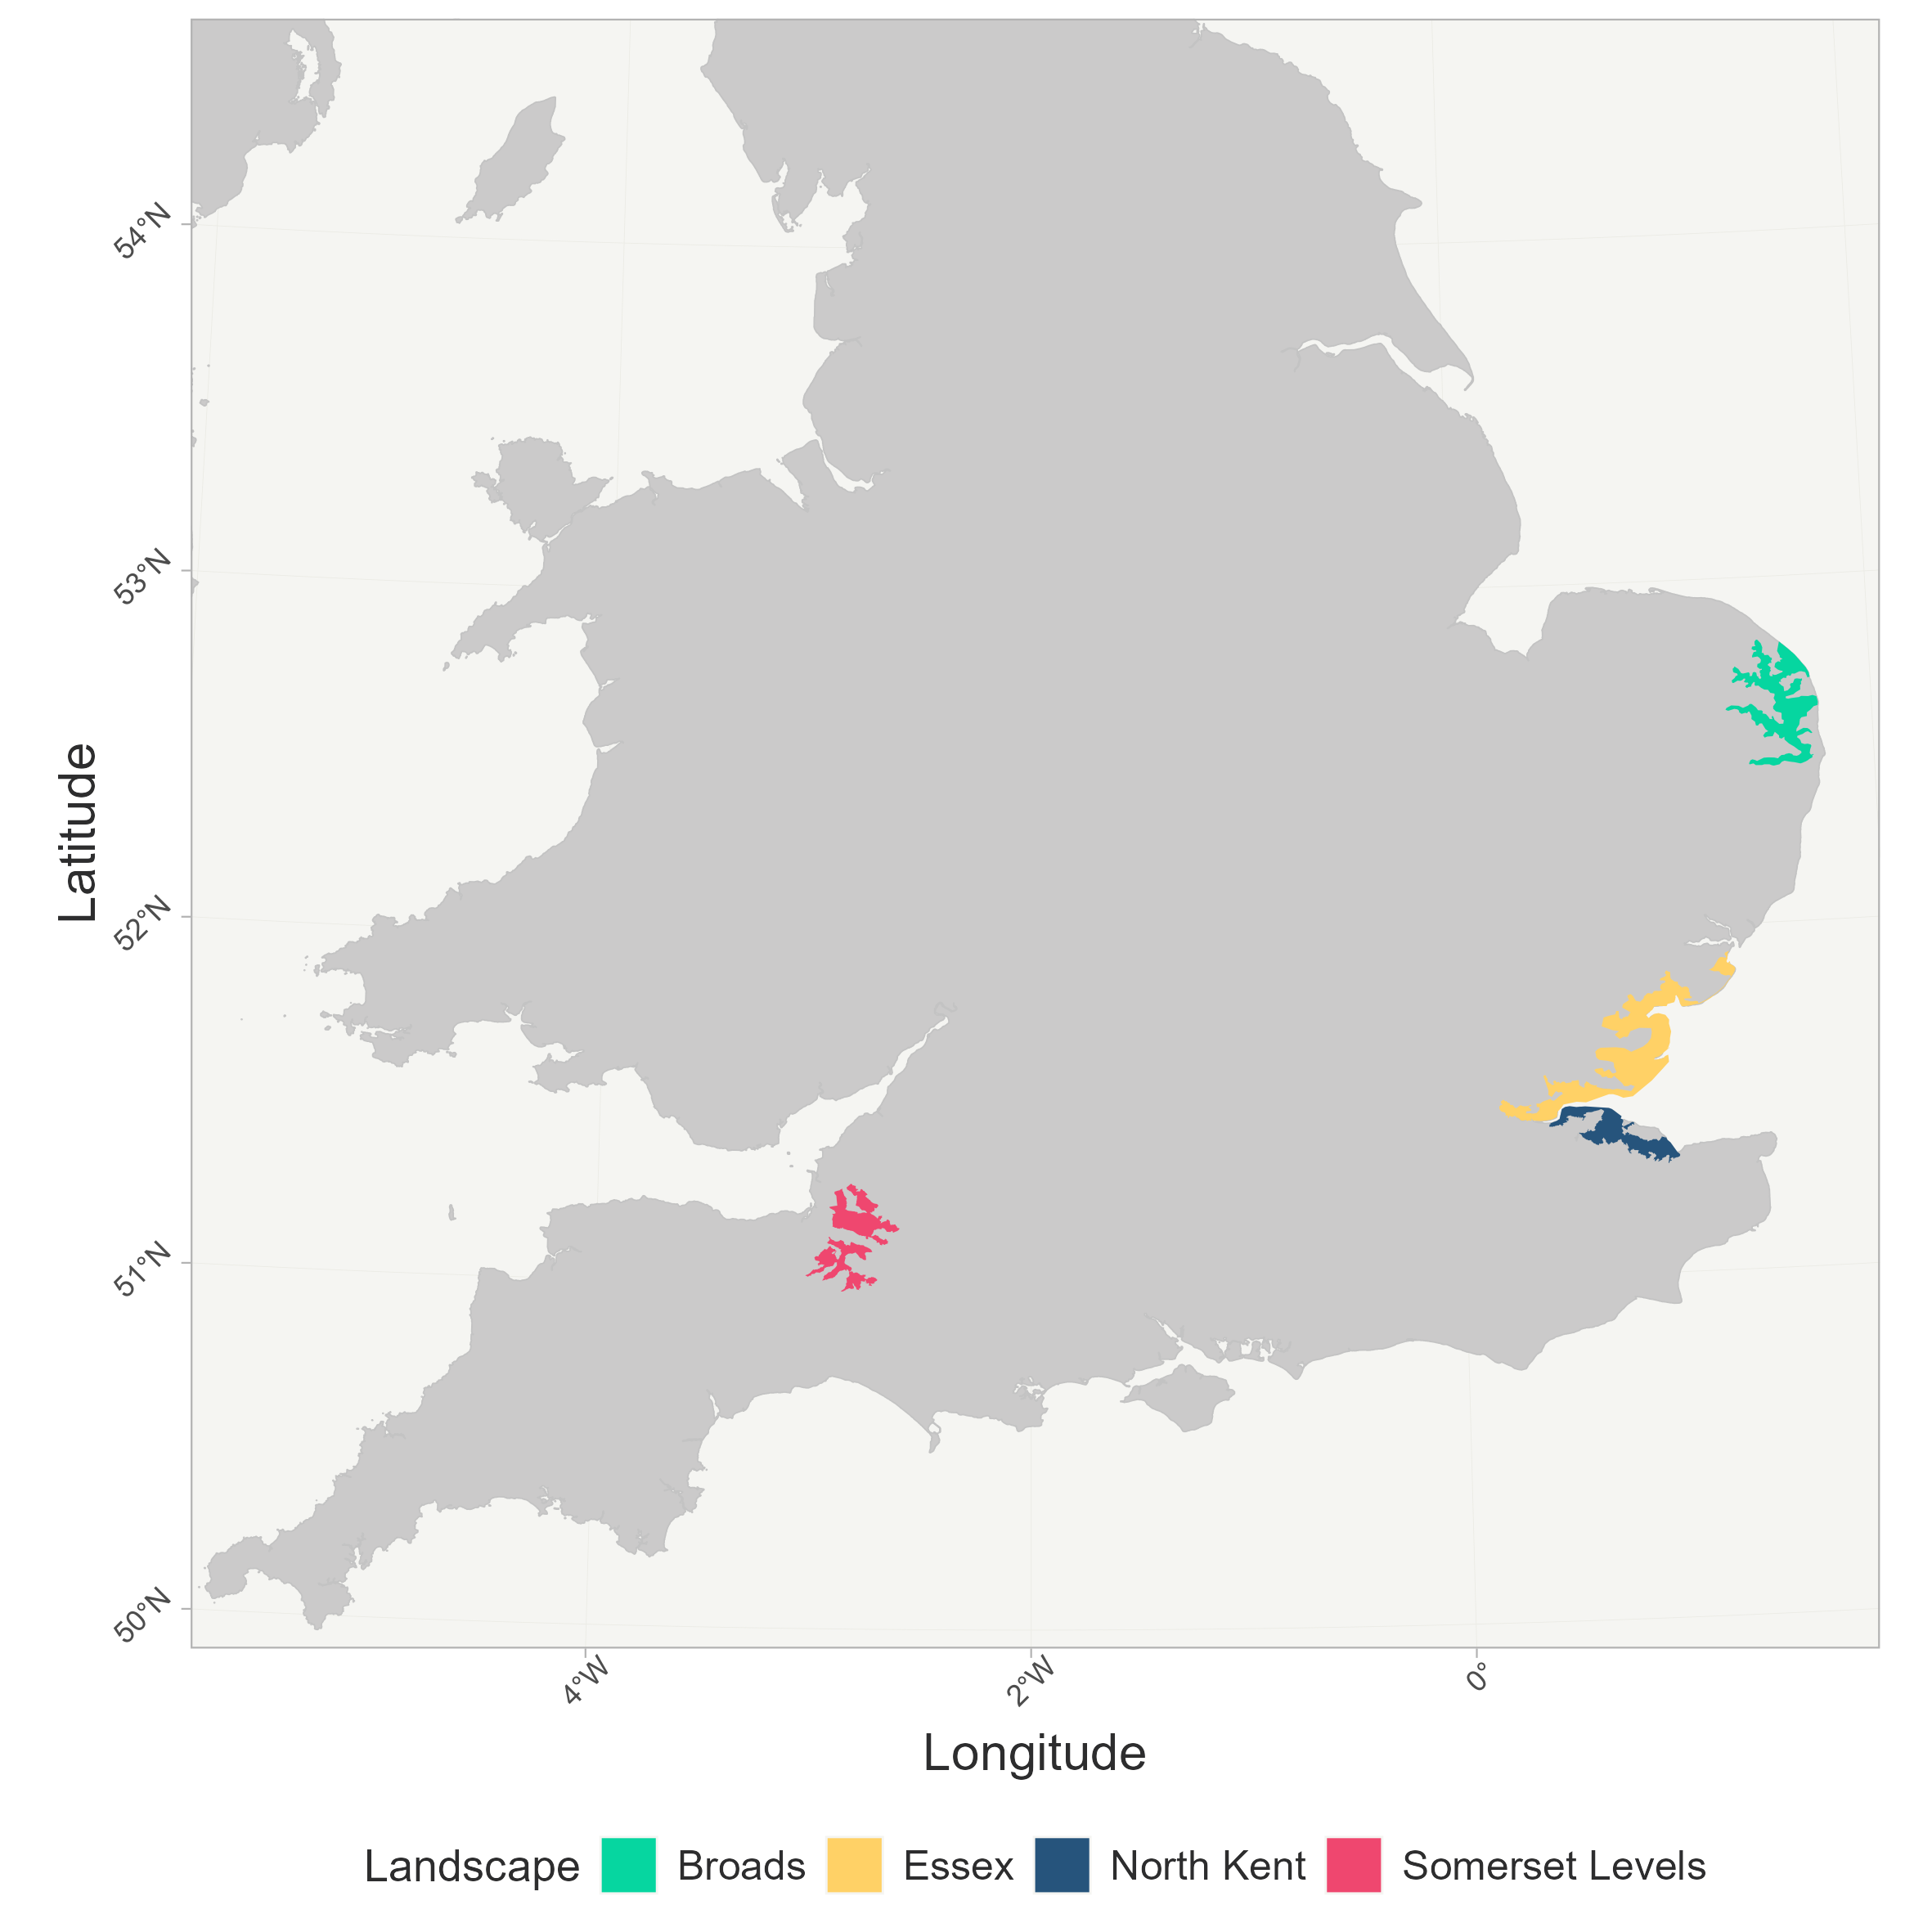
\includegraphics{qmdimages/AllLandscapePlots.png}

}

\caption{\label{fig-landscapes}Map of the four case-study landscapes
from this study. Essex and North Kent were formerly part of the same
``priority landscape'' but split due to differing characteristics and
geographic seperation.}

\end{figure}%

We ran stakeholder workshops across four different landscapes to
understand where it is possible to deploy these strategies according to
people who live and work in the area, thereby trying to link theory to
real world situations and landscapes. We focus on three different
`priority landscapes' (formerly known as Environmentally Sensitive
Areas, (\citeproc{ref-nateng2024}{Natural England 2024})): Somerset
Levels; Norfolk Broads (hereafter Broads); and Greater Thames (see
Figure~\ref{fig-landscapes}). We subsequently split the Greater Thames
landscape up into North Kent and Essex owing to differing land uses and
geographic separation. We chose these landscapes as they hold important
populations of breeding waders in a national context
(\citeproc{ref-wilson2005}{Wilson et al. 2005}) but also have different
characteristics (e.g.~soil types, land use compositions, wading bird
assemblages, uptake of AES and lowland wet grassland distribution, see
Table~\ref{tbl-scapestats} for landscape specific details). For North
Kent, Essex and the Broads we focus on Lapwing \emph{Vanellus vanellus}
and Redshank \emph{Tringa totanus} during the workshops and for the
Somerset Levels we focused on Lapwing and Snipe \emph{Gallinago
gallinago}. We focused on these species as they were the predominant
breeding wader species in each landscape. Curlews are a key part of the
breeding wader assemblage in the Somerset Levels but there were too few
survey records to build a model that predicted abundance, which was a
key aspect of the wider project.

Extensive breeding wader surveys were conducted in each landscape in
2021-22 as part of the national breeding wader of wet meadows survey. Up
to three visits during the breeding season were made to lowland wet
grassland fields (areas below 200m altitude subject to freshwater
flooding and water logging) with wading bird abundance and habitat
characteristics recorded. An optional fourth `dusk' visit was also
undertaken where Snipe breeding was suspected. As part of the wider
project, the four selected landscapes also received further visits in
2023 to survey areas that were missed in 2021-22.

\begin{table}

\caption{\label{tbl-scapestats}Charactericists for each of the four case
study landscapes. The breeding pairs for each landscapes were estimated
from the breeding waders of wet meadows survey. The total hectarage for
AES excludes reserves that also have AES agreements.}

\centering{

\centering\begingroup\fontsize{10}{12}\selectfont

\begin{tabular}[t]{>{\raggedright\arraybackslash}p{11.5em}>{\raggedright\arraybackslash}p{7.25em}>{\raggedright\arraybackslash}p{7.25em}>{\raggedright\arraybackslash}p{7.25em}>{\raggedright\arraybackslash}p{7.25em}}
\toprule
\begingroup\fontsize{12}{14}\selectfont \textbf{ }\endgroup & \begingroup\fontsize{12}{14}\selectfont \textbf{Broads}\endgroup & \begingroup\fontsize{12}{14}\selectfont \textbf{Essex}\endgroup & \begingroup\fontsize{12}{14}\selectfont \textbf{North Kent}\endgroup & \begingroup\fontsize{12}{14}\selectfont \textbf{Somerset}\endgroup\\
\midrule
\cellcolor{gray!10}{Total Area (ha)} & \cellcolor{gray!10}{43,138} & \cellcolor{gray!10}{72,342} & \cellcolor{gray!10}{22,798} & \cellcolor{gray!10}{30,905}\\
\addlinespace
Reserve LWG area (ha) & 1,151 & 1,636 & 2,151 & 1,204\\
\addlinespace
\cellcolor{gray!10}{AES only LWG area (ha)} & \cellcolor{gray!10}{5,068} & \cellcolor{gray!10}{1,279} & \cellcolor{gray!10}{1,976 ha} & \cellcolor{gray!10}{3,078}\\
\addlinespace
LWG type & Floodplain & Coastal & Coastal & Floodplain\\
\addlinespace
\cellcolor{gray!10}{Land use} & \cellcolor{gray!10}{Mixed arable \& grassland} & \cellcolor{gray!10}{Mainly arable, some grassland} & \cellcolor{gray!10}{Mainly grassland, some arable} & \cellcolor{gray!10}{Mainly grassland}\\
\addlinespace
Soil Type & Mixed mineral \& organic & Mainly mineral & Mainly mineral & Mainly organic, some mineral\\
\addlinespace
\cellcolor{gray!10}{Breeding Pairs} & \cellcolor{gray!10}{775} & \cellcolor{gray!10}{825} & \cellcolor{gray!10}{1575} & \cellcolor{gray!10}{225}\\
\addlinespace
Predominant Species & Lapwing/Redshank & Lapwing/Redshank & Lapwing/Redshank & Snipe\\
\bottomrule
\end{tabular}
\endgroup{}

}

\end{table}%

\subsection{Methods}\label{methods}

\subsubsection{Workshop Aim}\label{workshop-aim}

To create a map of future opportunity for wader conservation for each
stakeholder group within each landscape.

This can consist of preferences of where wader conservation could occur
as well as defining areas where wader conservation should be avoided.
These preferences can also be linked to specific nature restoration
strategies (better, bigger, more) and where arable land could be
reverted back to lowland wet grassland so that the map of future
opportunity can vary depending on the strategy.

\subsubsection{Workshop Attendees}\label{workshop-attendees}

We ran four regional workshops and we aimed to have three different
stakeholder groups attend each workshop. The three different groups (and
organisations invited) were:

\begin{itemize}
\tightlist
\item
  Conservationists (RSPB, Wildlife Trust, Wildfowl and wetland trust and
  Private nature reserves)
\item
  Public bodies (Natural England, Environment Agency, Internal drainage
  board, Local Authorities, Ministry of Defense, regional Farming and
  Wildlife Advisory Group rep)
\item
  Land managers (land owners, farmers, tenant farmers)
\end{itemize}

These groups were created to align participants in terms of background.
This helped to drive more productive group discussions and made it more
likely that a consensus would be reached during group activities. The
people invited to the workshops were largely already known to regional
RSPB members of staff. This may slightly bias the group of people that
attended towards those with more of an understanding and preference for
conservation. This could have particularly affected the land managers
group, for example some tenant farmers rent RSPB land for cattle grazing
or carry out wader friendly management on their own farm. This could
result in outputs are not fully representative of the wider stakeholder
group. Overall, we felt that this bias was tolerable and that a group of
more like minded participants would lead to more productive
conversations and ultimately result in more usable outputs.

In the end it was not possible to run all three group of stakeholders in
each priority landscape, apart from the Somerset Levels. We were only
able to run the activities with two groups in three of the landscape,
see Table~\ref{tbl-GrpAtt} for a breakdown of group attendance.

\begin{table}

\caption{\label{tbl-GrpAtt}Workshop attendance for the three different
stakeholder groups across the four priority landscapes. Note if only one
member of a stakeholder group attended a workshop then this individual
was gnerally moved into one of the other groups. Number of attendees for
each group is shown in brackets.}

\centering{

\centering\begingroup\fontsize{10}{12}\selectfont

\begin{tabular}[t]{llll}
\toprule
\begingroup\fontsize{12}{14}\selectfont \textbf{Landscape}\endgroup & \begingroup\fontsize{12}{14}\selectfont \textbf{Conservationists}\endgroup & \begingroup\fontsize{12}{14}\selectfont \textbf{Public Bodies}\endgroup & \begingroup\fontsize{12}{14}\selectfont \textbf{Land Managers}\endgroup\\
\midrule
\cellcolor{gray!10}{Broads} & \cellcolor{gray!10}{Y (5)} & \cellcolor{gray!10}{Y (7)} & \cellcolor{gray!10}{}\\
\addlinespace
Kent & Y (5) &  & Y (7)\\
\addlinespace
\cellcolor{gray!10}{Essex} & \cellcolor{gray!10}{Y (7)} & \cellcolor{gray!10}{} & \cellcolor{gray!10}{Y (7)}\\
\addlinespace
Somerset & Y (7) & Y (6) & Y (8)\\
\bottomrule
\end{tabular}
\endgroup{}

}

\end{table}%

\subsubsection{Workshop Activities}\label{workshop-activities}

In each workshop we gave an introductory presentation followed by three
stakeholder-led activities. The introductory presentation was in two
parts. Initially we presented the results from the 2021/22 breeding
waders of wet meadow survey, including the influence of habitat and land
management on breeding populations and the distribution of populations
within the landscape. Maps were also provided to participants to the
show the distribution of breeding wader populations and the layout of
different land uses within the priority landscape. Throughout all
activities, we told participants to focus on land within the priority
landscape; that the conservation of Lapwing and Redshank was a priority
(Lapwing and Snipe in the Somerset Levels); and to imagine what could be
possible in the year 2050.

After the presentation we ran three activities. We show below how each
task was presented to participants during the workshops.

\begin{itemize}
\tightlist
\item
  Activity 1

  \begin{itemize}
  \tightlist
  \item
    For each wader habitat intervention card discuss the challenges and
    opportunities. These can be associated with certain areas,
    land-uses, farming practices, costs/funding or practicalities.
    Mediators will record your discussion on the back of each card.
  \item
    After the cards provided record any other interventions on the blank
    cards provided and discuss their challenges/opportunities.
  \item
    The cards depicted the following interventions or management
    strategies for breeding waders: keeping standing water throughout
    spring; foot drain/scrape creation for wet surface features; grazing
    to create a varied sward; rush control; delayed cutting on
    hay/silage fields; predator exclusion using fences; and predator
    control.
  \end{itemize}
\item
  Activity 2

  \begin{itemize}
  \tightlist
  \item
    Discuss any goals for breeding waders. For example, how many waders,
    in the landscape and which species?
  \item
    Are their existing landscape plans that could influence breeding
    waders?
  \item
    Choose conservation strategies and rank them (better, bigger, more
    and arable reversion). If you can't rank strategies choose priority
    ones.
  \end{itemize}
\item
  Activity 3

  \begin{itemize}
  \tightlist
  \item
    Create guidelines for where each strategy can (preference) and can't
    (avoidance) be used.
  \item
    Mention any data sources that could be used to create the
    guidelines. Are there specific cut-off points associated with any of
    the guidelines?
  \end{itemize}
\end{itemize}

Activity 1 was designed as a primer activity and while we recorded the
main points of discussions within stakeholder groups there were no main
outputs from this activity. This activity was designed to initiate
conversations about wader conservation and the challenges and
opportunities in its implementation. This activity helped spark ideas
for further activities as it identified where management for breeding
waders would be the easiest or hardest to implement (see activity 3).

Activity 2 was designed as another primer activity but we planned that
some of these tasks would feed into other aspects of this project
(i.e.~scenario modelling). Participants discussed goals for breeding
waders and identified existing plans that and these discussion fed into
the scenario modelling part of the project. Participants also discussed
and ranked conservation strategies which was used as a primer for the
final task so stakeholders could discuss where their priorities lay
between the following conservation strategies: 1) improving existing
breeding wader sites (better); 2) expanding existing wader sites
(bigger); 3) creating new sites for breeding wader (more); and 4)
converting arable land to lowland wet grassland for breeding waders.
Although arable reversion is not a Lawton principle, it was defined as a
separate option here because stakeholder preferences for wet grassland
creation could markedly differ between existing unsuitable grassland and
arable land, i.e.~preferring reversion of arable land on peaty soils or
specific crop types.

Activity 3 generated the main outputs presented in this report and
stakeholder generally spent more time on this task than on the other two
activities combined. The purpose of this task was for stakeholders to
create preferences or avoidance guidelines for where breeding wader
conservation could or could not occur within the landscape. Preferences
were guidelines that could essentially grade the land into areas of
differing favorability, e.g.~prefer breeding wader conservation on lower
lying land. Avoidance rules mapped out where wader conservation would
not be carried out, e.g.~avoiding areas of priority habitat lowland fen.
Preferences could also be linked to one, multiple or all the
conservation strategies outlined in activity 2 (i.e.~better, bigger,
more, arable reversion). For example, preferring conservation efforts in
the smallest existing breeding populations first was linked to the
improving existing wader strategy (better), whereas preferring
conservation efforts on lower lying land was often associated with all
of the conservation strategies. All avoidance guidelines created applied
to all the conservation strategies. During stakeholder discussions there
was filtering of guidelines by the facilitator to remove any guidelines
that we would not be able to map out spatially. If there was any doubt,
then the guideline was recorded and if it could not be used then a full
explanation is provided in the appendix.

\subsubsection{Compiling Preferences}\label{compiling-preferences}

For each landscape and stakeholder group combination we produced heat
maps for the main conservation strategies, better, bigger and more. We
also produced heat maps for the bigger and more strategies being
realized through arable reversion which involved combing the guidelines
for arable reversion and bigger or more. In total, for any stakeholder
group this meant the creation of 5 different heat maps.

Each guideline was mapped out onto a 25m x 25m base raster. Each
preference guideline became a continuous raster with pixels given a
value between 0 (least preferred) and 1 (most preferred) and avoidance
rules became a binary raster of 0 (no avoidance) and 1 (avoid). Next,
for each 25m x 25m cell, preference rules were subsequently aggregated
(summed) to produce an overall preference score. Note, for simplicity,
individual preference rules were treated as equal with no form of
weighting applied. Last, any cells that was classified as 1 for any of
the avoidance rules were excluded from the opportunity area,
irrespective of their preference score. A 25m x 25m pixel size was
chosen as this is the resolution of the UKCEH land cover maps
(\citeproc{ref-marston2022}{Marston et al. 2022}) that was used to
identify areas of suitable grassland and arable land for lowland we
grassland creation (see following section). For the creation of each
graded raster including the manipulation, processing and analysis we
used the packages \emph{sf} (\citeproc{ref-pebesma2018}{Pebesma 2018})
and \emph{terra} (\citeproc{ref-hijmans2024}{Hijmans 2024}) in the
programming language R (\citeproc{ref-R2023}{R Core Team 2023}).

\subsubsection{Defining Conservation Strategy
Extent}\label{defining-conservation-strategy-extent}

For each conservation strategy there were only certain areas within the
landscapes where the strategy could be realized. For all strategies,
creation of lowland wet grassland for breeding waders had to be carried
out on land where this habitat could feasibly be created. Areas were
often unsuitable due to topography, land use of soil type. For better,
bigger and more strategies this land had to currently be some form of
grassland. When any of these strategies were realized using arable
reversion then the starting land use had to be arable. In addition, for
the strategy to improve existing wader sites (better) we had to define
where existing wader sites were within the landscape. Any areas outside
of defined wader sites could be used to expand existing sites (bigger)
or create more sites (more). We go into detail of how we define land
that has the right characteristics to be lowland wet grassland; current
arable land; and breeding wader sites below.

\paragraph{Defining candidate lowland wet grassland for
restoration}\label{defining-candidate-lowland-wet-grassland-for-restoration}

We defined current grassland that has the right characteristics,
i.e.~elevation and soil type, to be areas where high quality lowland wet
grassland could be created, regardless of its current condition.
Therefore, this included current high-quality lowland wet grassland as
well as dry grassland with drainage. This mapping exercise was done
using a base raster with a resolution of 25 meters. Potential lowland
wet grassland pixels included fields considered for survey from the
2021/2022 BWWM survey Hawkes et al in press. These fields were
historically defined as periodically water-logged permanent grassland
below 200 meters above sea level, including grazing marshes, flood
meadows, man-made washlands, and water meadows. We supplemented this
with areas of semi-natural grassland habitats (Coastal and floodplain
grazing marsh; Good quality semi-improved grassland; Lowland meadows;
and Purple moor grass and rush pastures) from the Natural England's
priority habitat index (\citeproc{ref-natengland2022}{Natural England
2022}). These supplementary areas also had to overlap with peaty or
seasonally wet soils from the NATMAP soil vector data (see
Table~\ref{tbl-wetsoil} for a full list of acceptable soil types
(\citeproc{ref-nsri2022}{NSRI 2022})) and be at an elevation below the
99.5th quantile of all elevation values within field included in the
2021/2022 BWWM survey (Hawkes et al in press). These criteria prevented
fields at high elevations being included. Since both data sets were
created more before the year of the study we masked out any pixels
classified as non-grassland habitats from any of the UKCEH landcover
datasets from 2021 (\citeproc{ref-marston2022}{Marston et al. 2022}),
2022 (\citeproc{ref-marston2024}{Marston et al. 2024}), or 2023
(\citeproc{ref-morton2024}{Morton et al. 2024}). Finally, we visually
checked every map to remove obvious arable land, woodland, salt marsh,
and golf courses.

In the Somerset Levels and Norfolk Broads in particular, small pockets
of trees were not detected in the UKCEH land cover data sets. To remove
all trees, we created a canopy model by subtracting the digital terrain
model (\citeproc{ref-envagency2023a}{Environment Agency 2023a}) from the
first pass digital surface model
(\citeproc{ref-envagency2023b}{Environment Agency 2023b}) from the
Environment Agency National Lidar Programme dataset. This canopy model
had a resolution of 1 meter, which we transformed to our base resolution
using nearest neighbor interpolation. We then used this layer to mask
out any pixels with a canopy height greater than 2 meters.

\begin{table}

\caption{\label{tbl-wetsoil}List of soil types from the NATMAP vector of
soil types that were to be seasonally wet or peaty soils}

\centering{

\centering\begingroup\fontsize{10}{12}\selectfont

\begin{tabular}[t]{l}
\toprule
\begingroup\fontsize{12}{14}\selectfont \textbf{Soil types}\endgroup\\
\midrule
\cellcolor{gray!10}{Fen peat soils}\\
\addlinespace
Lime-rich loamy and clayey soils with impeded drainage\\
\addlinespace
\cellcolor{gray!10}{Loamy and clayey floodplain soils with naturally high groundwater}\\
\addlinespace
Loamy and clayey soils of coastal flats with naturally high groundwater\\
\addlinespace
\cellcolor{gray!10}{Loamy and sandy soils with naturally high groundwater and a peaty surface}\\
\addlinespace
Loamy soils with naturally high groundwater\\
\addlinespace
\cellcolor{gray!10}{Naturally wet very acid sandy and loamy soils}\\
\addlinespace
Raised bog peat soils\\
\addlinespace
\cellcolor{gray!10}{Slightly acid loamy and clayey soils with impeded drainage}\\
\addlinespace
Slowly permeable seasonally wet acid loamy and clayey soils\\
\addlinespace
\cellcolor{gray!10}{Slowly permeable seasonally wet slightly acid but base-rich loamy and clayey soils}\\
\bottomrule
\end{tabular}
\endgroup{}

}

\end{table}%

\paragraph{Defining candidate arable land for
restoration}\label{defining-candidate-arable-land-for-restoration}

To identify arable land that could be reverted to high quality lowland
wet grassland we used a similar method to above. We first identified any
land that overlapped with peaty or seasonally wet soils from the NATMAP
soil vector data (\citeproc{ref-nsri2022}{NSRI 2022}). This land also
had to be at an elevation below the 99.5th quantile of all elevation
values within field included in the 2021/2022 BWWM survey (Hawkes et al
in press). We then identified arable pixels as any that were identified
as arable in at least two of the UKCEH landcover datasets from 2021
(\citeproc{ref-marston2022}{Marston et al. 2022}), 2022
(\citeproc{ref-marston2024}{Marston et al. 2024}), or 2023
(\citeproc{ref-morton2024}{Morton et al. 2024}). Finally, we visually
checked every map to remove obvious woodland, salt marsh, and golf
courses and for the Somerset Levels and Norfolk Broads we used the same
tree mask as described above.

\paragraph{Defining existing wader
sites}\label{defining-existing-wader-sites}

There is no set definition of what an existing site for nature is, and
it could be quantified using habitat type, habitat quality or the
current distribution of species. We took the approach that existing
sites for breeding wader were the areas already occupied by breeding
waders. We used field-level data from the breeding waders of wet meadows
survey in 2021/22 and further gap filling surveys in 2023 to define
breeding wader sites. A field was defined as occupied if the number of
estimated breeding pairs of Lapwing, Redshank or Snipe in a field was
greater than 1 (see (\citeproc{ref-smart2014}{Smart et al. 2014}) for
pair estimation methods). We then created polygons around clusters of
occupied fields and defined these as breeding wader sites. This
clustering approach was used, instead of just using the occupied field
centroids, as it allowed us to capture suitable fields recorded as
unoccupied due to imperfect detection or factors other than habitat
quality. For example, some large reserves have large areas of suitable
habitat but not every single parcel is occupied by breeding waders. As
we did not carry out breeding surveys over the entire landscapes, this
approach could have missed some small breeding populations. However, for
all four landscapes, all sites with known wader populations were
surveyed unless access was denied. We consulted with regional
conservationist and recording bodies to confirm that the surveys did not
miss any previously known breeding populations. The full details of are
clustering approach are detailed below.

We used the centroids of all occupied fields to run a K-means clustering
analysis to identify distinct clusters of breeding wader fields within
each of the four landscapes (Figure~\ref{fig-kmeansclust}). This
essentially creates k number of clusters while minimizing the within
cluster sum of squares. We explored a range of different values for k
between 2 and 25 and chose the one at the elbow of the relationship
between within cluster sum of squares and k. For all regions we selected
a value of 6 or 7 for k. This analysis was done using the \emph{kmeans}
function in the R package stats (\citeproc{ref-R2023}{R Core Team
2023}). For each of the identified clusters we then create a kernel
density estimate using the field centroids in each cluster. We created
95\% kernel density estimate boundaries using the \emph{hr\_kde} in the
R package amt (\citeproc{ref-signer2019}{Signer, Fieberg, and Avgar
2019}) and set the bandwidth parameter to the median field width for
each landscape. The median field width ranged from 155.7m in the
Somerset Levels to 233.4m in Essex. Any overlapping boundaries between
clusters were combined at this stage. This step allowed smoothed
polygons to be created around clusters and was preferable to using
minimum convex polygons as often single occupied fields, far from
cluster centers, expended cluster polygons into unsuitable habitat. With
these smoothed polygons we classified individual land parcels as within
`wader sites' if they were more than 50\% covered and that the habitat
was been previously identified as suitable for lowland wet grassland.
Finally, we removed any small sites that contained very few land parcels
or had a very small population of waders that were too small to be a
viable population. Therefore, we removed clusters that contained three
or less land parcels or three or less pairs of breeding waders
(Figure~\ref{fig-finalclusters}).

\begin{figure}[H]

\centering{

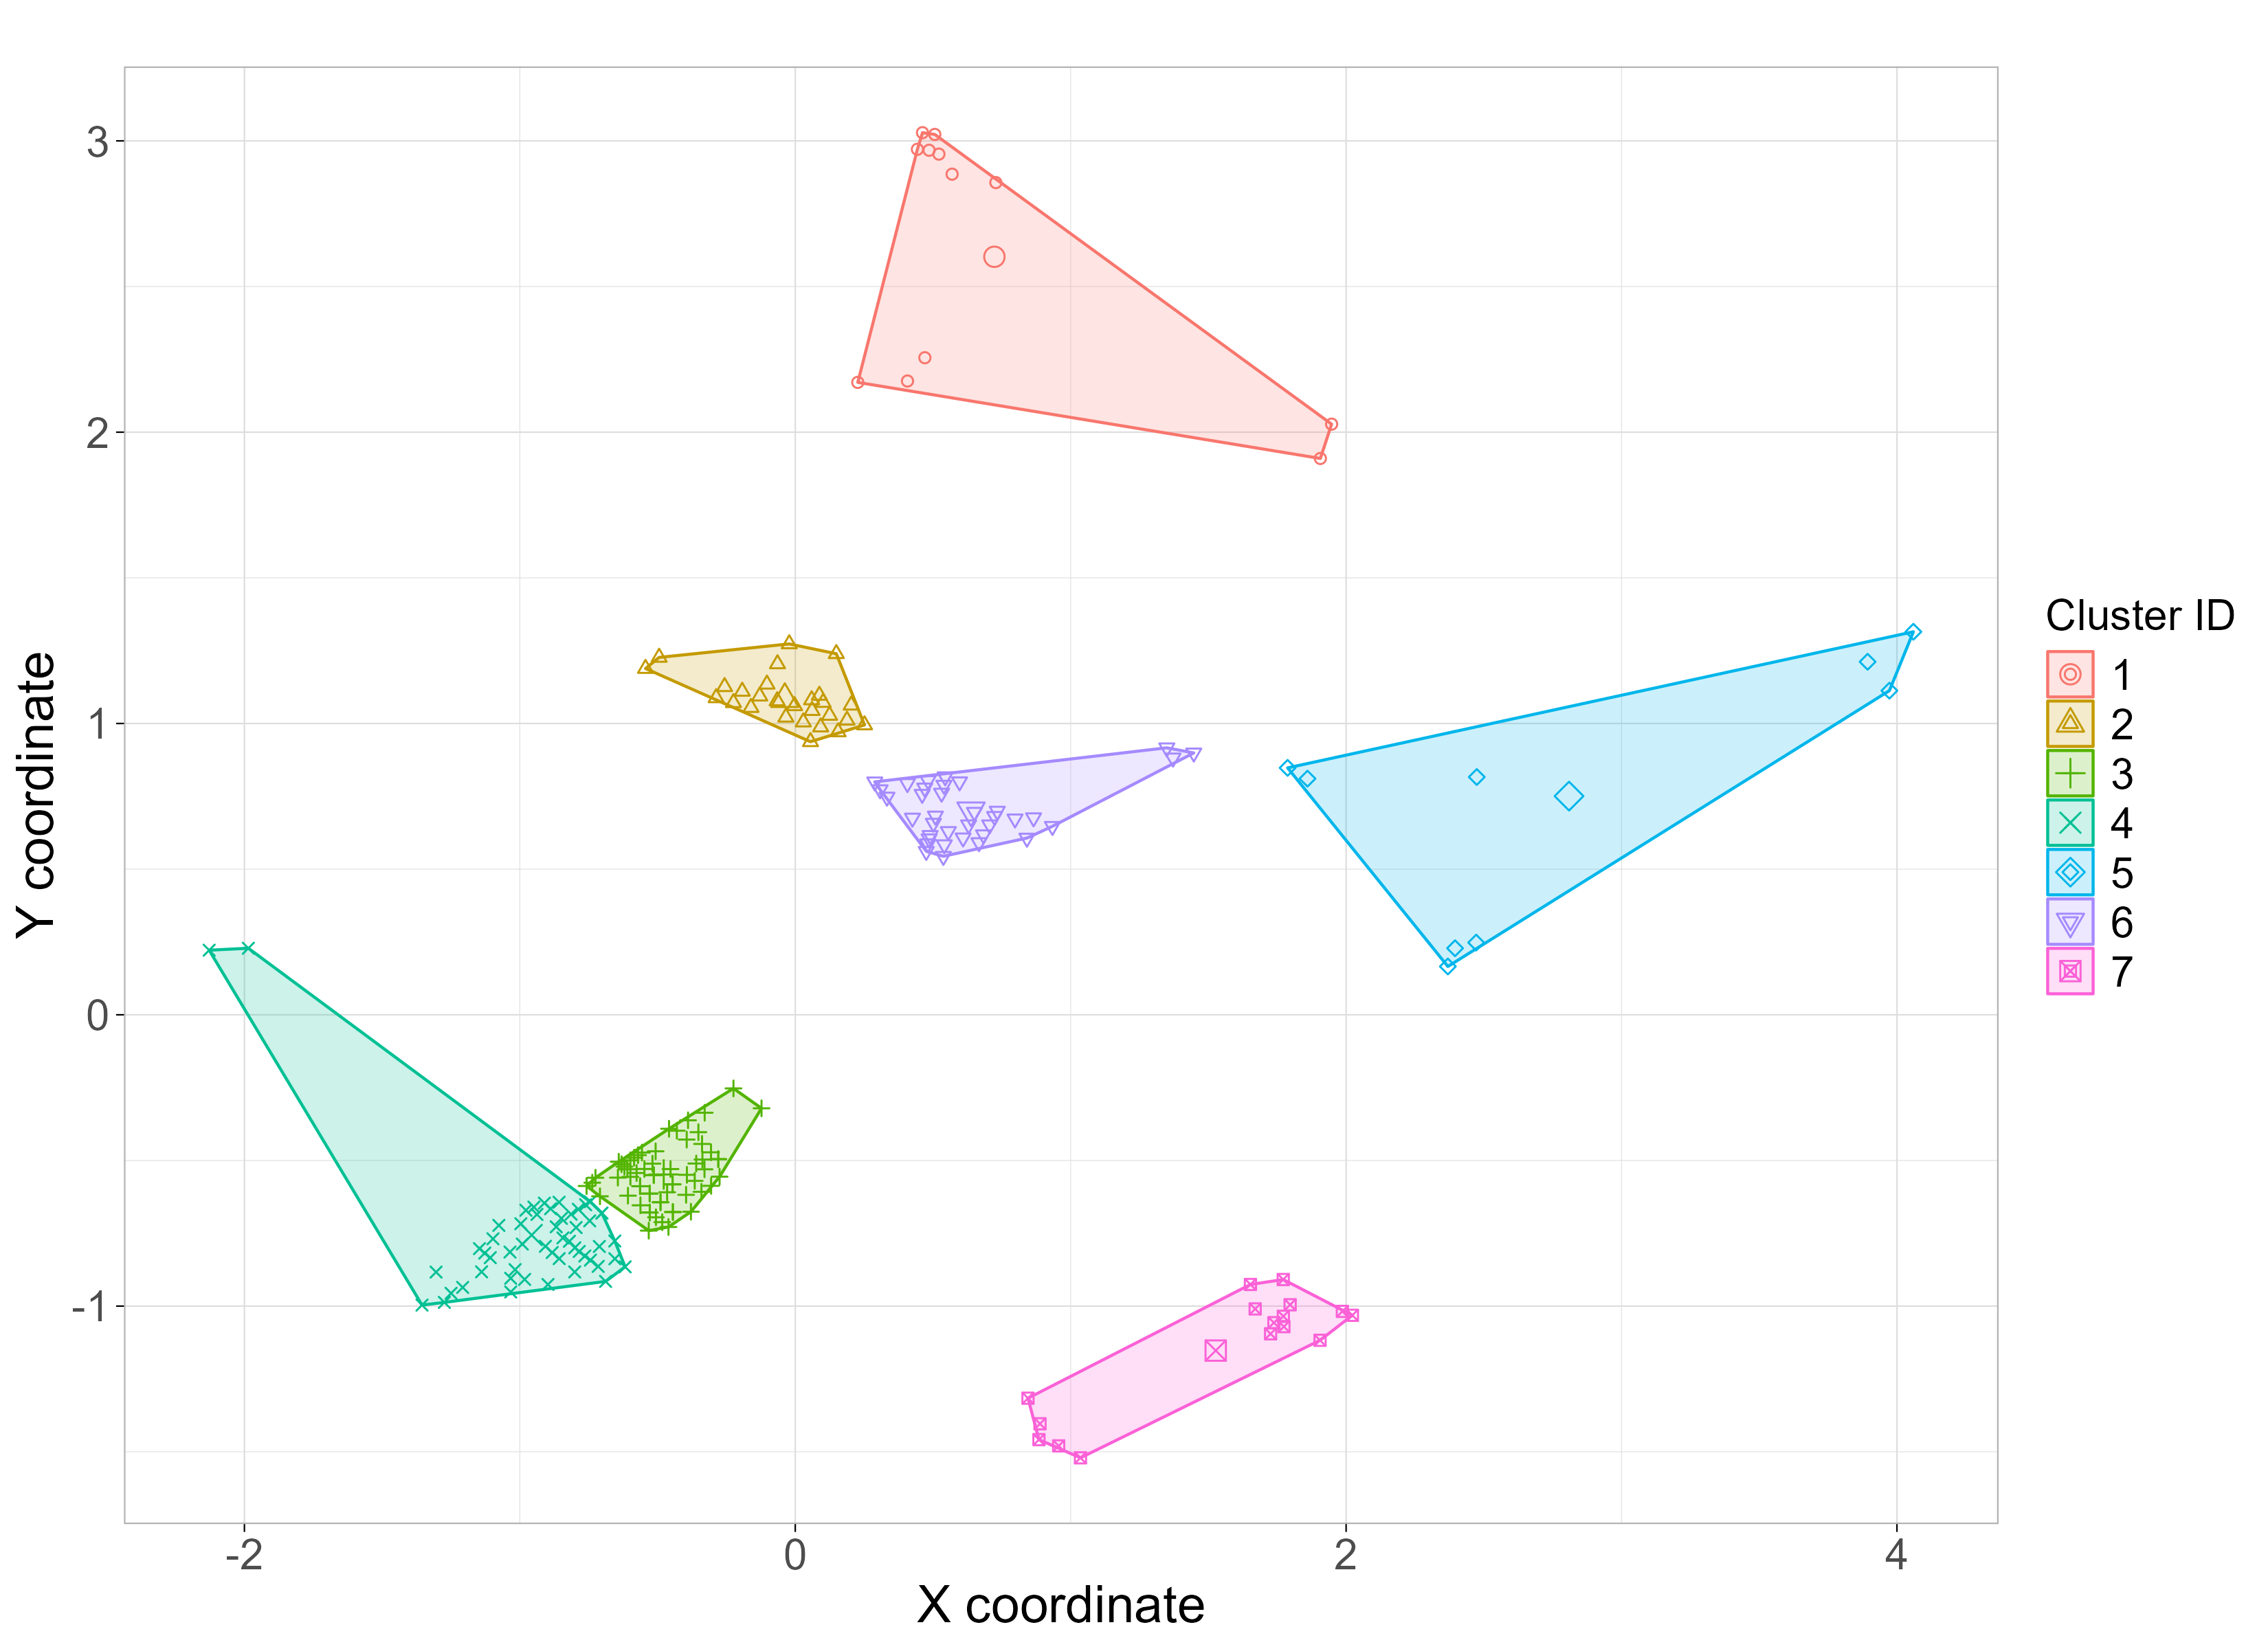
\includegraphics{qmdimages/Som_KmeansClusts.png}

}

\caption{\label{fig-kmeansclust}Results of k-mean clustering of field
centroids for land parcels occupied by breeding wader in the Somerset
Levels. A value of 7 for k was chosen based off the elbow point of the
relationship between within cluster sum of squares and k}

\end{figure}%

\begin{figure}[H]

\centering{

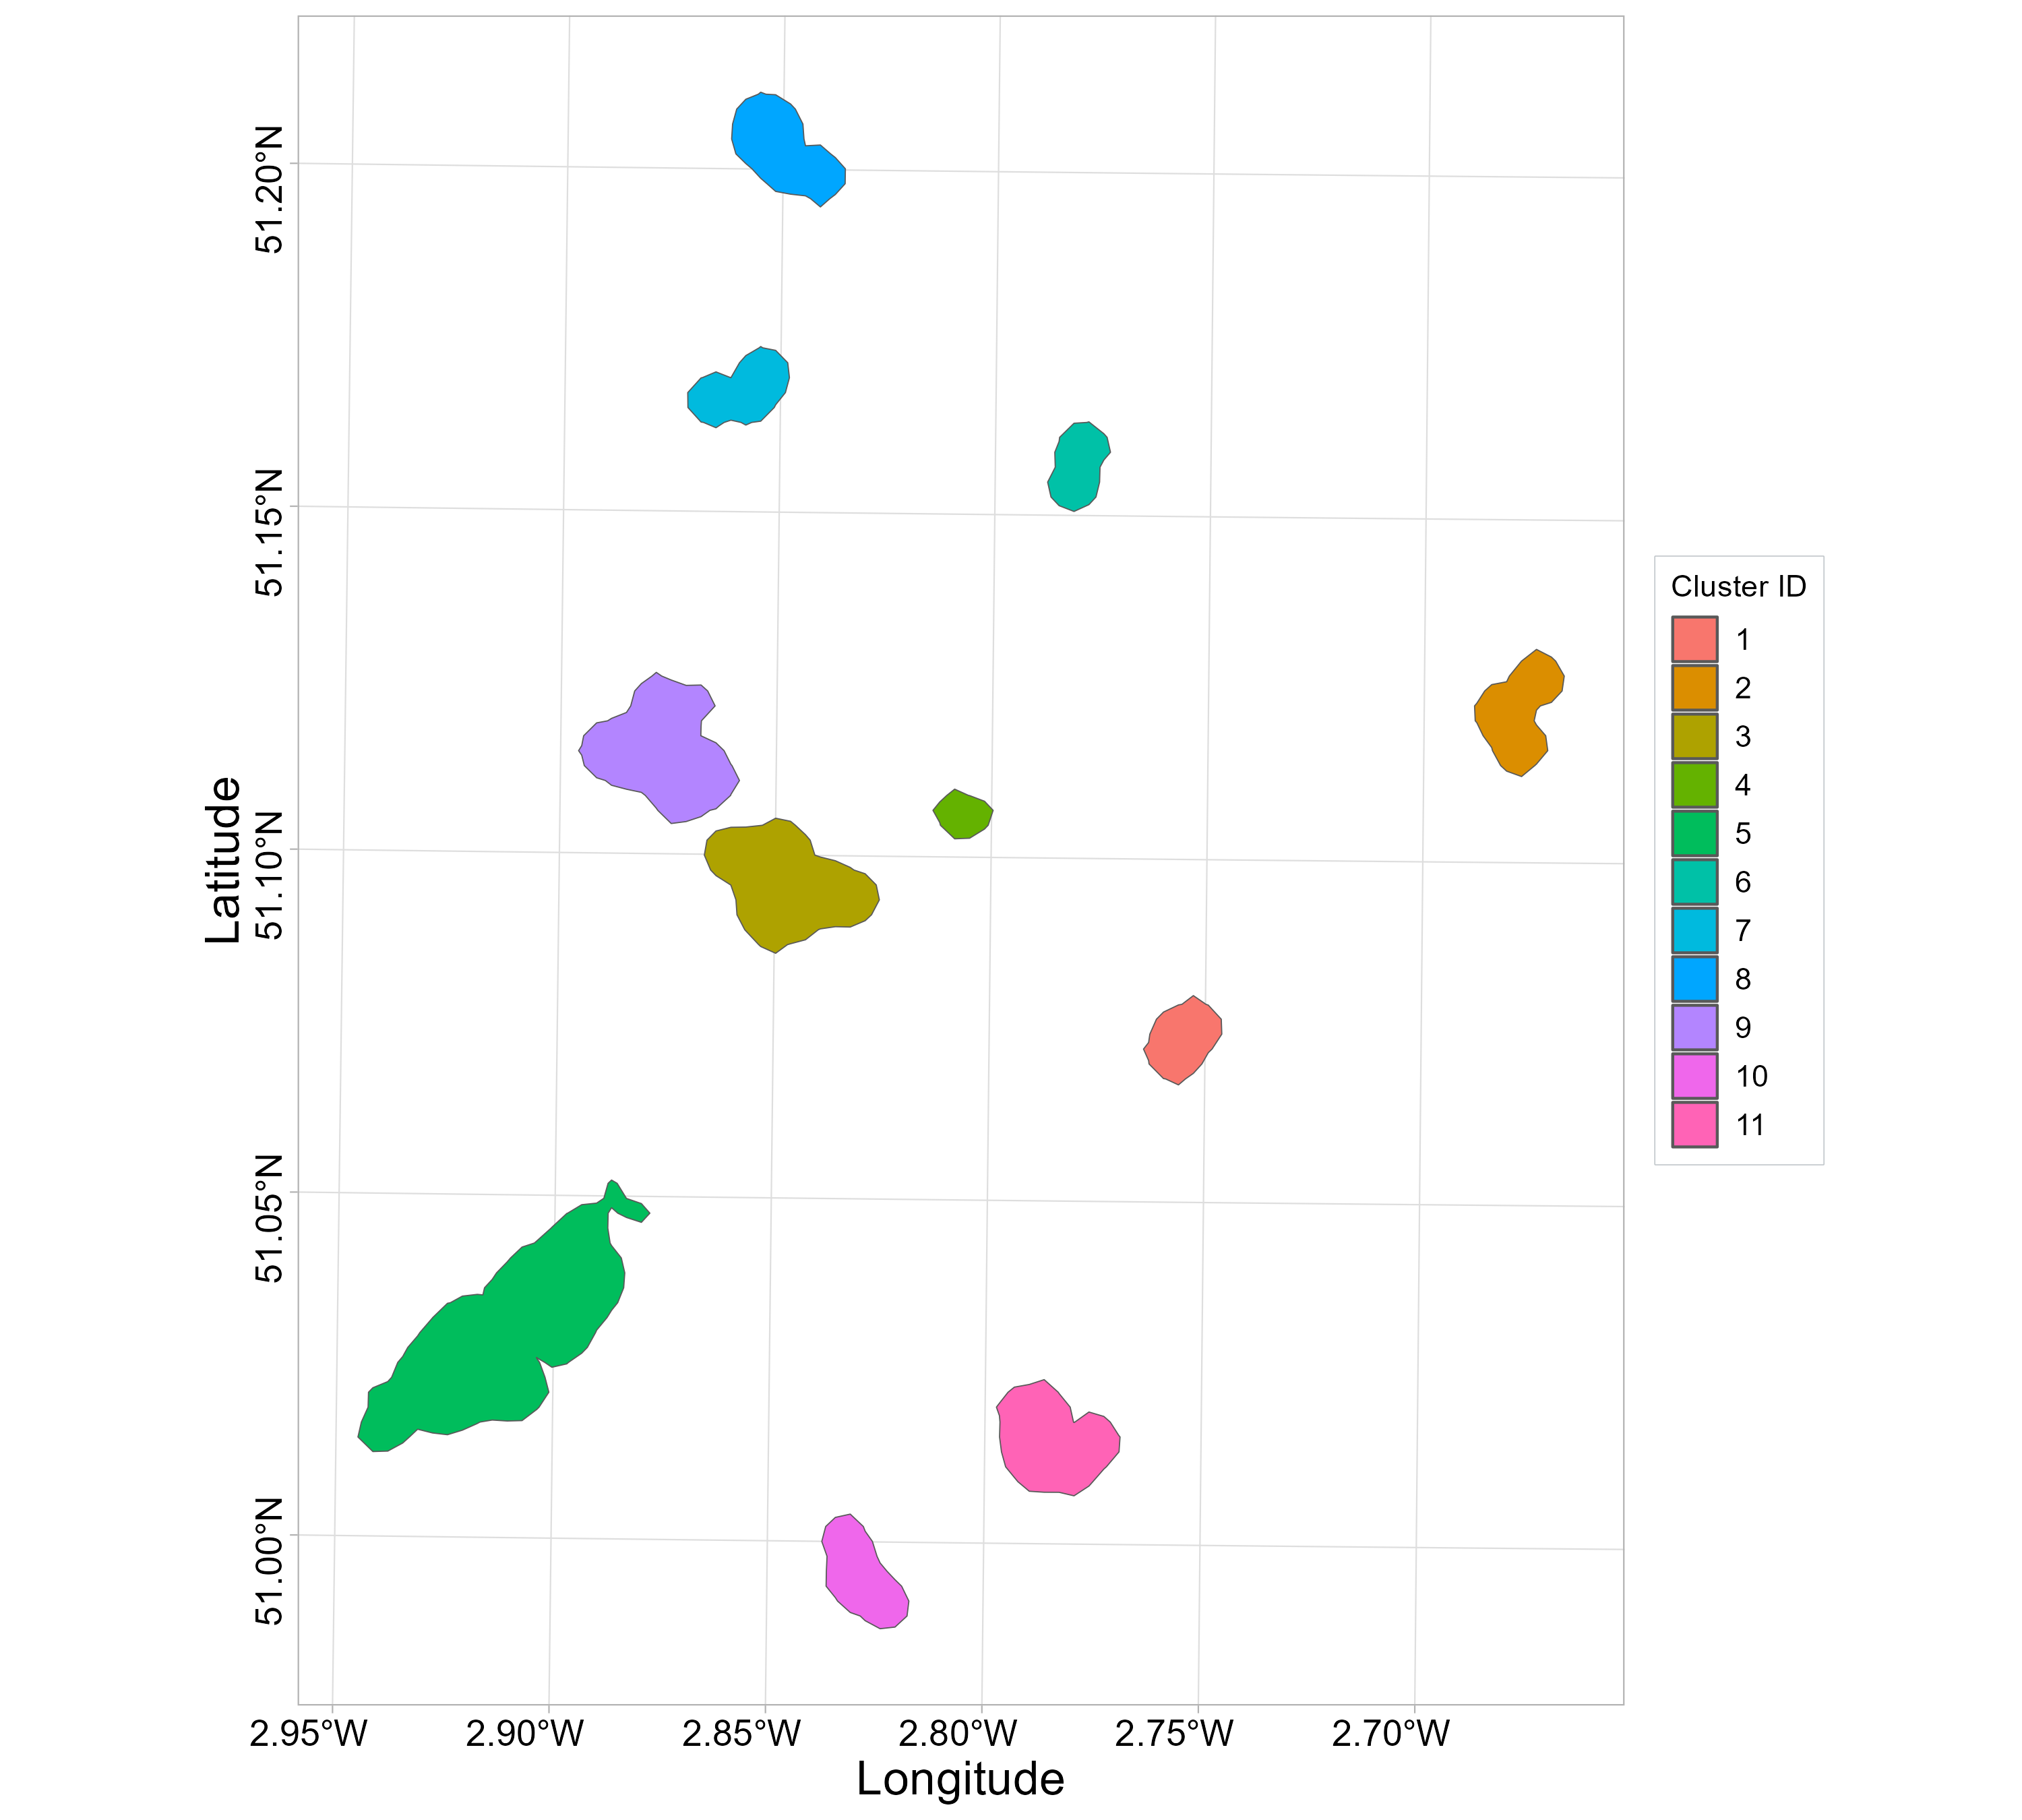
\includegraphics{qmdimages/Som_Final_clusters.png}

}

\caption{\label{fig-finalclusters}Final retained 95\% kernel density
estimate polygons of breeding wader clusters for the Somerset Levels.
Each cluster was treated as a separate site}

\end{figure}%

\subsubsection{Linking this work to the wider
project}\label{linking-this-work-to-the-wider-project}

INSERT TEXT HERE

\newpage{}

\subsection{Results \& Discussion}\label{results-discussion}

\subsubsection{Norfolk Broads Results}\label{norfolk-broads-results}

For the Norfolk Broads we had two different stakeholder groups. Group 1
(G1) was a group of conservationists and group 2 was a group of various
public body representatives tasked with wider objectives than the
preservation of biodiversity (e.g.~Natural England, Internal drainage
board, Broads Authority and Norfolk FWAG). The stakeholder guidelines
that were generated during the workshops and how these were converted
into a graded map can be found in Table~\ref{tbl-NorG1} for group 1 and
Table~\ref{tbl-NorG2} for group 2. The fields identified as grassland or
arable land that has the right characteristics to be lowland wet
grassland, regardless of it's current condition can be seen in
Figure~\ref{fig-BroadsSuitHab} and existing wader sits can be seen in
Figure~\ref{fig-BroadsLawton}.

\begin{figure}[H]

\centering{

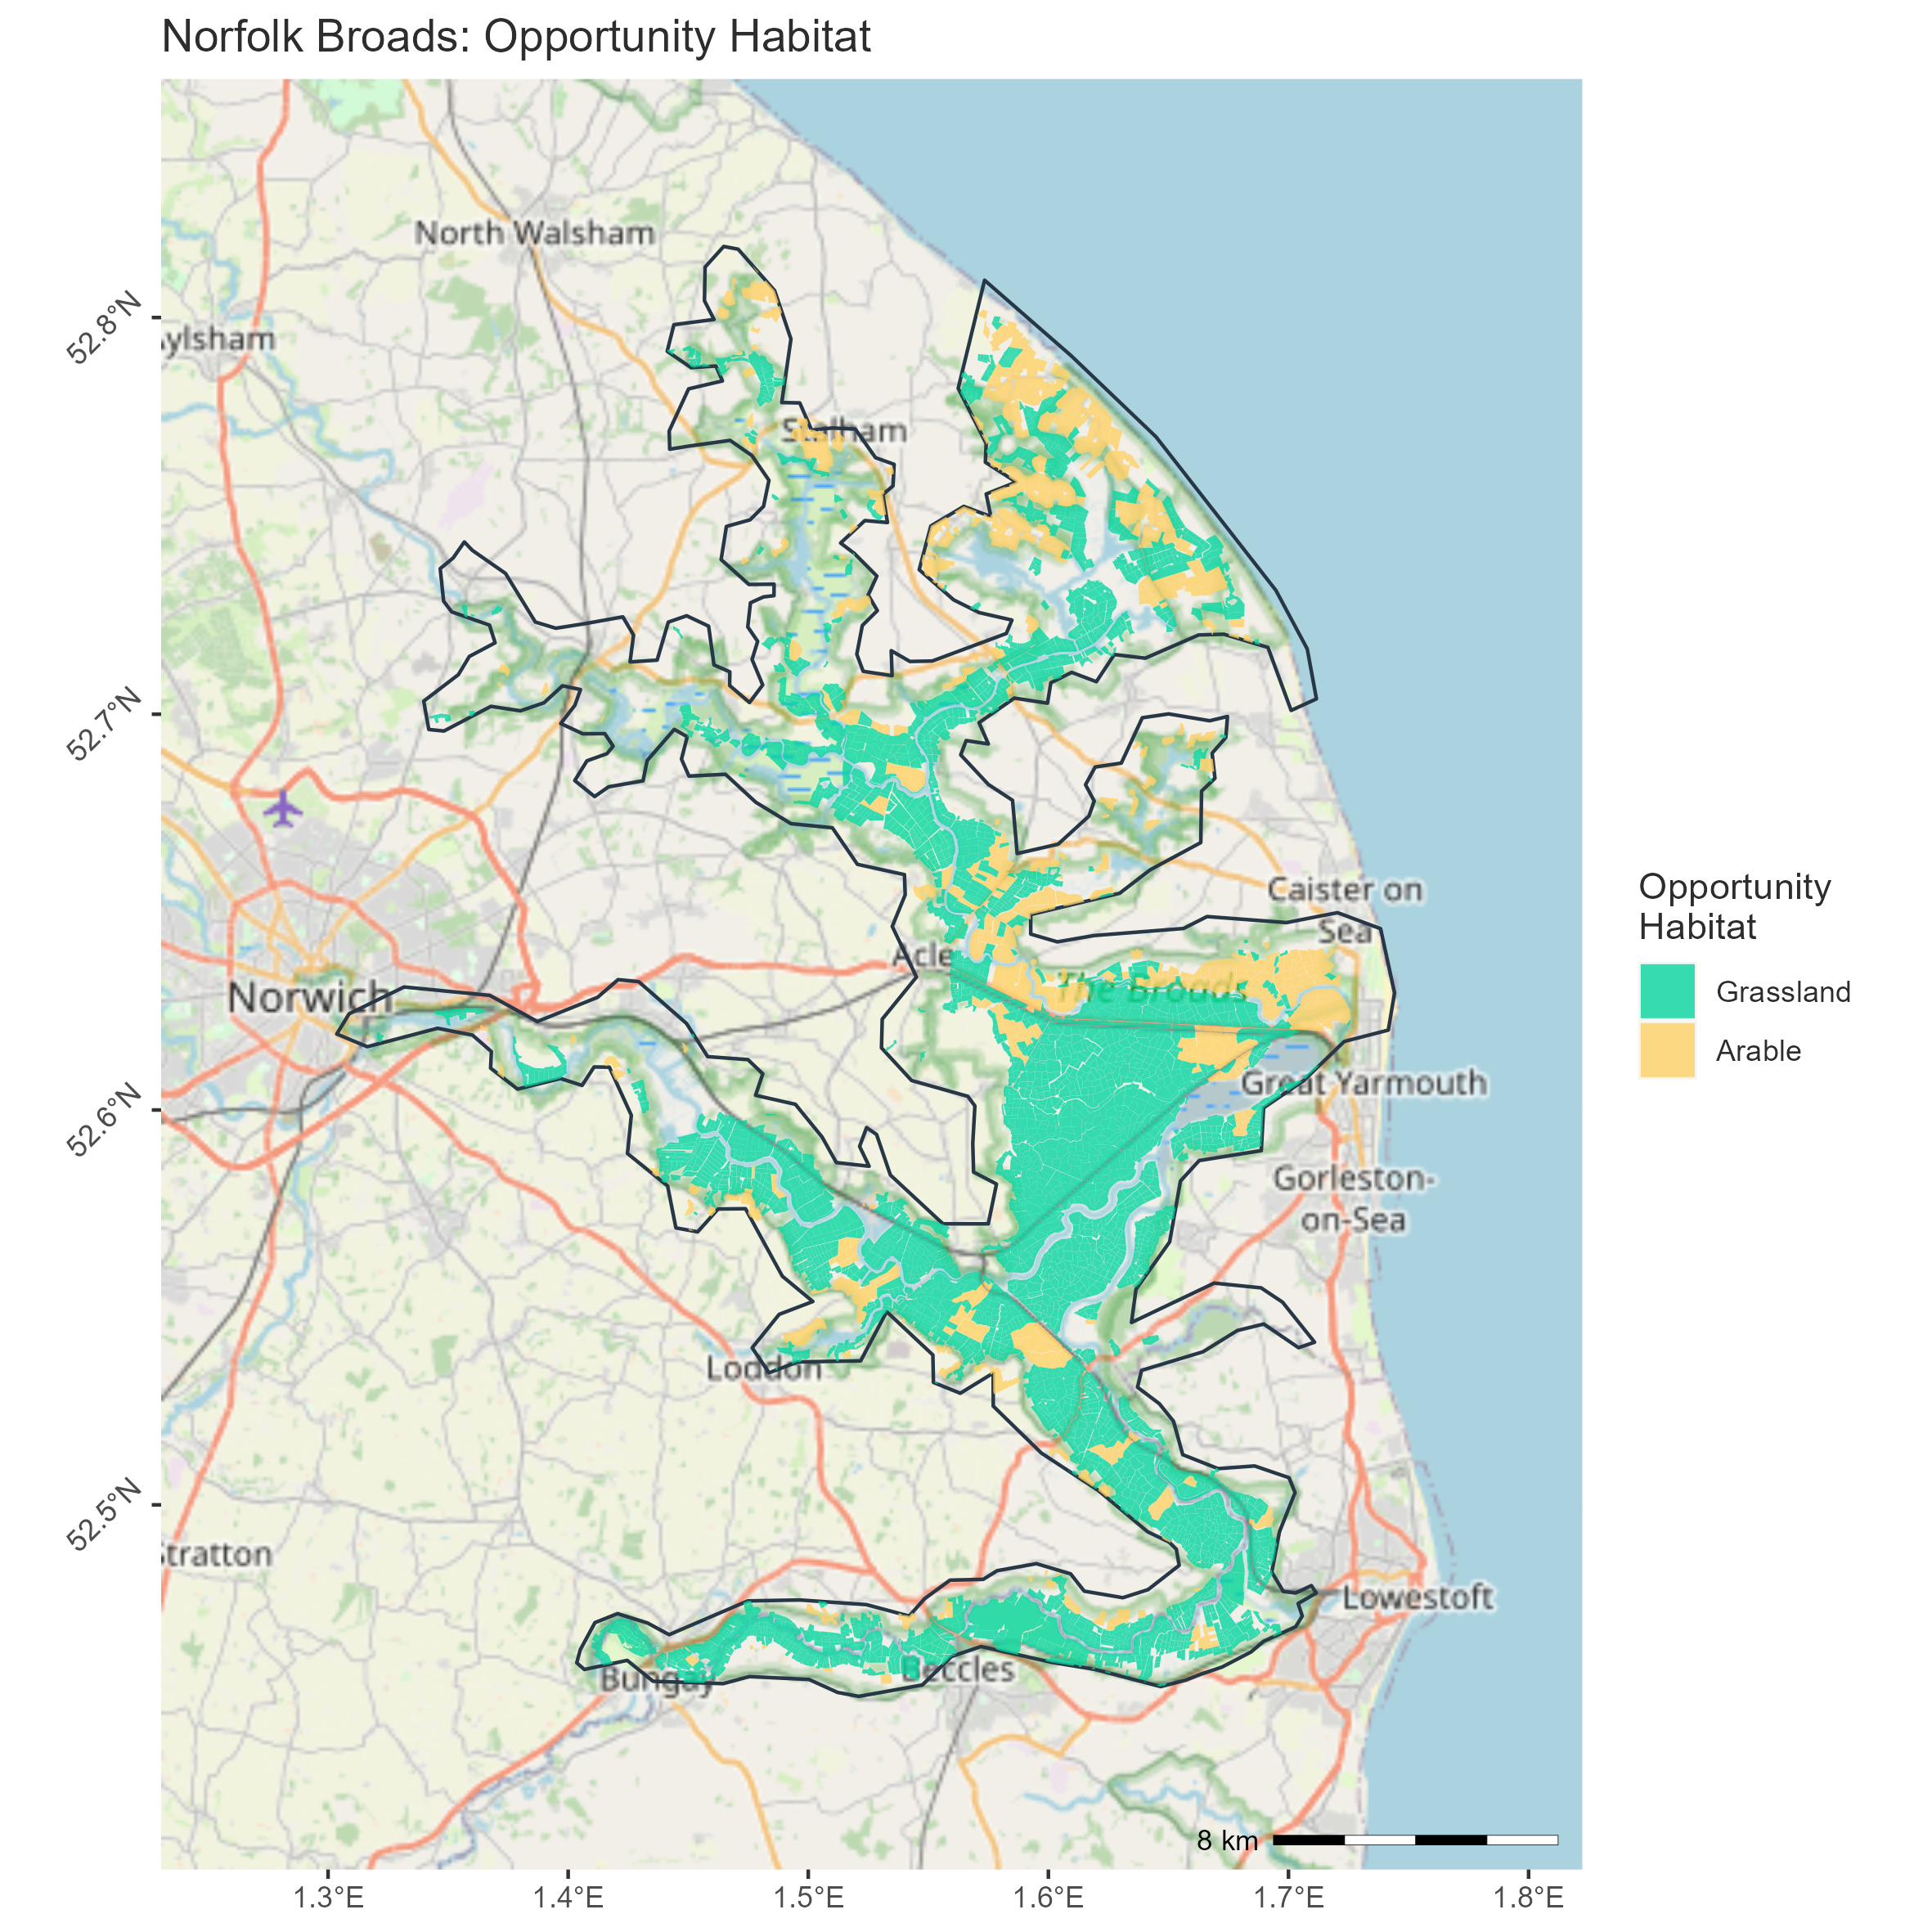
\includegraphics[width=6.25in,height=\textheight]{Plots/Broads_OpportunityHabitatMap.png}

}

\caption{\label{fig-BroadsSuitHab}Parcels in the Norfolk Broads that we
identified as having the right, soil types and elevation to become
lowland wet grassland, regardless of current condition. An OS map is
used as the background.}

\end{figure}%

\begin{figure}[H]

\centering{

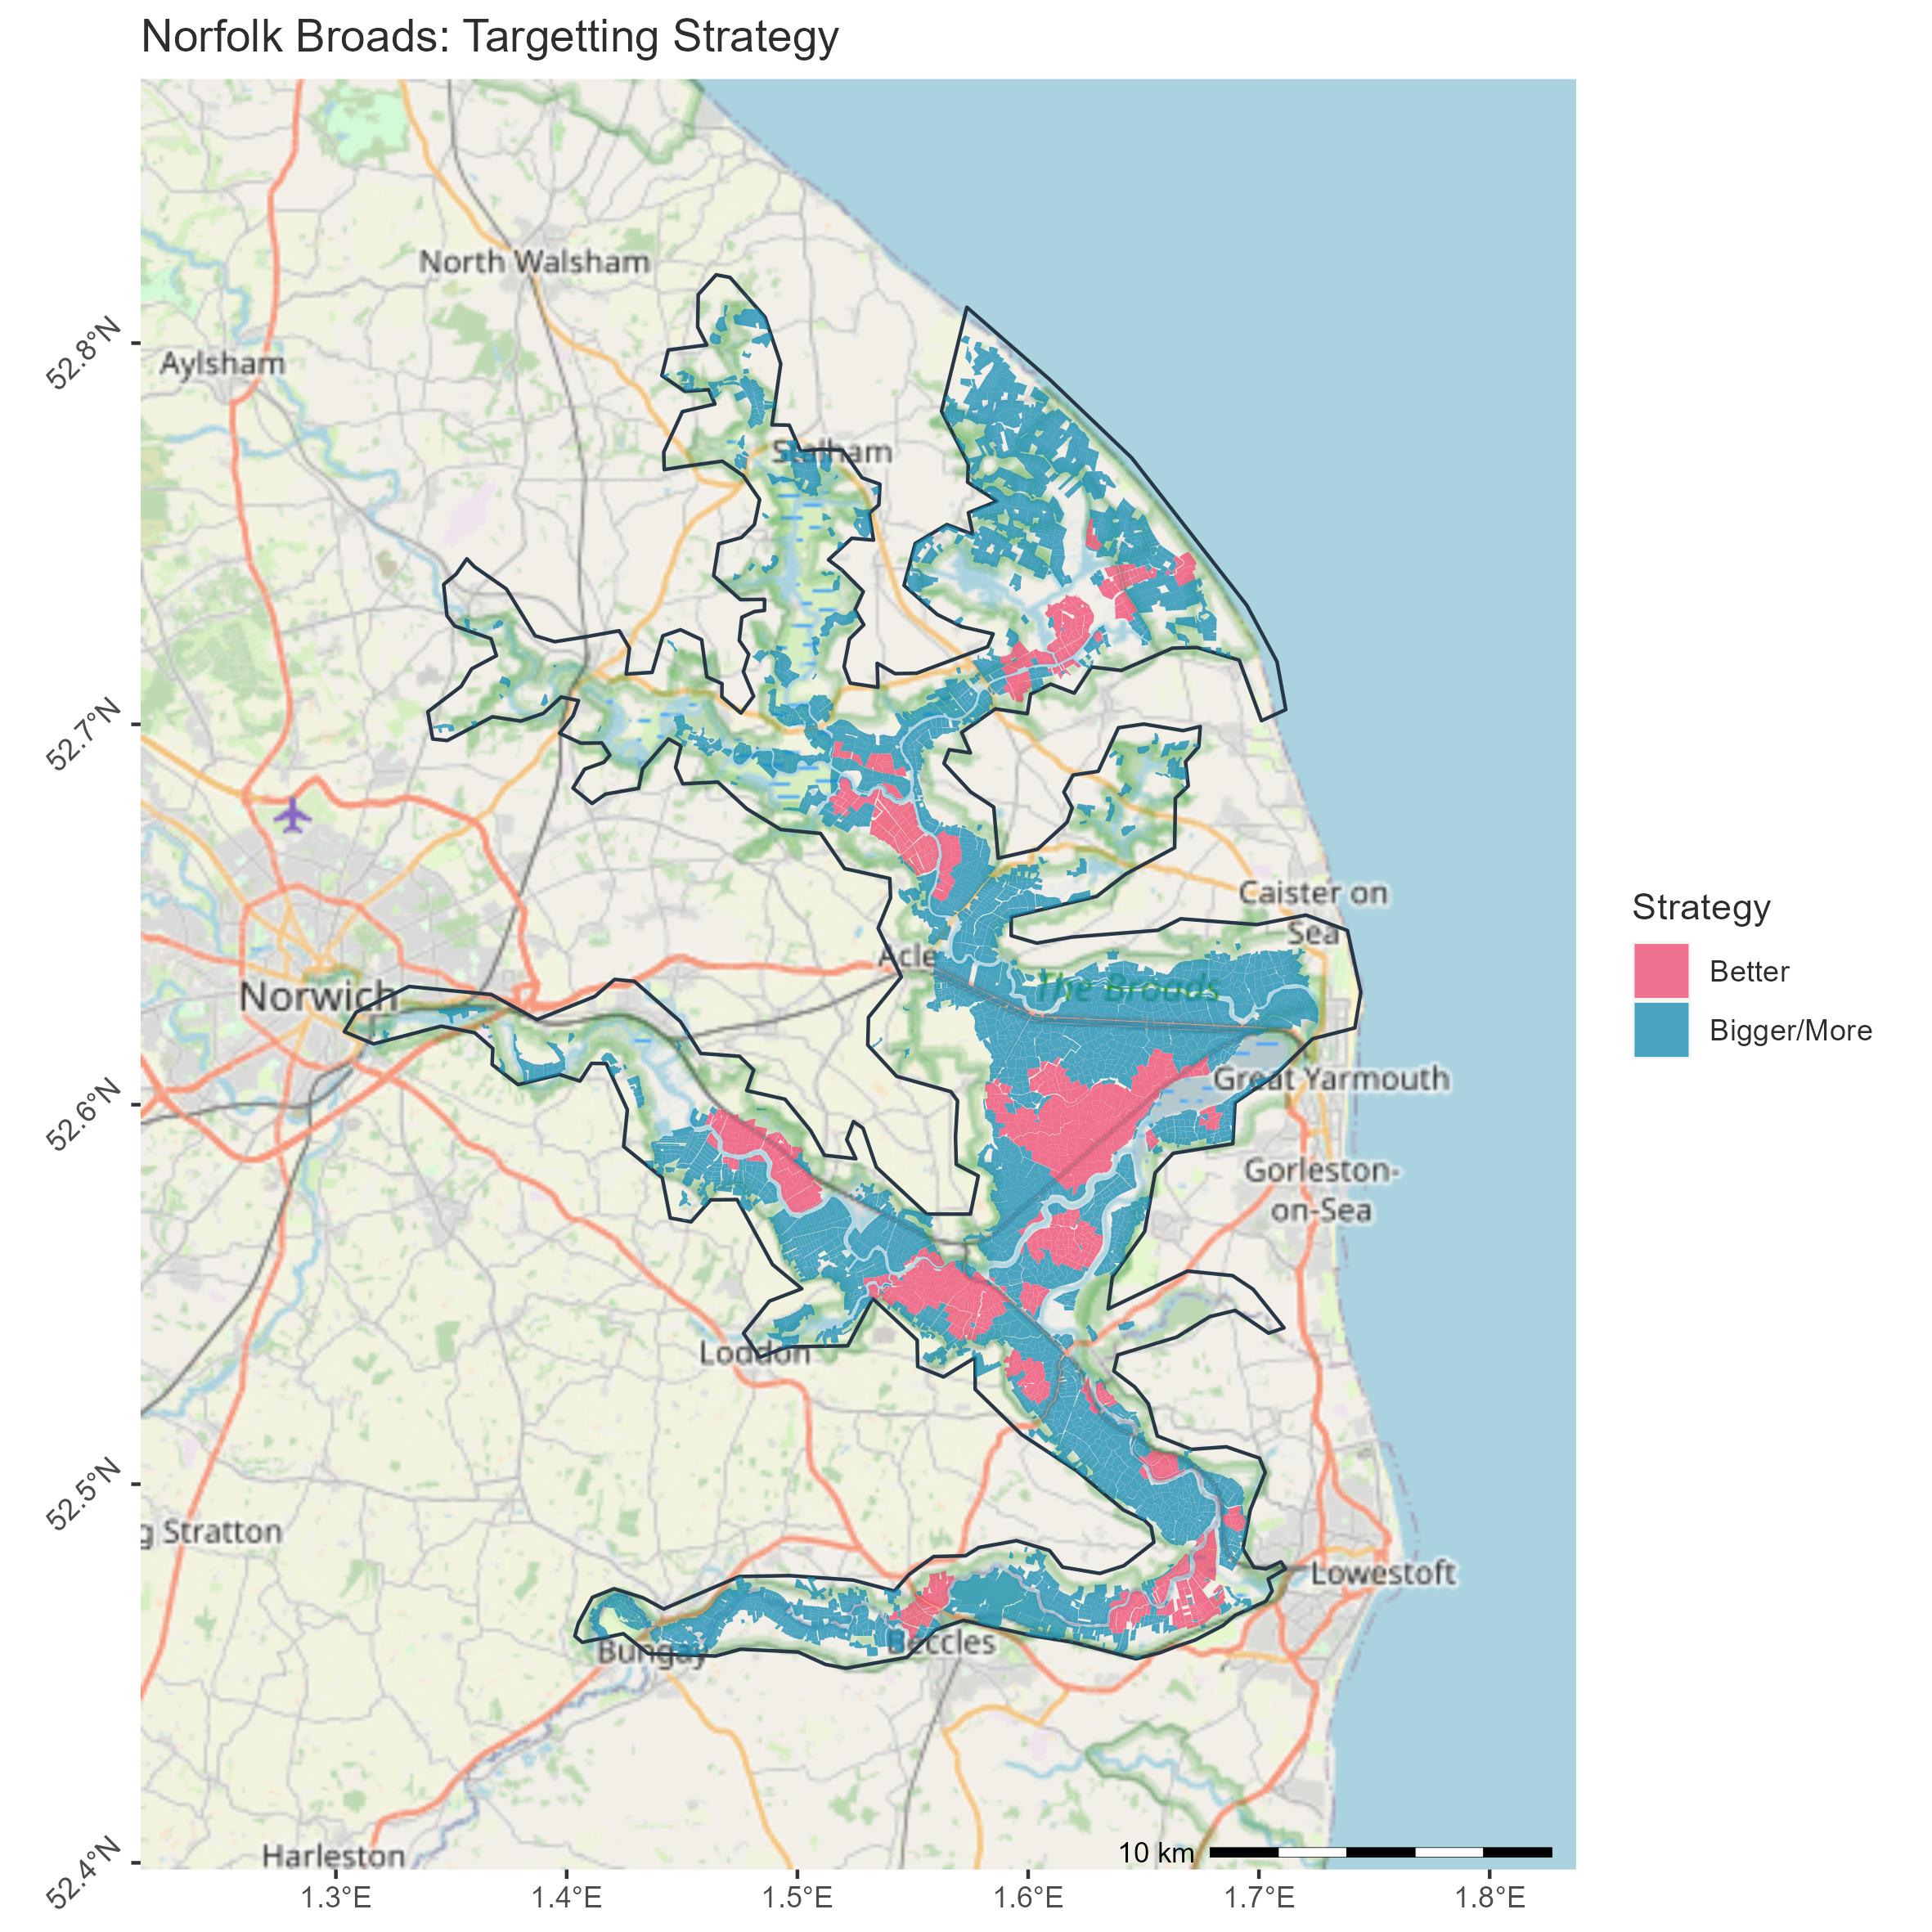
\includegraphics[width=\textwidth,height=9.375in]{Plots/Broads_LawtonPrincipleMap.png}

}

\caption{\label{fig-BroadsLawton}Parcels in the Norfolk Broads that we
identified as being with or outside of lowland breeding wader clusters
in the Norfolk Broads. Tehse clusters were identified using the breeding
waders of wet meadows survey data from 2021-23.}

\end{figure}%

\paragraph{Norfolk Broads: Better}\label{norfolk-broads-better}

The stakeholder preferences for the better principle of nature
restoration for group 1 and group 2 can be visualized in
(Figure~\ref{fig-BroadsBetterG1}) and (Figure~\ref{fig-BroadsBetterG2}),
receptively.

\begin{figure}[H]

\centering{

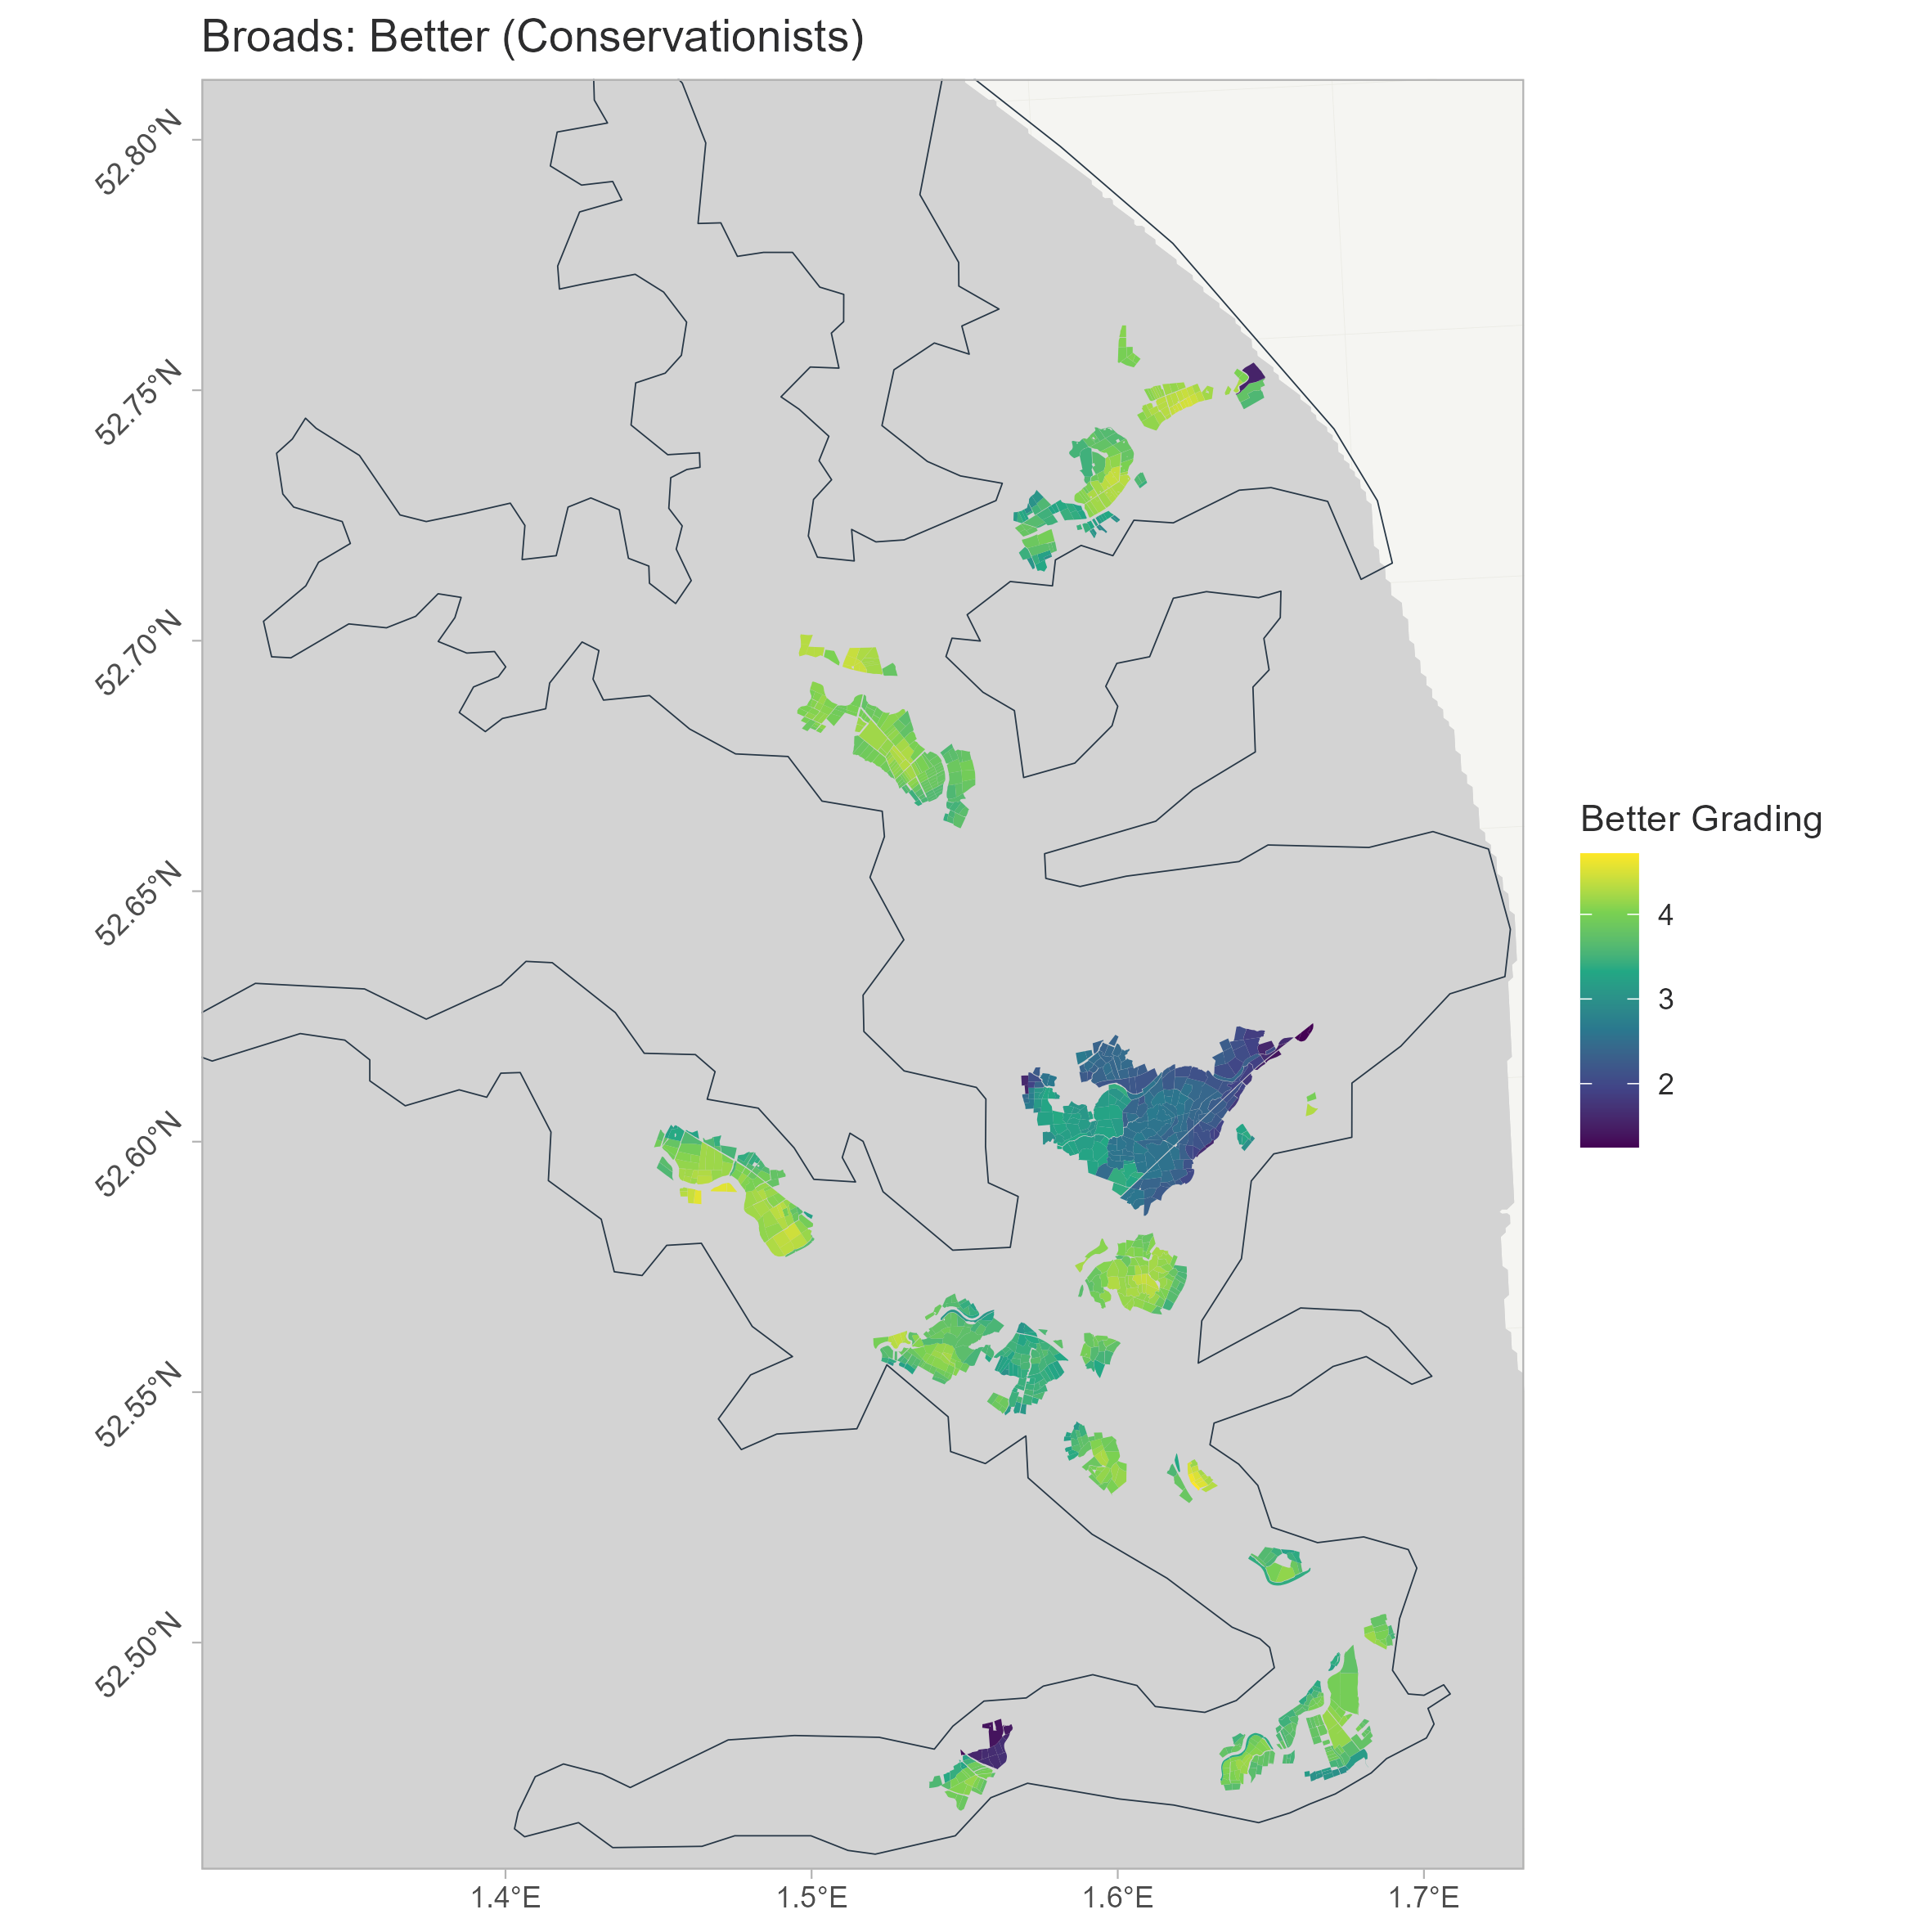
\includegraphics[width=\textwidth,height=10.9375in]{Plots/Broads_G1_Better.png}

}

\caption{\label{fig-BroadsBetterG1}Stakeholder gradings for group 1 in
the Norfolk Broads for the better principle of nature restoration}

\end{figure}%

\begin{figure}[H]

\centering{

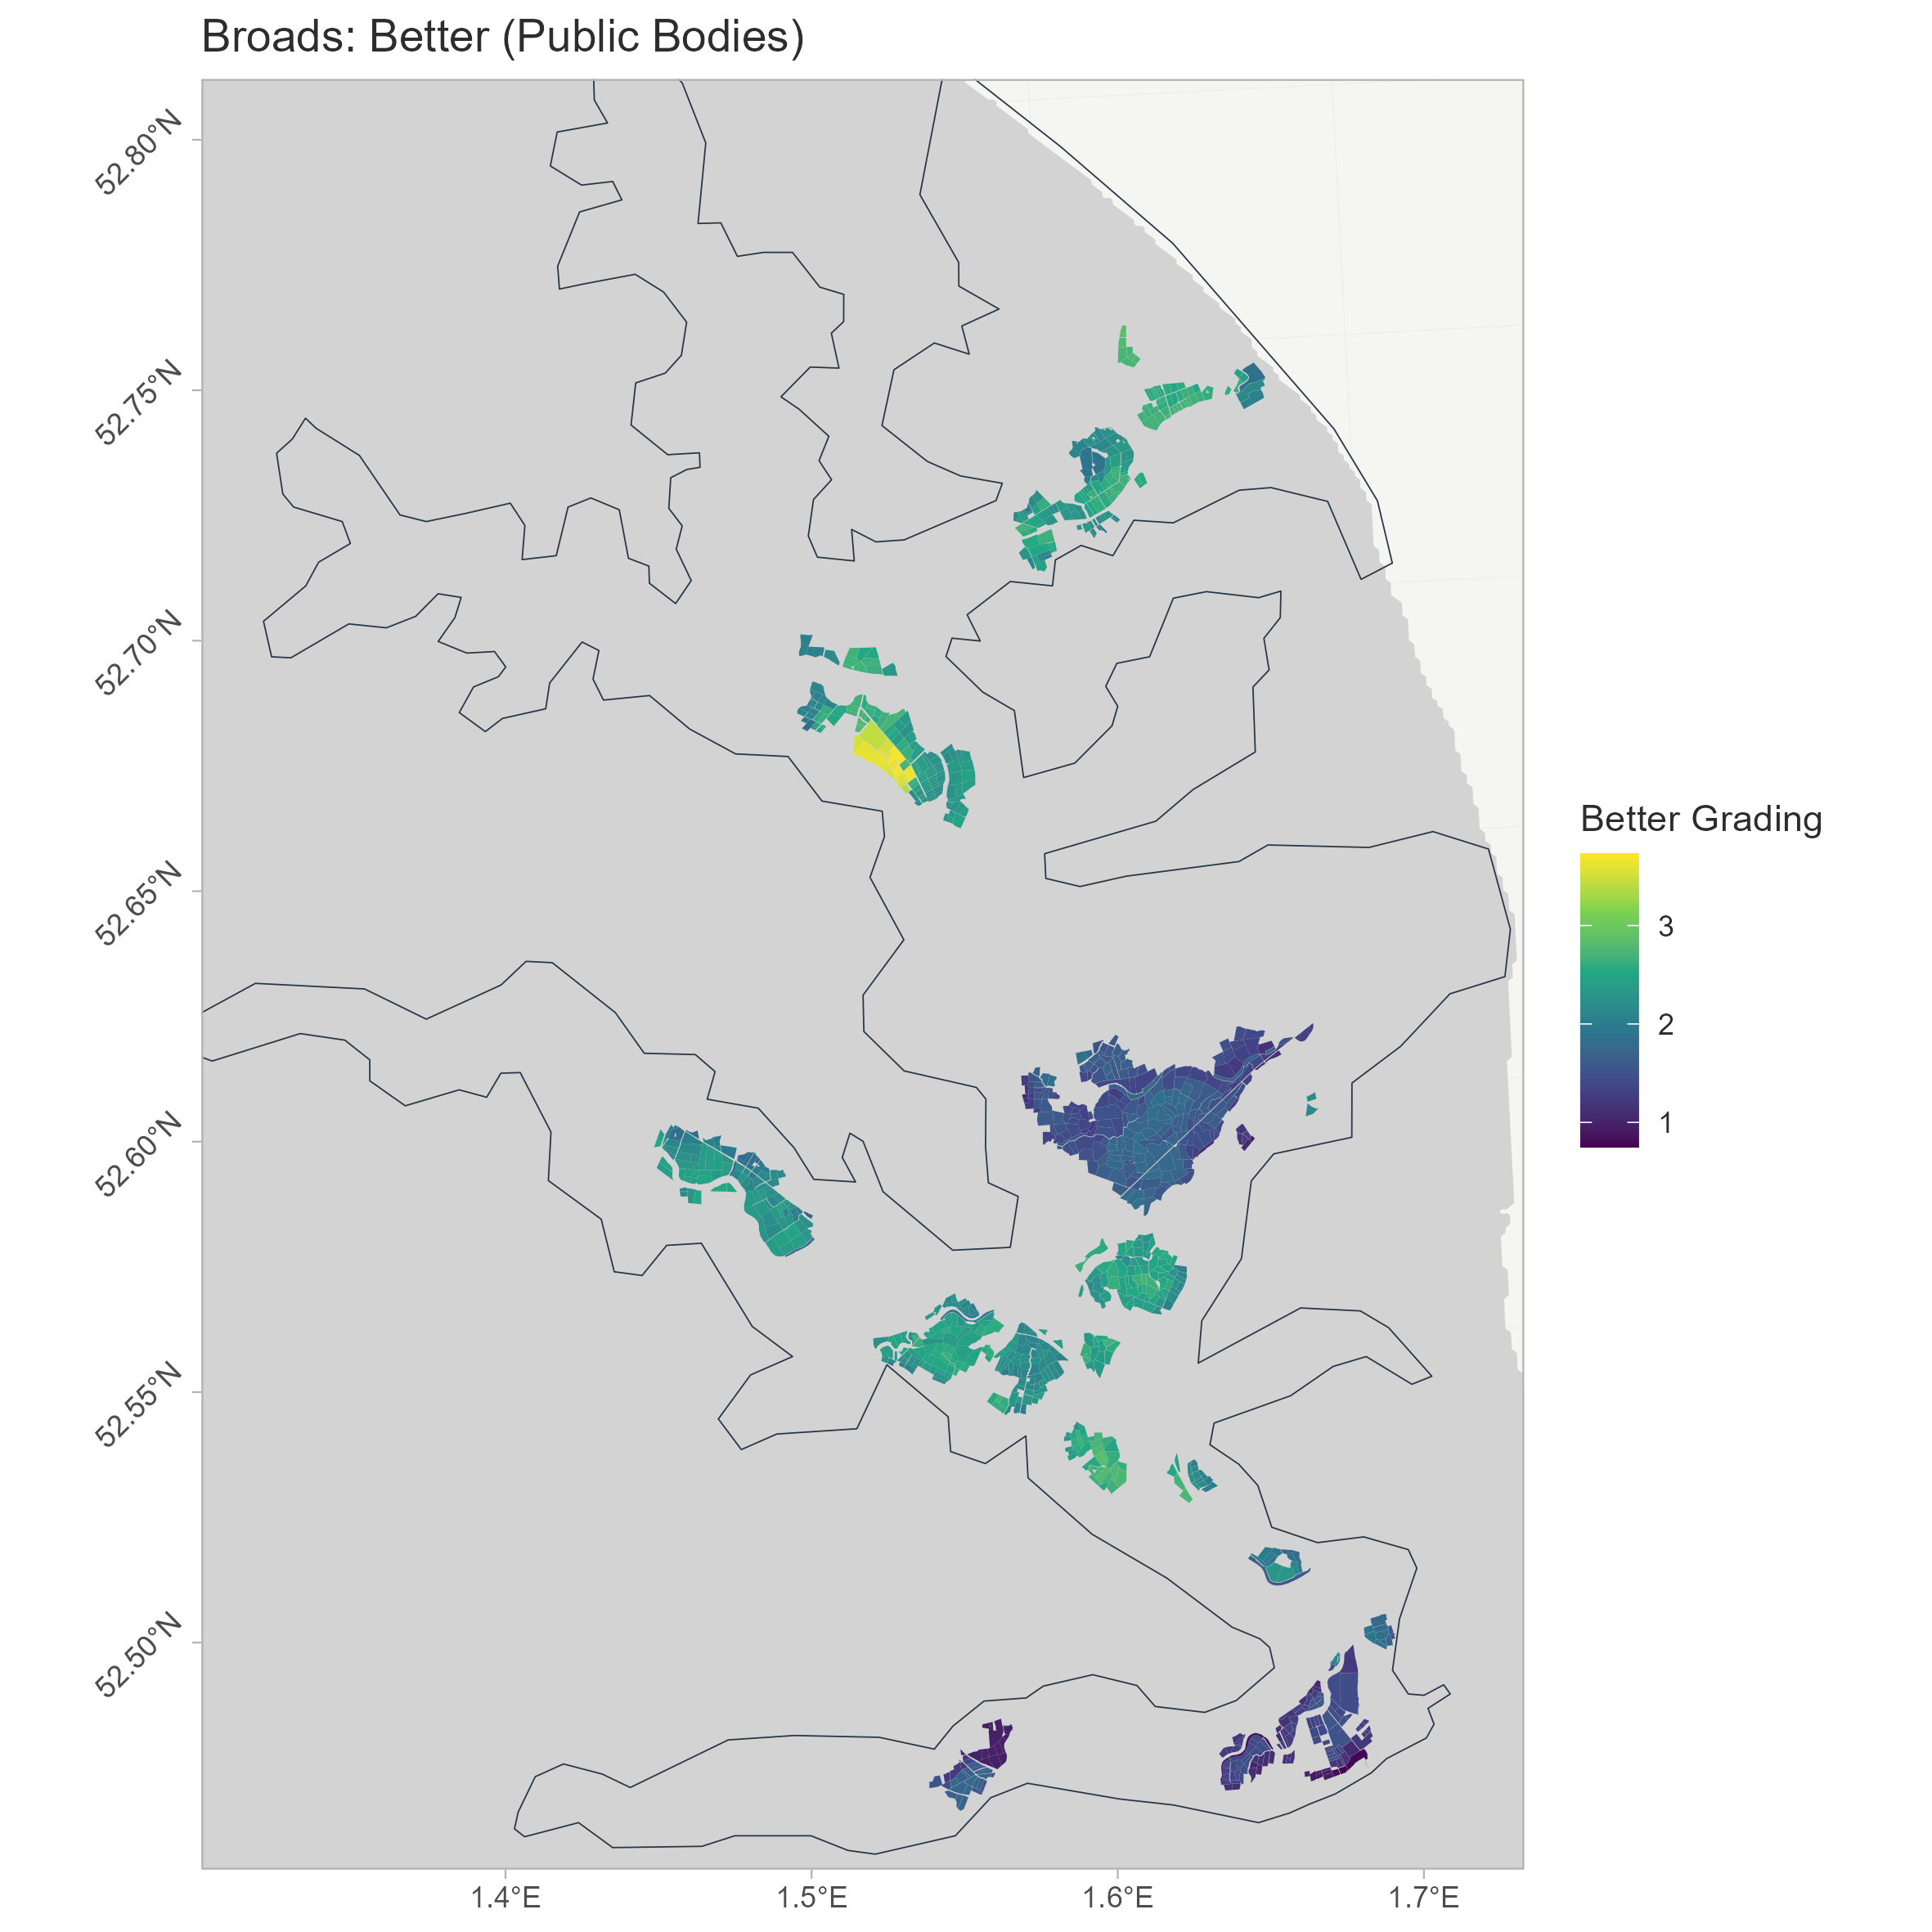
\includegraphics[width=\textwidth,height=10.41667in]{Plots/Broads_G2_Better.png}

}

\caption{\label{fig-BroadsBetterG2}Stakeholder gradings for group 2 in
the Norfolk Broads for the better principle of nature restoration}

\end{figure}%

\newpage{}

\paragraph{Norfolk Broads: Bigger}\label{norfolk-broads-bigger}

The stakeholder preferences for the bigger principle of nature
restoration for group 1 (Figure~\ref{fig-BroadsBigG1}) and 2
(Figure~\ref{fig-BroadsBigG2}).

\begin{figure}[H]

\centering{

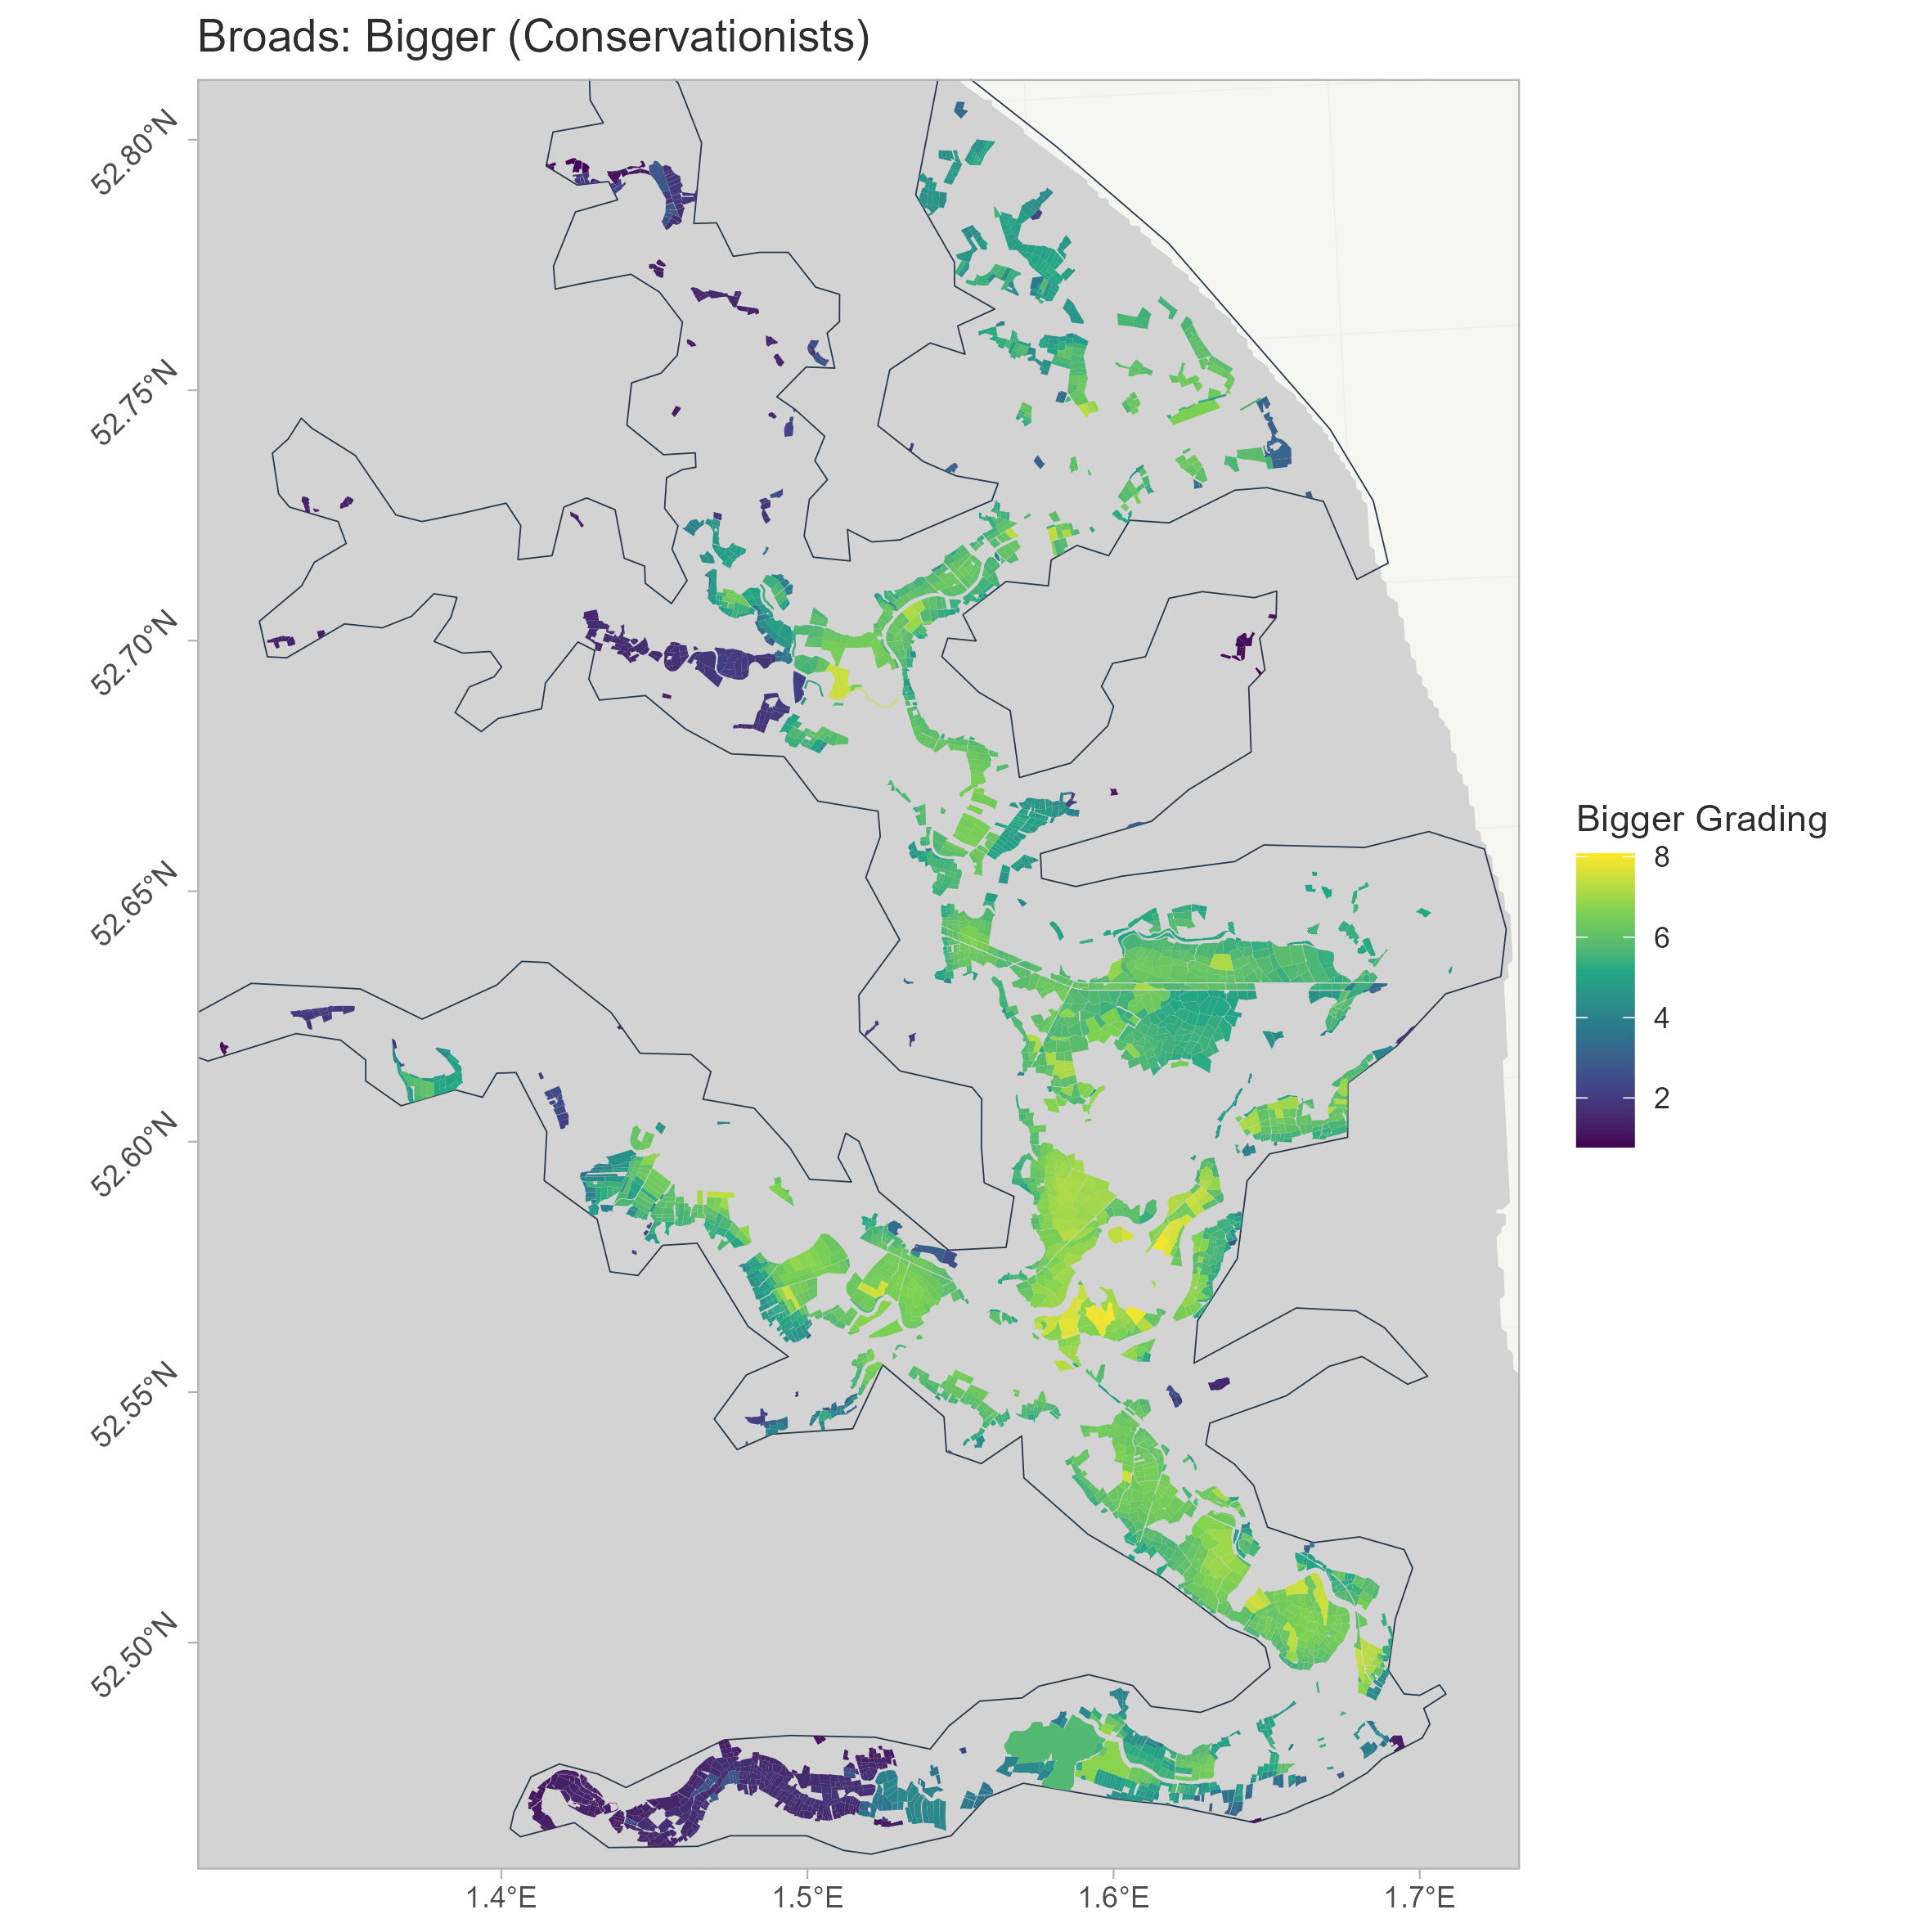
\includegraphics[width=\textwidth,height=9.89583in]{Plots/Broads_G1_Bigger.png}

}

\caption{\label{fig-BroadsBigG1}Stakeholder gradings for group 1 in the
Norfolk Broads for the bigger principle of nature restoration}

\end{figure}%

\begin{figure}[H]

\centering{

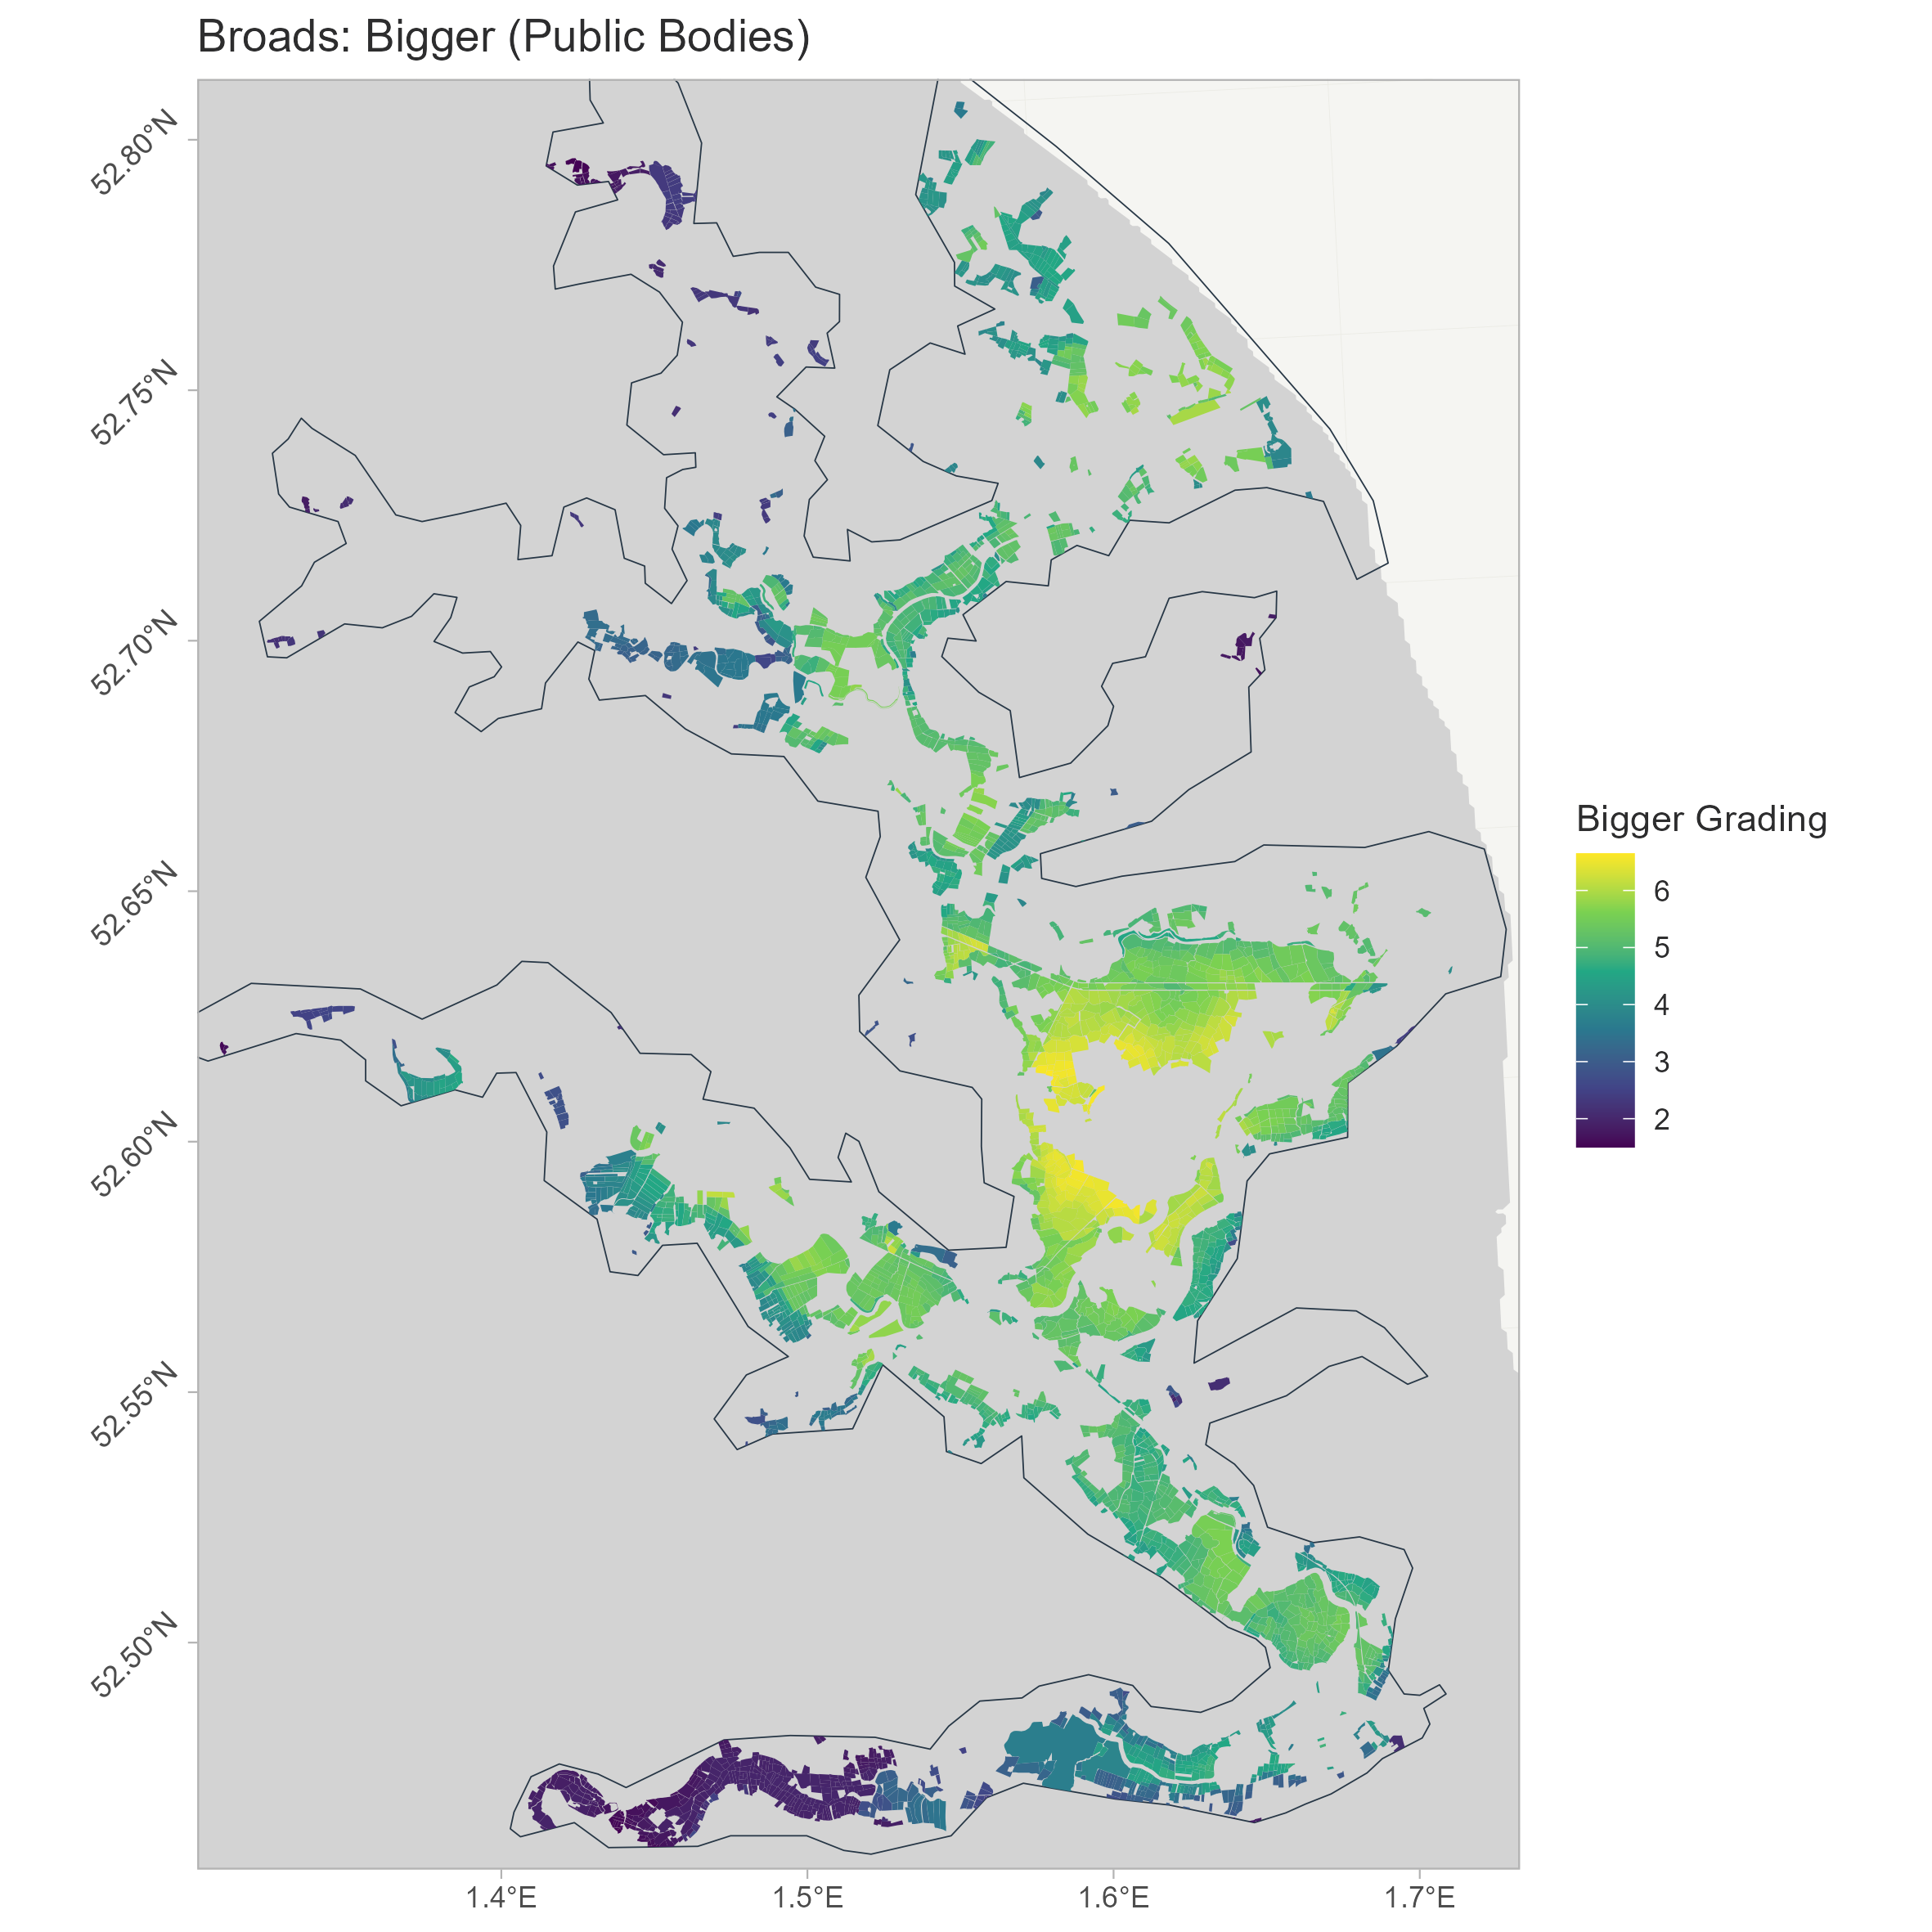
\includegraphics[width=\textwidth,height=9.375in]{Plots/Broads_G2_Bigger.png}

}

\caption{\label{fig-BroadsBigG2}Stakeholder gradings for group 2 in the
Norfolk Broads for the bigger principle of nature restoration}

\end{figure}%

\newpage{}

\paragraph{Norfolk Broads: More}\label{norfolk-broads-more}

The stakeholder preferences for the more principle of nature restoration
for group 1 (Figure~\ref{fig-BroadsMoreG1}) and 2
(Figure~\ref{fig-BroadsMoreG2}).

\begin{figure}[H]

\centering{

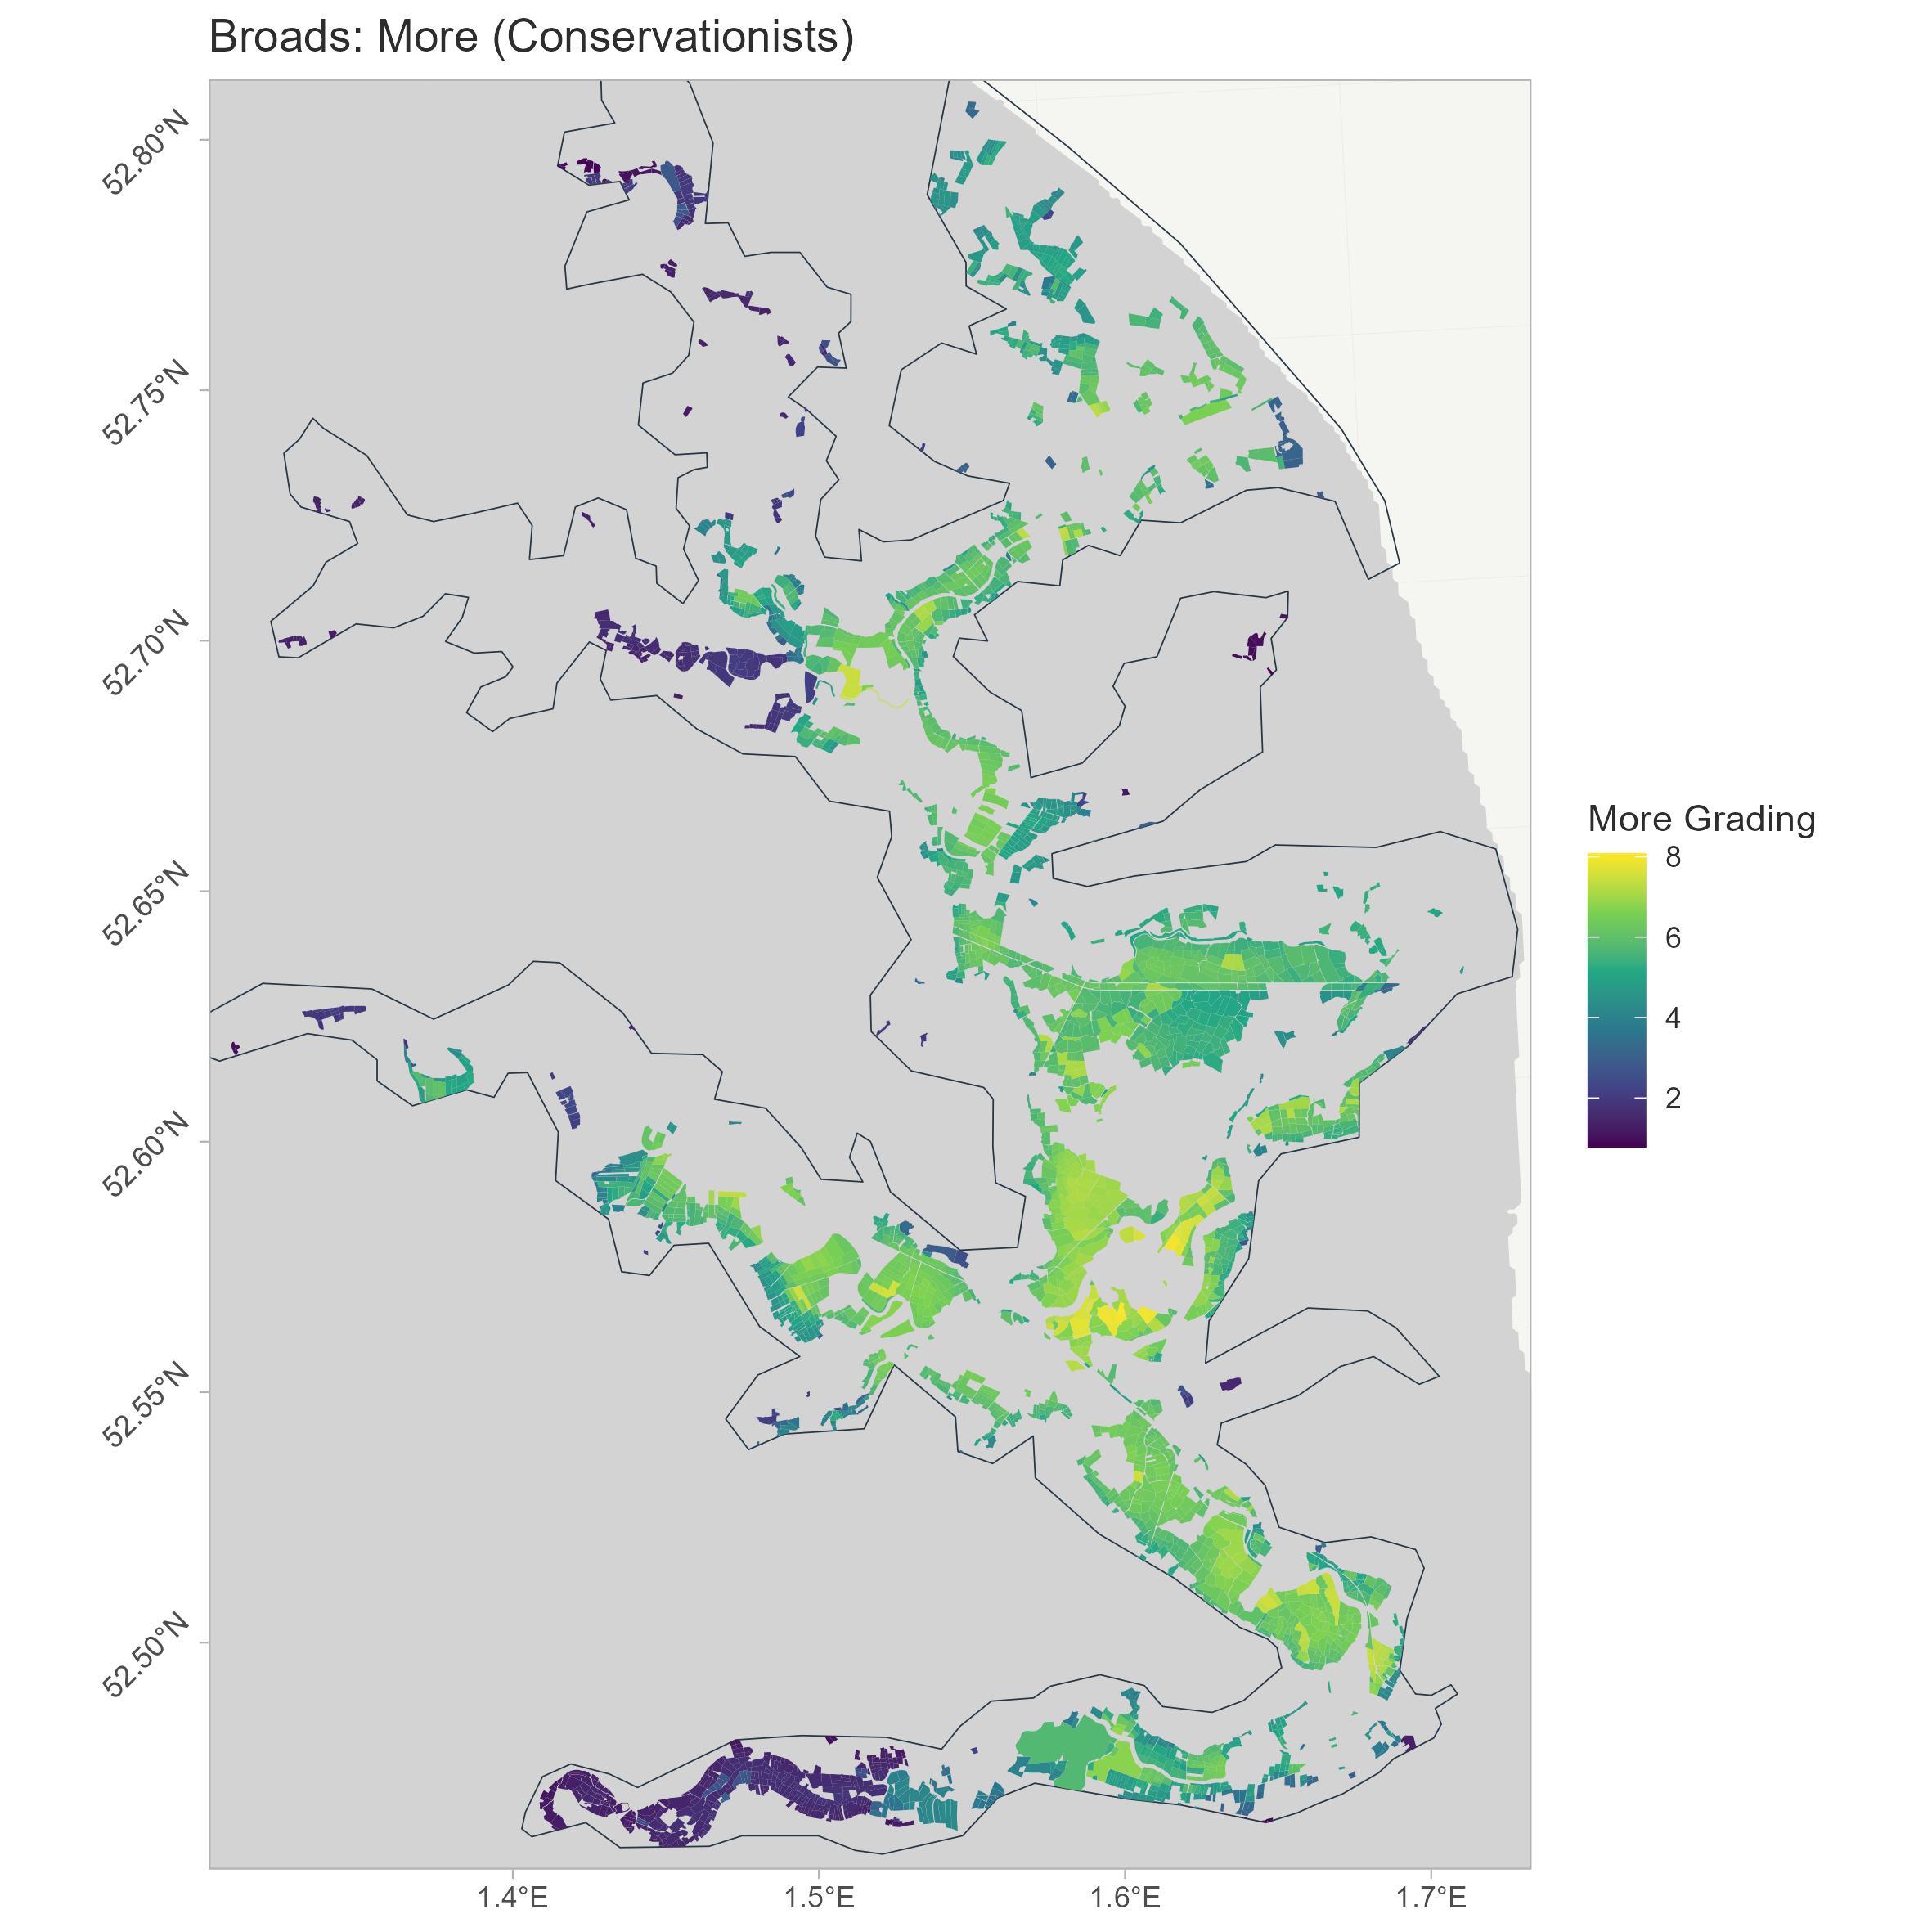
\includegraphics[width=\textwidth,height=9.375in]{Plots/Broads_G1_More.png}

}

\caption{\label{fig-BroadsMoreG1}Stakeholder gradings for group 1 in the
Norfolk Broads for the more principle of nature restoration}

\end{figure}%

\begin{figure}[H]

\centering{

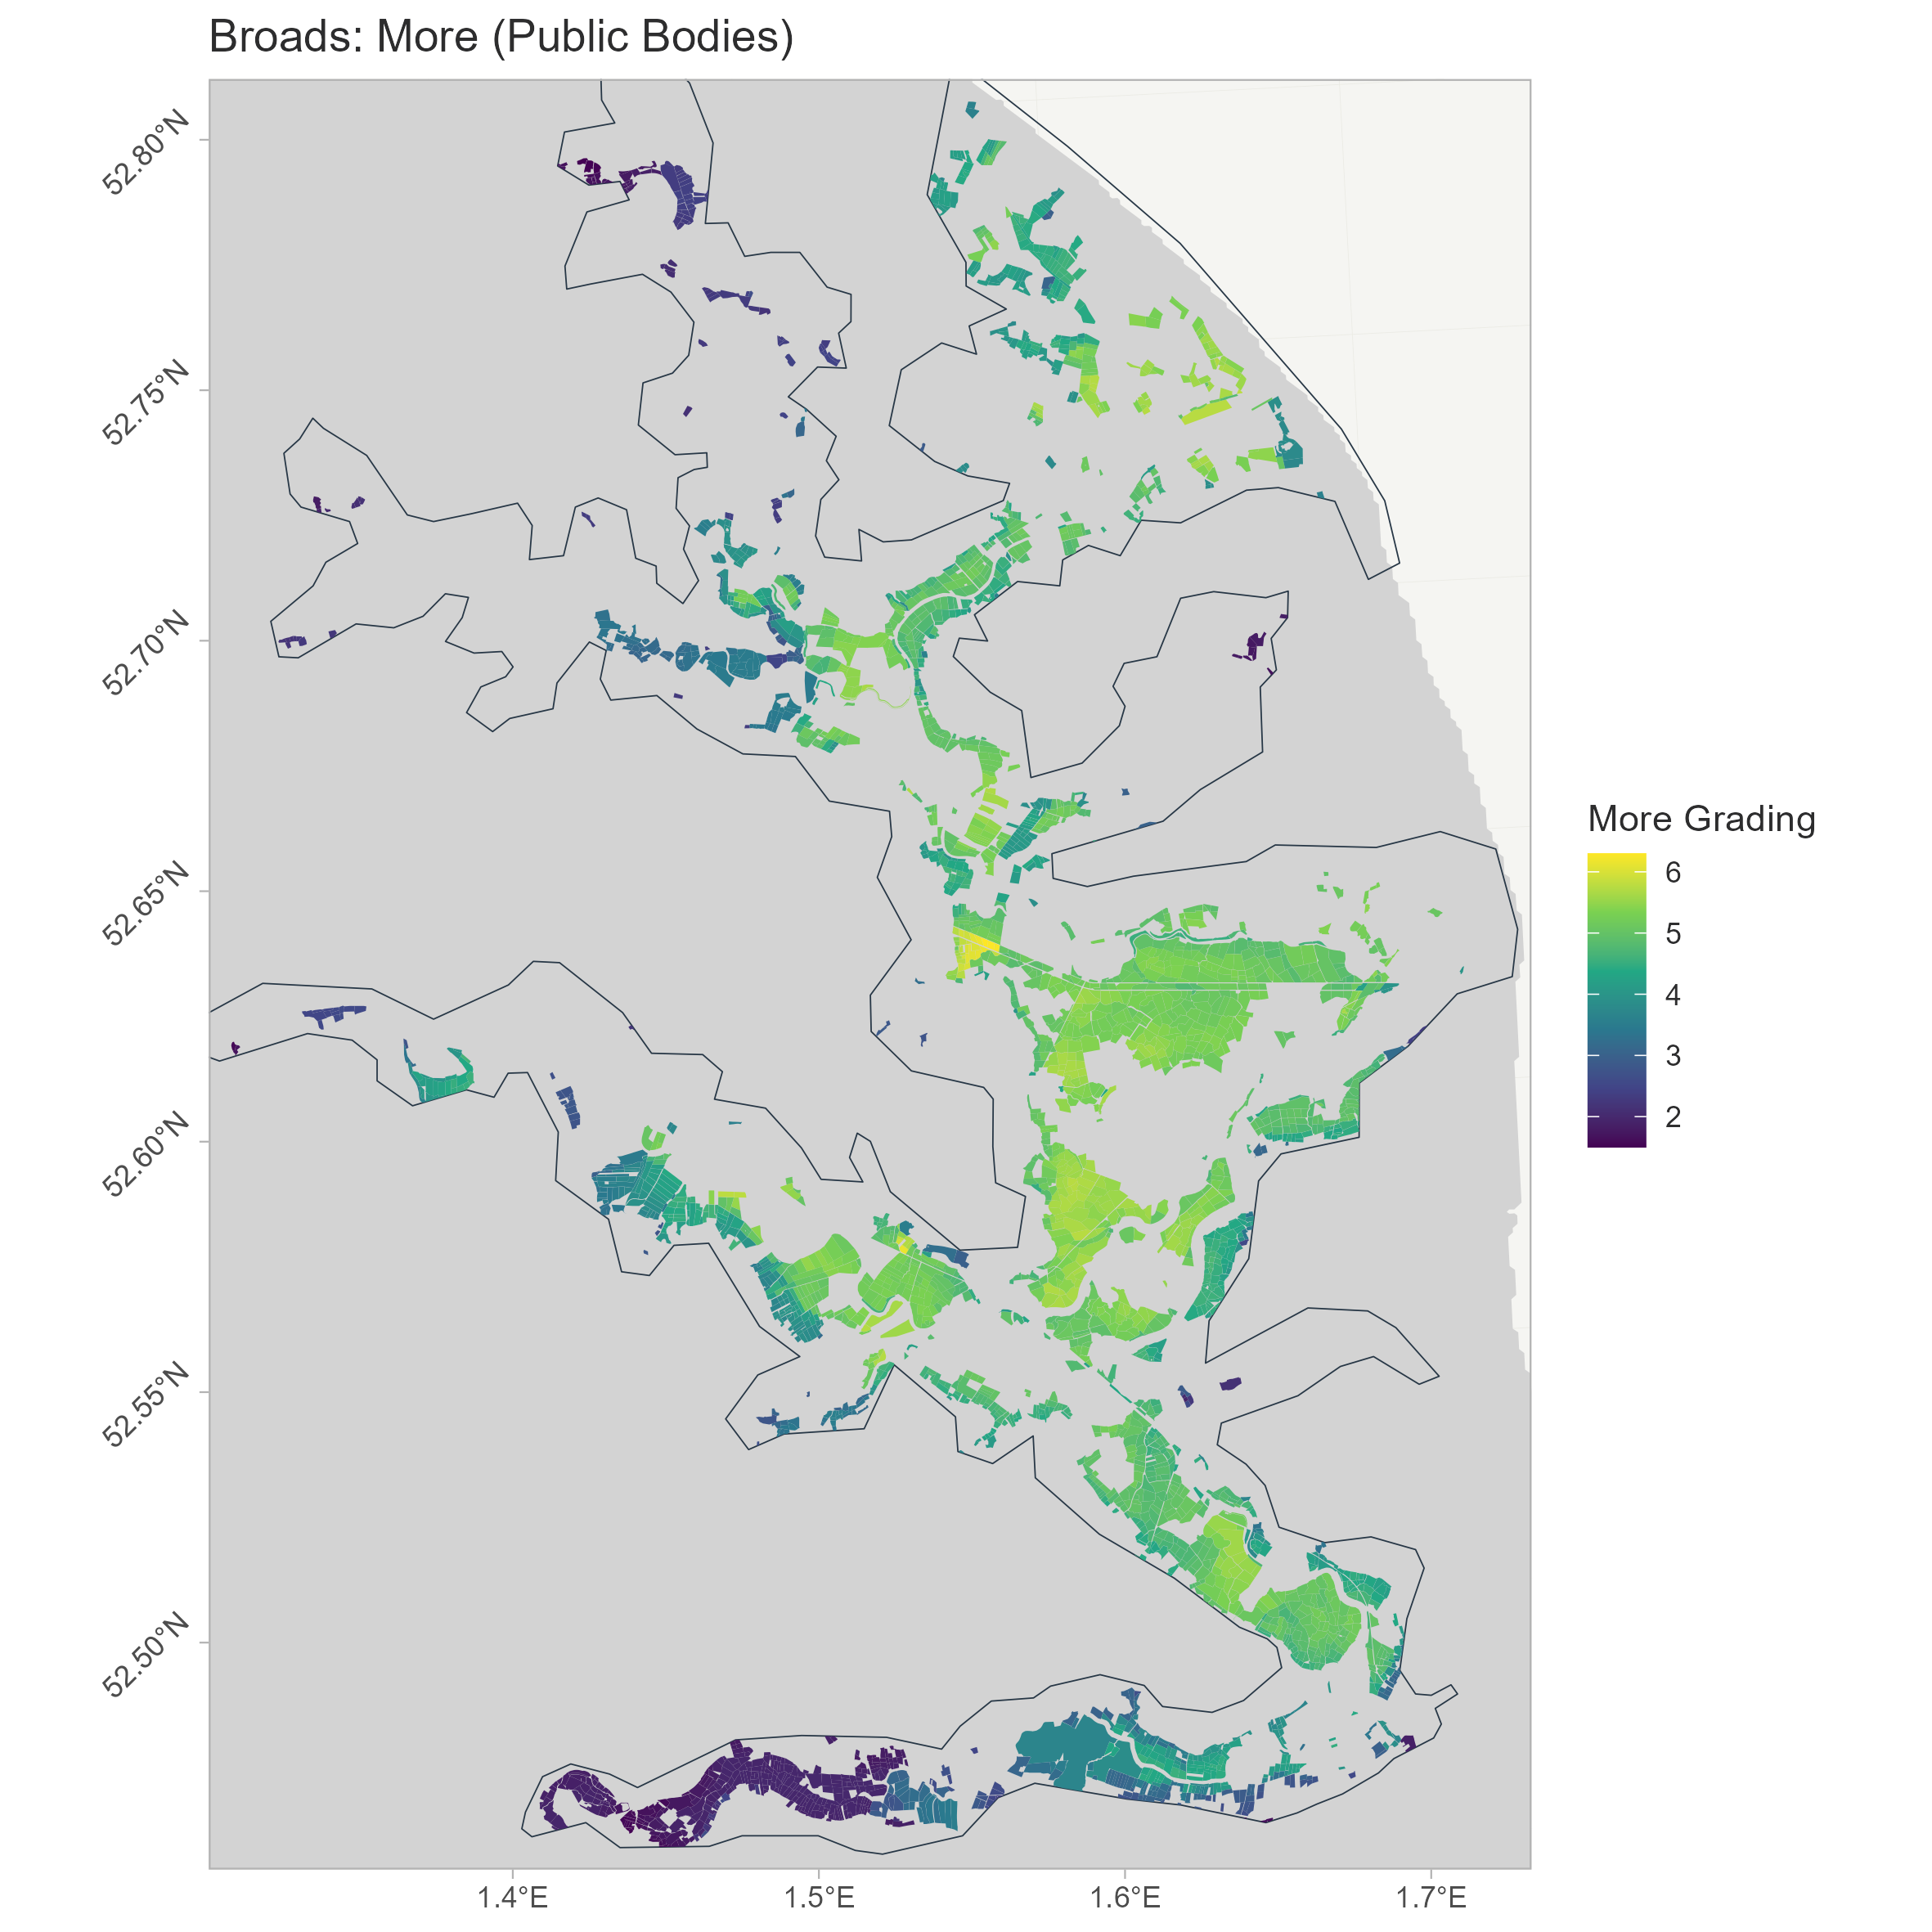
\includegraphics[width=\textwidth,height=9.375in]{Plots/Broads_G2_More.png}

}

\caption{\label{fig-BroadsMoreG2}Stakeholder gradings for group 2 in the
Norfolk Broads for the more principle of nature restoration}

\end{figure}%

\newpage{}

\paragraph{Norfolk Broads: Arable Conversion for
Bigger}\label{norfolk-broads-arable-conversion-for-bigger}

The stakeholder preferences for the conversion of arable land to lowland
wet grassland under the bigger principle of nature restoration for group
1 (Figure~\ref{fig-BroadsArBigG1}) and 2
(Figure~\ref{fig-BroadsArBigG2}).

\begin{figure}[H]

\centering{

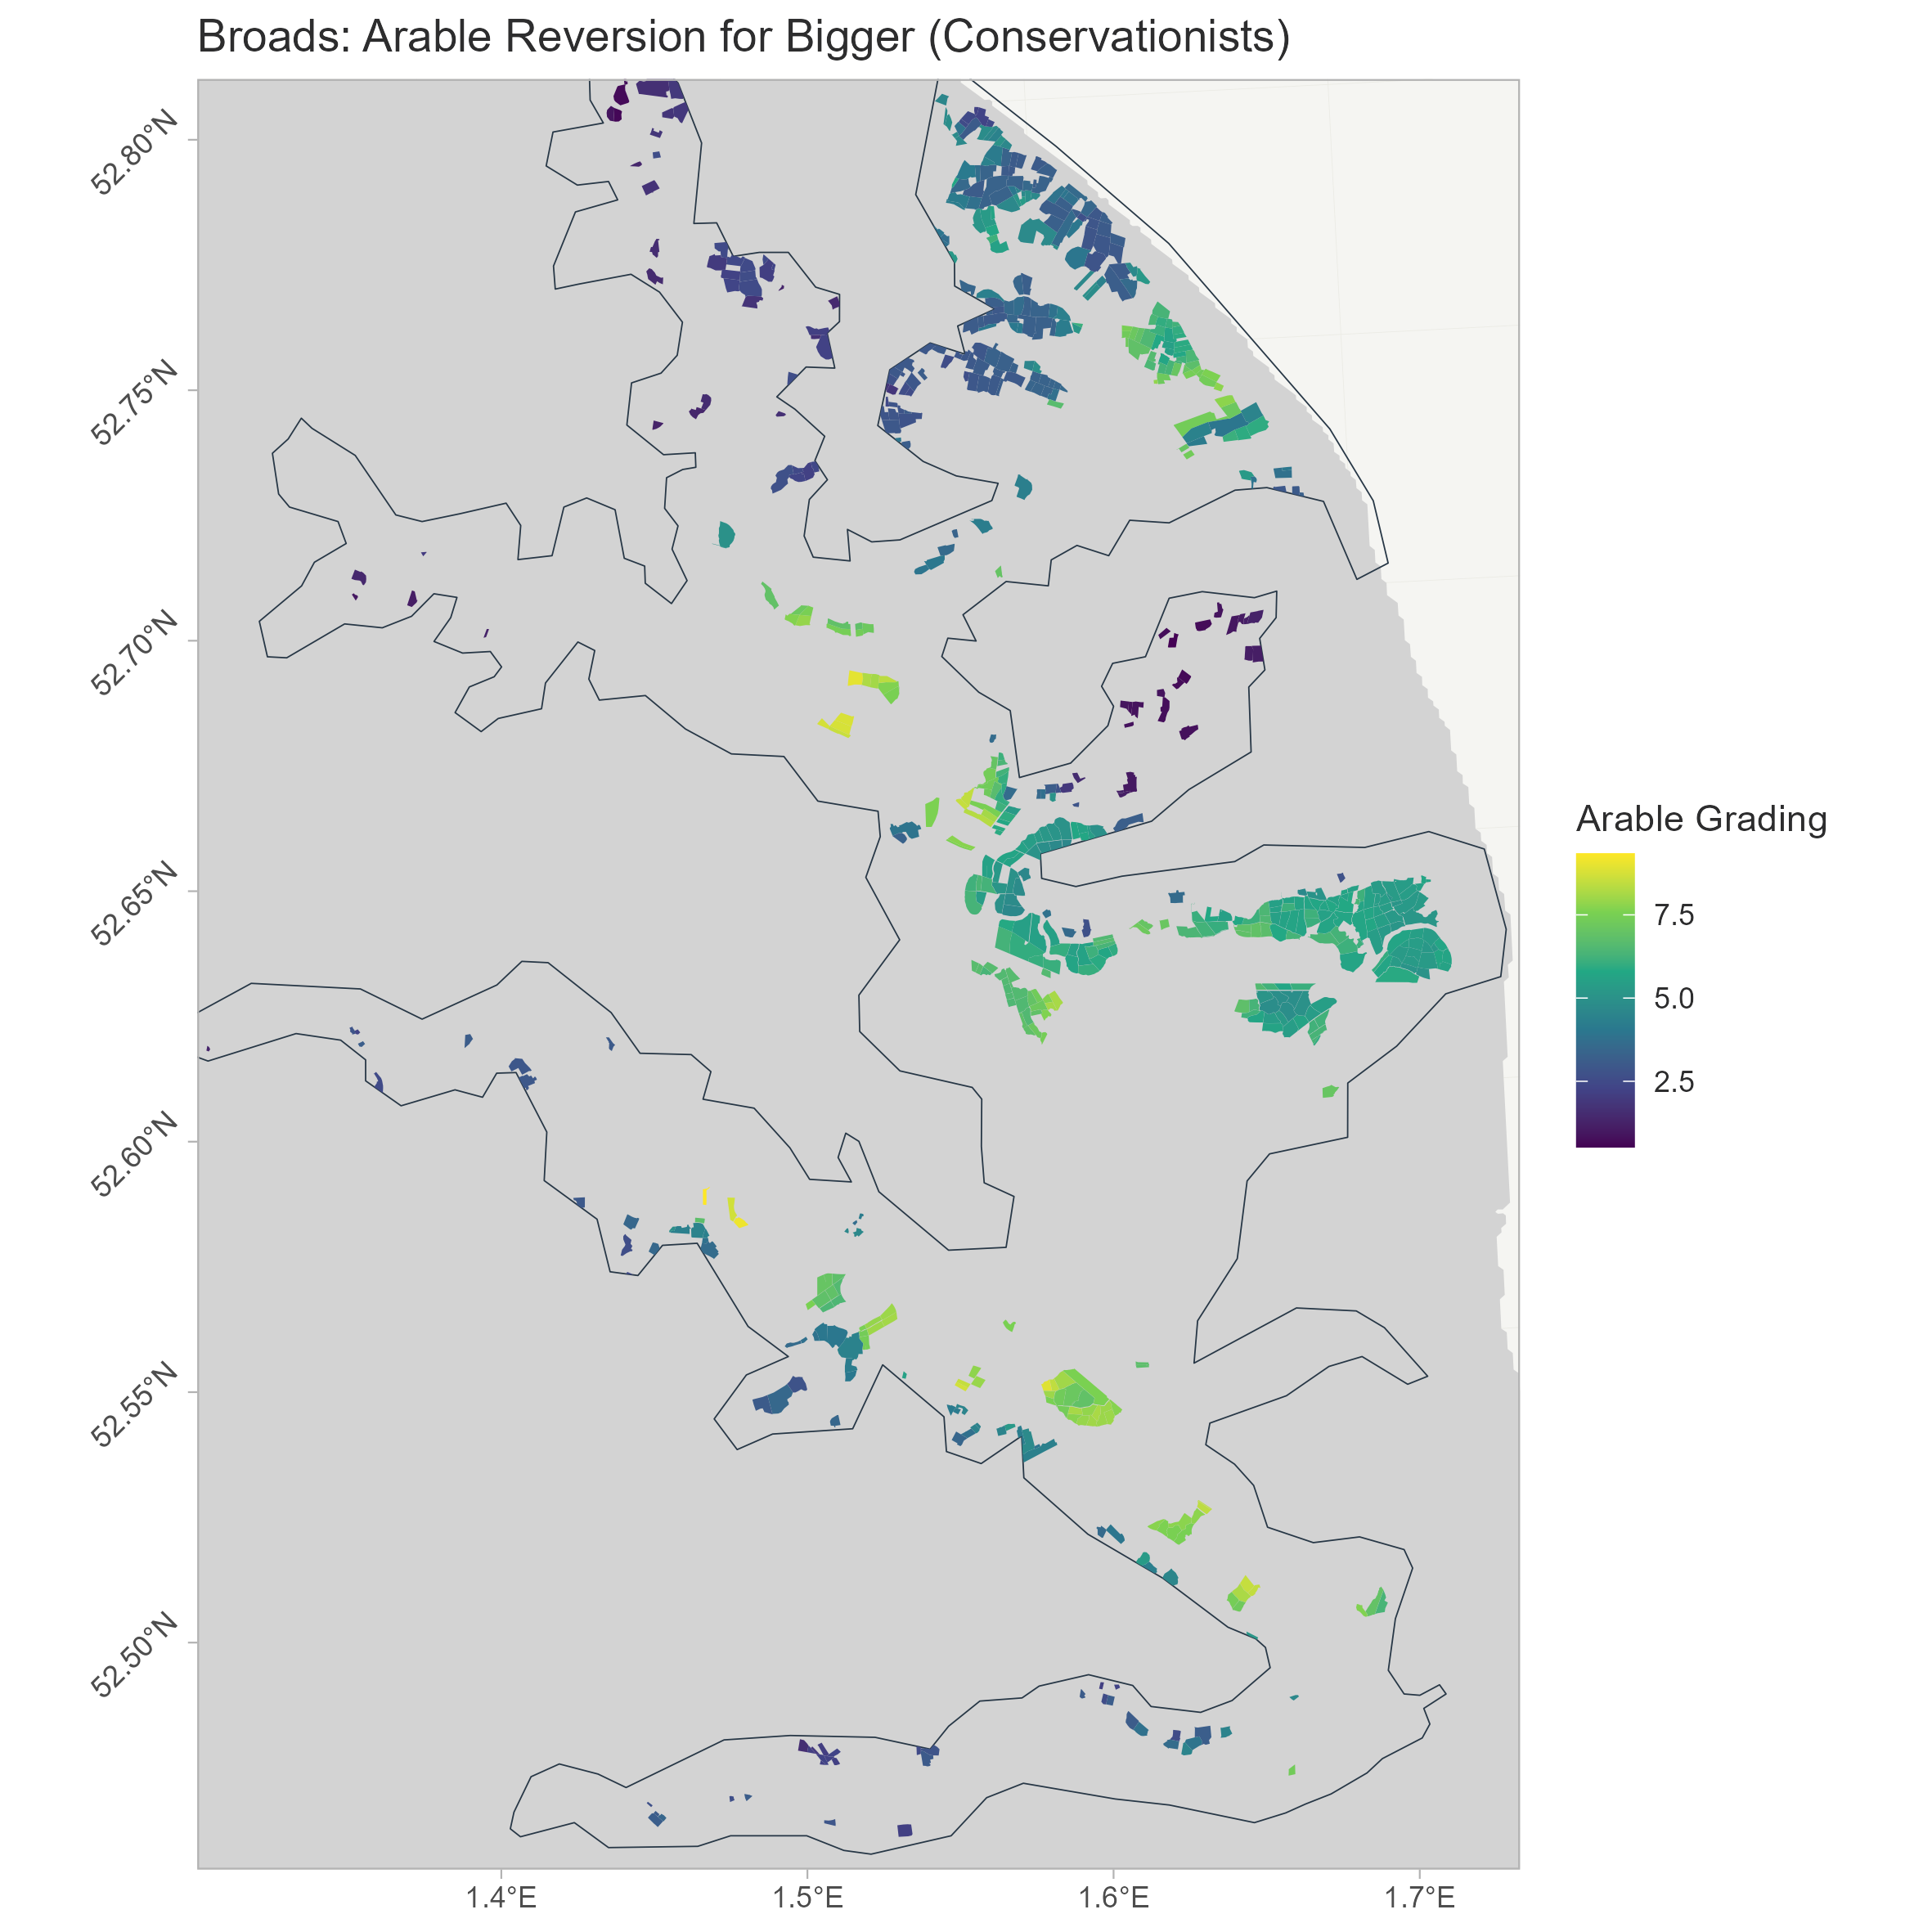
\includegraphics[width=\textwidth,height=9.375in]{Plots/Broads_G1_ArableBig.png}

}

\caption{\label{fig-BroadsArBigG1}Stakeholder gradings for group 1 in
the Norfolk Broads for the reversion of arable land to lowland wet
grassland under the bigger principle of nature restoration}

\end{figure}%

\begin{figure}[H]

\centering{

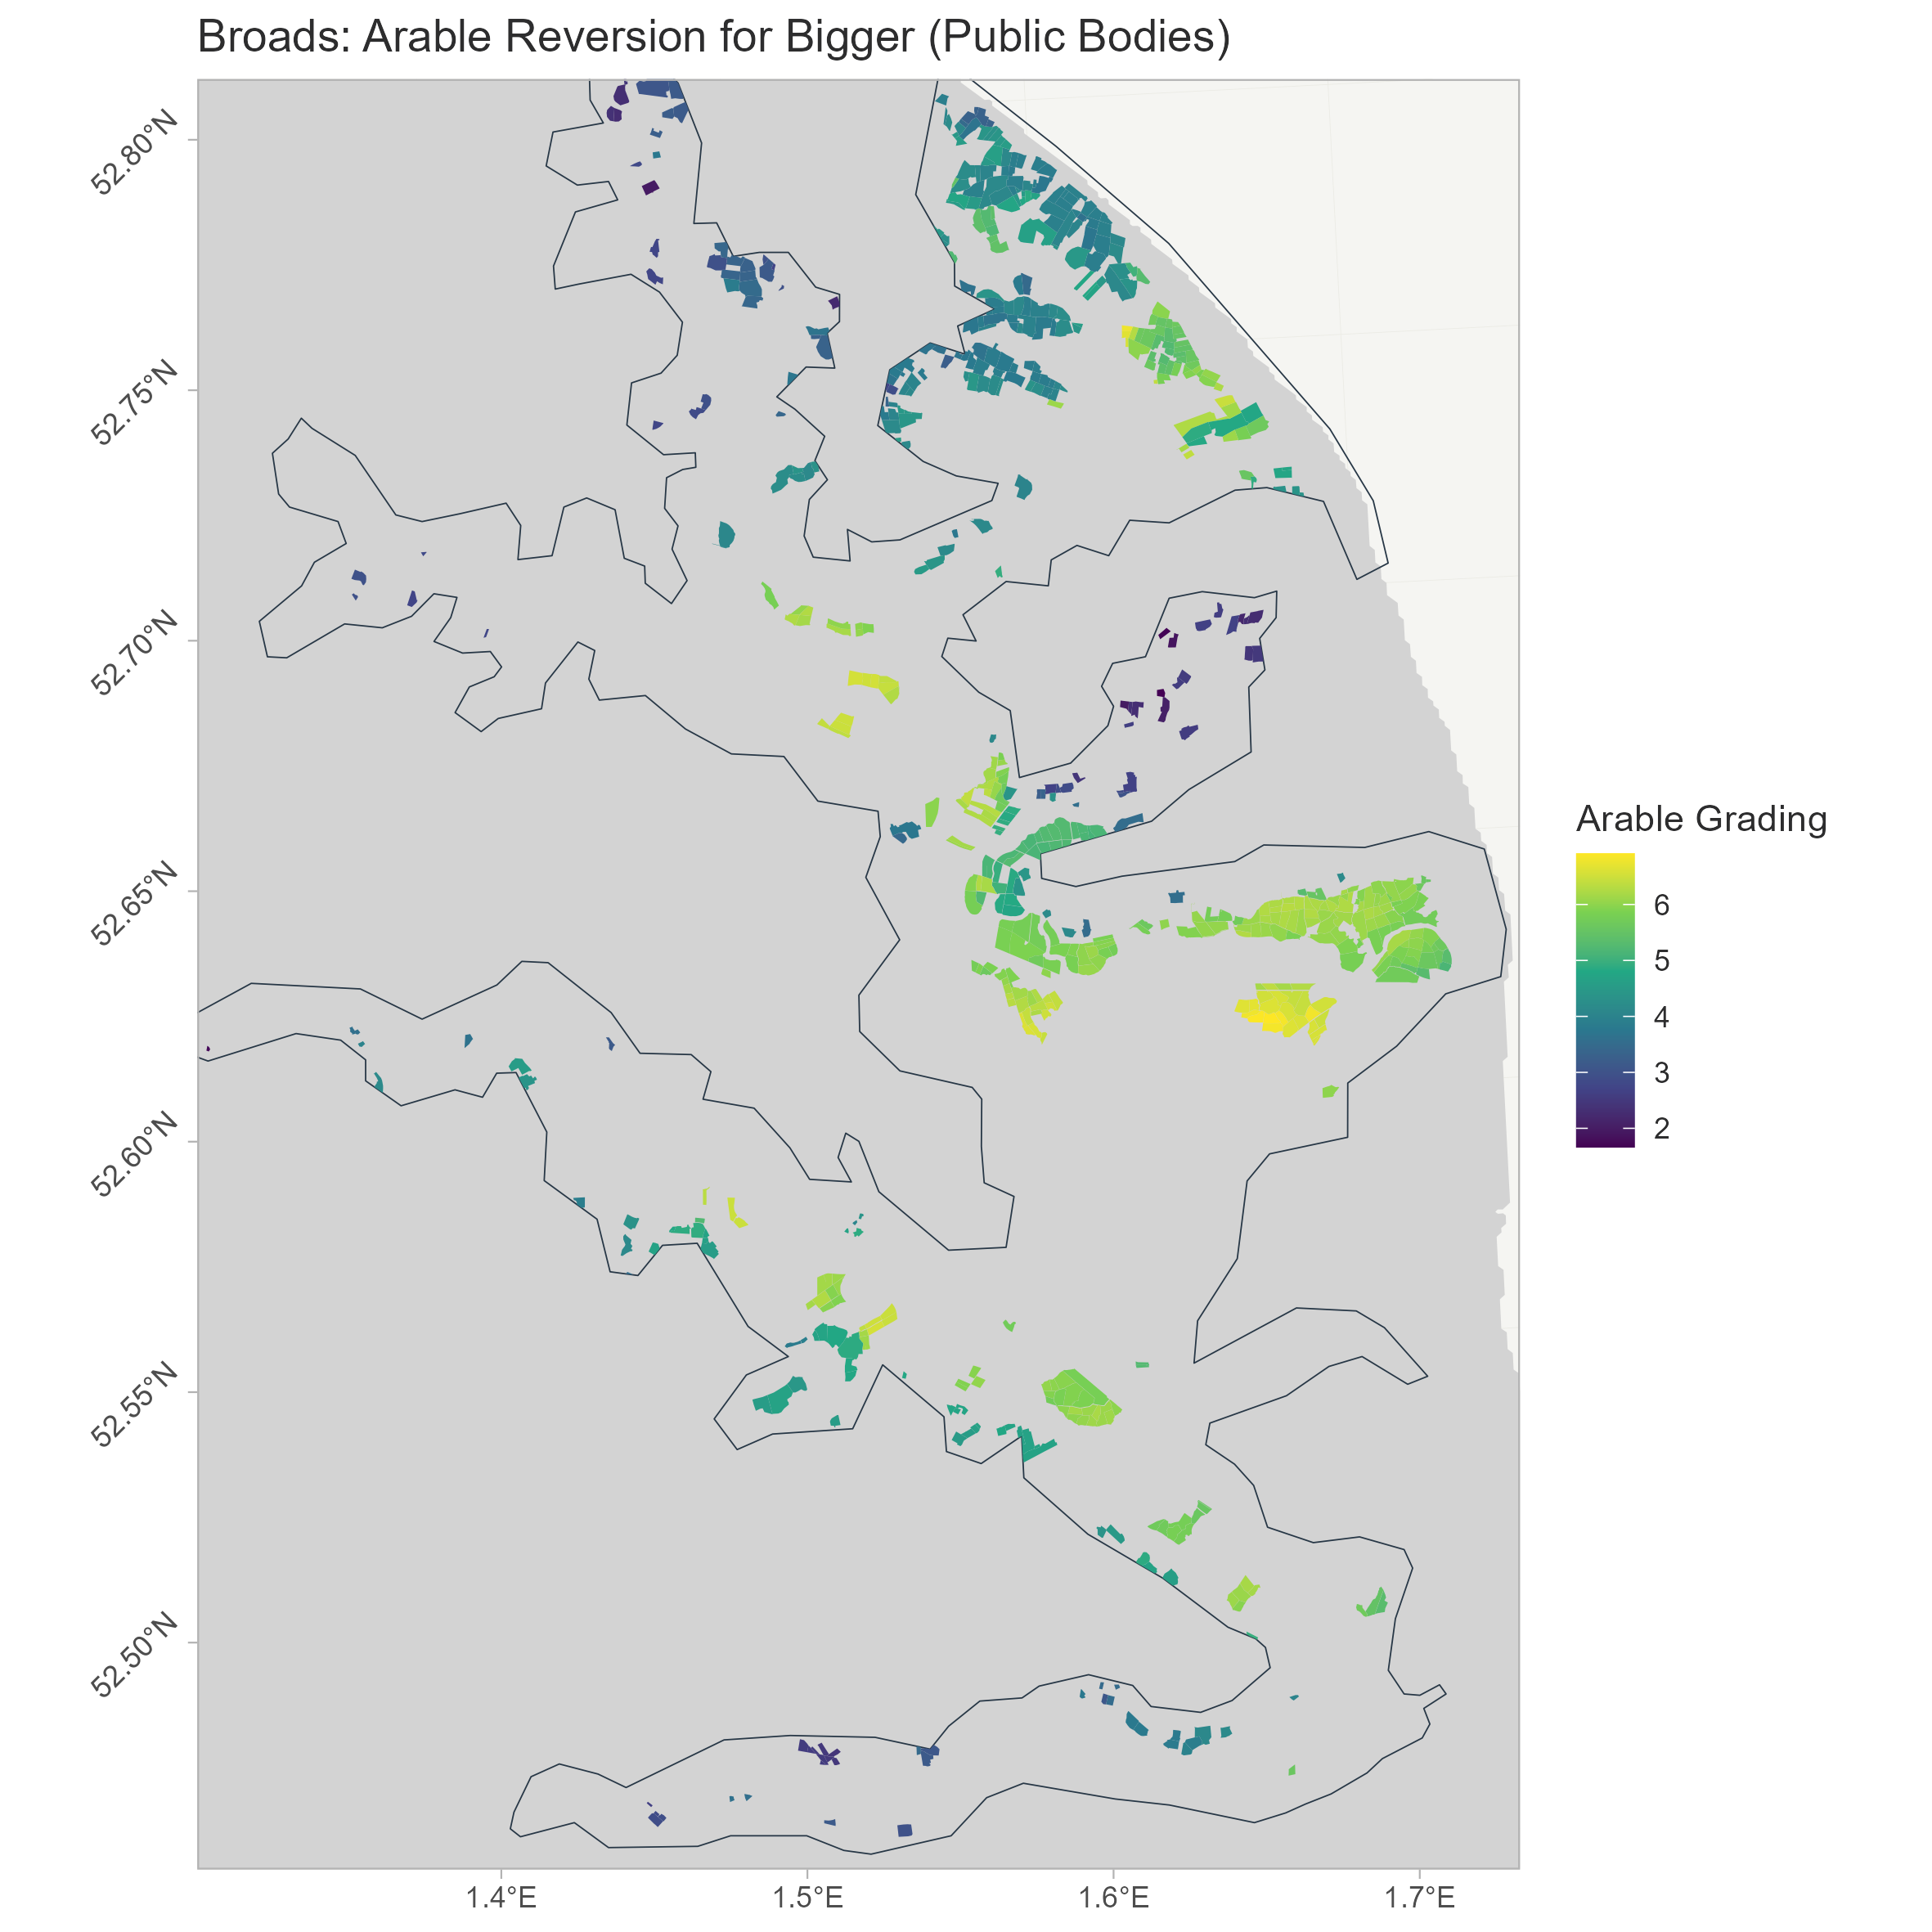
\includegraphics[width=\textwidth,height=9.375in]{Plots/Broads_G2_ArableBig.png}

}

\caption{\label{fig-BroadsArBigG2}Stakeholder gradings for group 2 in
the Norfolk Broads for the reversion of arable land to lowland wet
grassland under the bigger principle of nature restoration}

\end{figure}%

\newpage{}

\paragraph{Norfolk Broads: Arable Conversion for
More}\label{norfolk-broads-arable-conversion-for-more}

The stakeholder preferences for the conversion of arable land to lowland
wet grassland under the more principle of nature restoration for group 1
(Figure~\ref{fig-BroadsArMoreG1}) and 2
(Figure~\ref{fig-BroadsArMoreG2}).

\begin{figure}[H]

\centering{

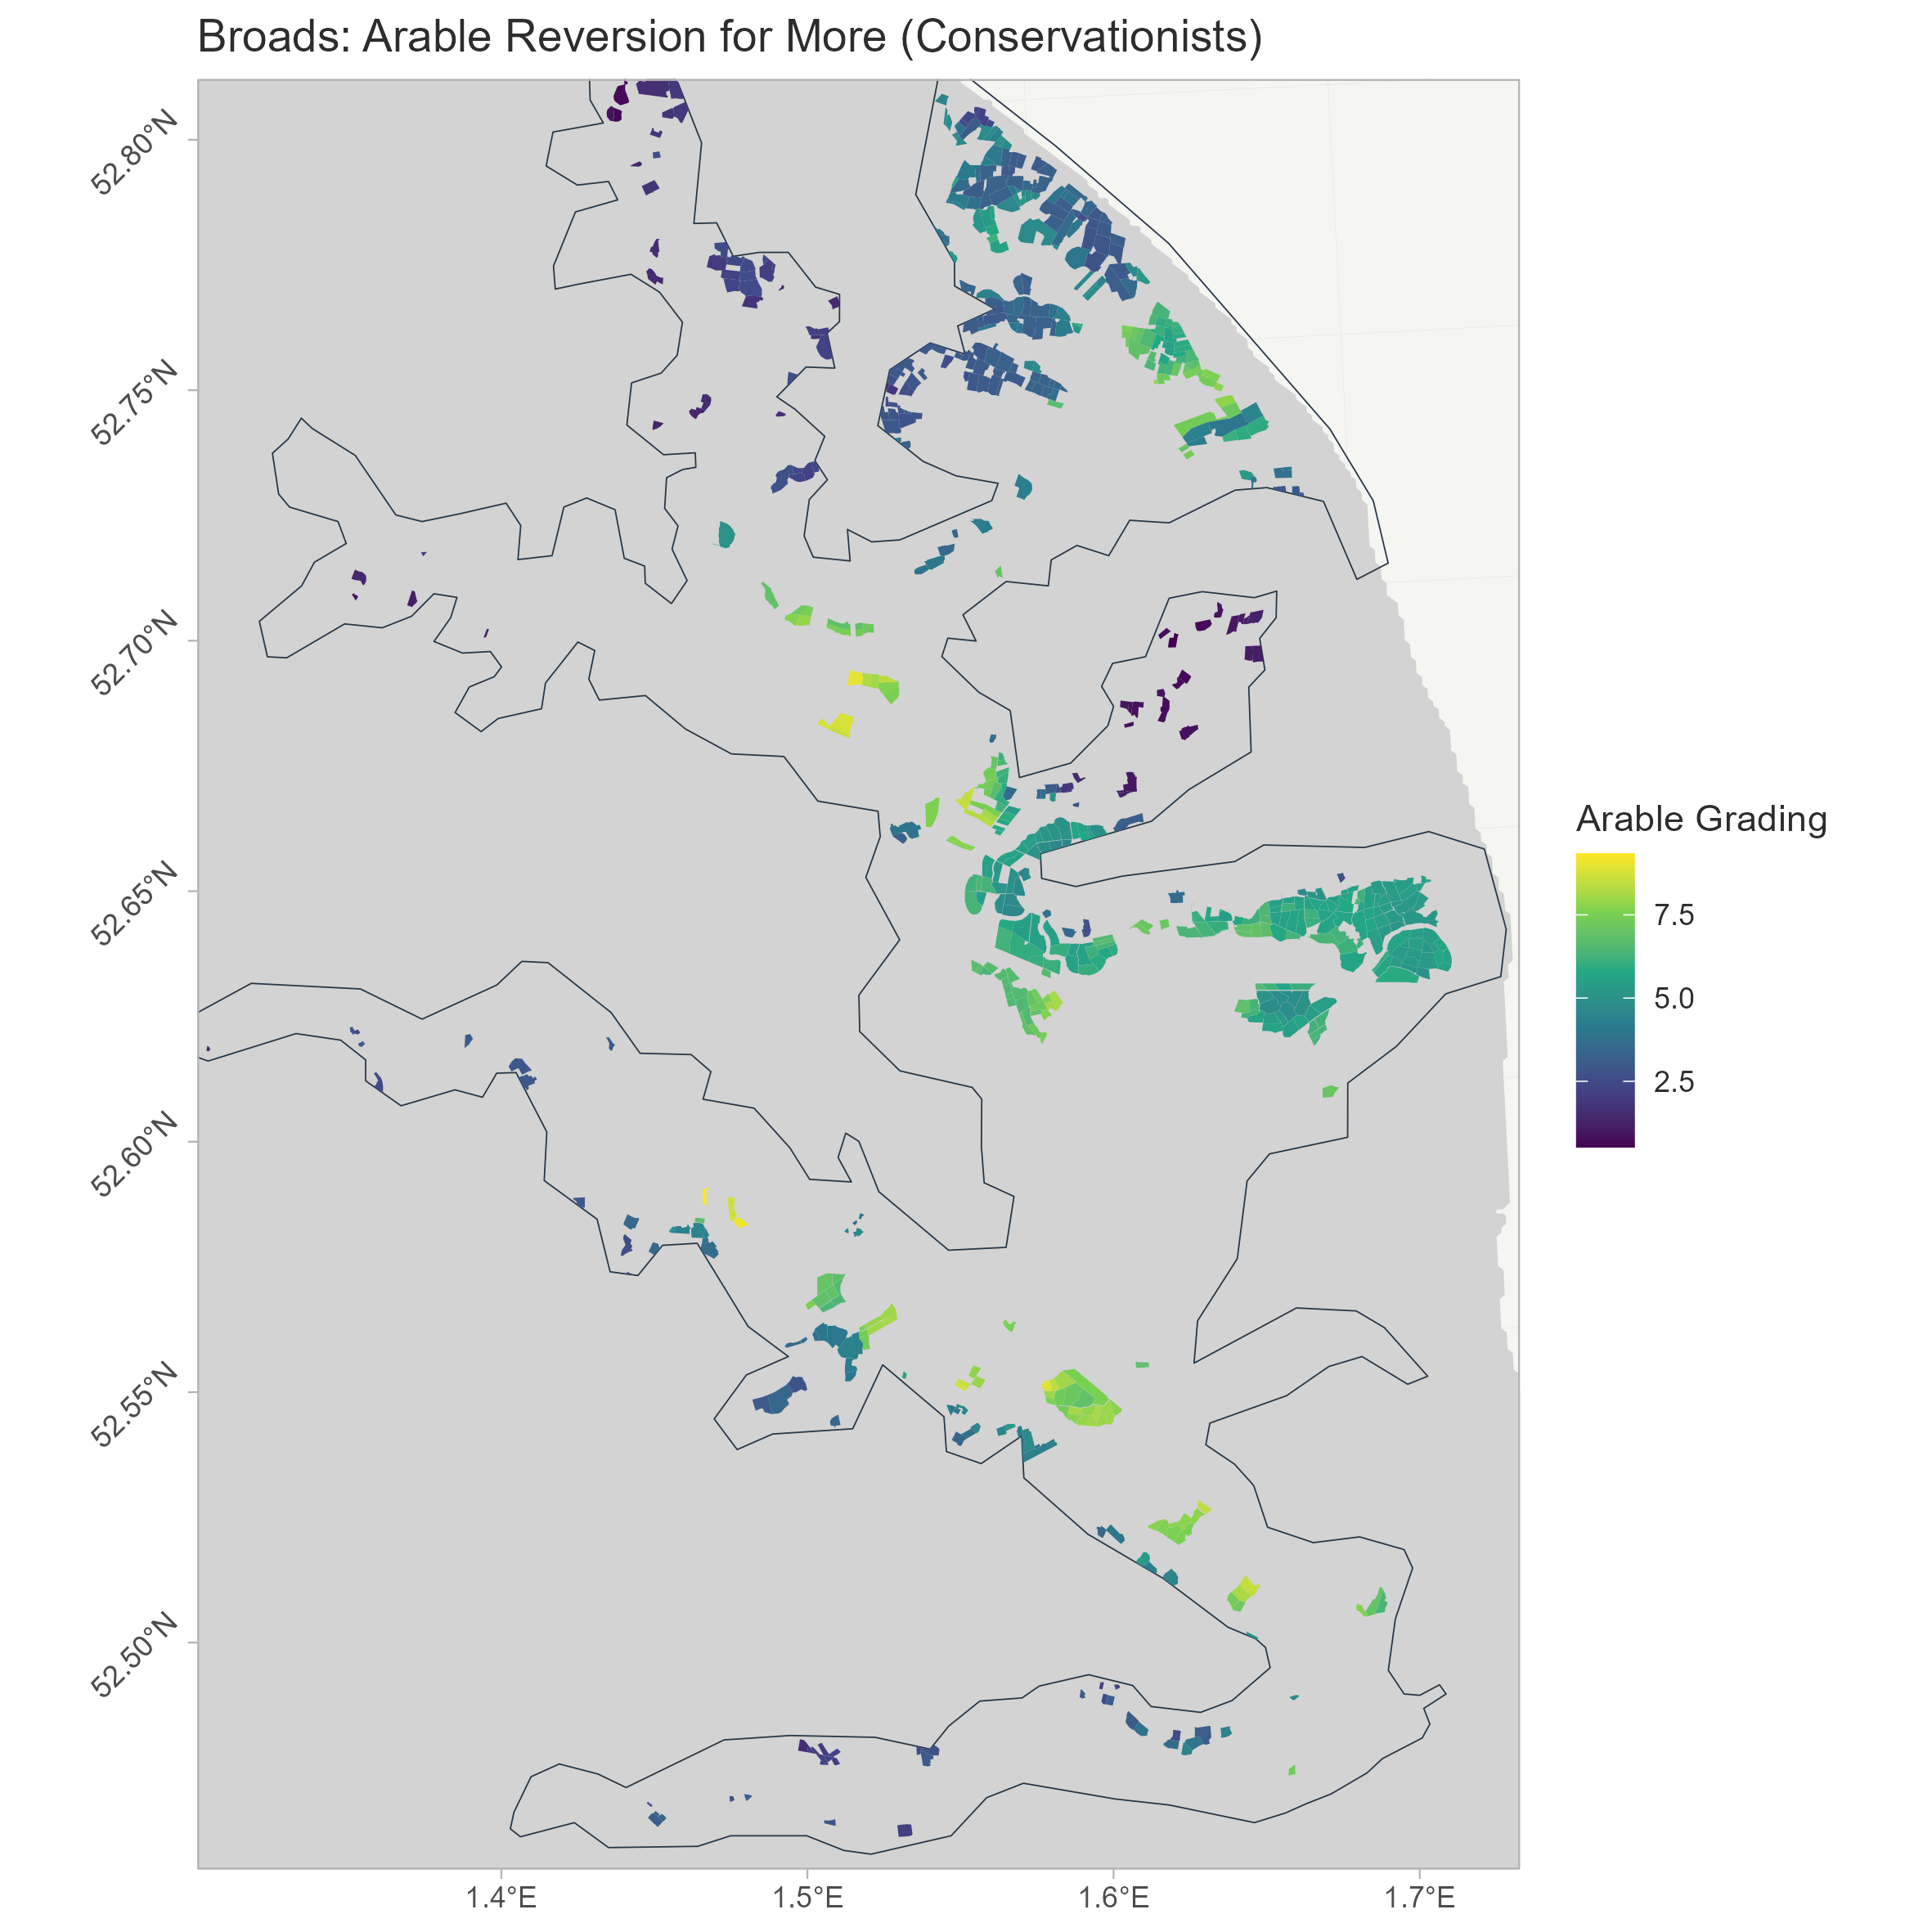
\includegraphics[width=\textwidth,height=9.375in]{Plots/Broads_G1_ArableMore.png}

}

\caption{\label{fig-BroadsArMoreG1}Stakeholder gradings for group 1 in
the Norfolk Broads for the reversion of arable land to lowland wet
grassland under the more principle of nature restoration}

\end{figure}%

\begin{figure}[H]

\centering{

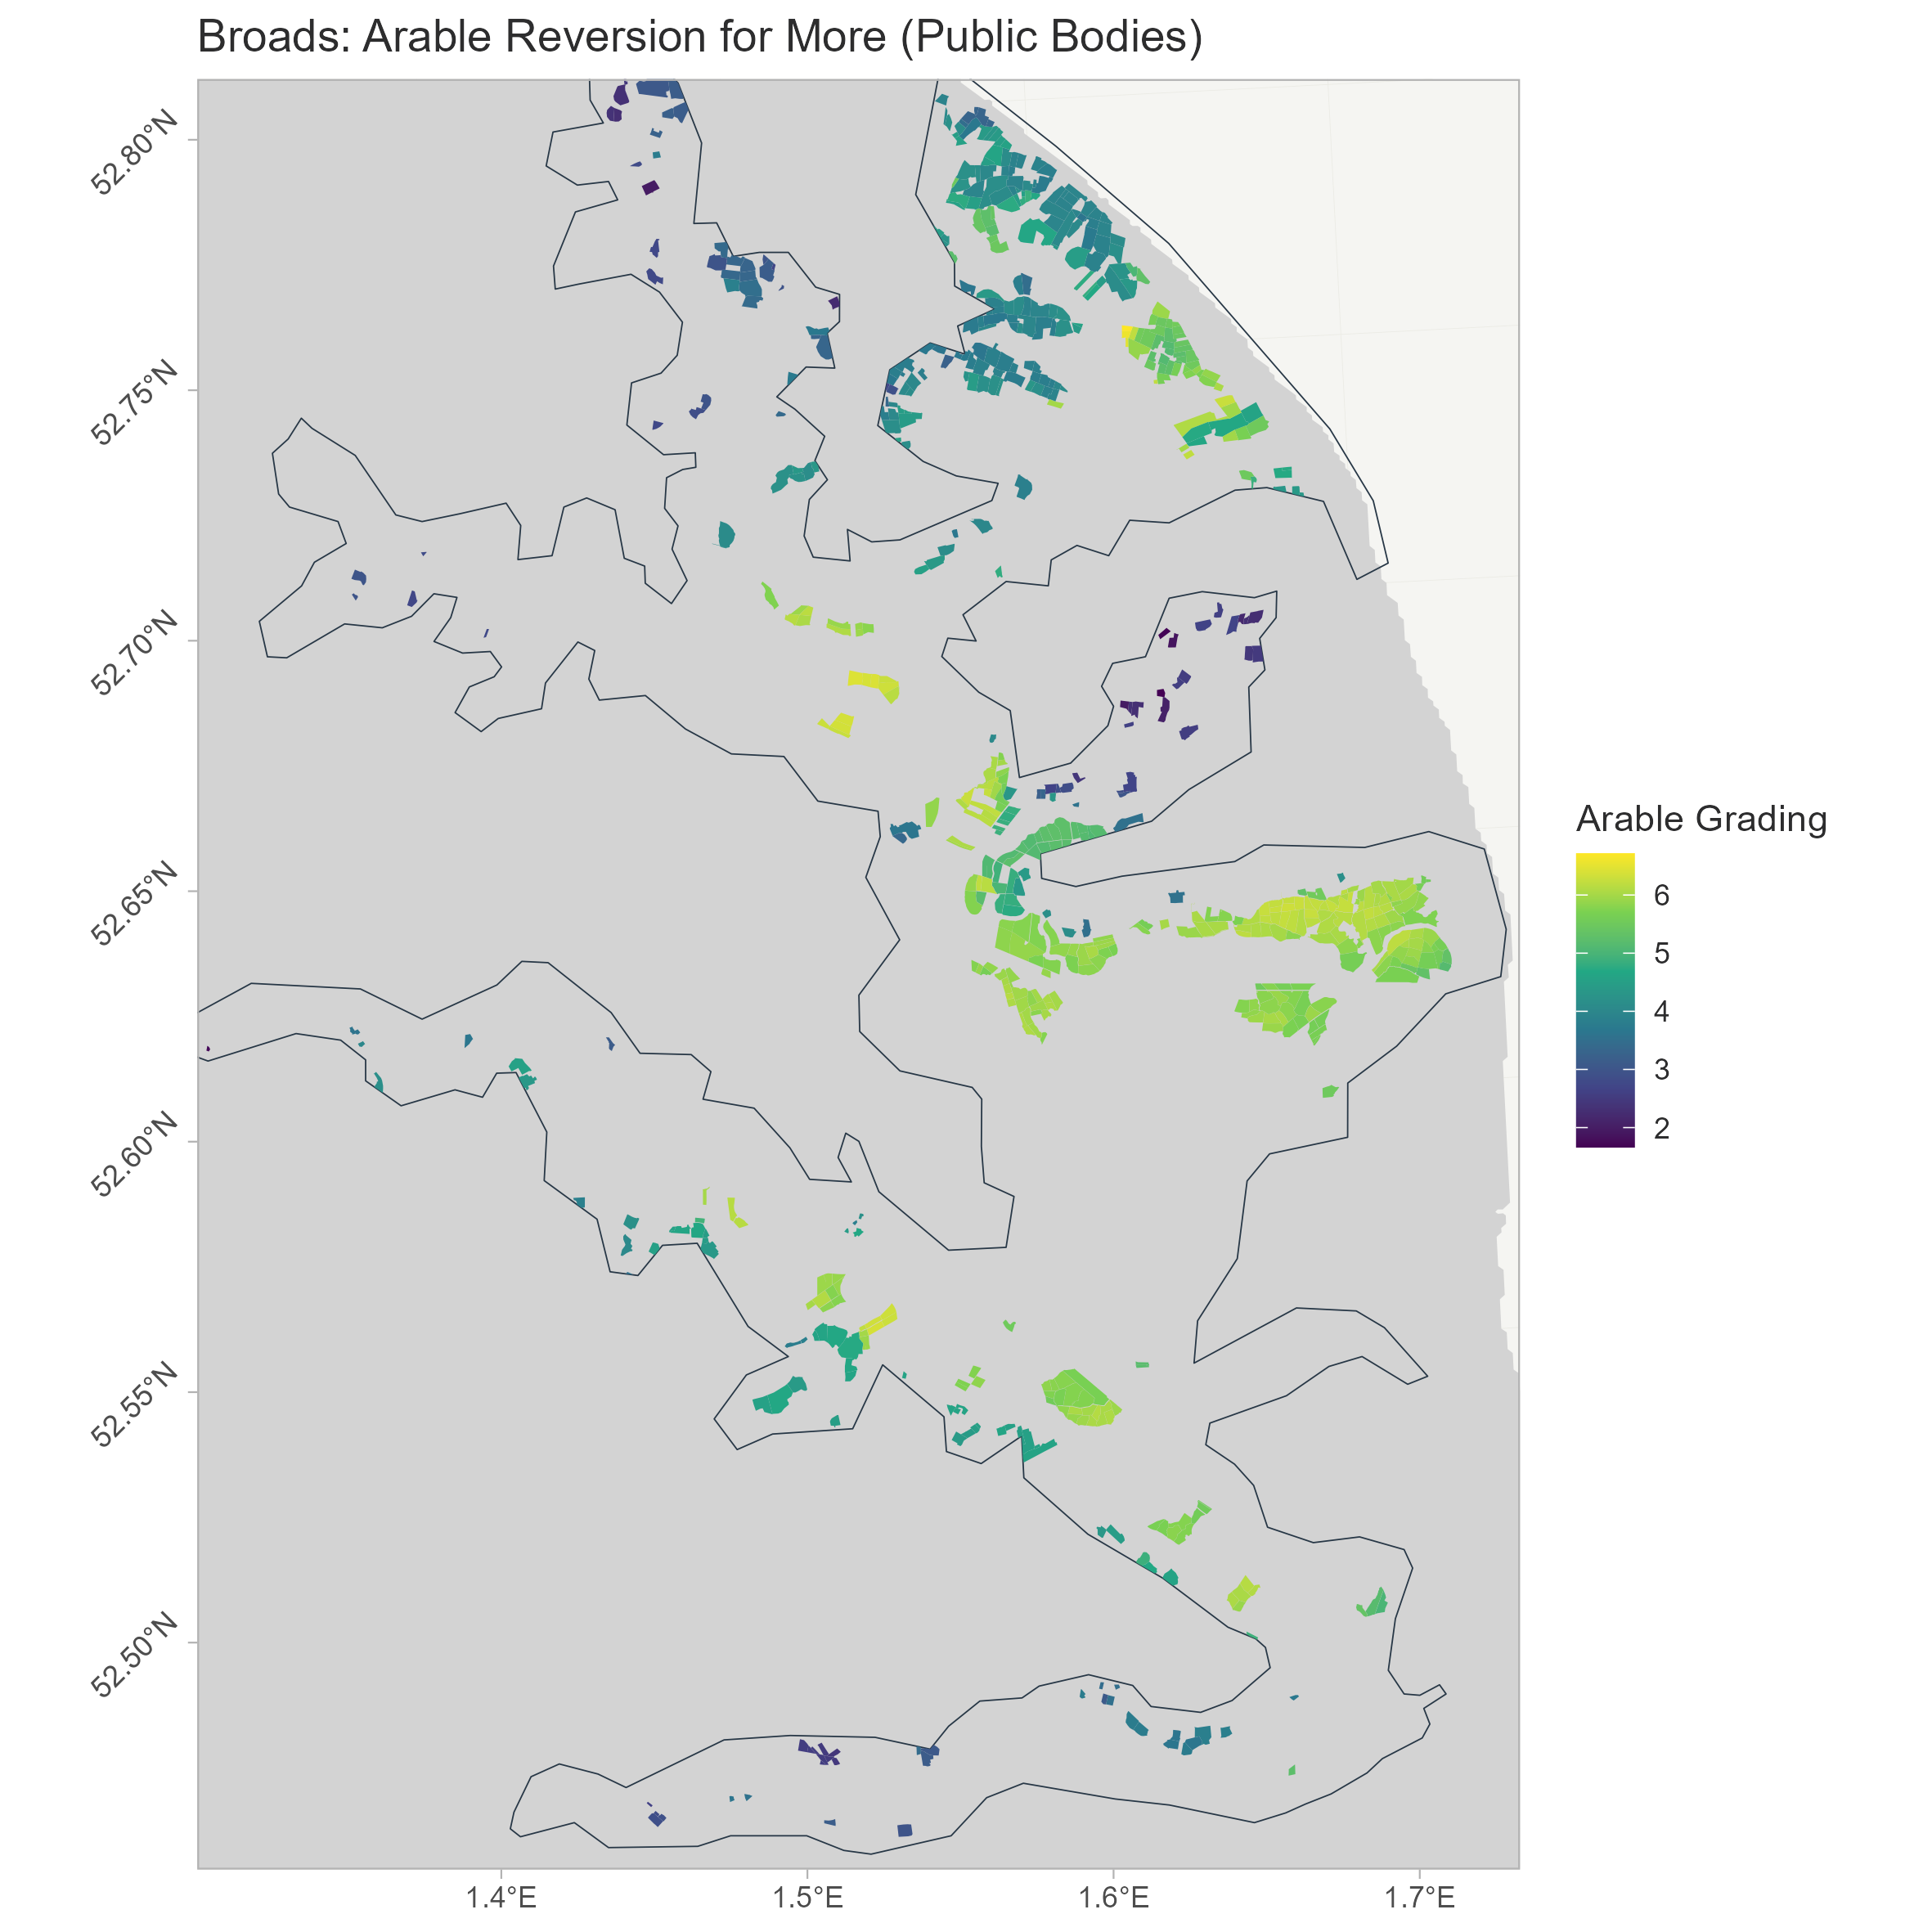
\includegraphics[width=\textwidth,height=9.375in]{Plots/Broads_G2_ArableMore.png}

}

\caption{\label{fig-BroadsArMoreG2}Stakeholder gradings for group 2 in
the Norfolk Broads for the reversion of arable land to lowland wet
grassland under the more principle of nature restoration}

\end{figure}%

\newpage{}

\subsubsection{North Kent Results}\label{north-kent-results}

For North Kent we had two different stakeholder groups. Group 1 (G1) was
a group of conservationists and group 2 was a group of landowners and
farmers.

\paragraph{North Kent: Better}\label{north-kent-better}

The stakeholder preferences for the better principle of nature
restoration for group 1 and group 2 can be visualized in
(Figure~\ref{fig-NKBetterG1}) and (Figure~\ref{fig-NKBetterG2}),
receptively. The stakeholder guidelines that were used to produce these
maps can be found in Table~\ref{tbl-KeG1} for group 1 and
Table~\ref{tbl-KeG2} for group 2.

\begin{figure}[H]

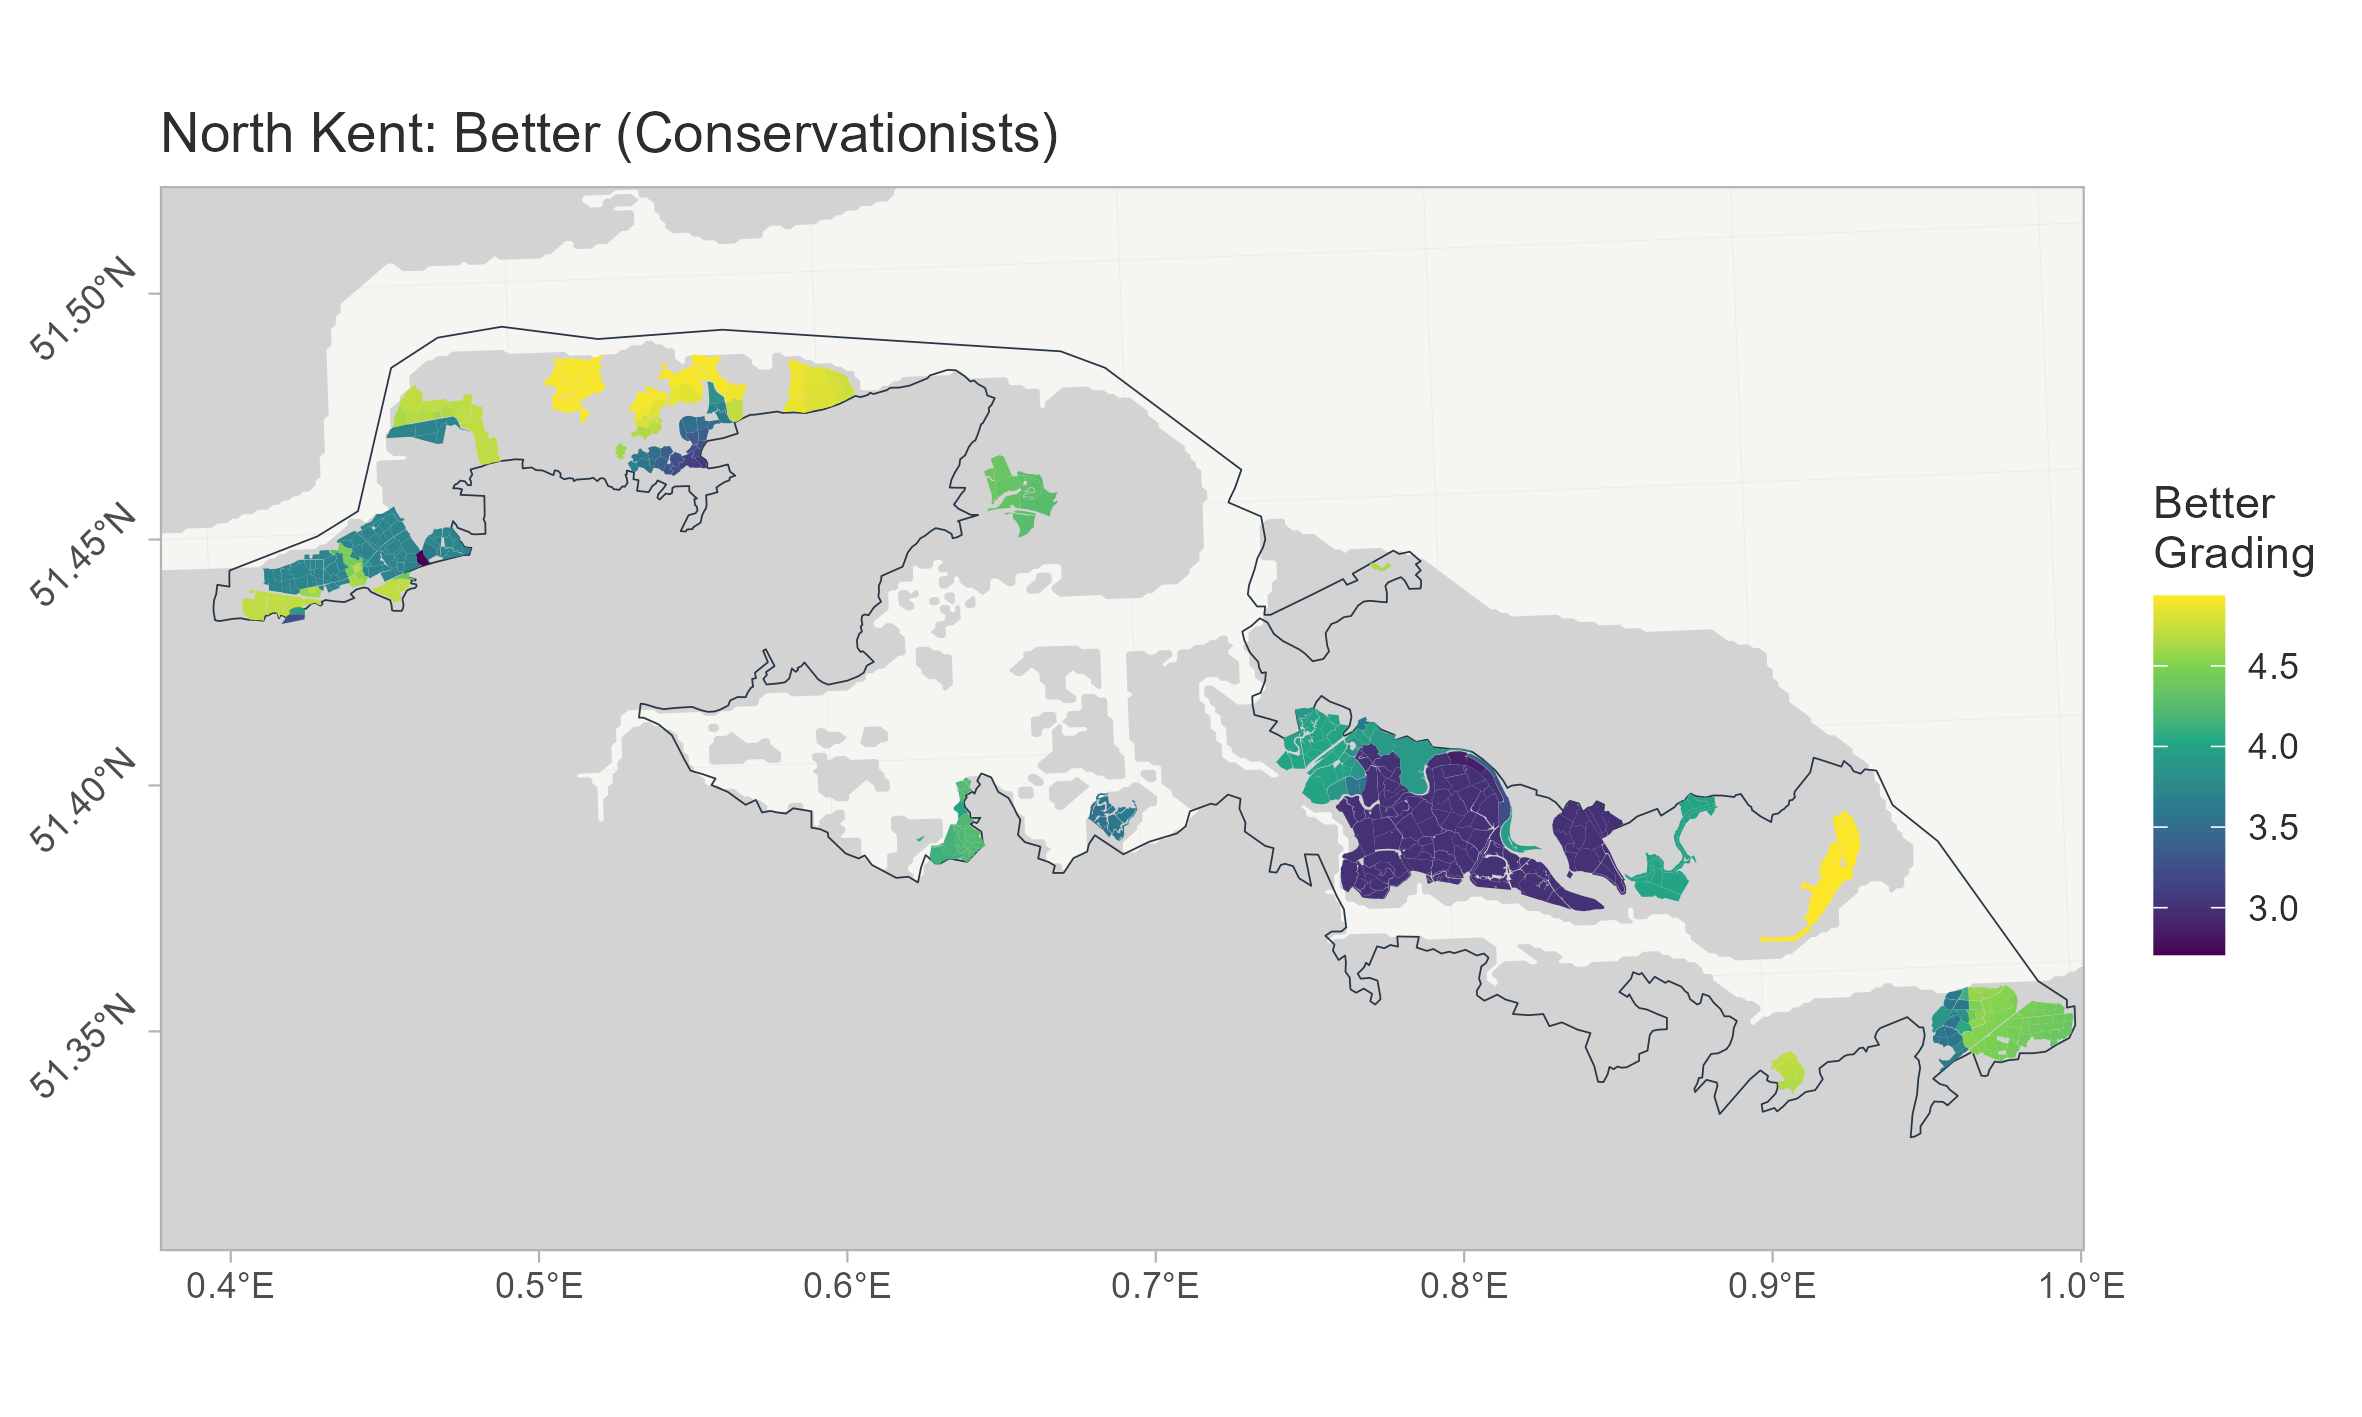
\includegraphics[width=7.29167in,height=\textheight]{Plots/NorthKent_G1_Better.png}

\caption{\label{fig-NKBetterG1}Stakeholder gradings for group 1 in North
Kent for the better principle of nature restoration}

\end{figure}%

\begin{figure}[H]

\centering{

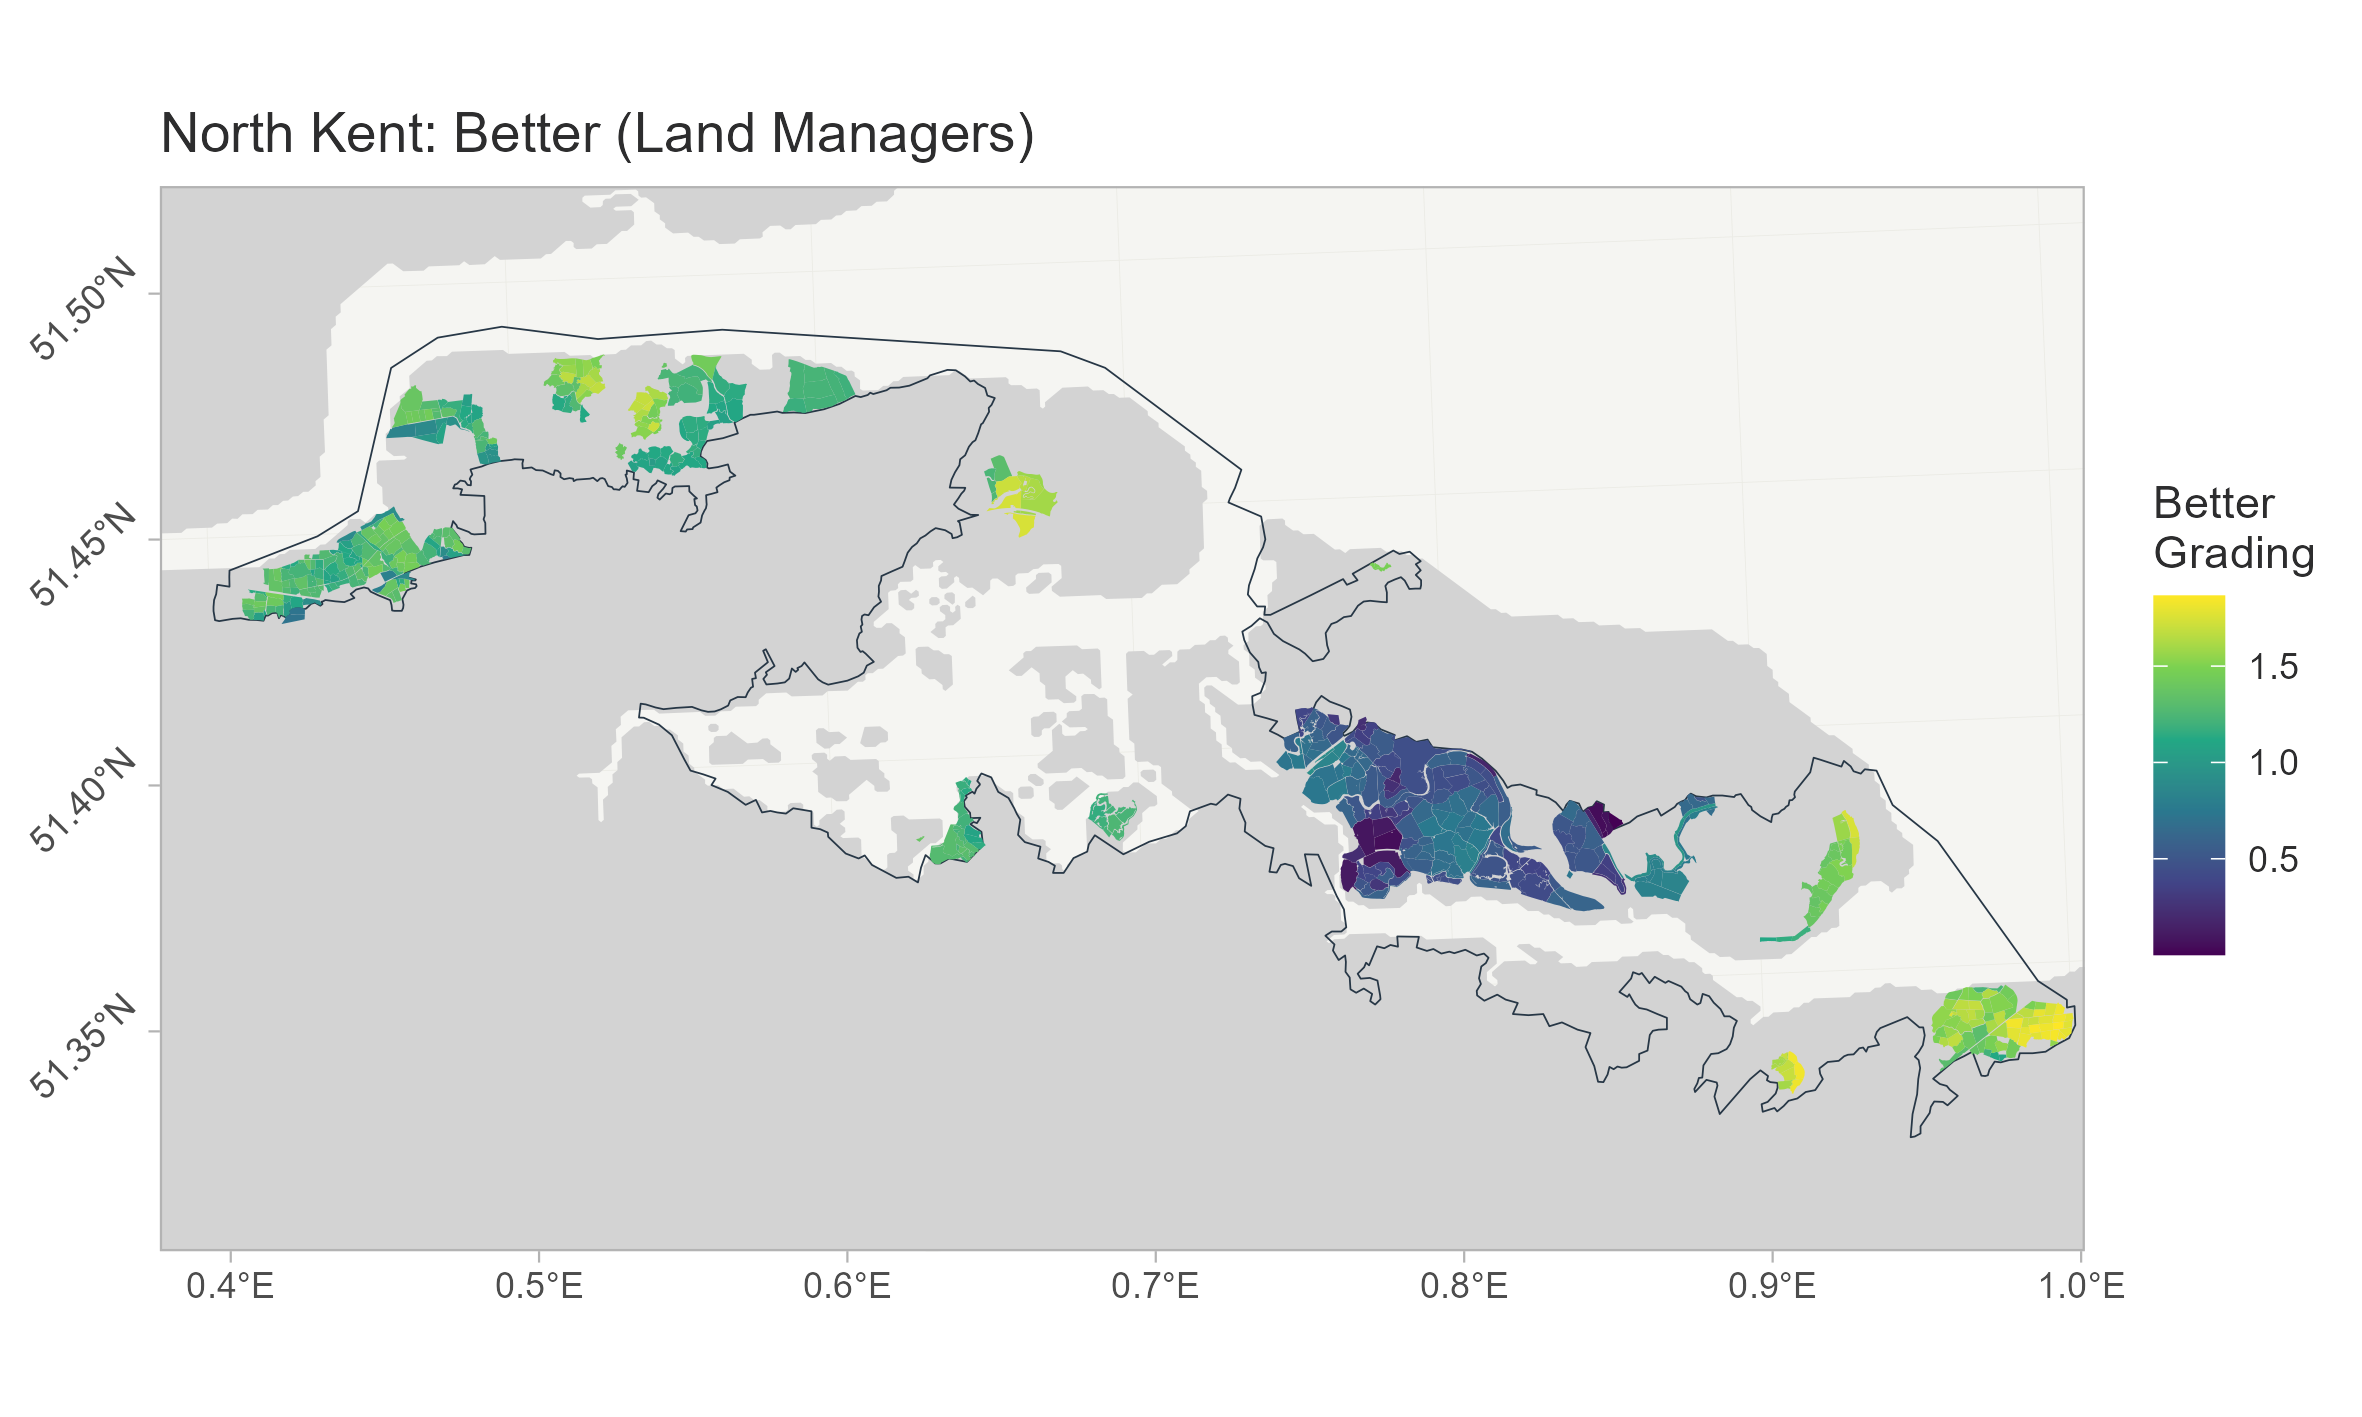
\includegraphics[width=7.29167in,height=\textheight]{Plots/NorthKent_G2_Better.png}

}

\caption{\label{fig-NKBetterG2}Stakeholder gradings for group 2 in North
Kent for the better principle of nature restoration}

\end{figure}%

\newpage{}

\paragraph{North Kent: Bigger}\label{north-kent-bigger}

The stakeholder preferences for the bigger principle of nature
restoration for group 1 (Figure~\ref{fig-NKBigG1}) and 2
(Figure~\ref{fig-NKBigG2}).

\begin{figure}[H]

\centering{

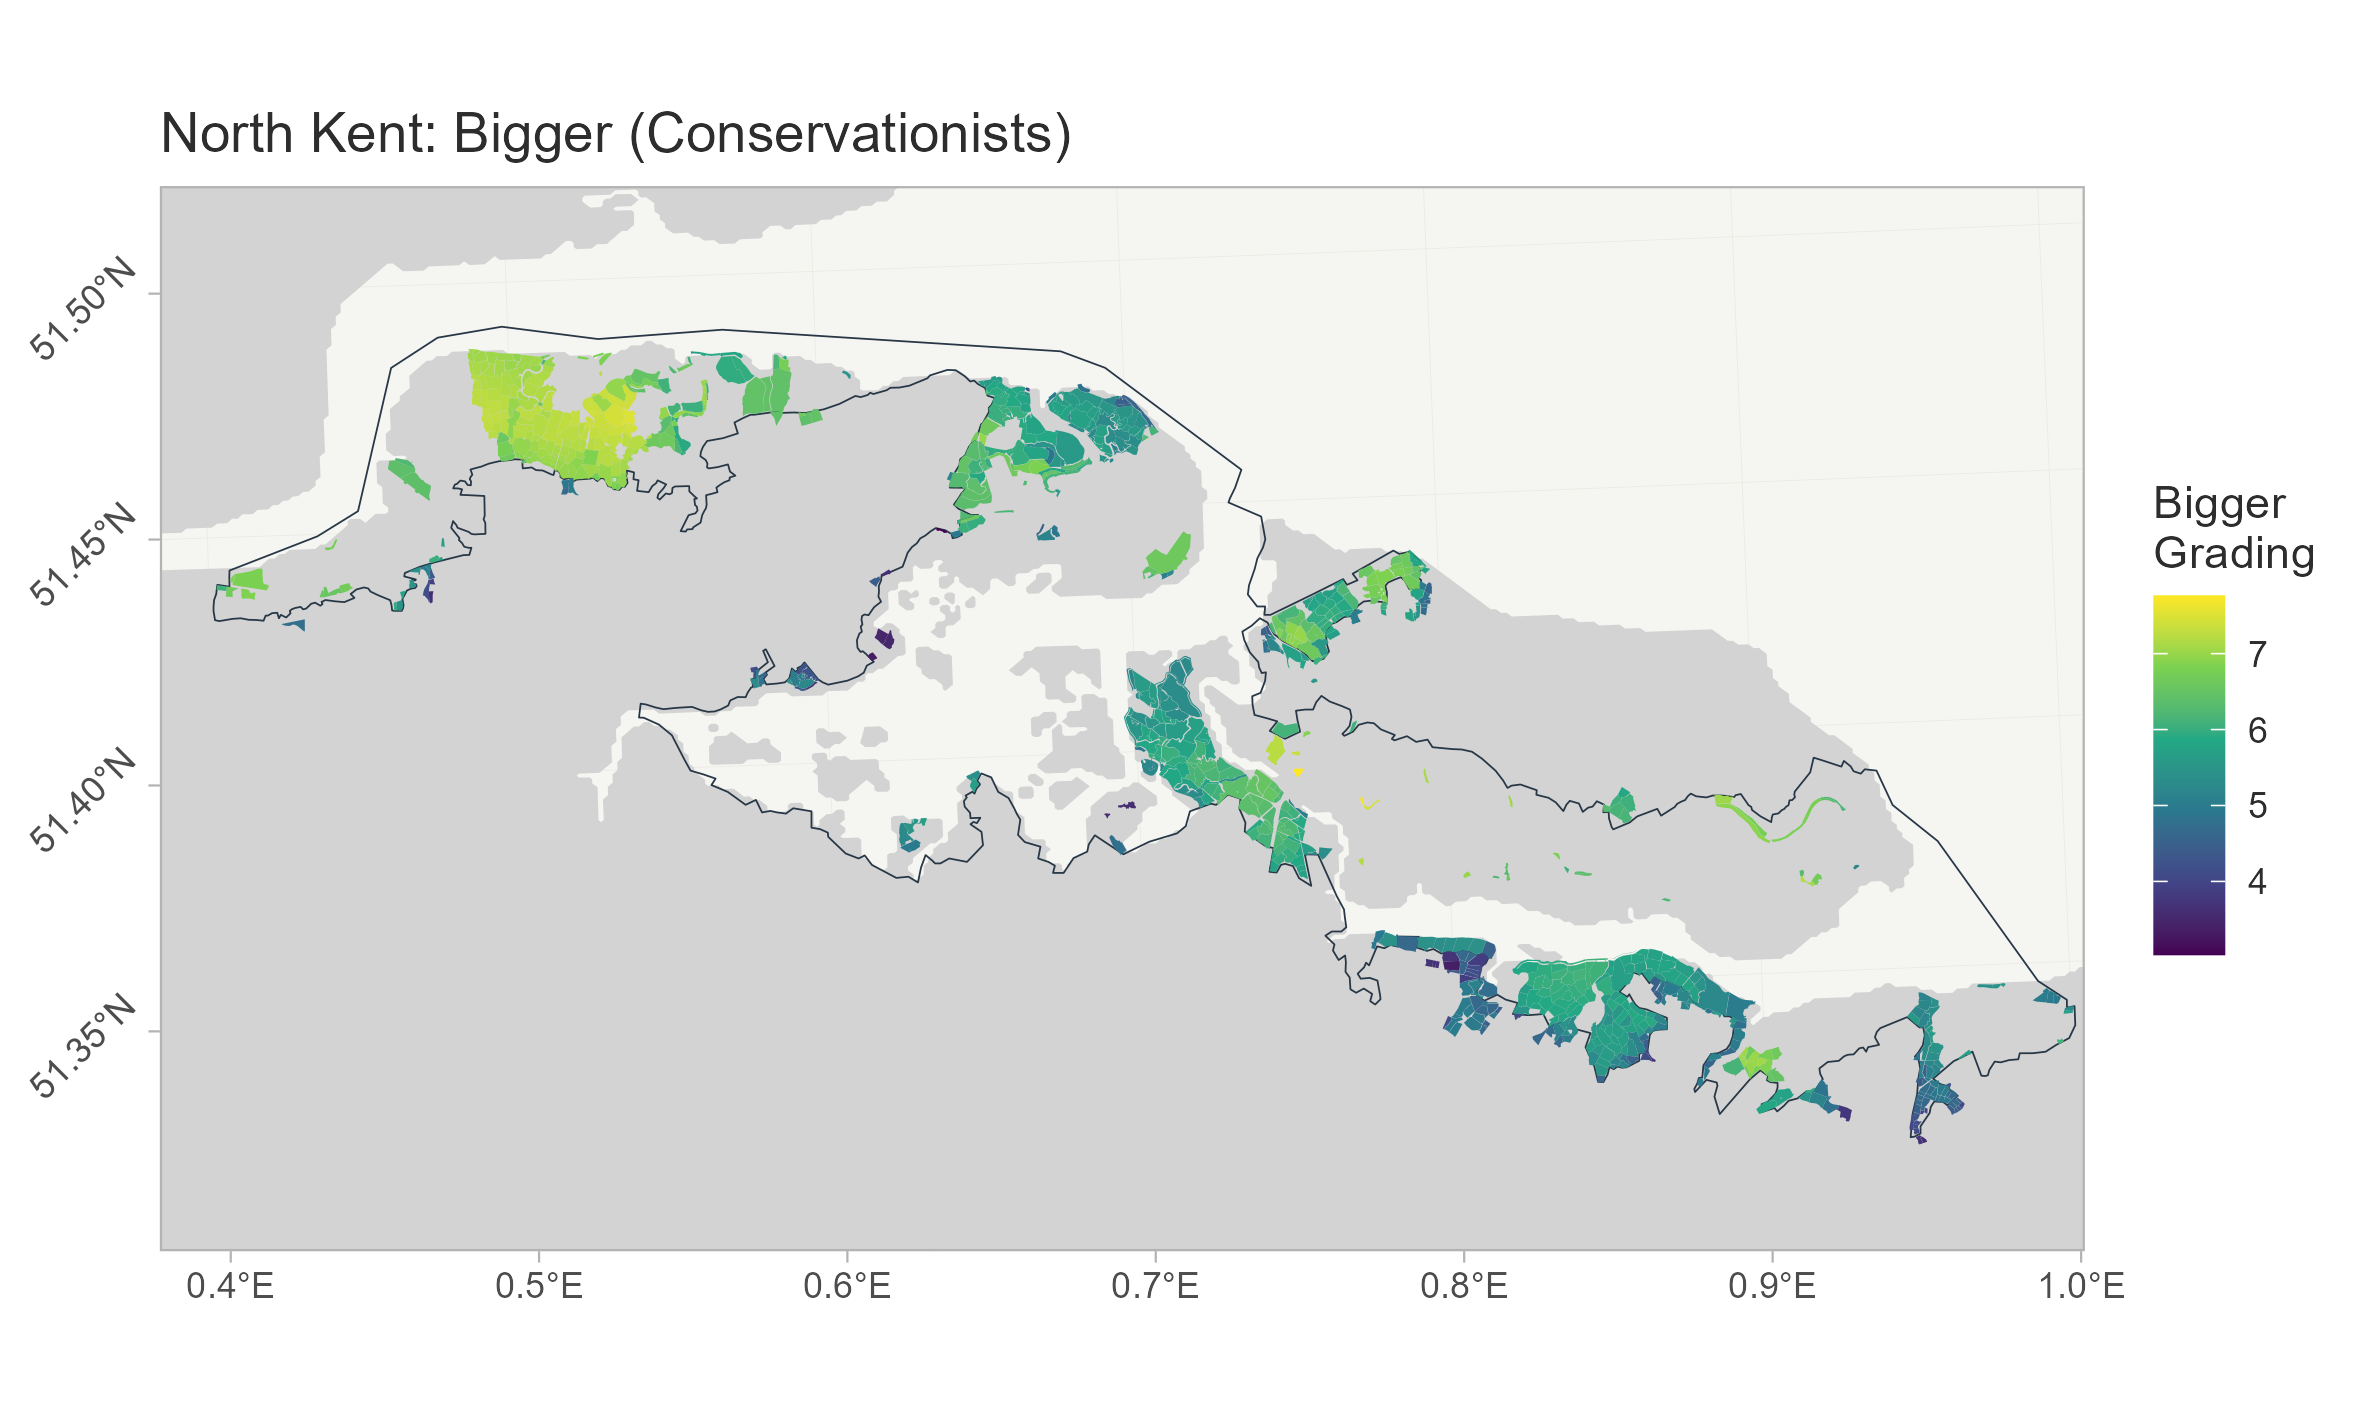
\includegraphics[width=7.29167in,height=\textheight]{Plots/NorthKent_G1_Bigger.png}

}

\caption{\label{fig-NKBigG1}Stakeholder gradings for group 1 in North
Kent for the bigger principle of nature restoration}

\end{figure}%

\begin{figure}[H]

\centering{

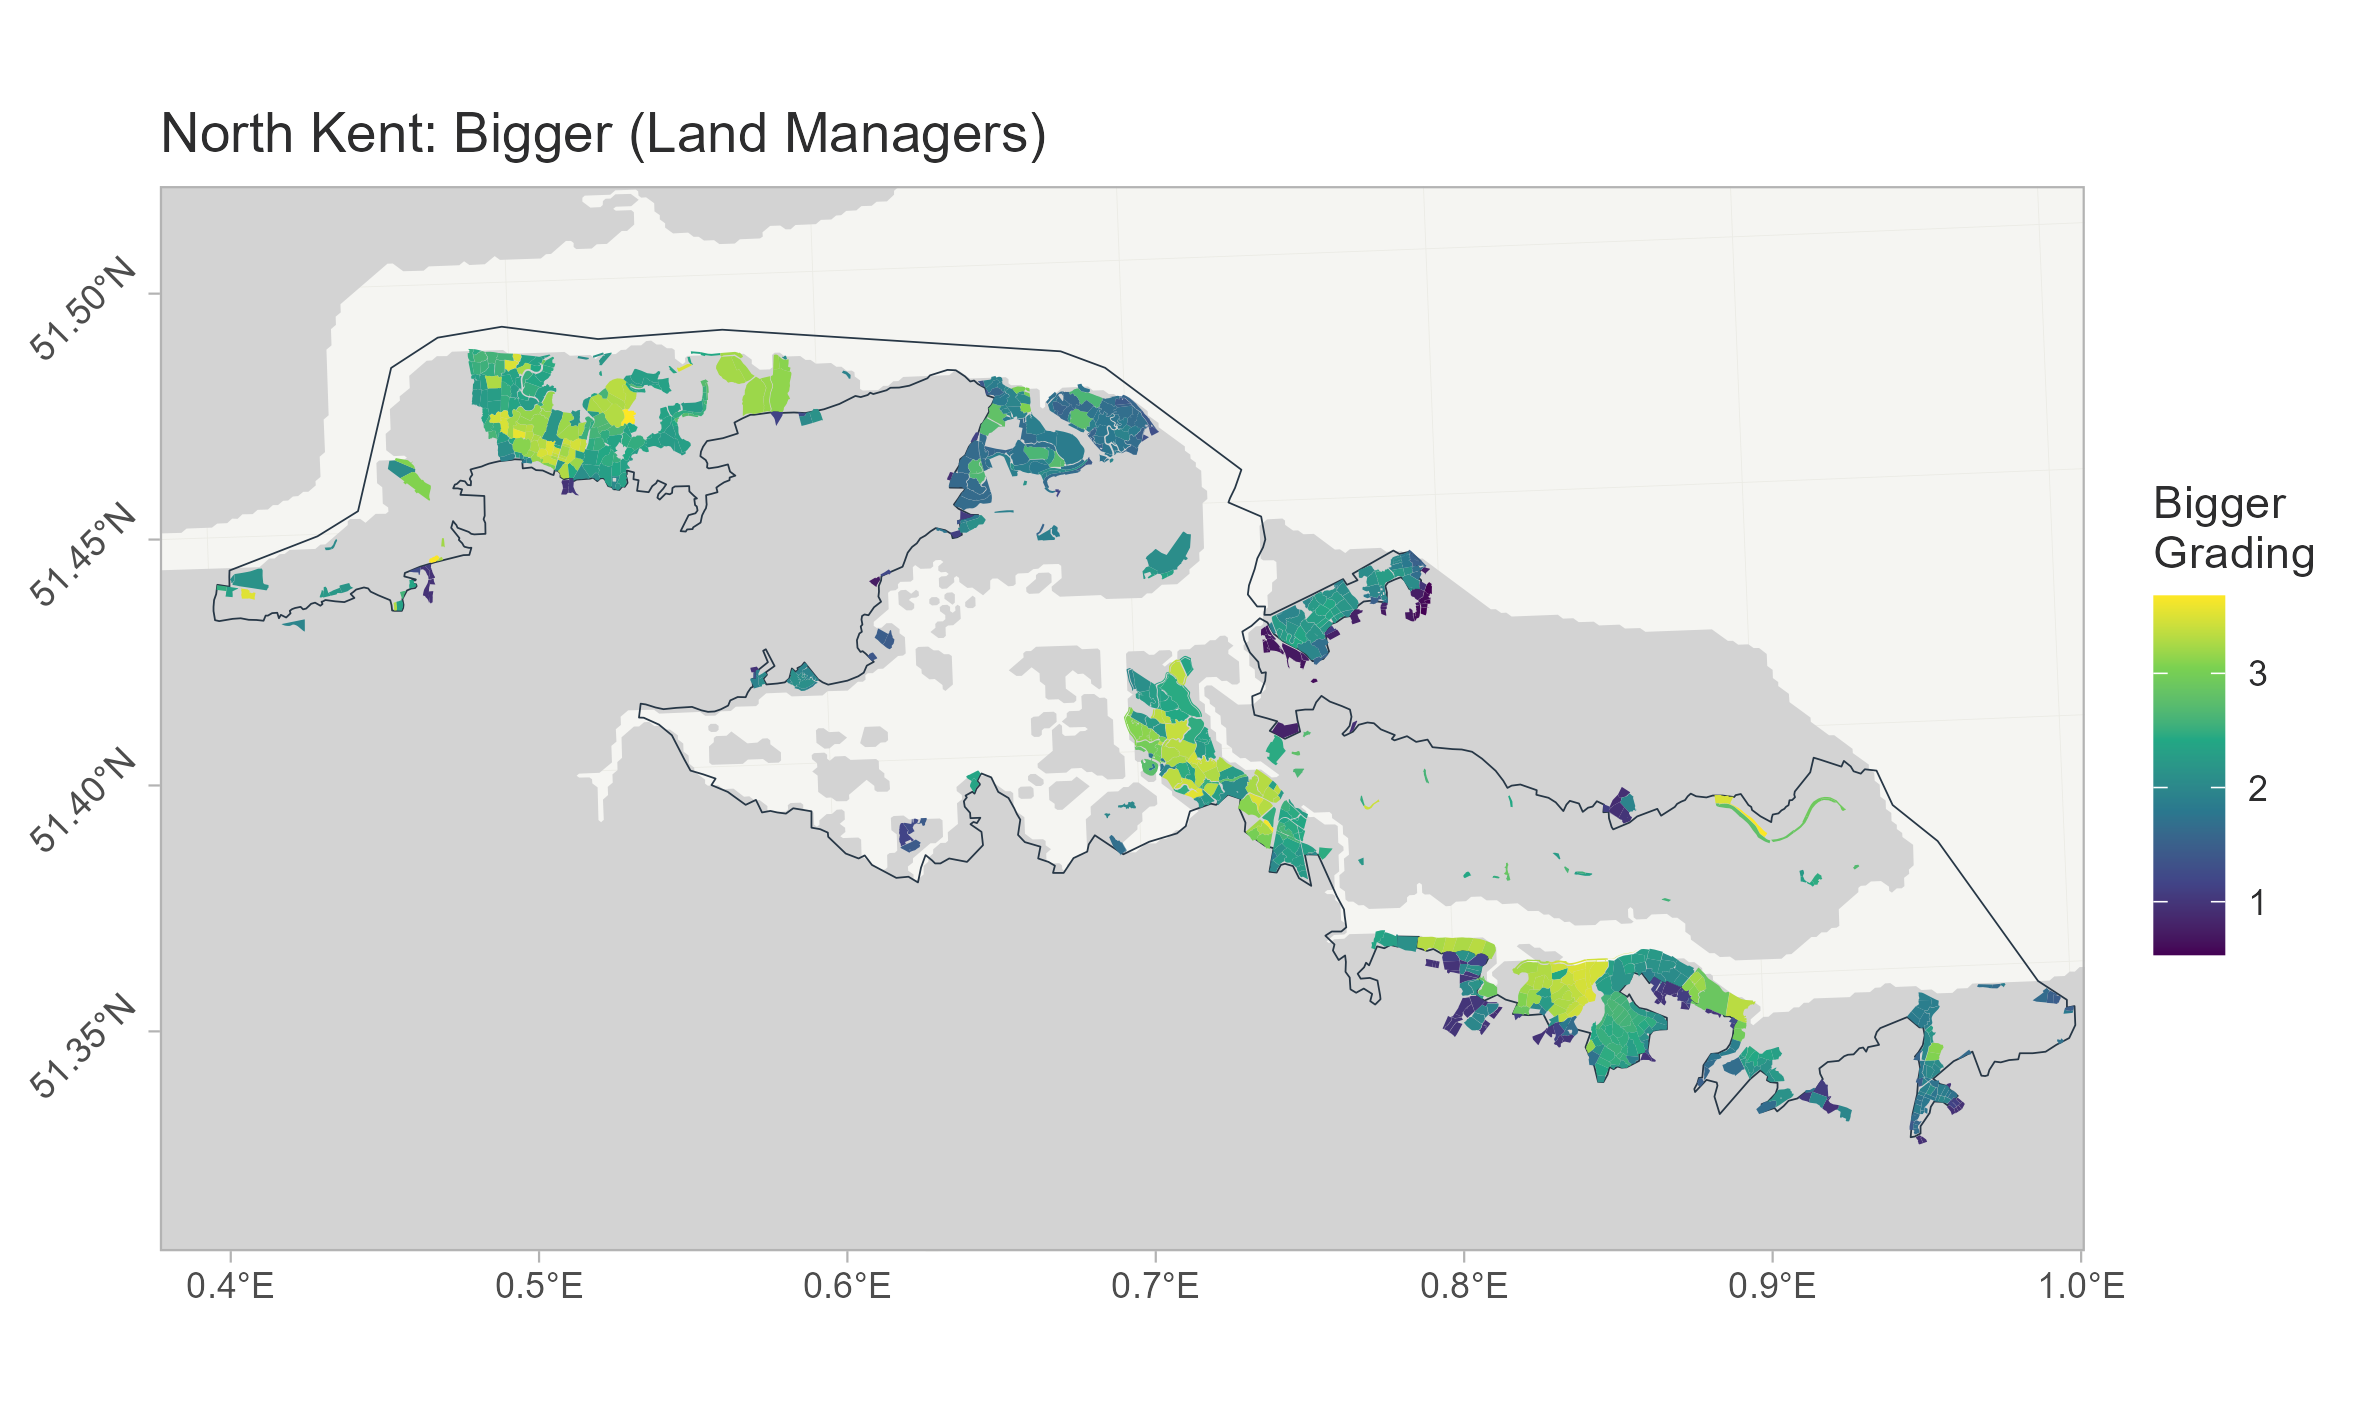
\includegraphics[width=7.29167in,height=\textheight]{Plots/NorthKent_G2_Bigger.png}

}

\caption{\label{fig-NKBigG2}Stakeholder gradings for group 2 in North
Kent for the bigger principle of nature restoration}

\end{figure}%

\newpage{}

\paragraph{North Kent: More}\label{north-kent-more}

The stakeholder preferences for the more principle of nature restoration
for group 1 (Figure~\ref{fig-NKMoreG1}) and 2
(Figure~\ref{fig-NKMoreG2}).

\begin{figure}[H]

\centering{

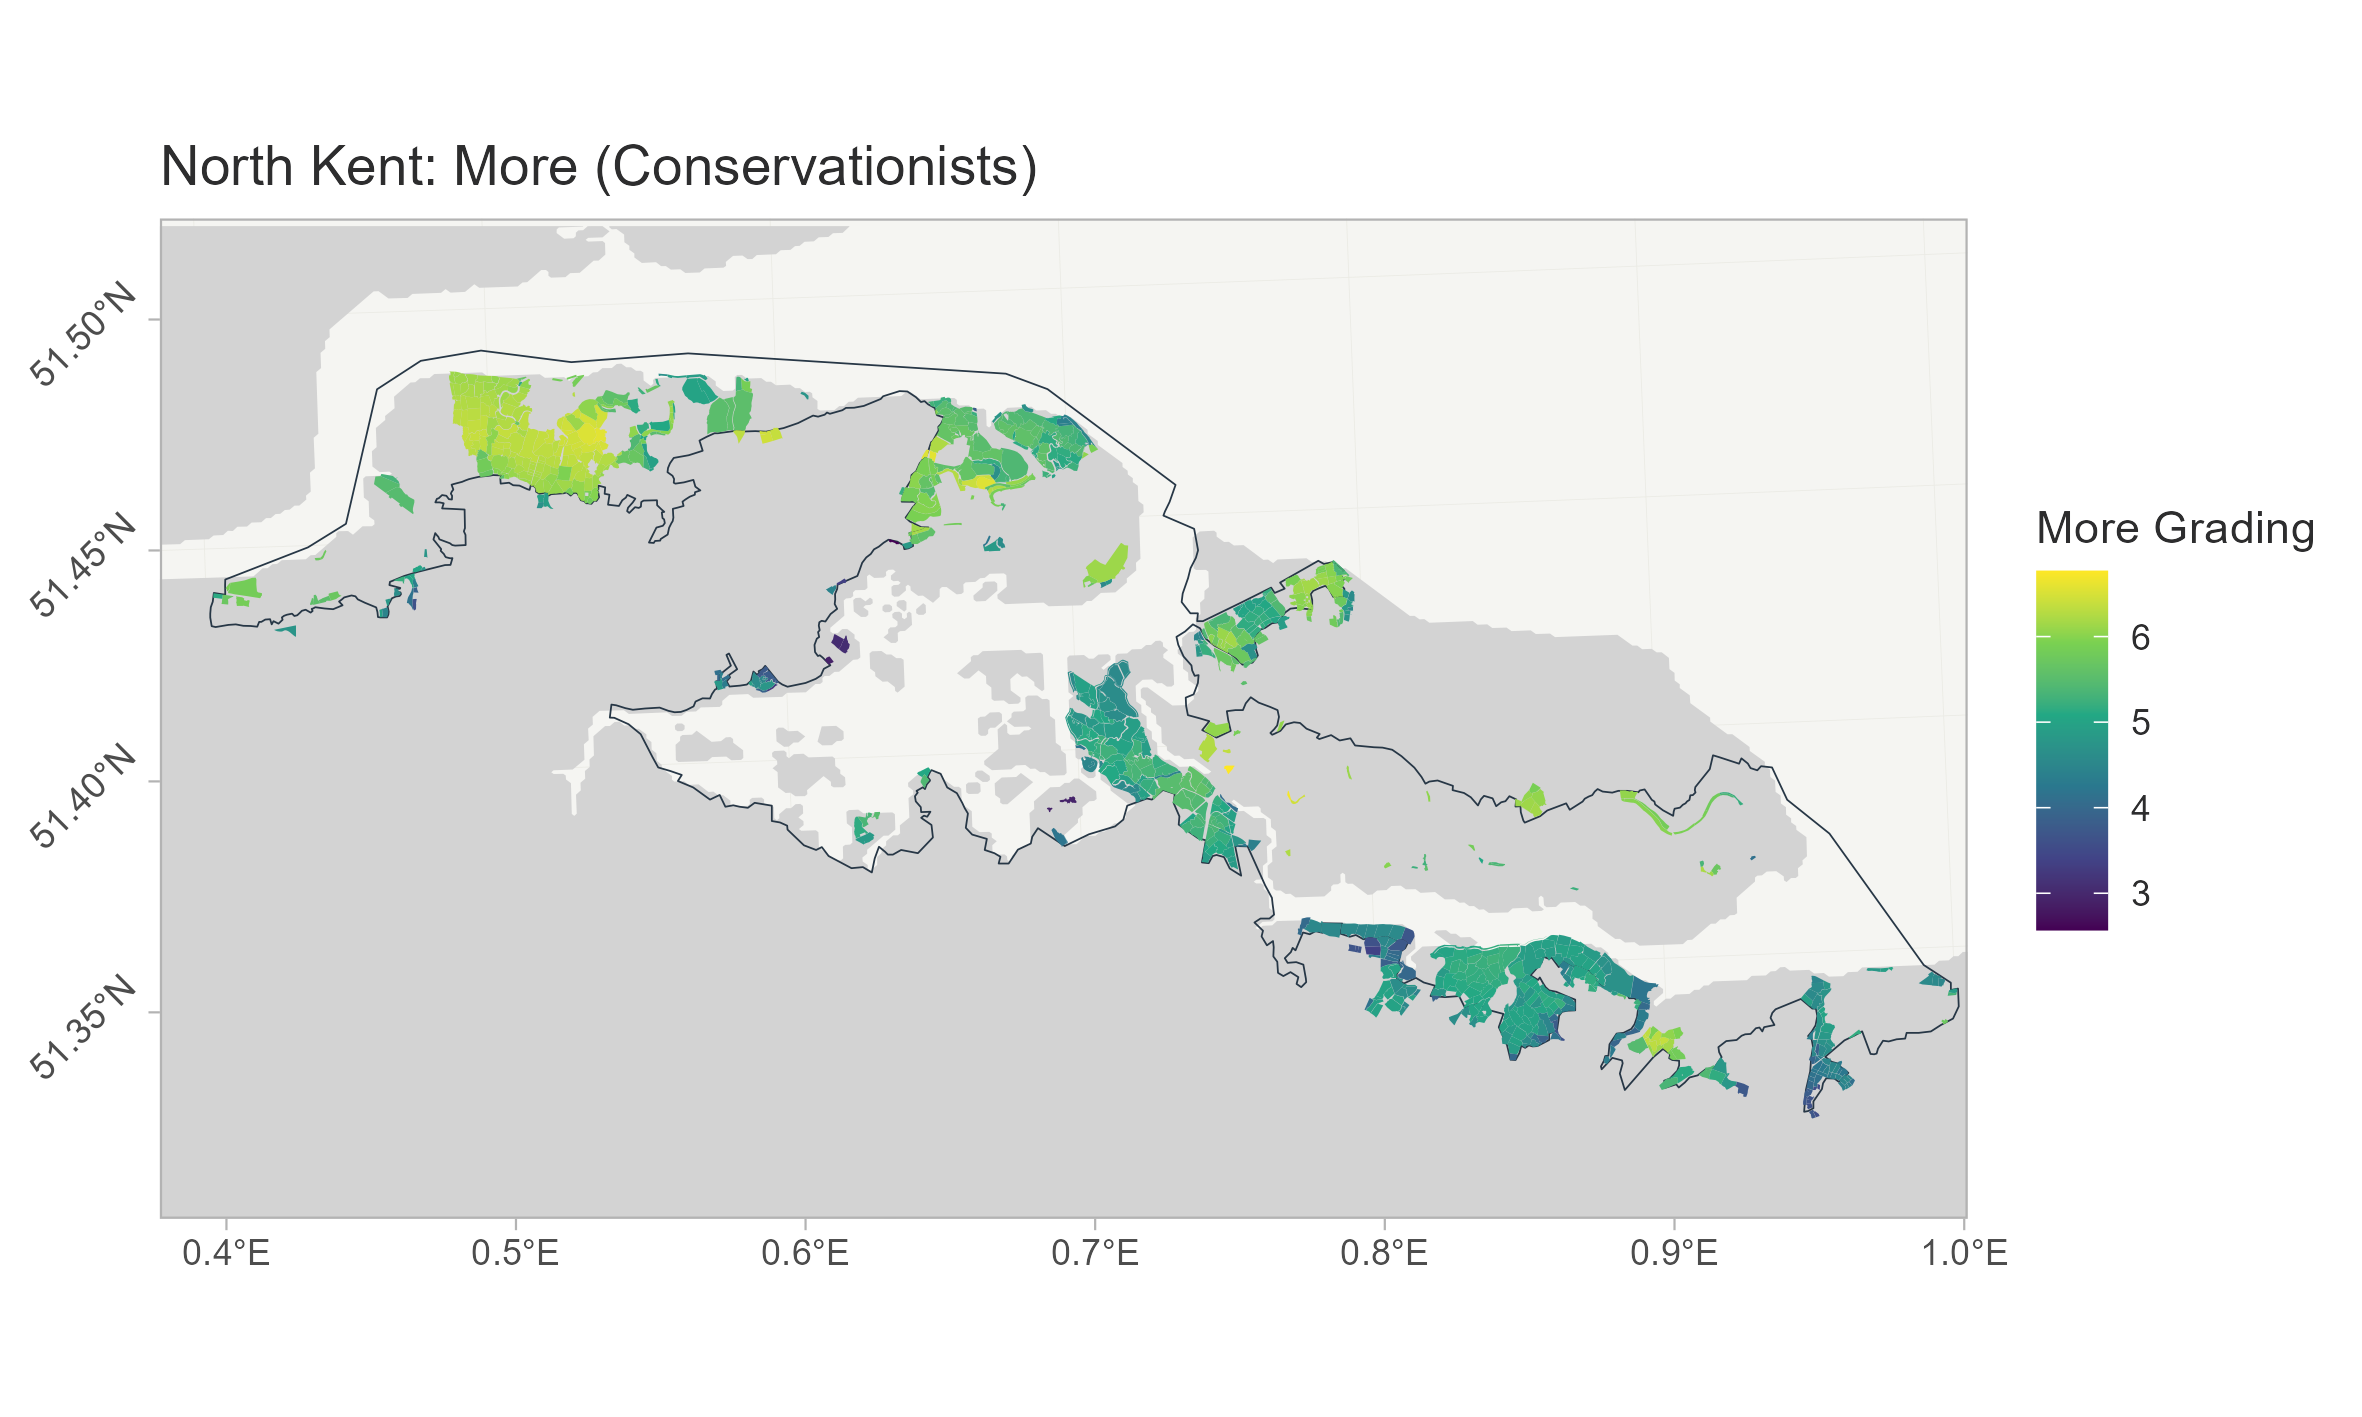
\includegraphics[width=7.29167in,height=\textheight]{Plots/NorthKent_G1_More.png}

}

\caption{\label{fig-NKMoreG1}Stakeholder gradings for group 1 in North
Kent for the more principle of nature restoration}

\end{figure}%

\begin{figure}[H]

\centering{

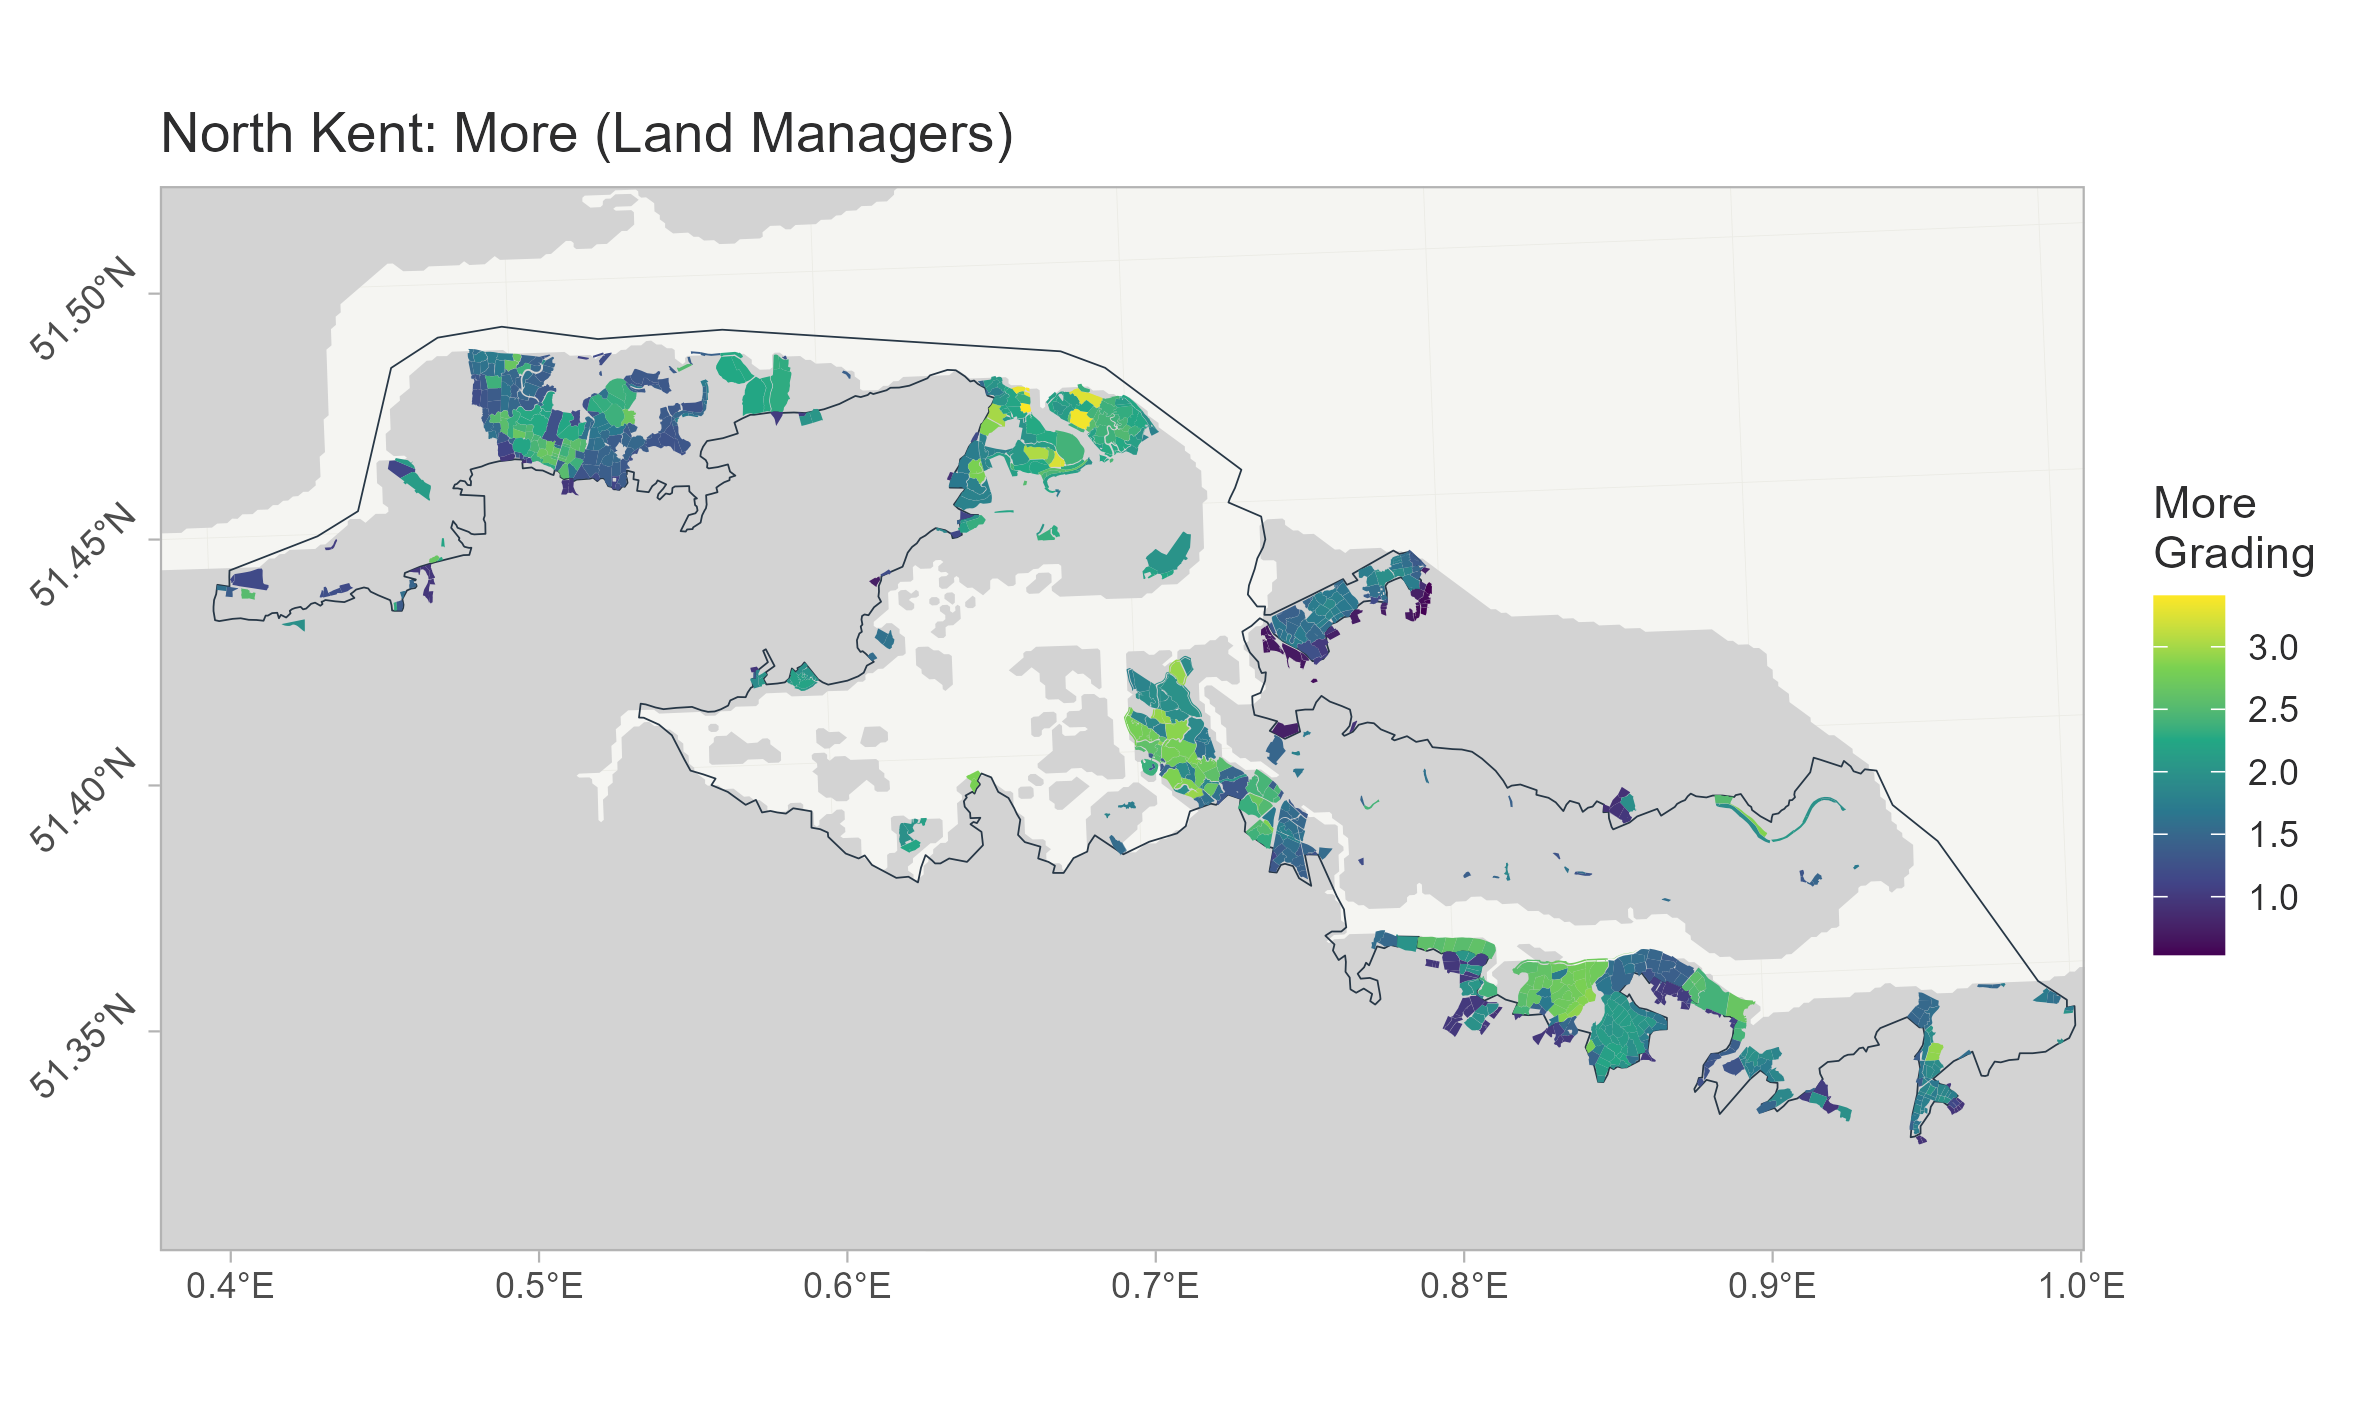
\includegraphics[width=7.29167in,height=\textheight]{Plots/NorthKent_G2_More.png}

}

\caption{\label{fig-NKMoreG2}Stakeholder gradings for group 2 in North
Kent for the more principle of nature restoration}

\end{figure}%

\newpage{}

\paragraph{North Kent: Arable Reversion for
Bigger}\label{north-kent-arable-reversion-for-bigger}

The stakeholder preferences for the reversion of arable land to lowland
wet grassland under the bigger principle of nature restoration for group
1 (Figure~\ref{fig-NKArBigG1}) and group 2 (Figure~\ref{fig-NKArBigG2}).
Note: during the stakeholder workshops no guidelines or masks were
created specifically for arable reversion.

\begin{figure}[H]

\centering{

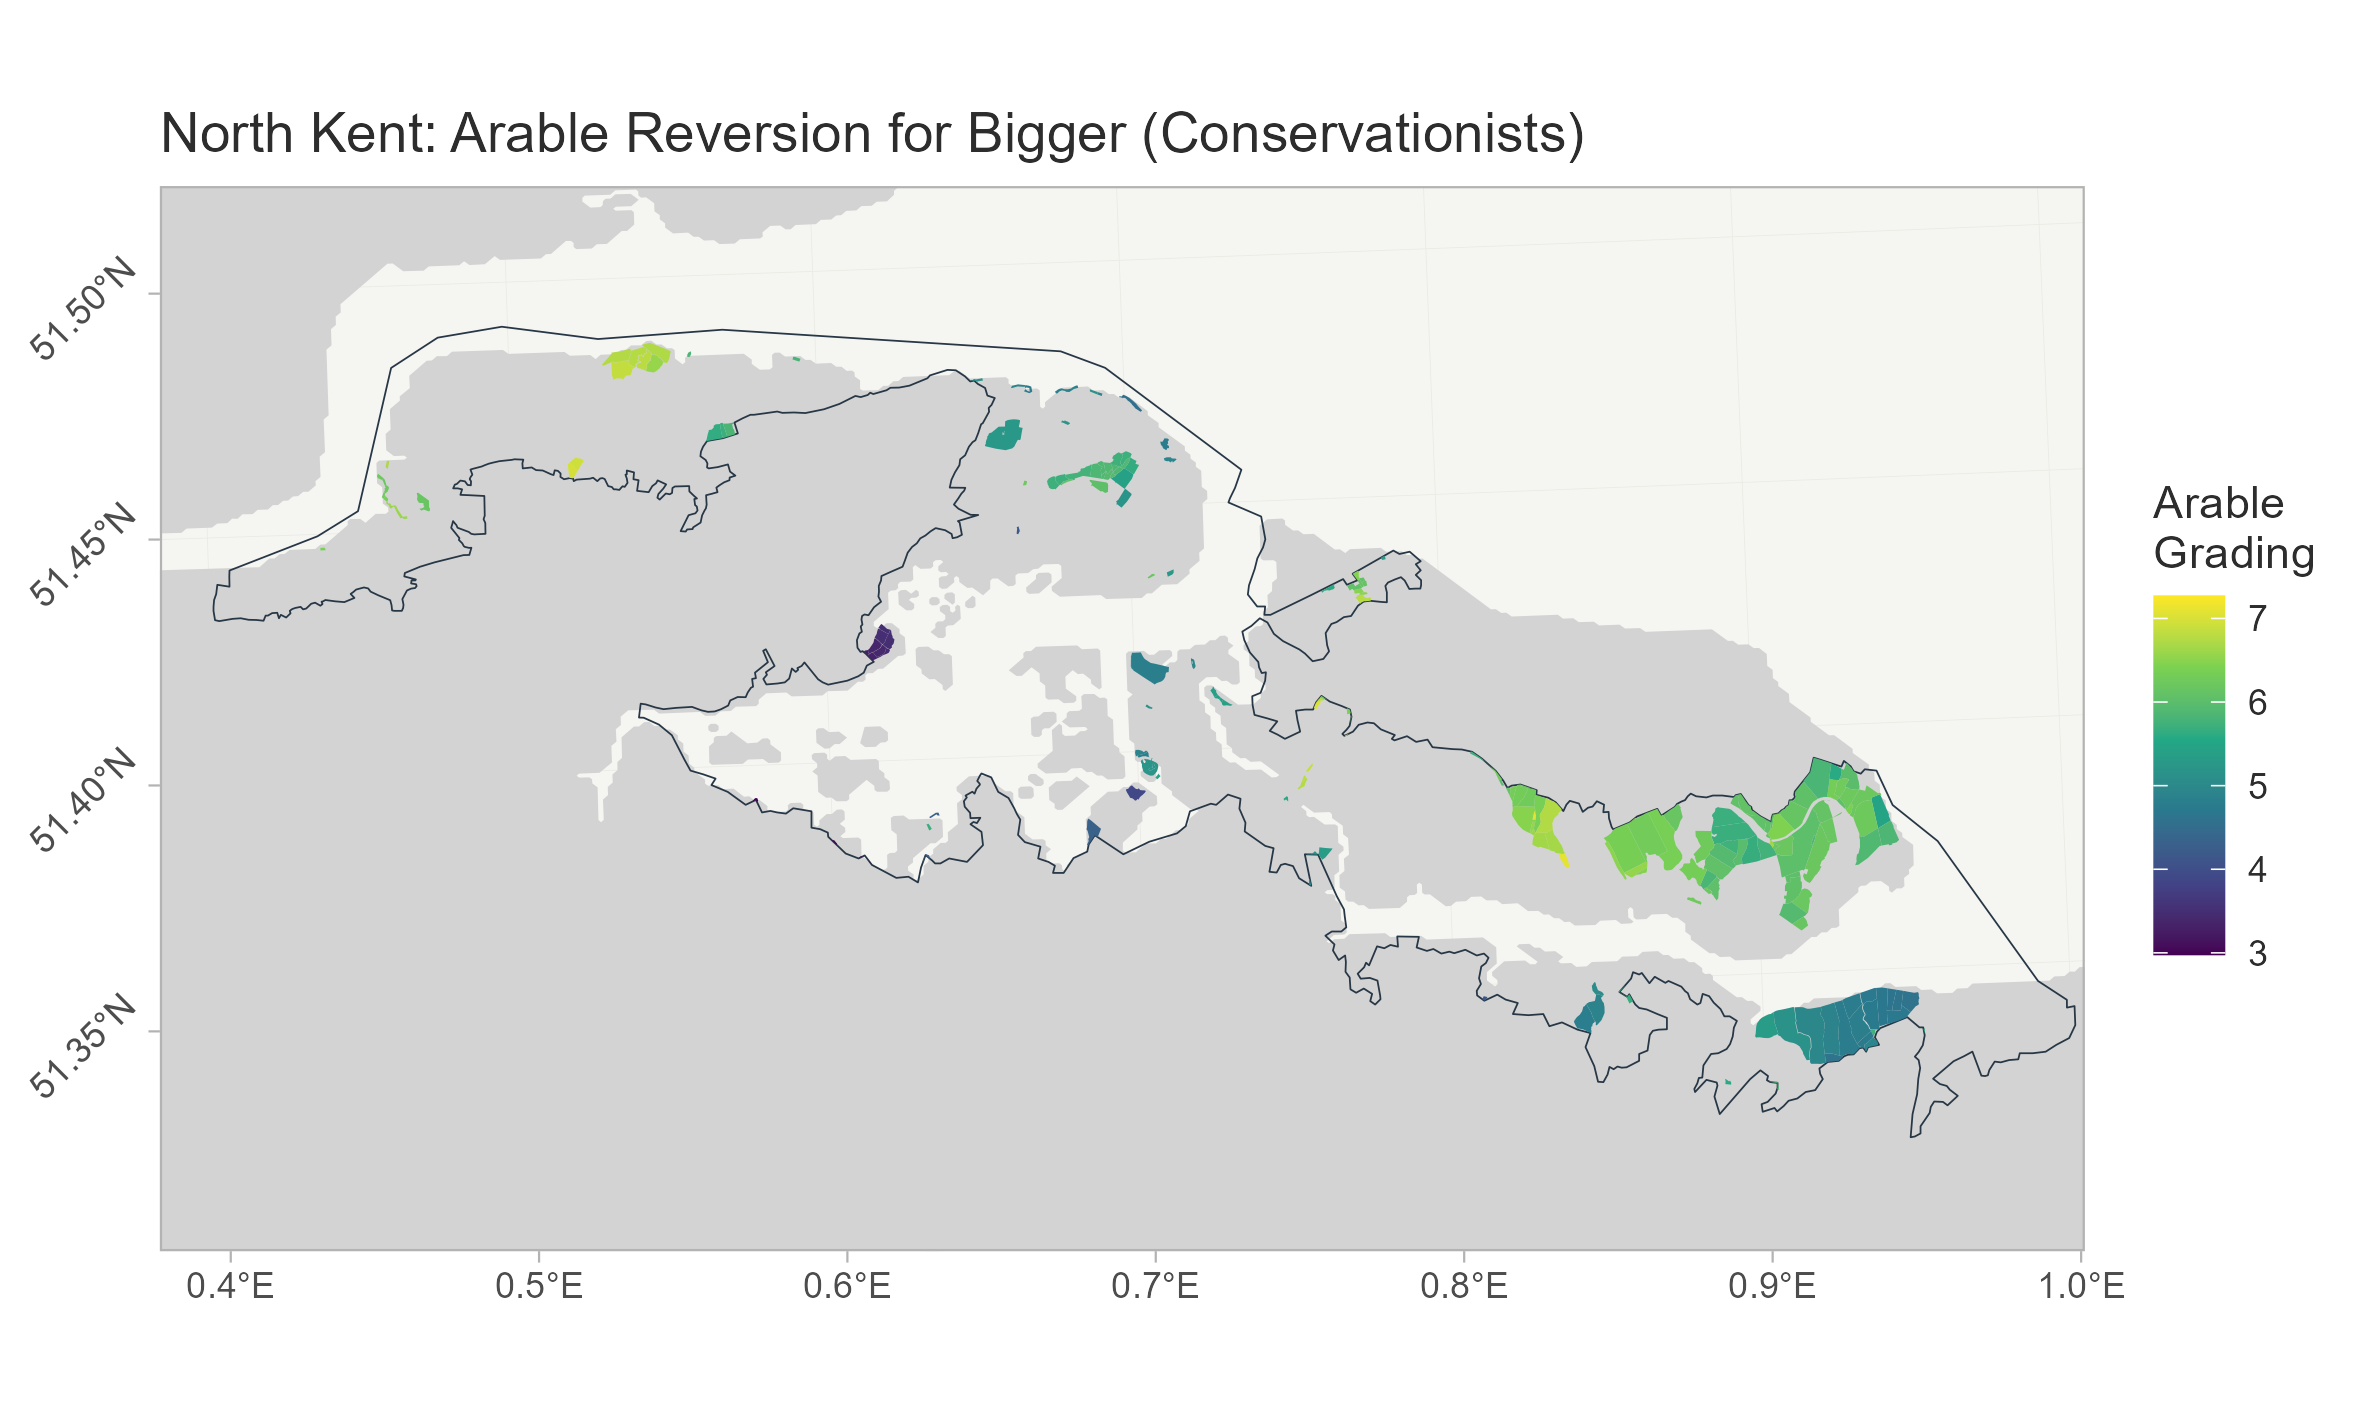
\includegraphics[width=7.29167in,height=\textheight]{Plots/NorthKent_G1_ArableBig.png}

}

\caption{\label{fig-NKArBigG1}Stakeholder gradings for group 1 in North
Kent for the reversion of arable land to lowland wet grassland under the
bigger principle of nature restoration}

\end{figure}%

\begin{figure}[H]

\centering{

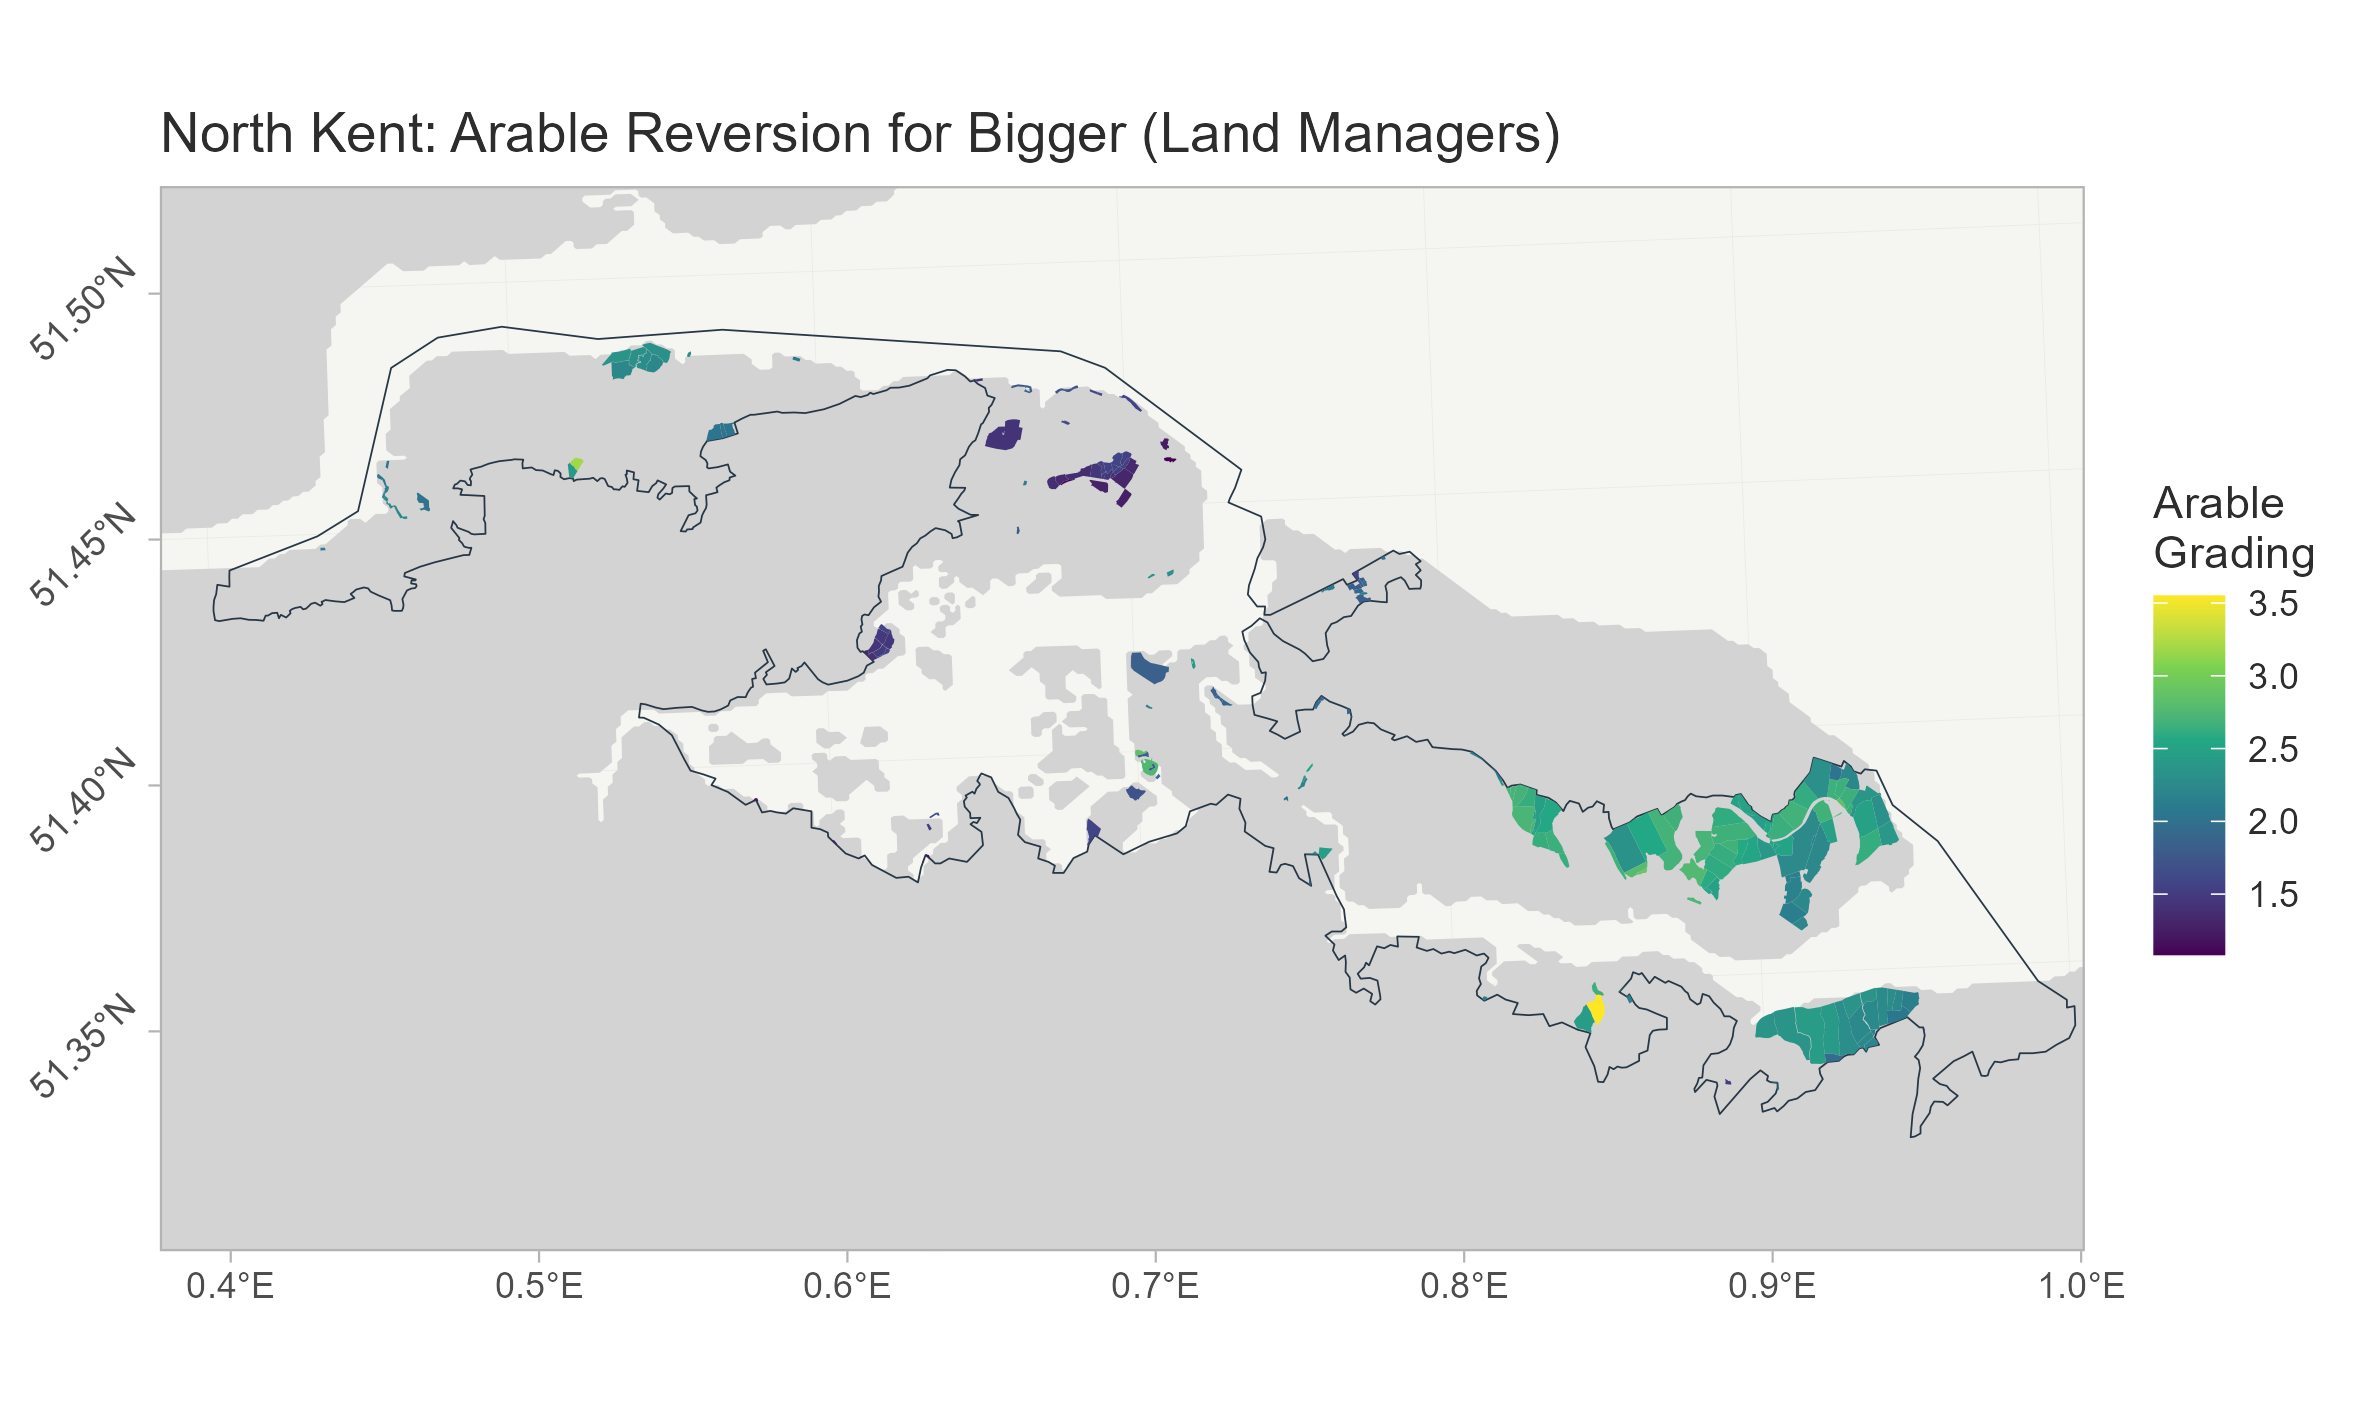
\includegraphics[width=7.29167in,height=\textheight]{Plots/NorthKent_G2_ArableBig.png}

}

\caption{\label{fig-NKArBigG2}Stakeholder gradings for group 2 in North
Kent for the reversion of arable land to lowland wet grassland under the
bigger principle of nature restoration}

\end{figure}%

\newpage{}

\paragraph{North Kent: Arable Reversion for
More}\label{north-kent-arable-reversion-for-more}

The stakeholder preferences for the reversion of arable land to lowland
wet grassland under the more principle of nature restoration for group 1
(Figure~\ref{fig-NKArMoreG1}) and group 2 (Figure~\ref{fig-NKArMoreG2}).
Note: during the stakeholder workshops no guidelines or masks were
created specifically for arable reversion.

\begin{figure}[H]

\centering{

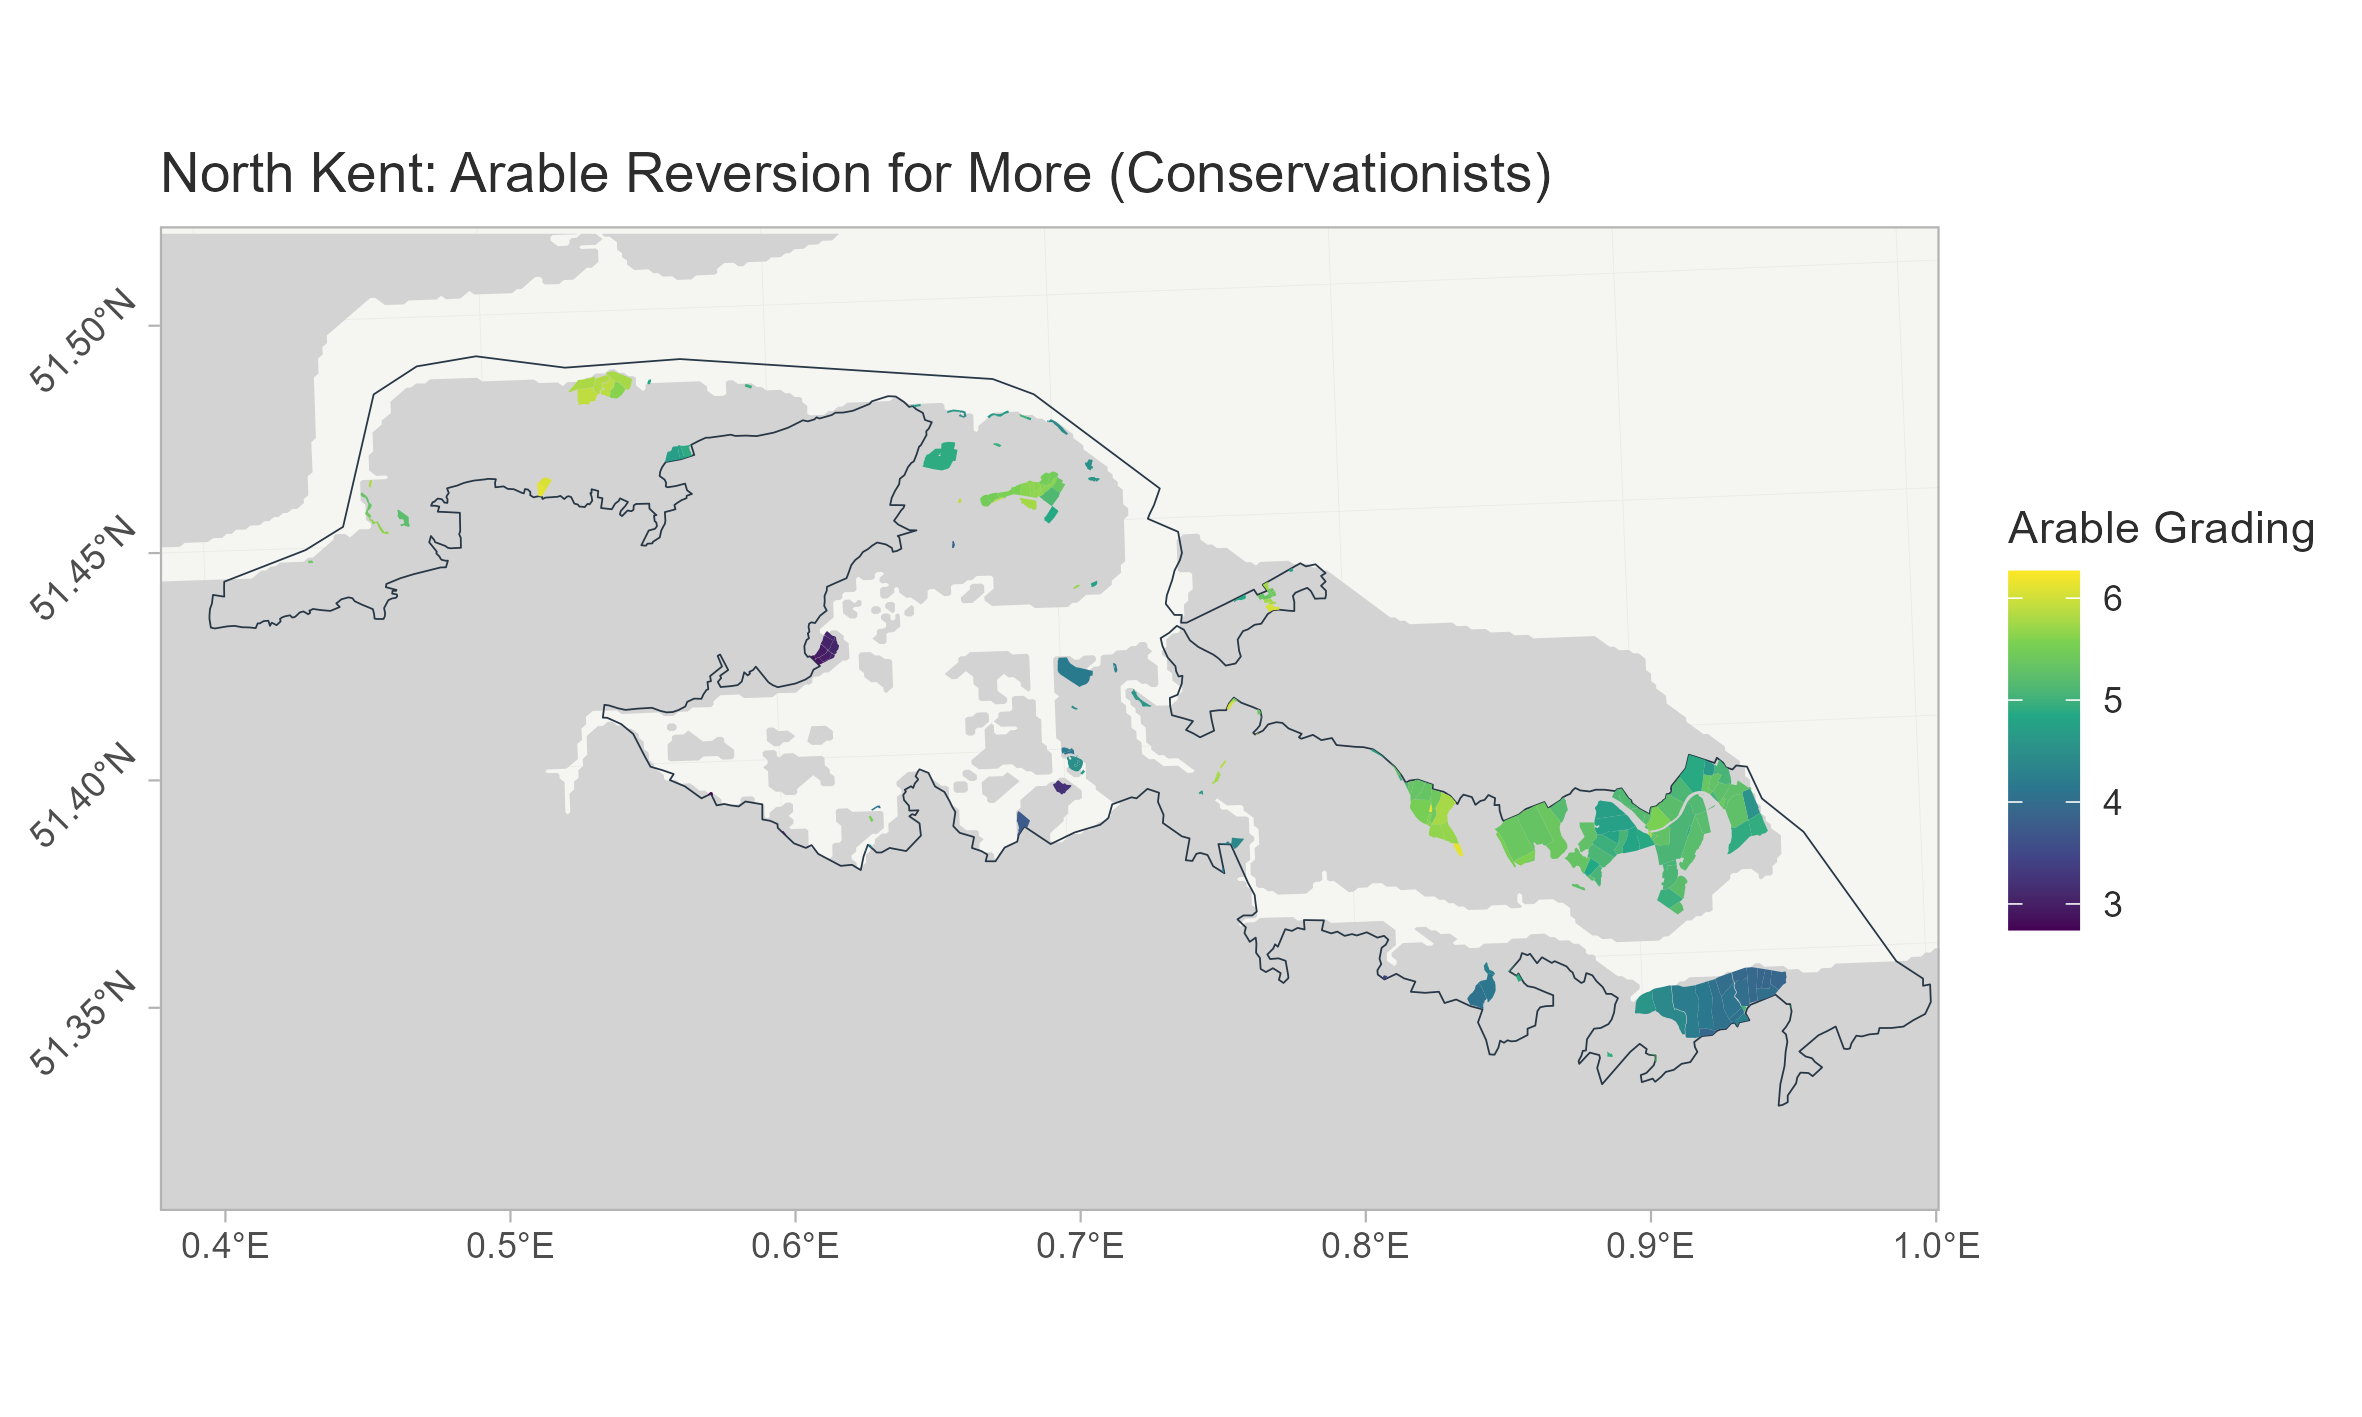
\includegraphics[width=7.29167in,height=\textheight]{Plots/NorthKent_G1_ArableMore.png}

}

\caption{\label{fig-NKArMoreG1}Stakeholder gradings for group 1 in North
Kent for the reversion of arable land to lowland wet grassland under the
bigger principle of nature restoration}

\end{figure}%

\begin{figure}[H]

\centering{

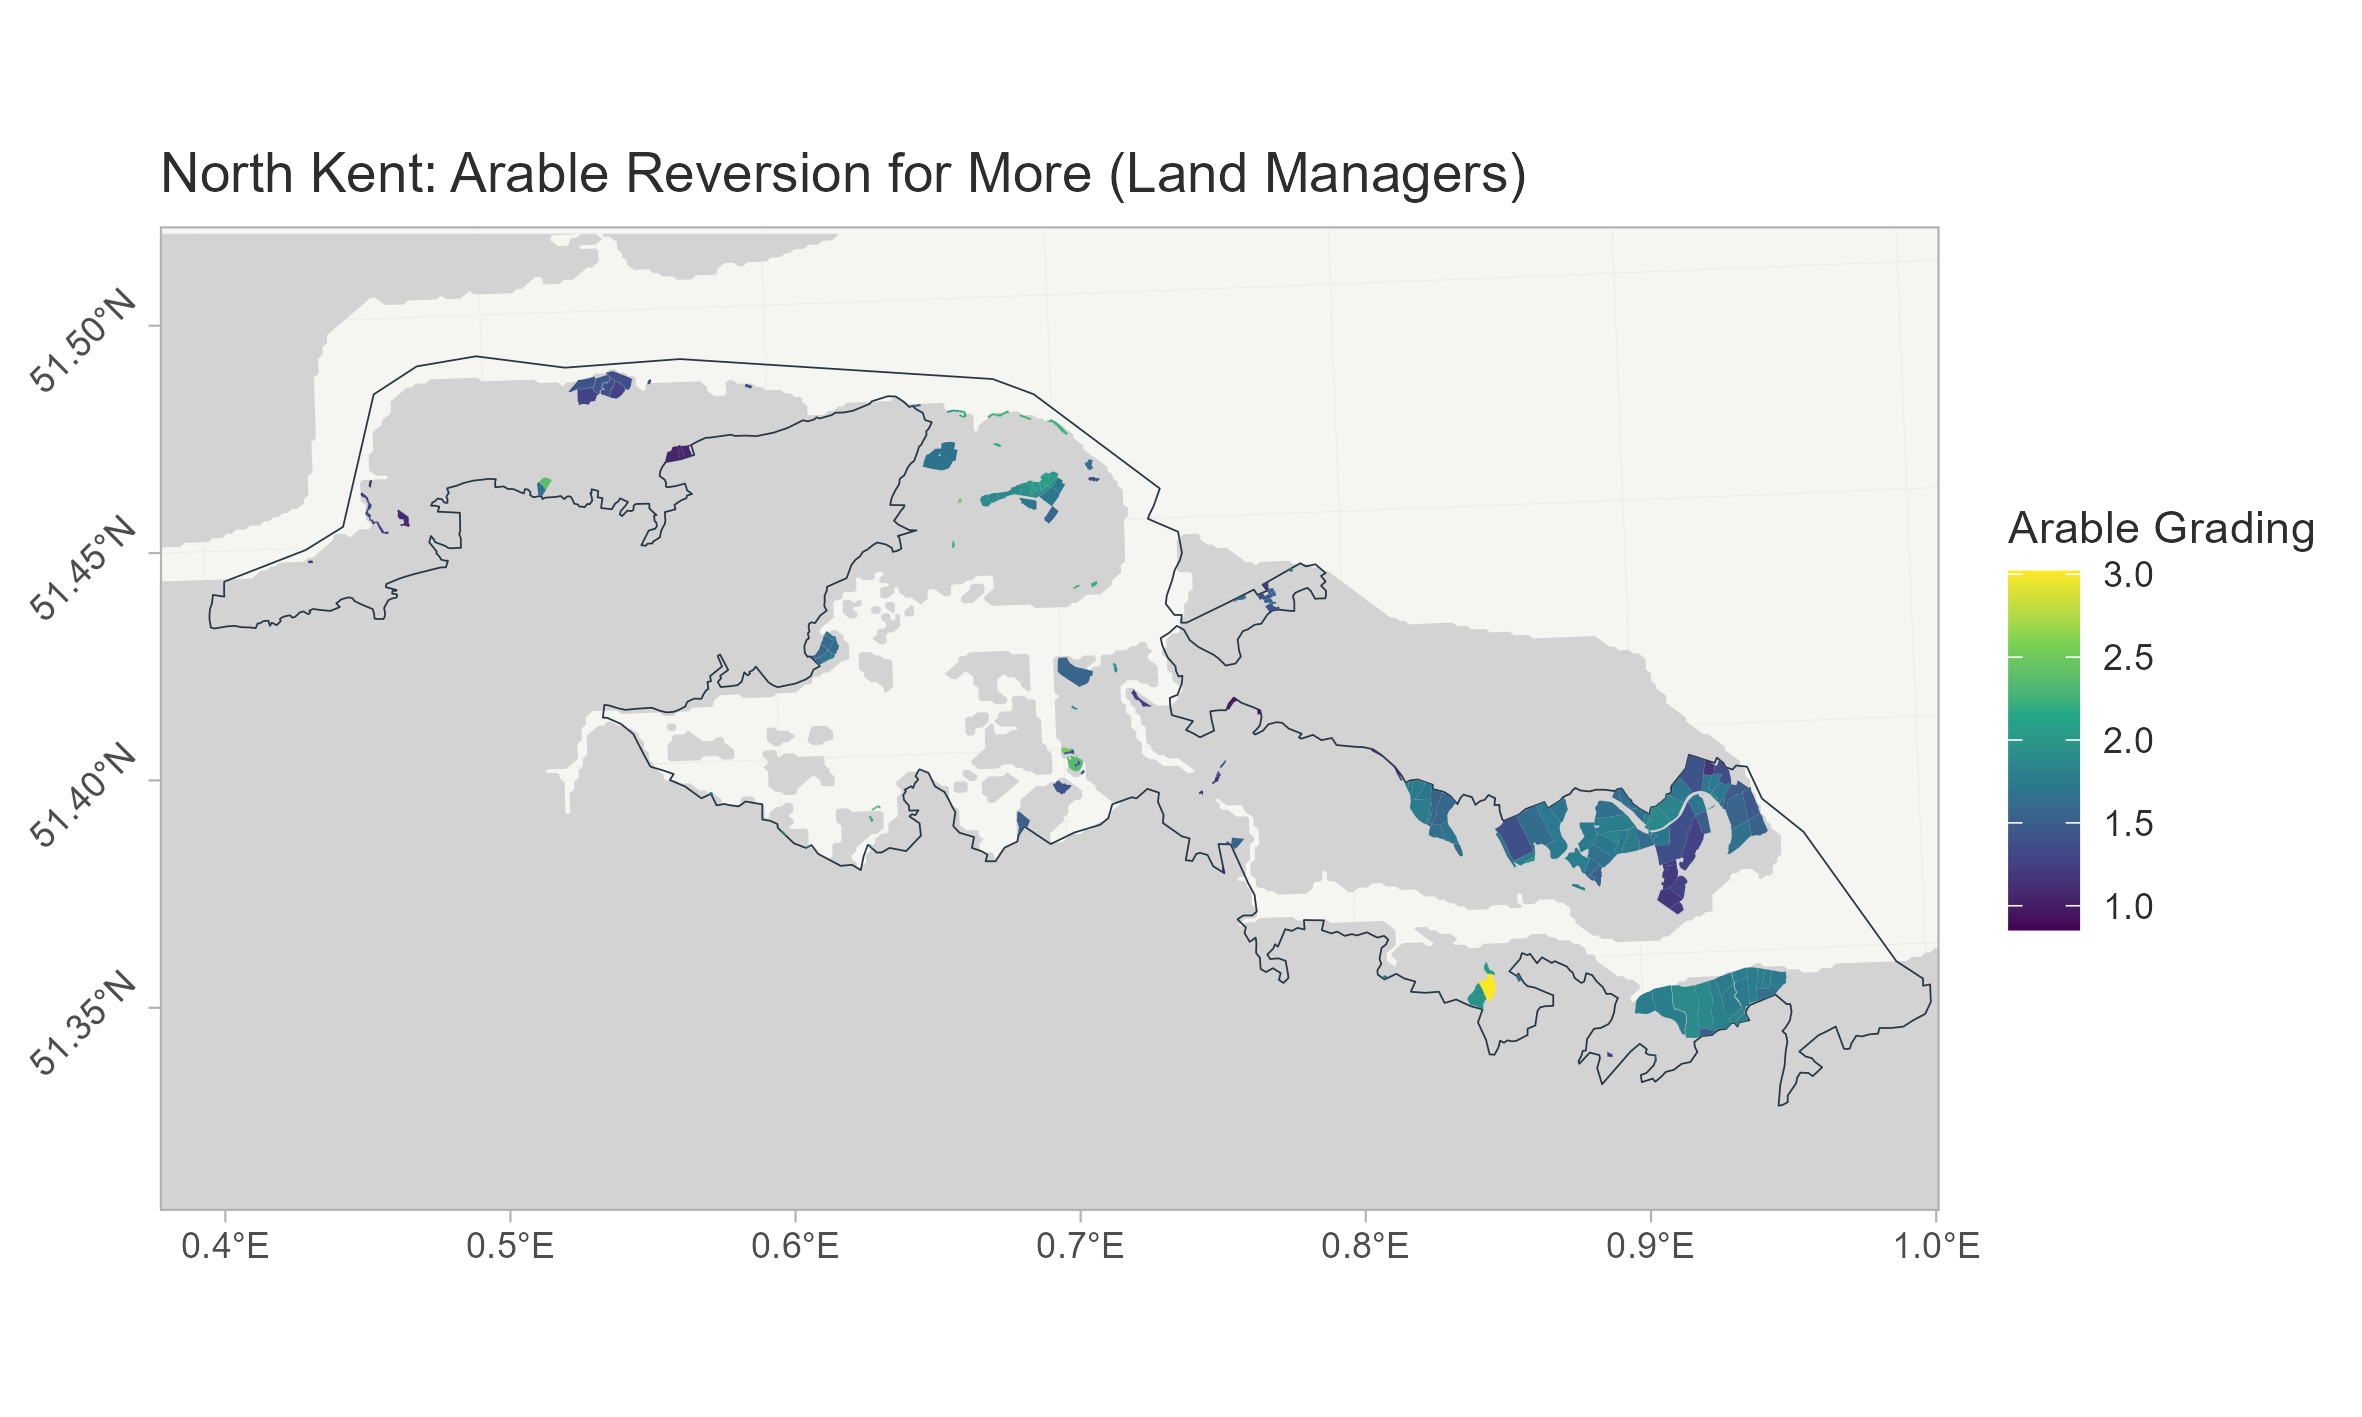
\includegraphics[width=7.29167in,height=\textheight]{Plots/NorthKent_G2_ArableMore.png}

}

\caption{\label{fig-NKArMoreG2}Stakeholder gradings for group 2 in North
Kent for the reversion of arable land to lowland wet grassland under the
bigger principle of nature restoration}

\end{figure}%

\newpage{}

\subsubsection{Essex Results}\label{essex-results}

For Essex we had two different stakeholder groups. Group 1 (G1) was a
group of conservationists and group 2 was a group of landowners and
farmers.

\paragraph{Essex: Better}\label{essex-better}

The stakeholder preferences for the better principle of nature
restoration for group 1 and group 2 can be visualized in
(Figure~\ref{fig-EsBetterG1}) and (Figure~\ref{fig-EsBetterG2}),
receptively. The stakeholder guidelines that were used to produce these
maps can be found in Table~\ref{tbl-EsG1} for group 1 and
Table~\ref{tbl-EsG2} for group 2.

\begin{figure}[H]

\centering{

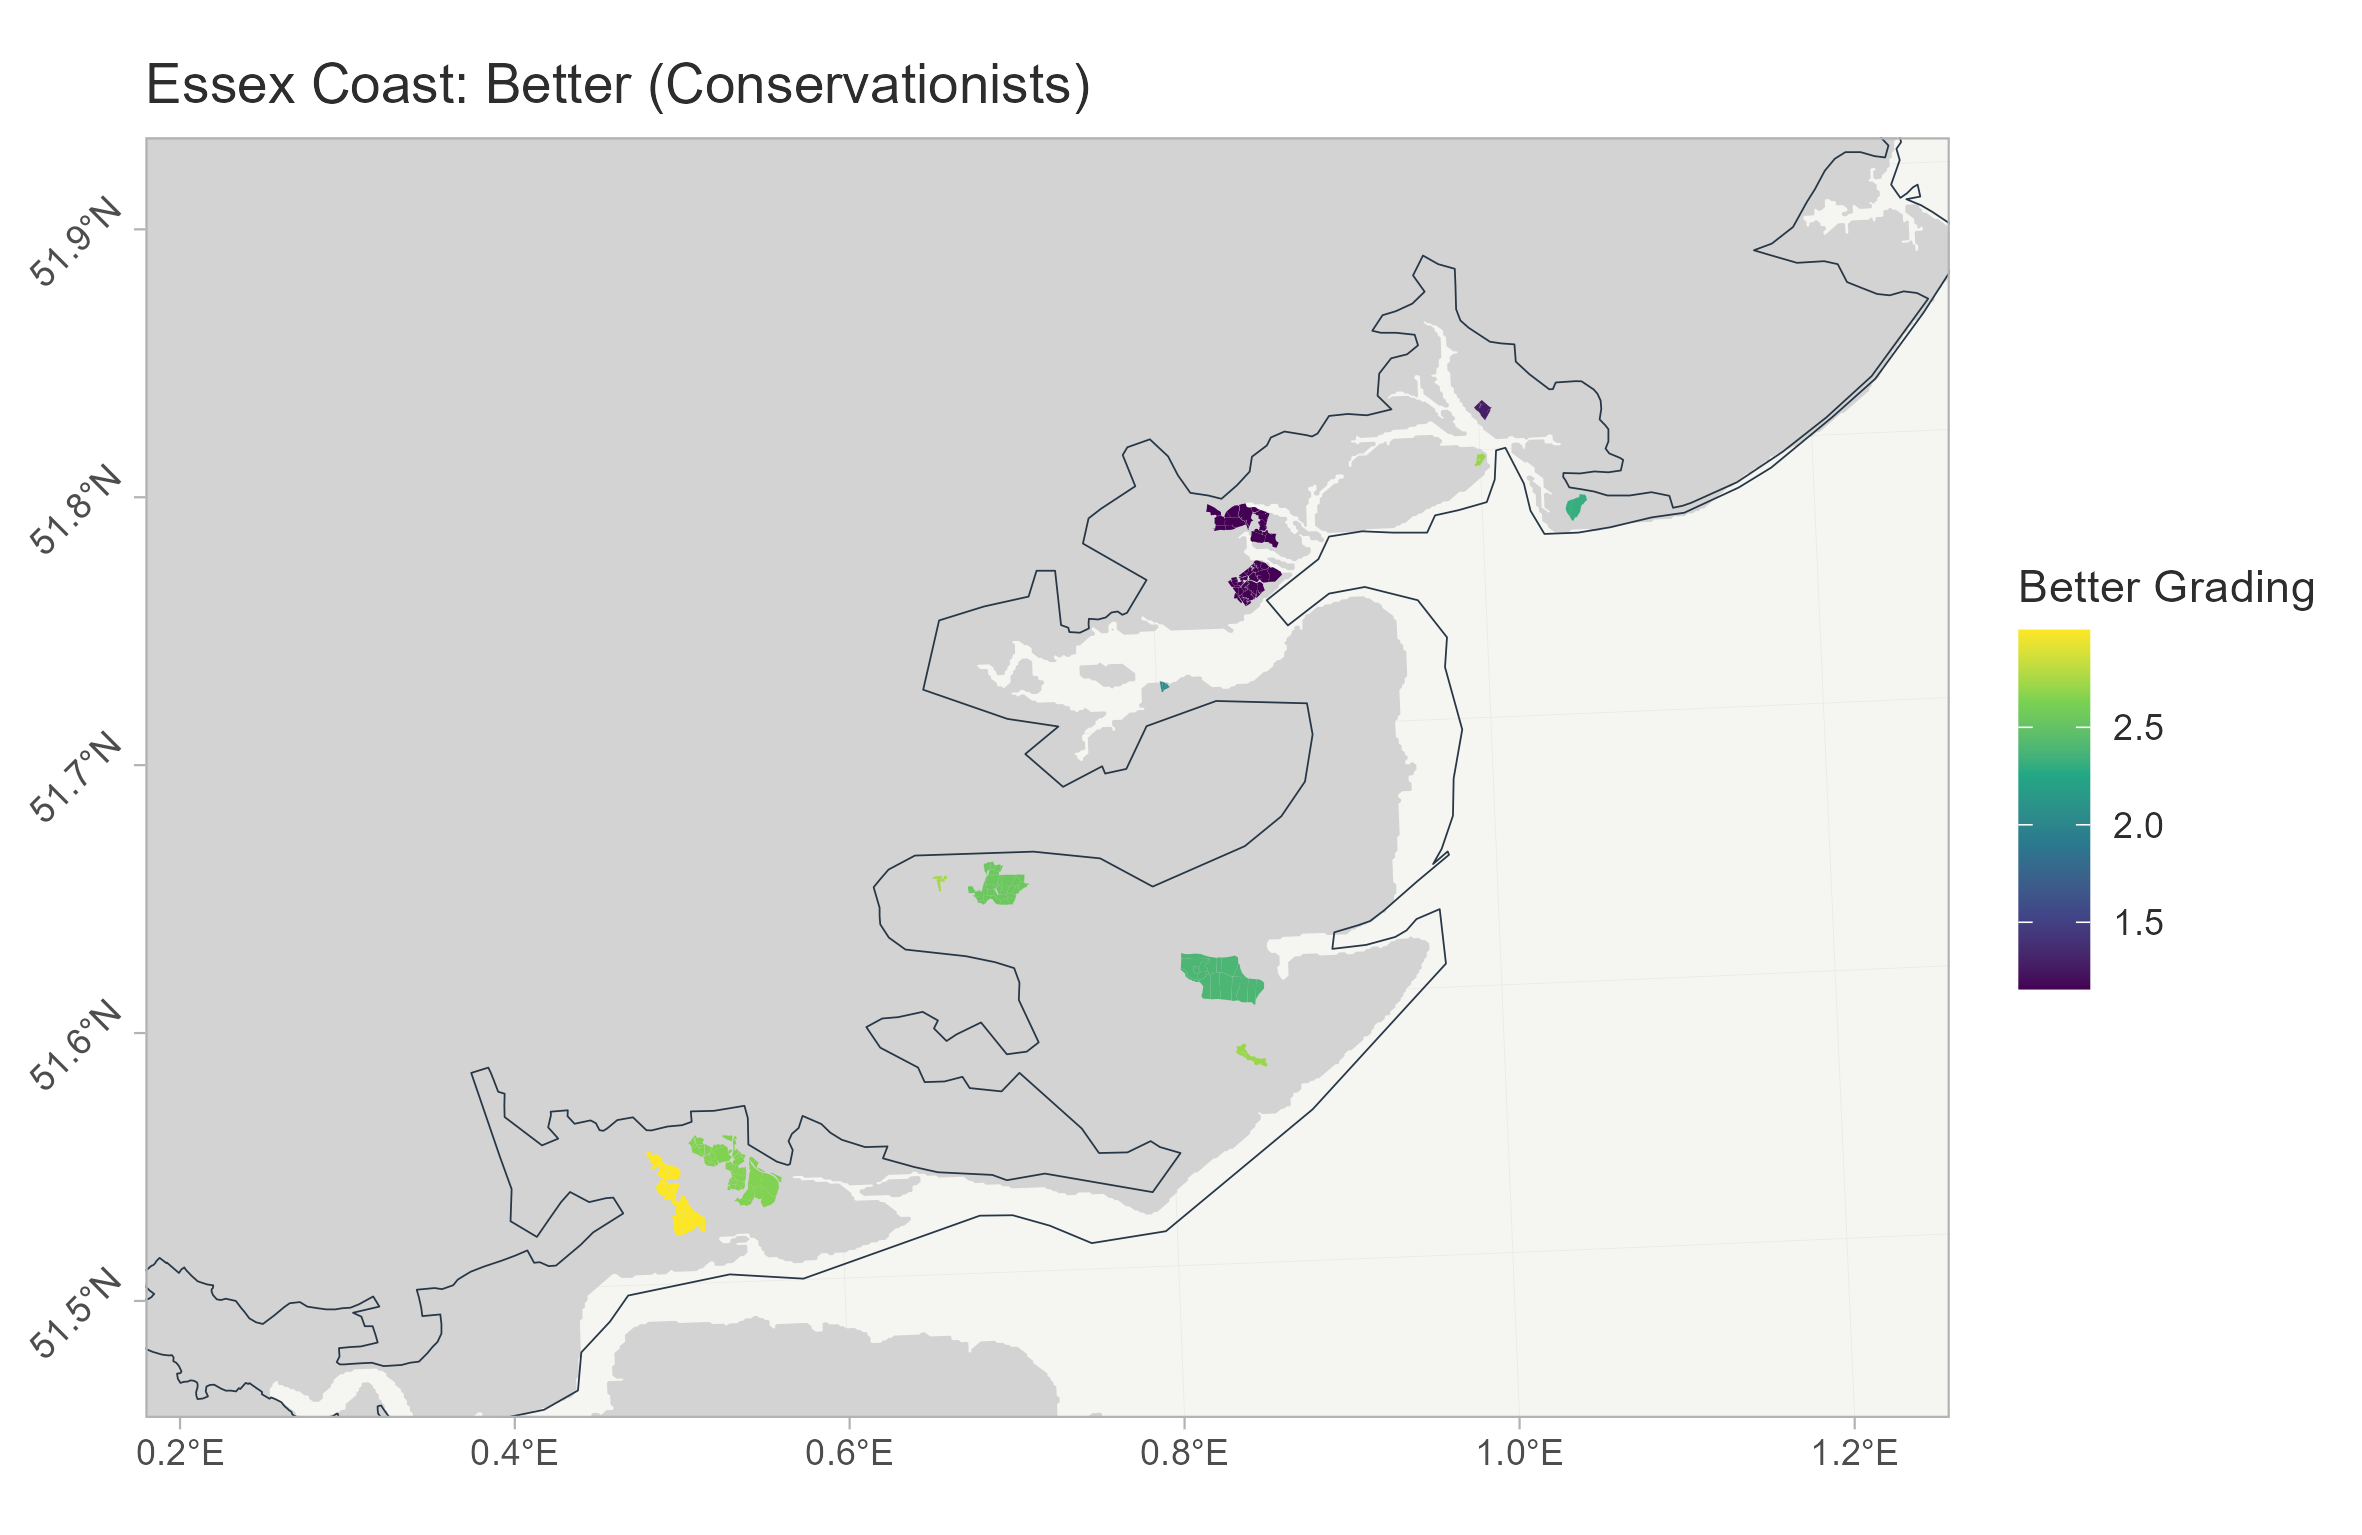
\includegraphics[width=7.29167in,height=\textheight]{Plots/Essex_G1_Better.png}

}

\caption{\label{fig-EsBetterG1}Stakeholder gradings for group 1 in Essex
for the better principle of nature restoration}

\end{figure}%

\begin{figure}[H]

\centering{

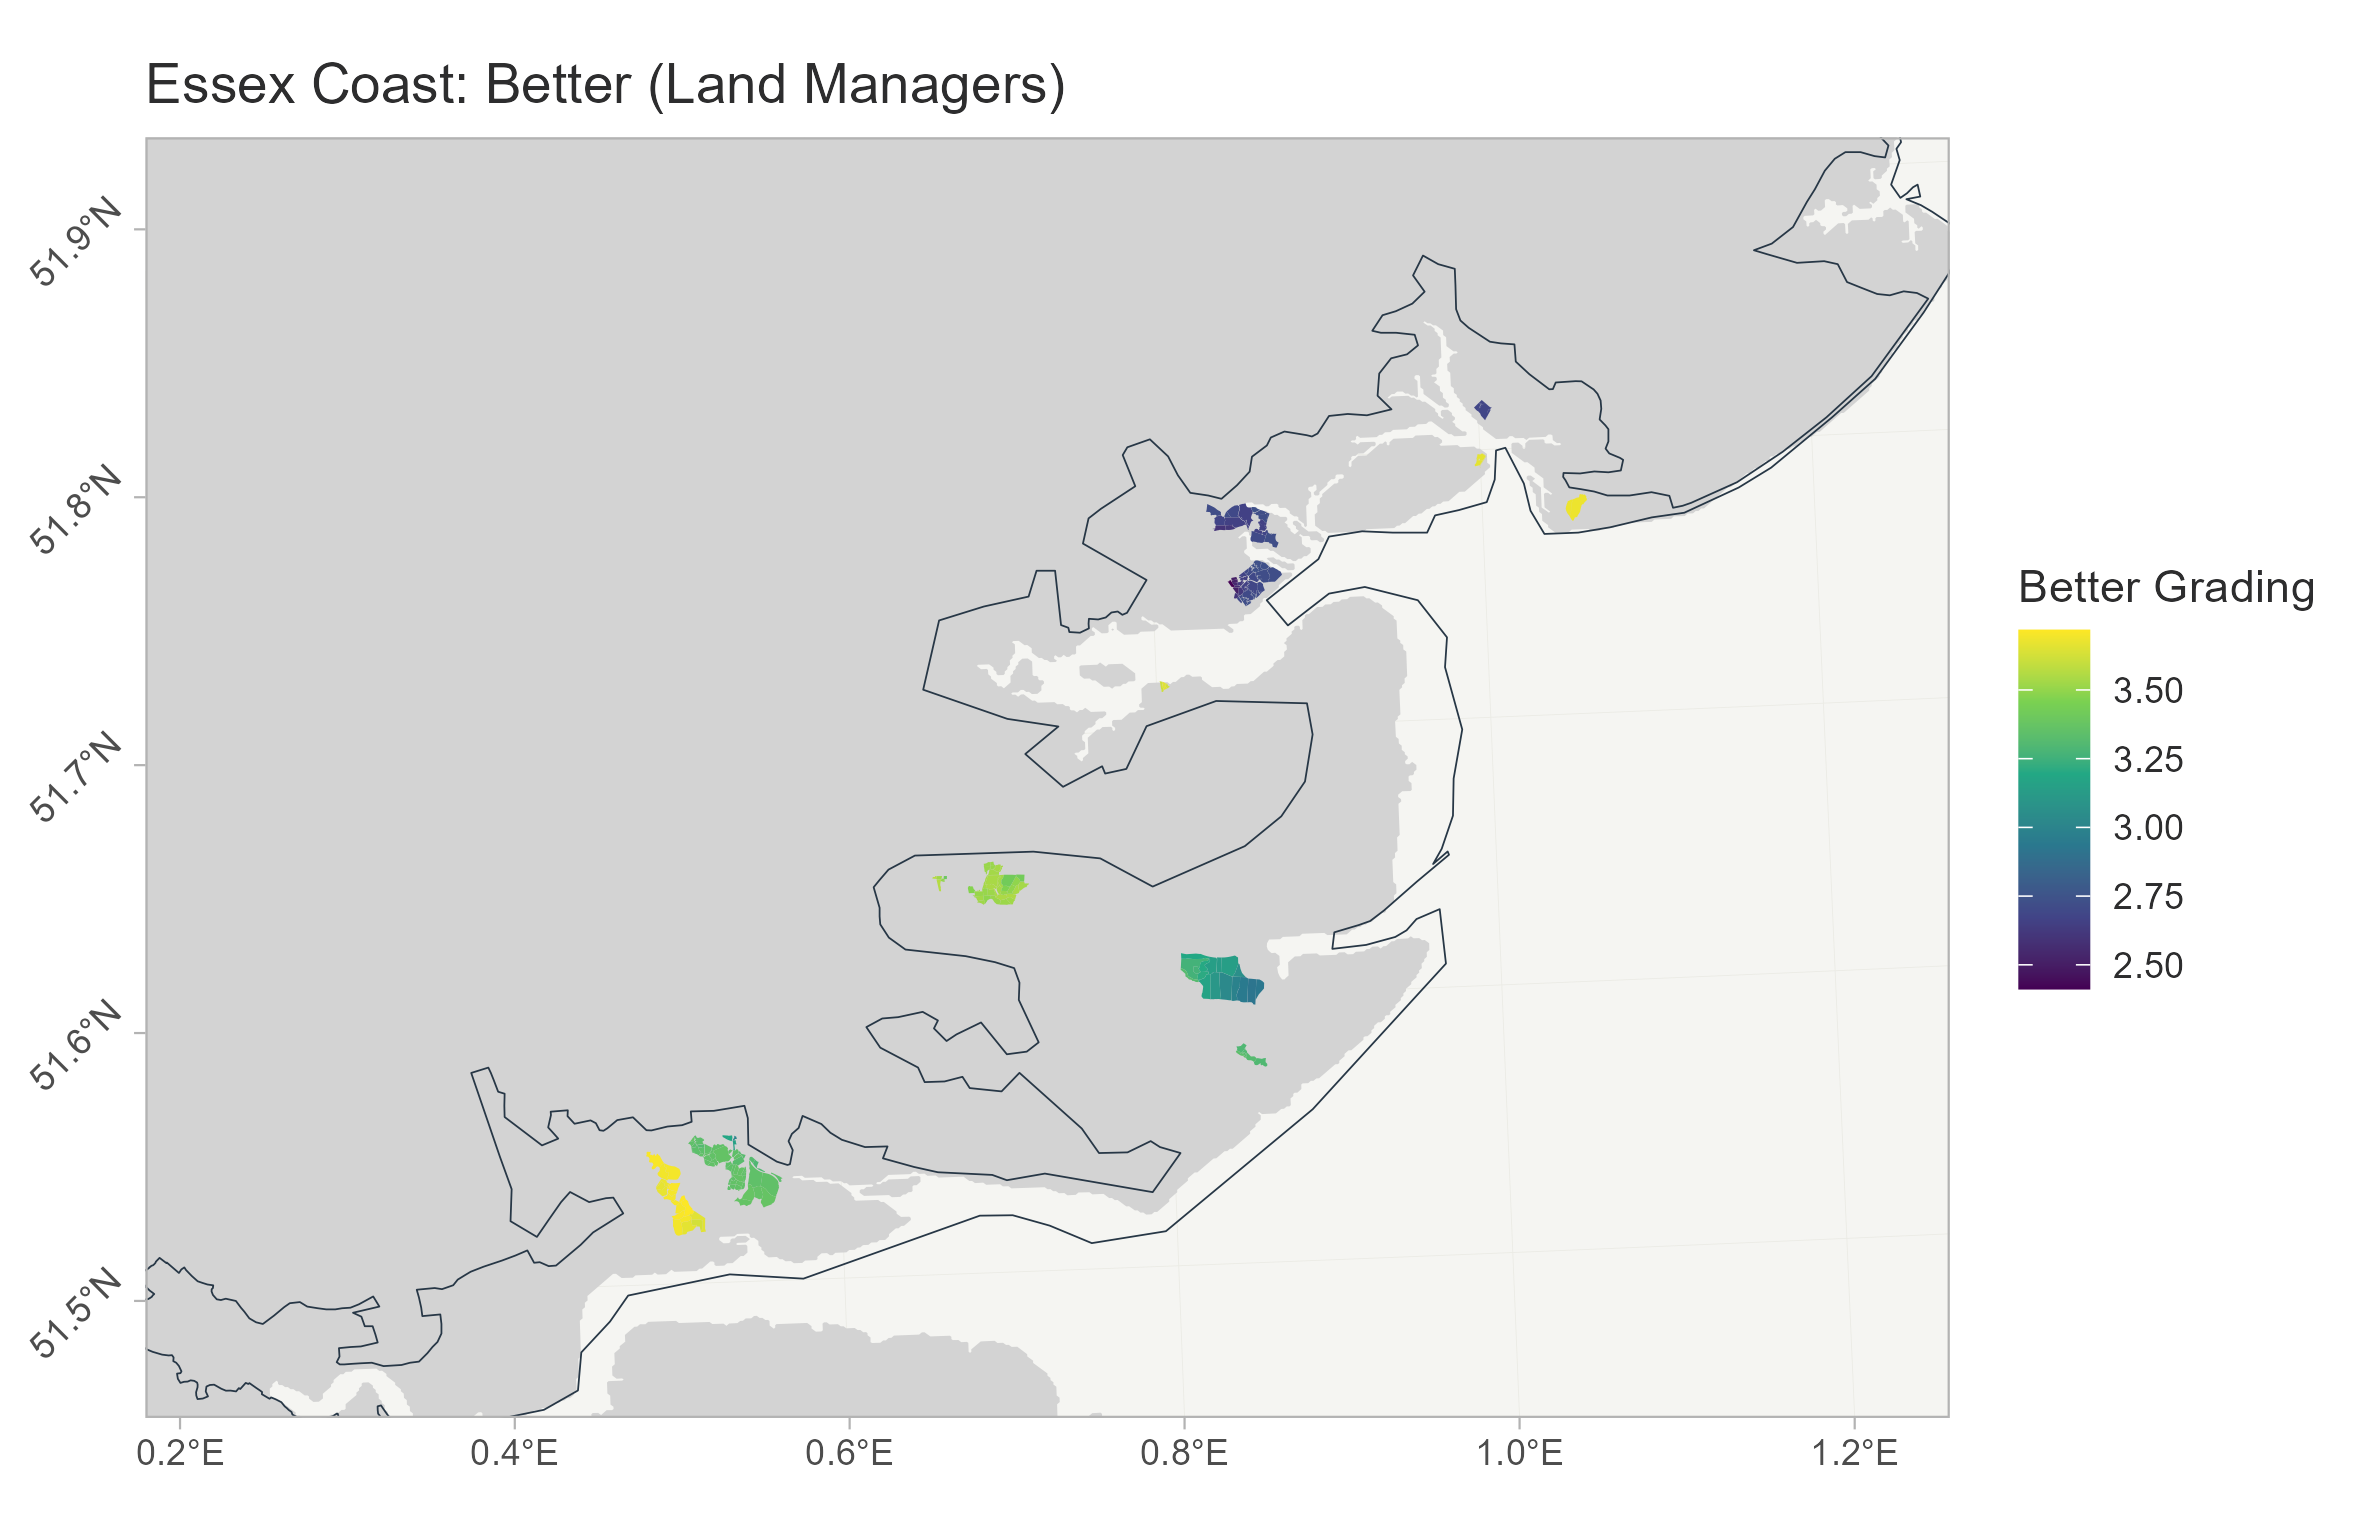
\includegraphics[width=7.29167in,height=\textheight]{Plots/Essex_G2_Better.png}

}

\caption{\label{fig-EsBetterG2}Stakeholder gradings for group 2 in Essex
for the better principle of nature restoration}

\end{figure}%

\newpage{}

\paragraph{Essex: Bigger}\label{essex-bigger}

The stakeholder preferences for the bigger principle of nature
restoration for group 1 (Figure~\ref{fig-EsBigG1}) and 2
(Figure~\ref{fig-EsBigG2}).

\begin{figure}[H]

\centering{

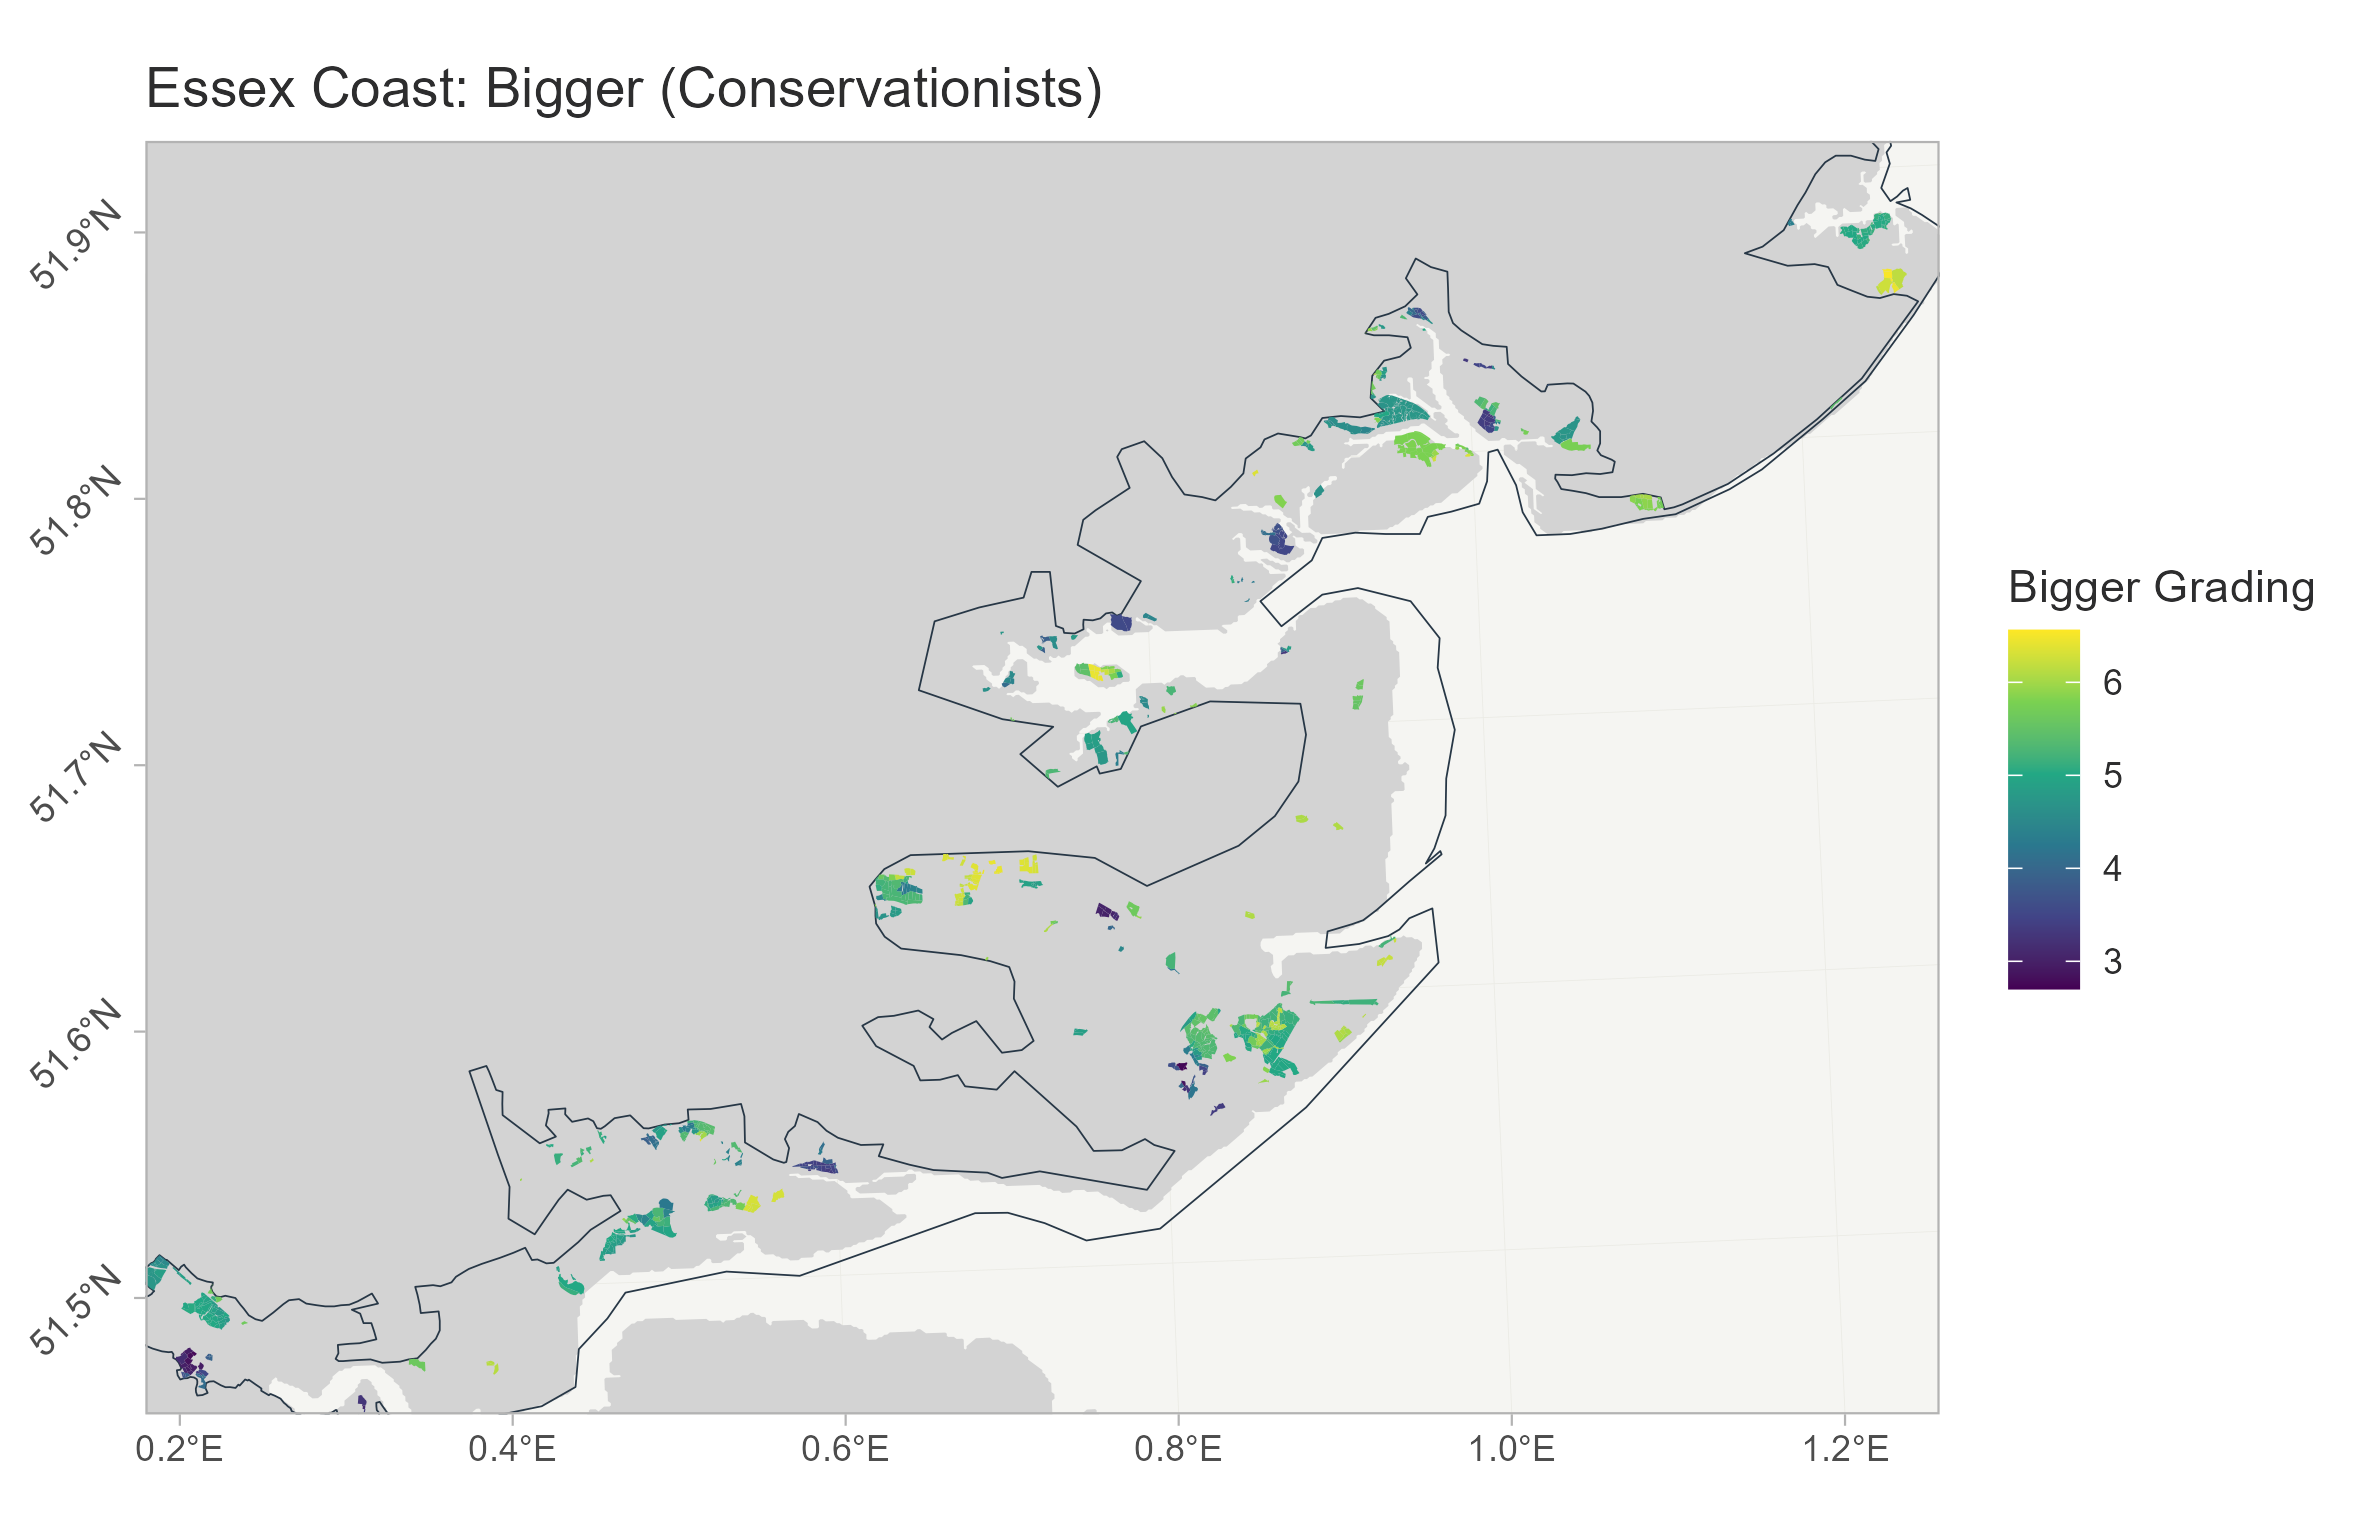
\includegraphics[width=7.29167in,height=\textheight]{Plots/Essex_G1_Bigger.png}

}

\caption{\label{fig-EsBigG1}Stakeholder gradings for group 1 in Essex
for the bigger principle of nature restoration}

\end{figure}%

\begin{figure}[H]

\centering{

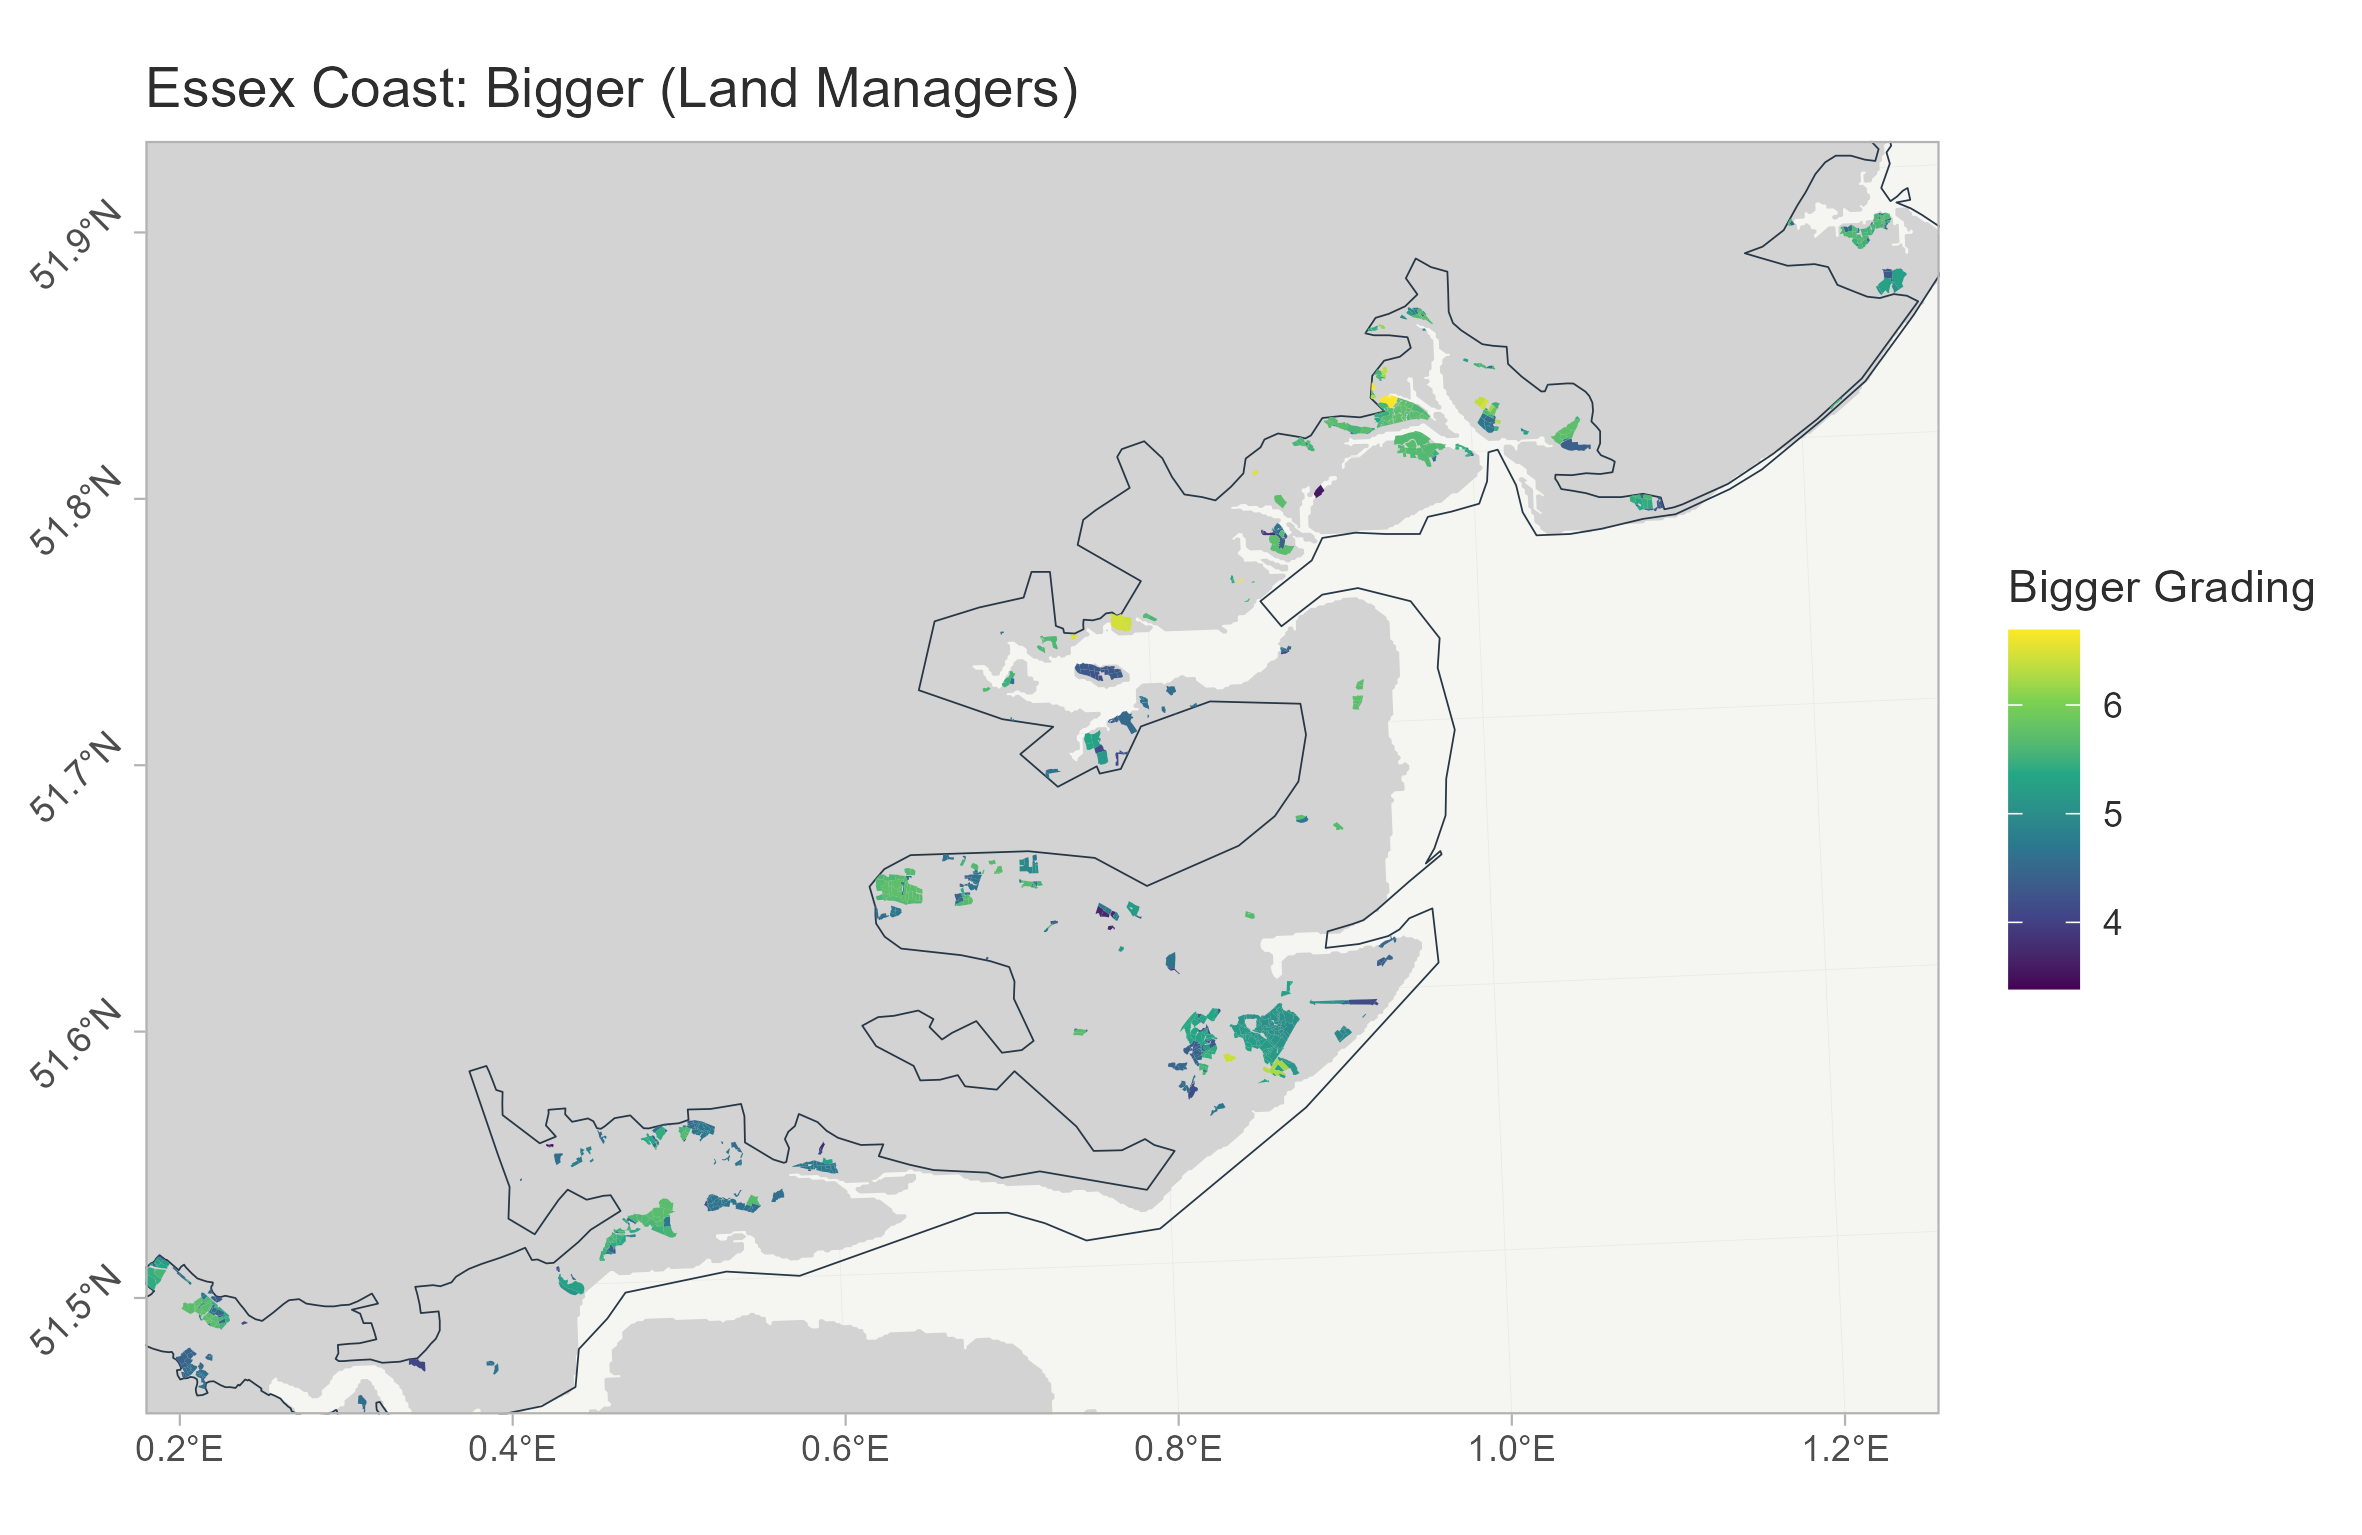
\includegraphics[width=7.29167in,height=\textheight]{Plots/Essex_G2_Bigger.png}

}

\caption{\label{fig-EsBigG2}Stakeholder gradings for group 2 in Essex
for the bigger principle of nature restoration}

\end{figure}%

\newpage{}

\paragraph{Essex: More}\label{essex-more}

The stakeholder preferences for the more principle of nature restoration
for group 1 (Figure~\ref{fig-EsMoreG1}) and 2
(Figure~\ref{fig-EsMoreG2}).

\begin{figure}[H]

\centering{

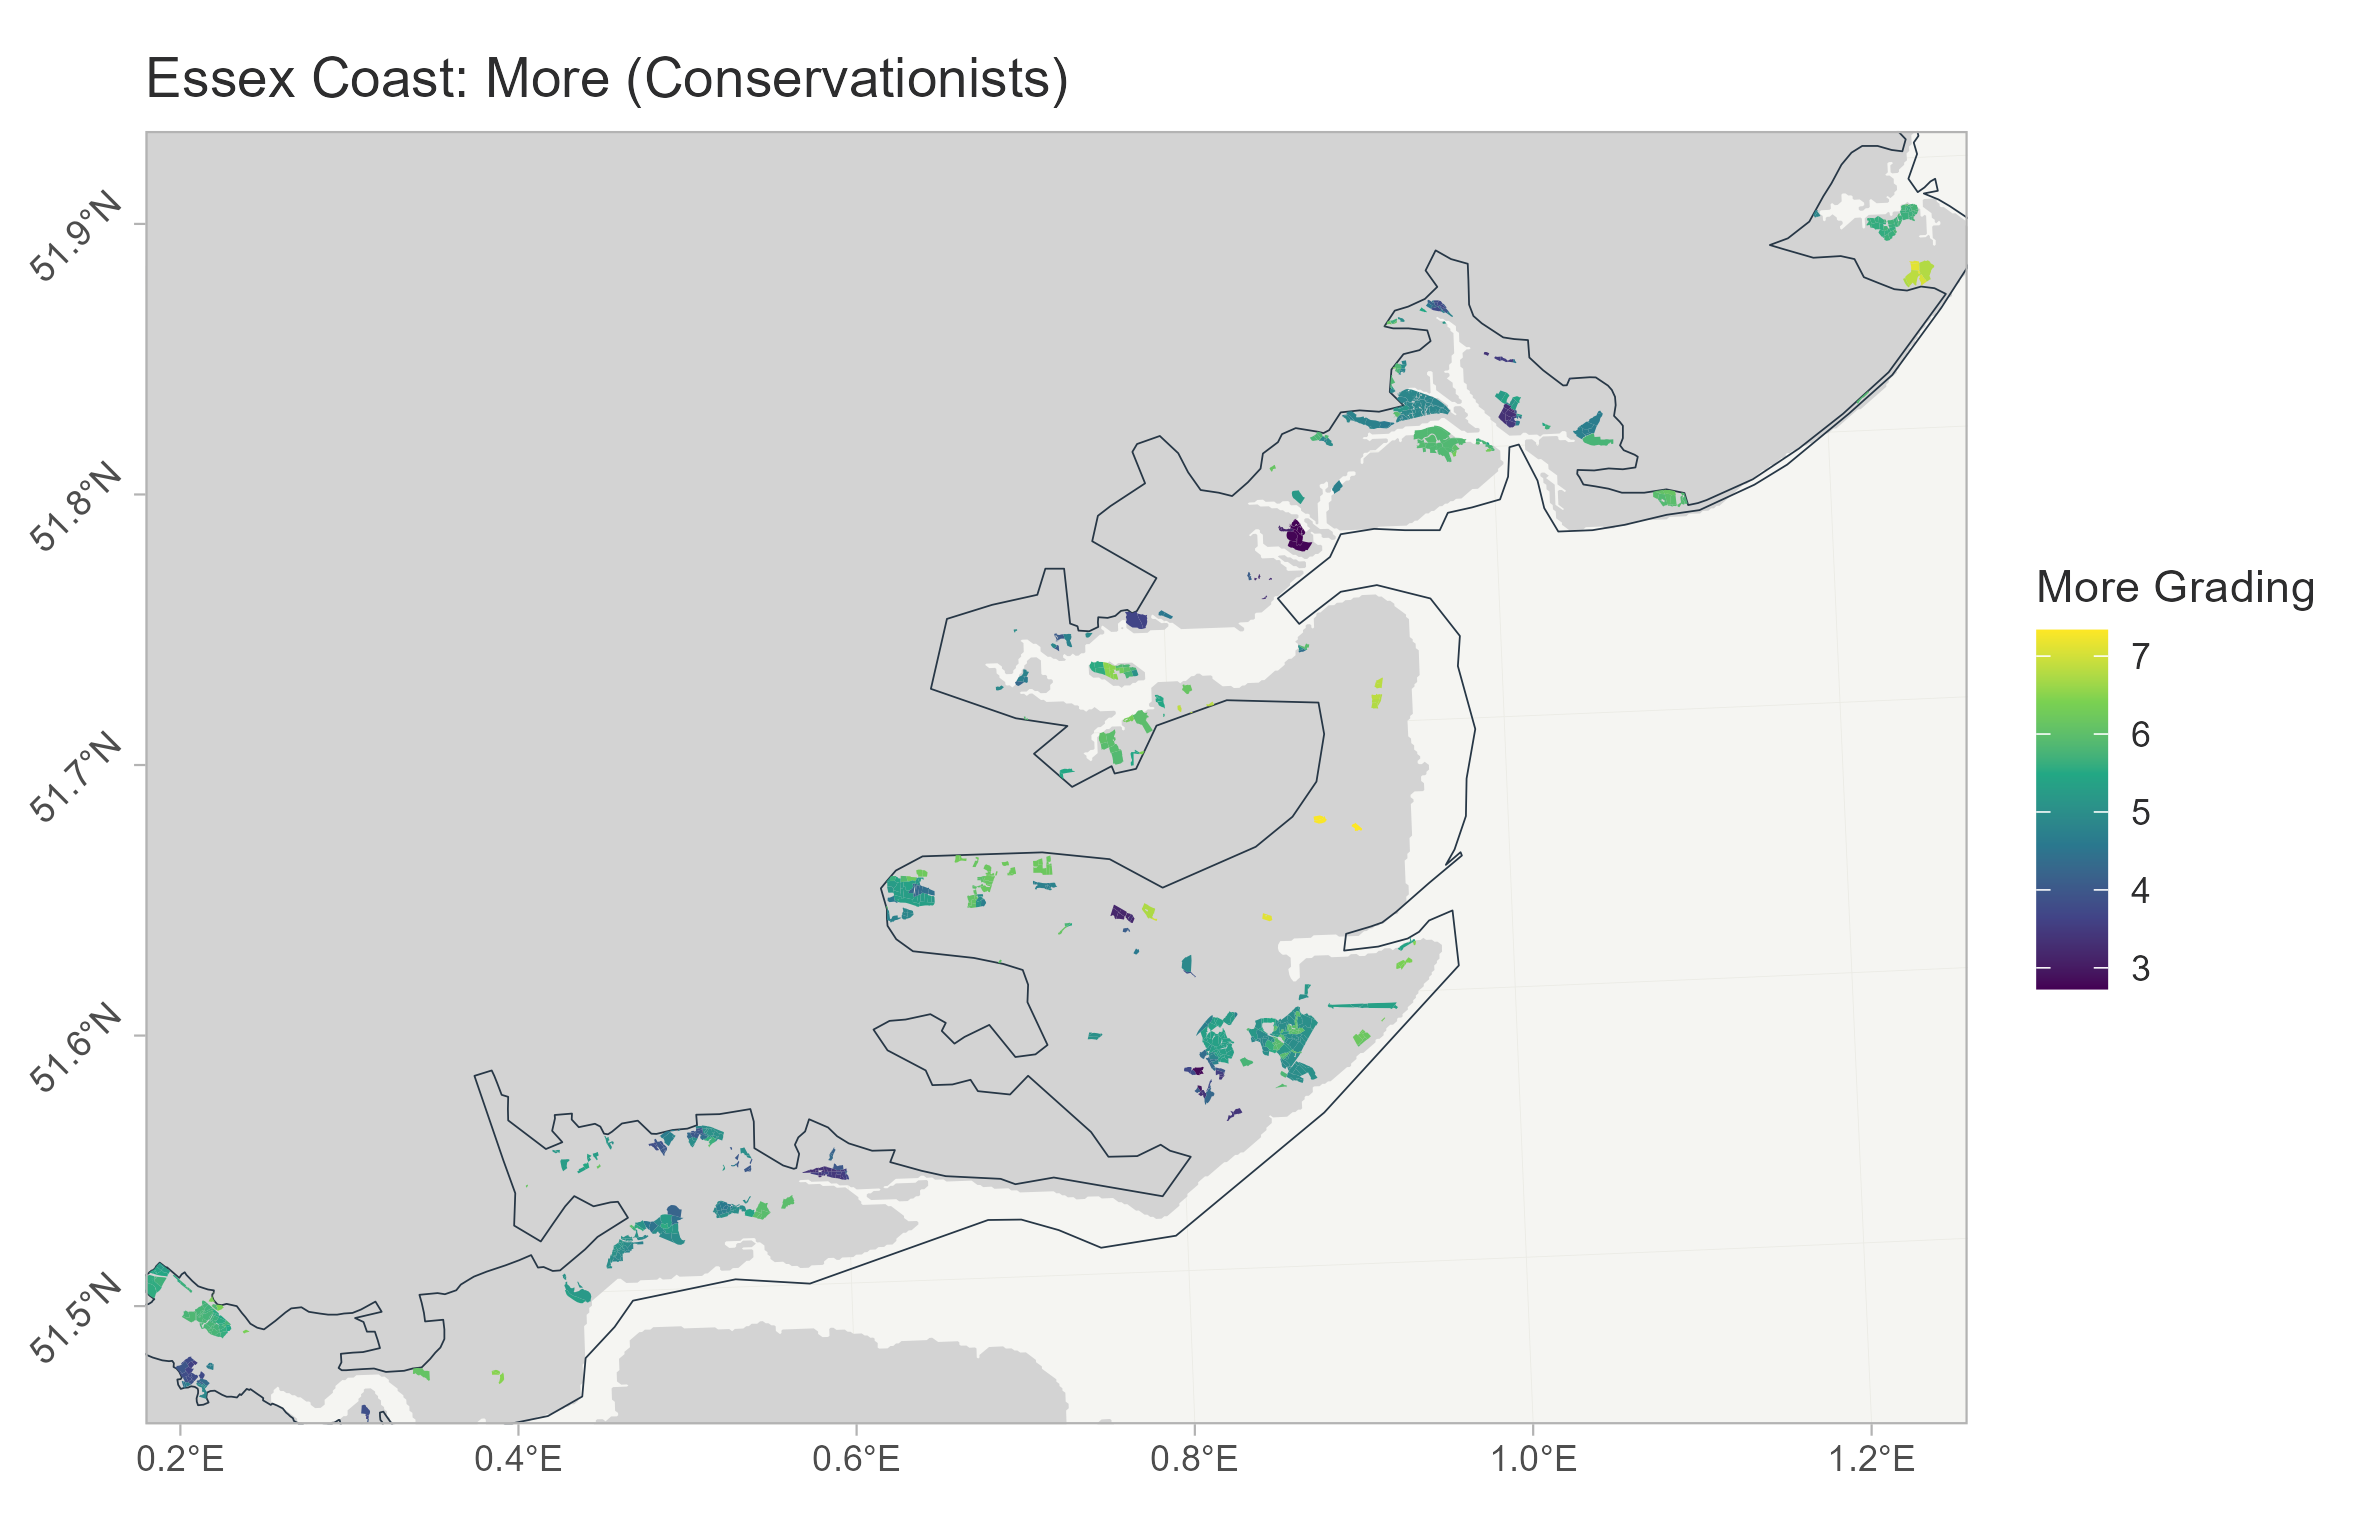
\includegraphics[width=7.29167in,height=\textheight]{Plots/Essex_G1_More.png}

}

\caption{\label{fig-EsMoreG1}Stakeholder gradings for group 1 in Essex
for the more principle of nature restoration}

\end{figure}%

\begin{figure}[H]

\centering{

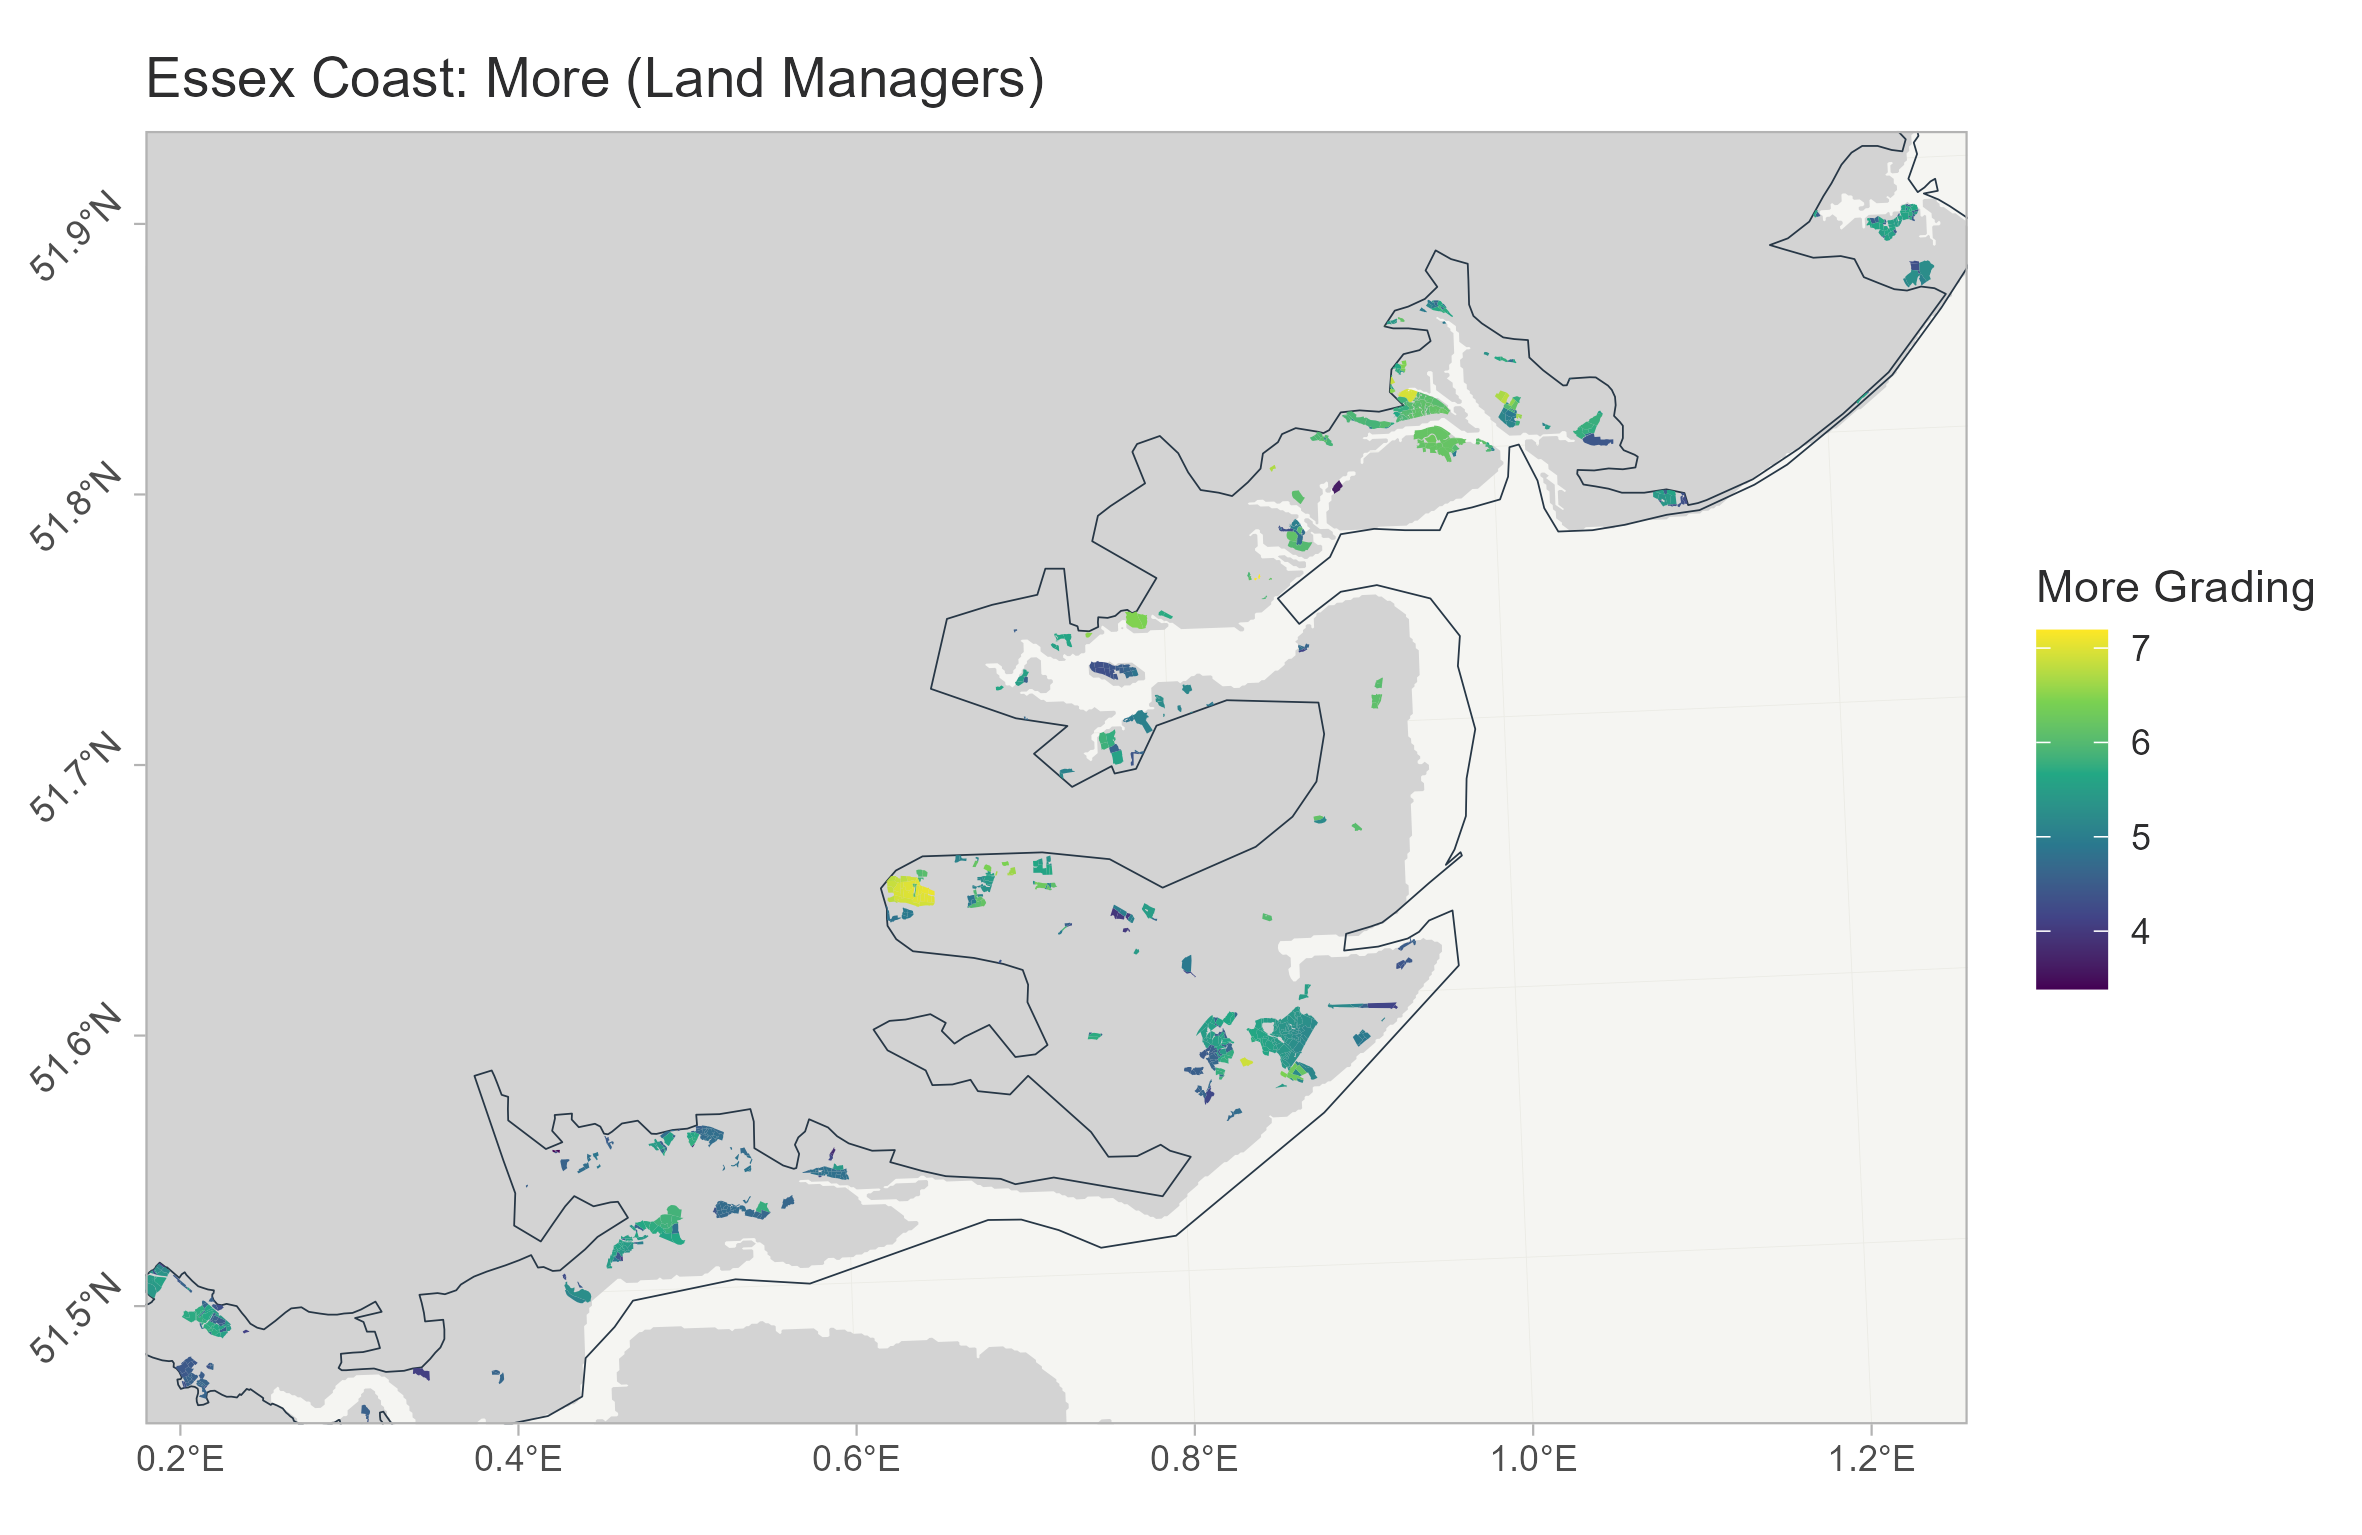
\includegraphics[width=7.29167in,height=\textheight]{Plots/Essex_G2_More.png}

}

\caption{\label{fig-EsMoreG2}Stakeholder gradings for group 2 in Essex
for the more principle of nature restoration}

\end{figure}%

\newpage{}

\paragraph{Essex: Arable Conversion for
Bigger}\label{essex-arable-conversion-for-bigger}

The stakeholder preferences for the conversion of arable land to lowland
wet grassland under the bigger principle of nature restoration for group
1 (Figure~\ref{fig-EsArBigG1}) and 2 (Figure~\ref{fig-EsArBigG2}).

\begin{figure}[H]

\centering{

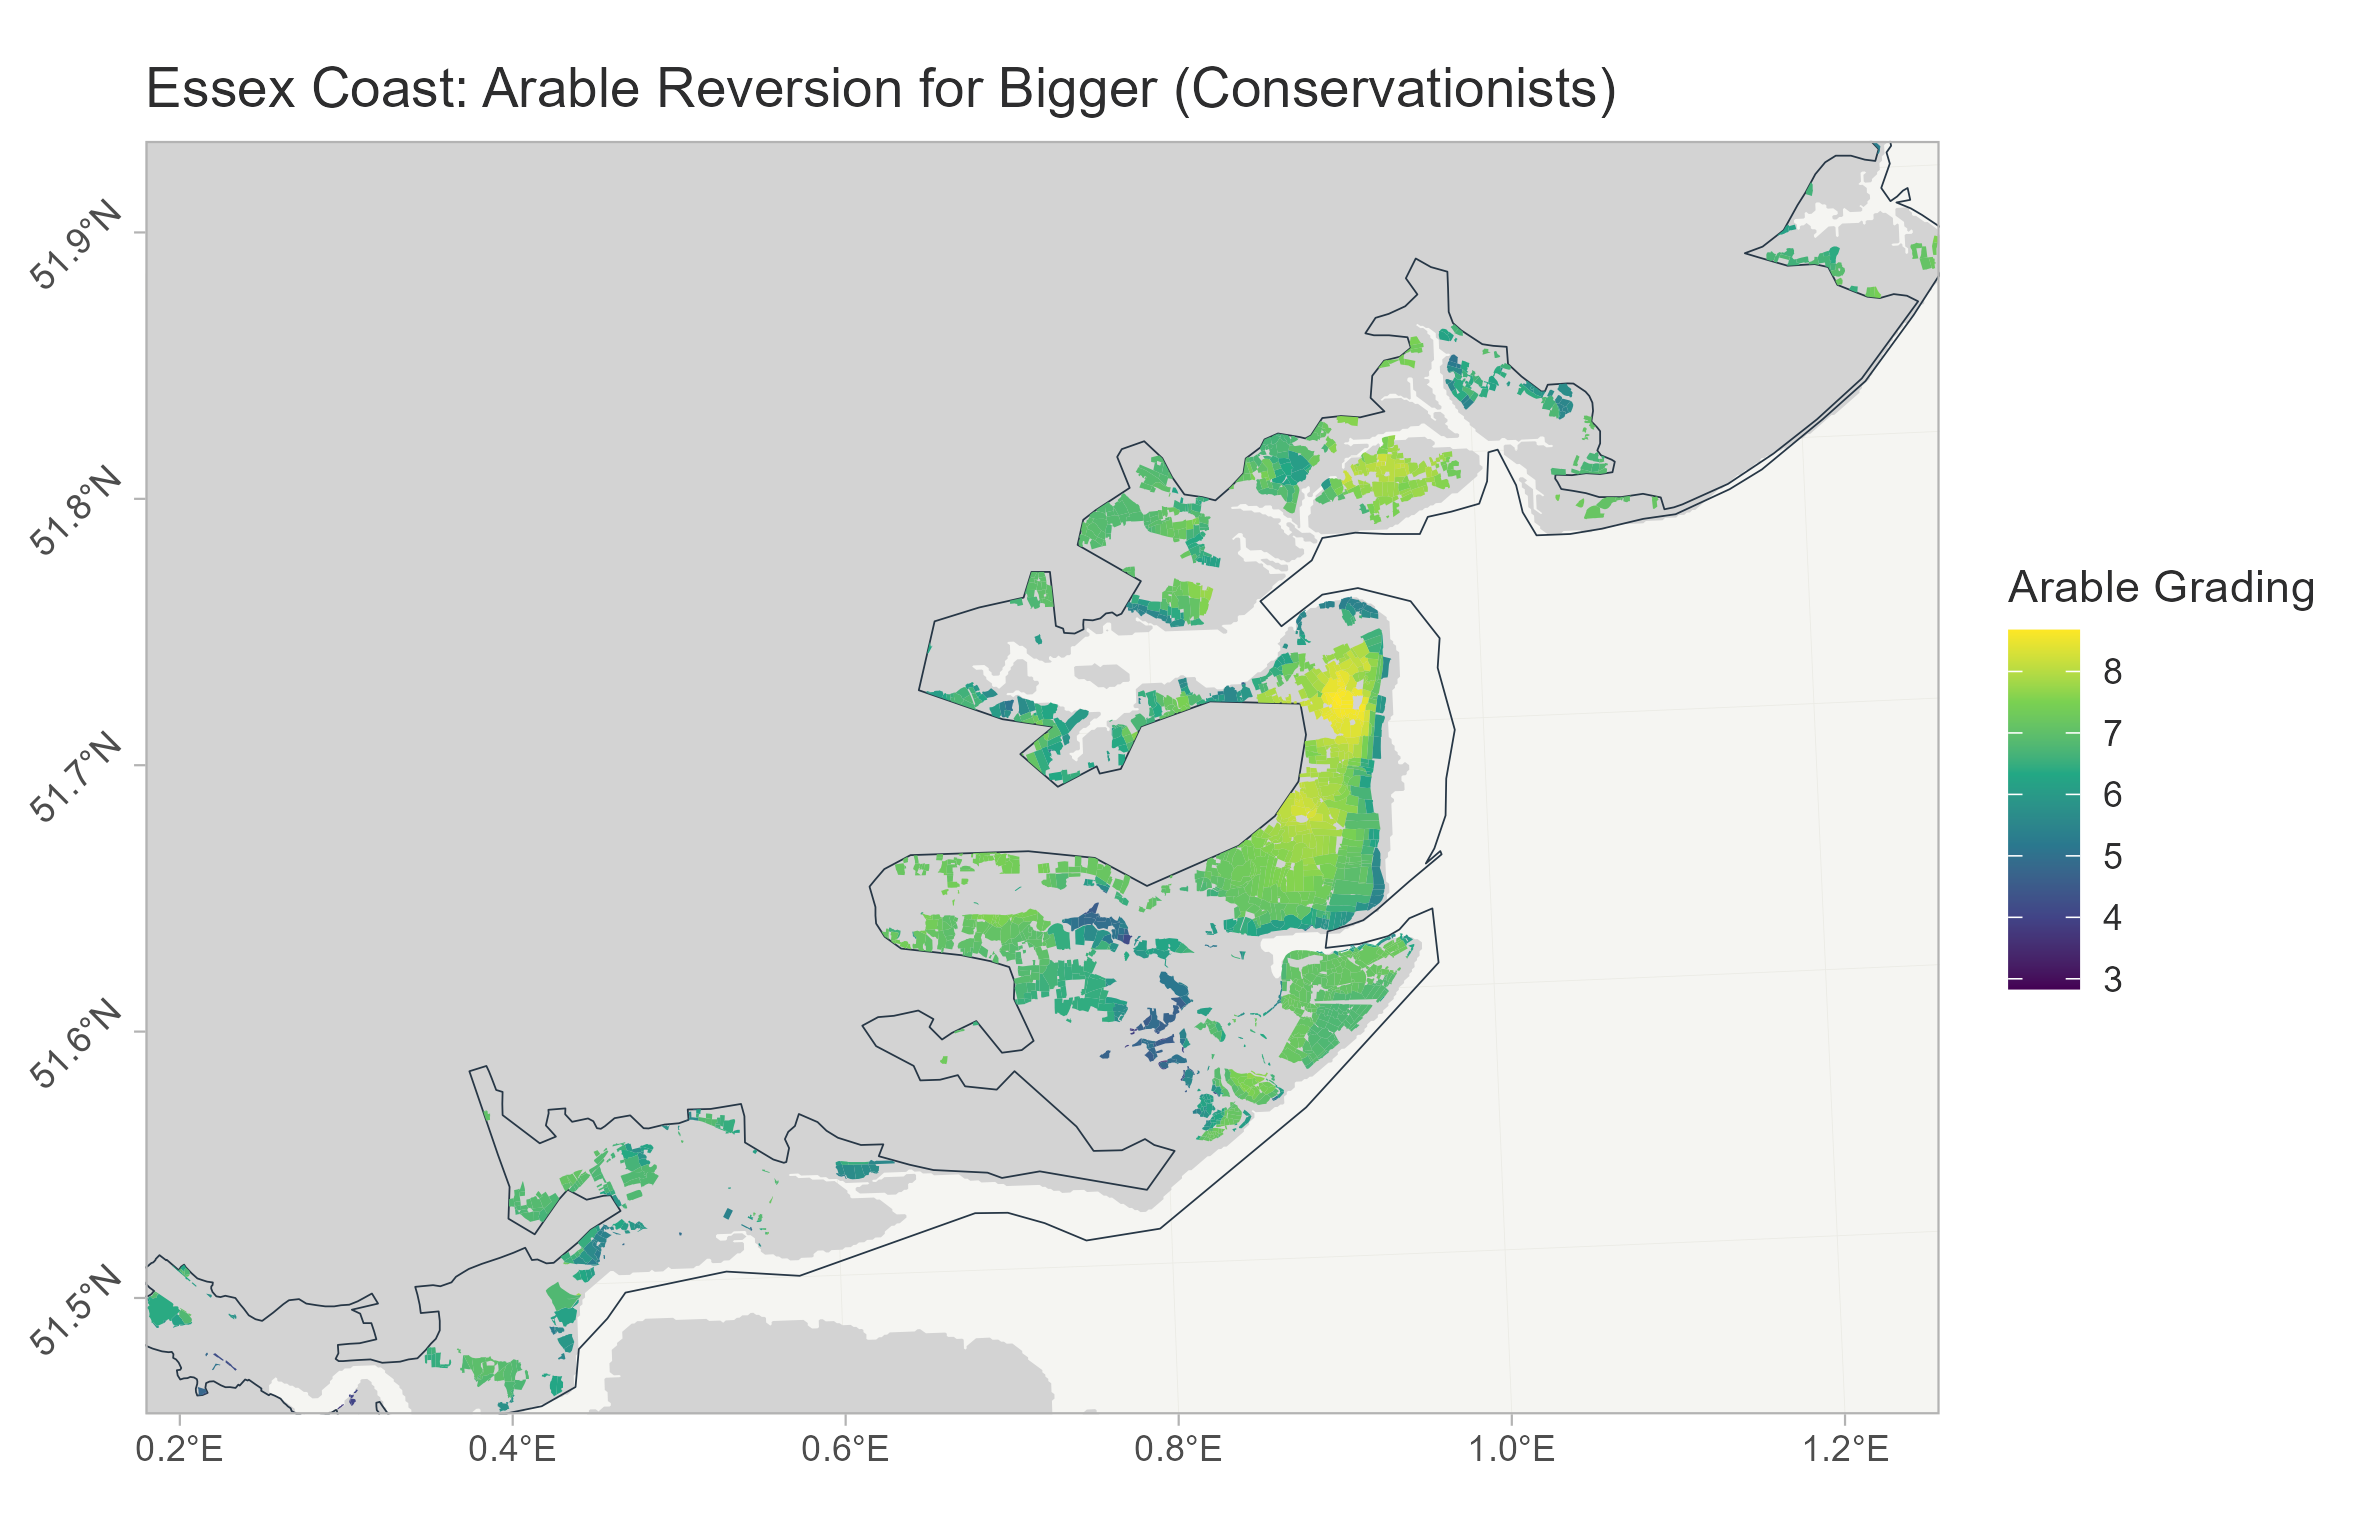
\includegraphics[width=7.29167in,height=\textheight]{Plots/Essex_G1_ArableBig.png}

}

\caption{\label{fig-EsArBigG1}Stakeholder gradings for group 1 in Essex
for the reversion of arable land to lowland wet grassland under the
bigger principle of nature restoration}

\end{figure}%

\begin{figure}[H]

\centering{

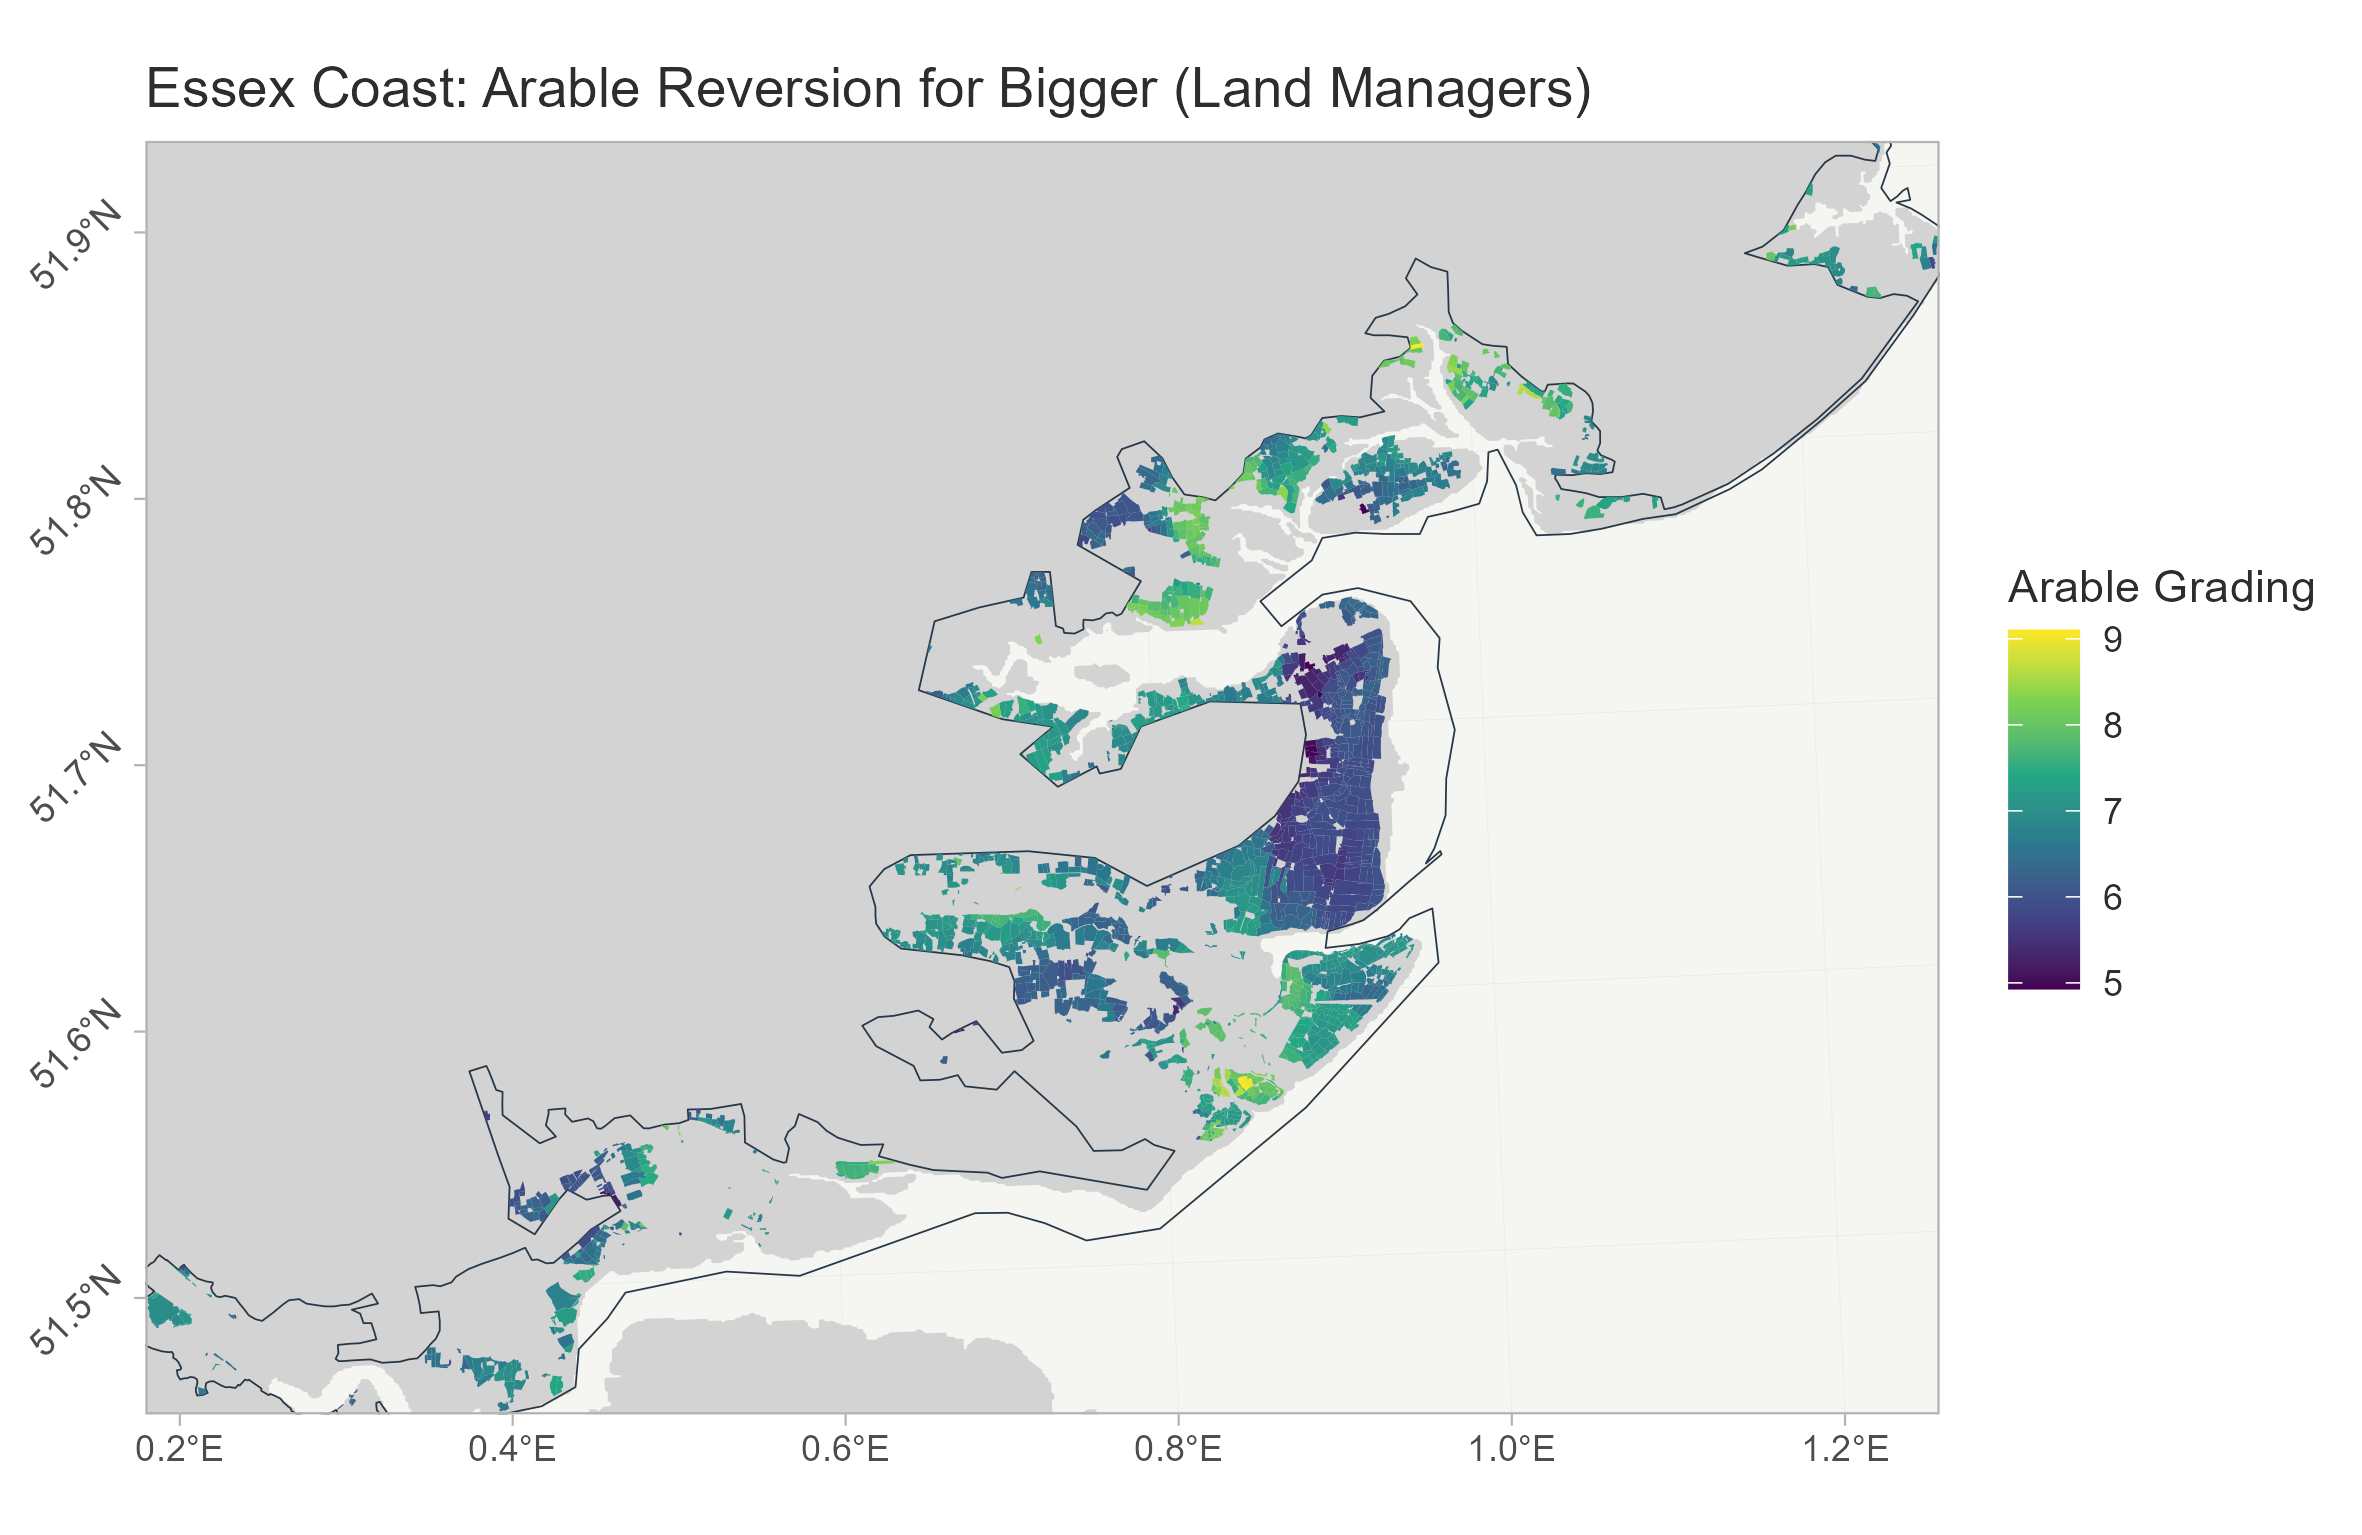
\includegraphics[width=7.29167in,height=\textheight]{Plots/Essex_G2_ArableBig.png}

}

\caption{\label{fig-EsArBigG2}Stakeholder gradings for group 2 in Essex
for the reversion of arable land to lowland wet grassland under the
bigger principle of nature restoration}

\end{figure}%

\newpage{}

\paragraph{Essex: Arable Conversion for
More}\label{essex-arable-conversion-for-more}

The stakeholder preferences for the conversion of arable land to lowland
wet grassland under the more principle of nature restoration for group 1
(Figure~\ref{fig-EsArMoreG1}) and 2 (Figure~\ref{fig-EsArMoreG2}).

\begin{figure}[H]

\centering{

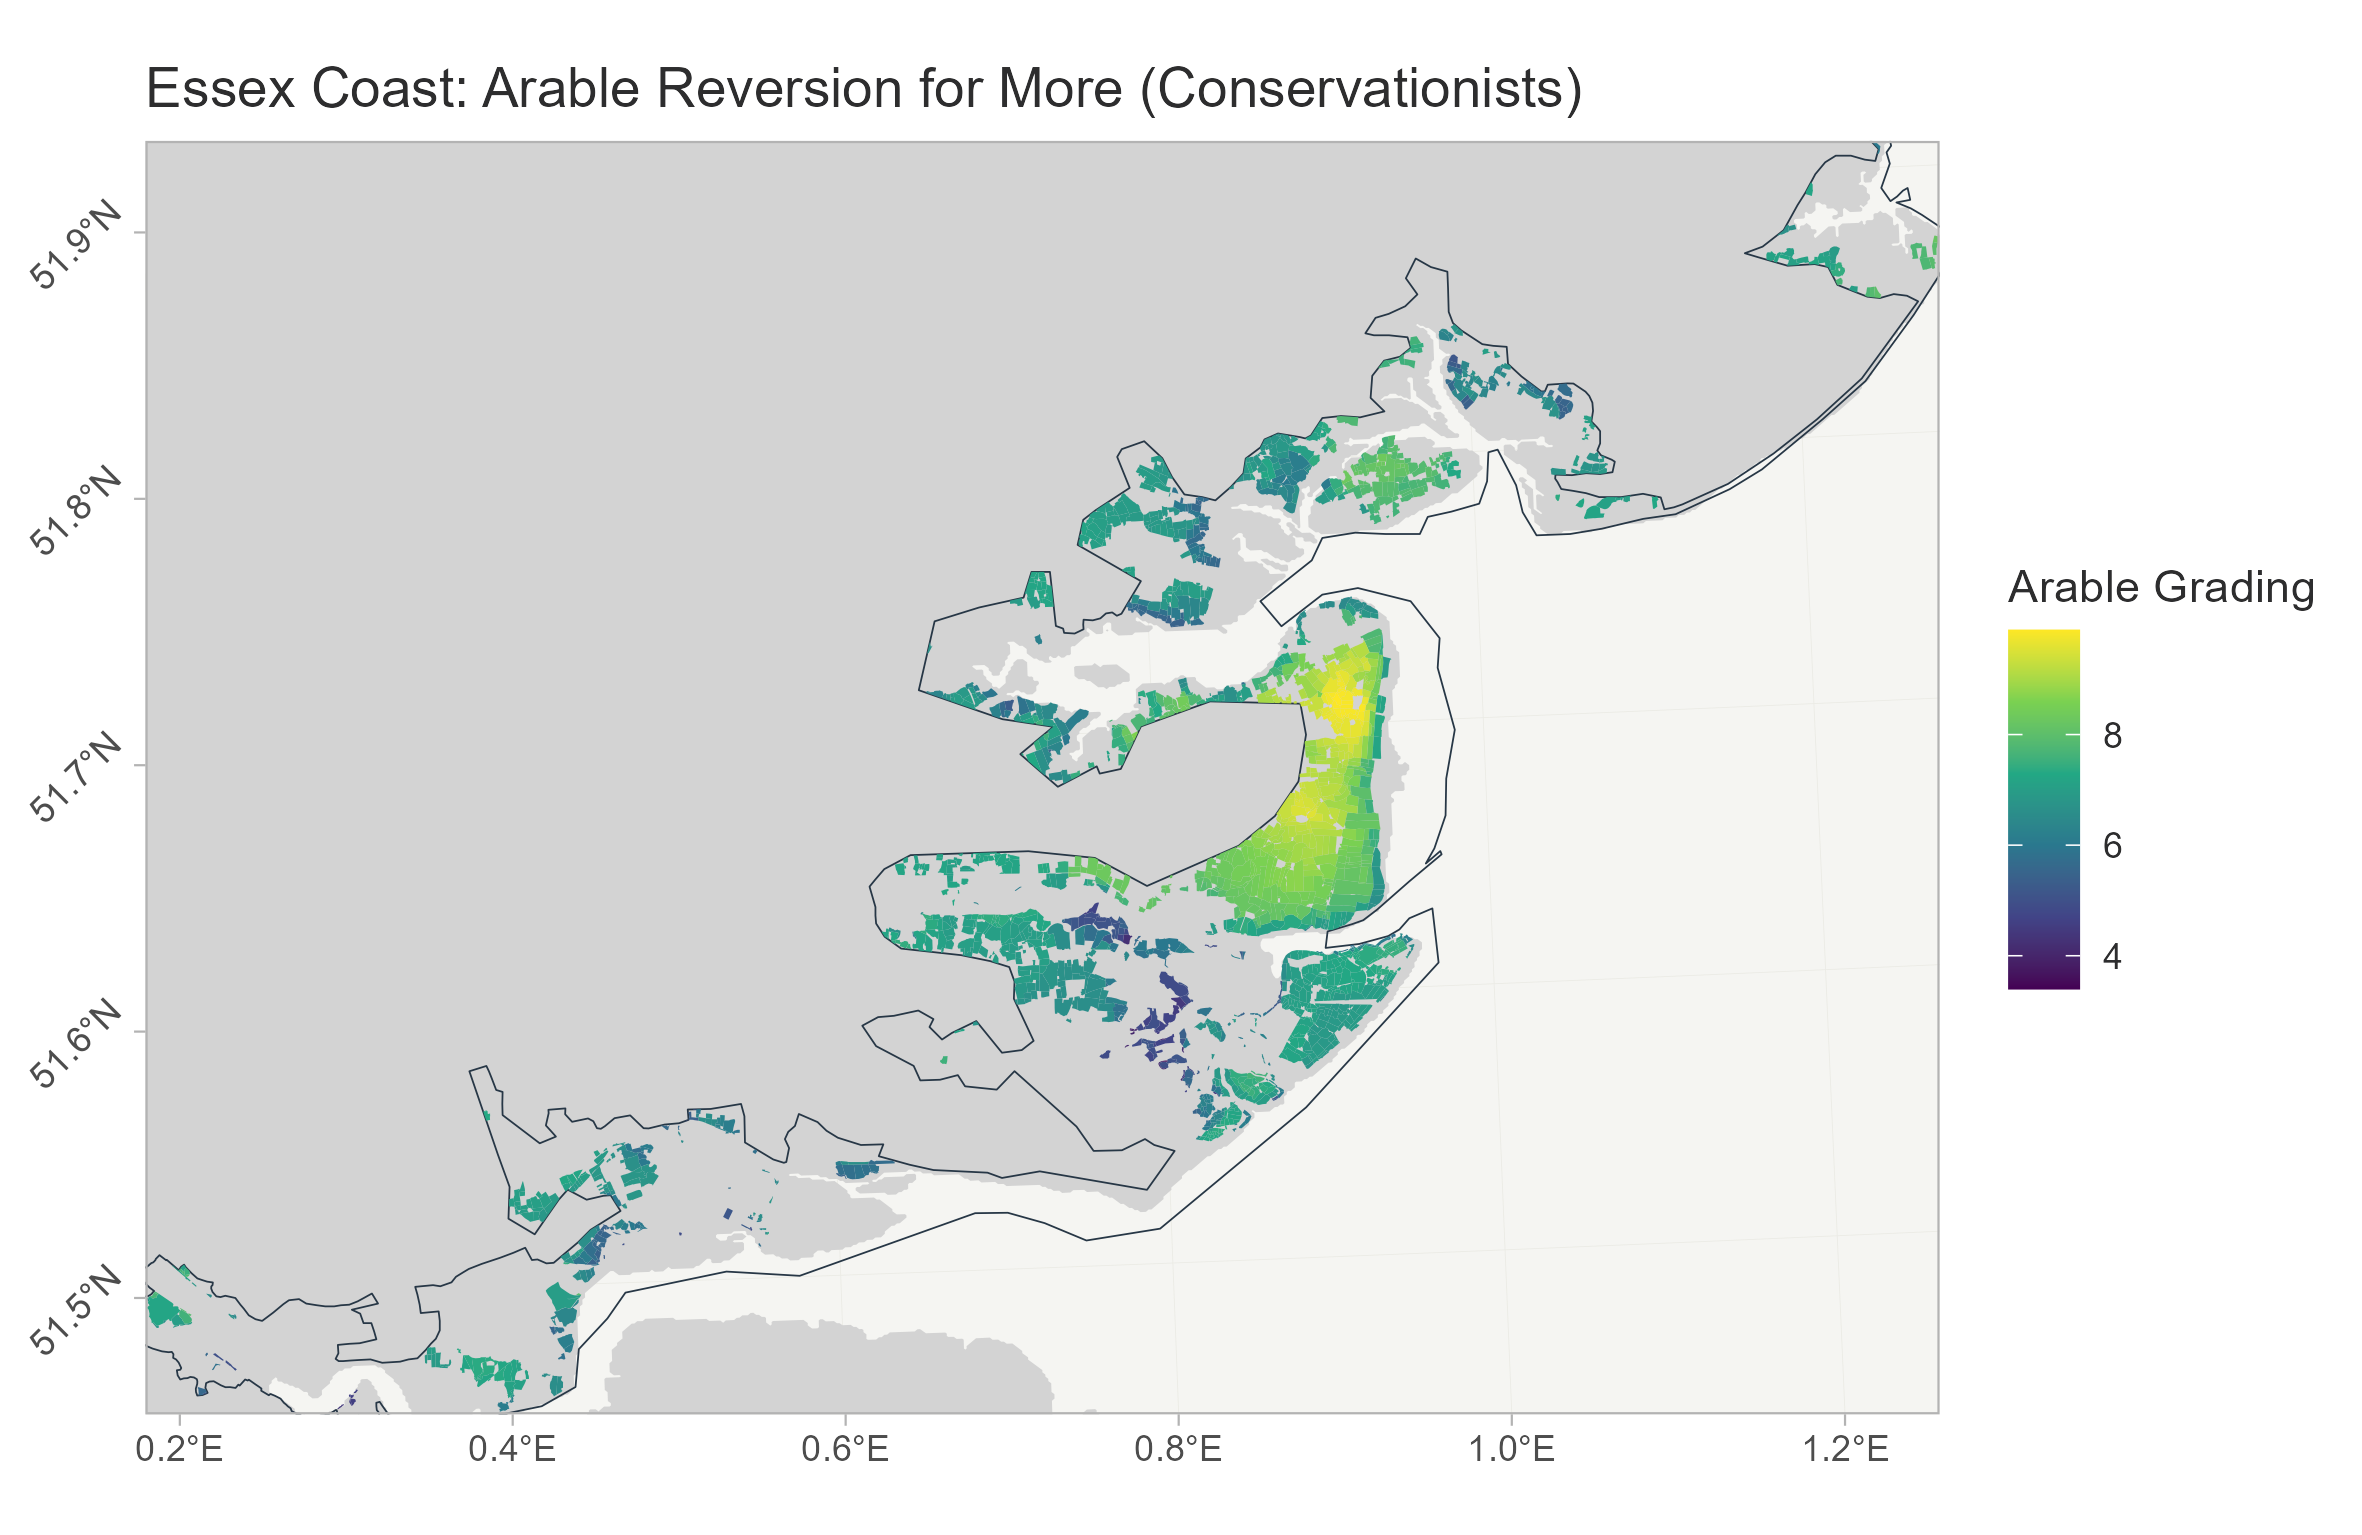
\includegraphics[width=7.29167in,height=\textheight]{Plots/Essex_G1_ArableMore.png}

}

\caption{\label{fig-EsArMoreG1}Stakeholder gradings for group 1 in Essex
for the reversion of arable land to lowland wet grassland under the more
principle of nature restoration}

\end{figure}%

\begin{figure}[H]

\centering{

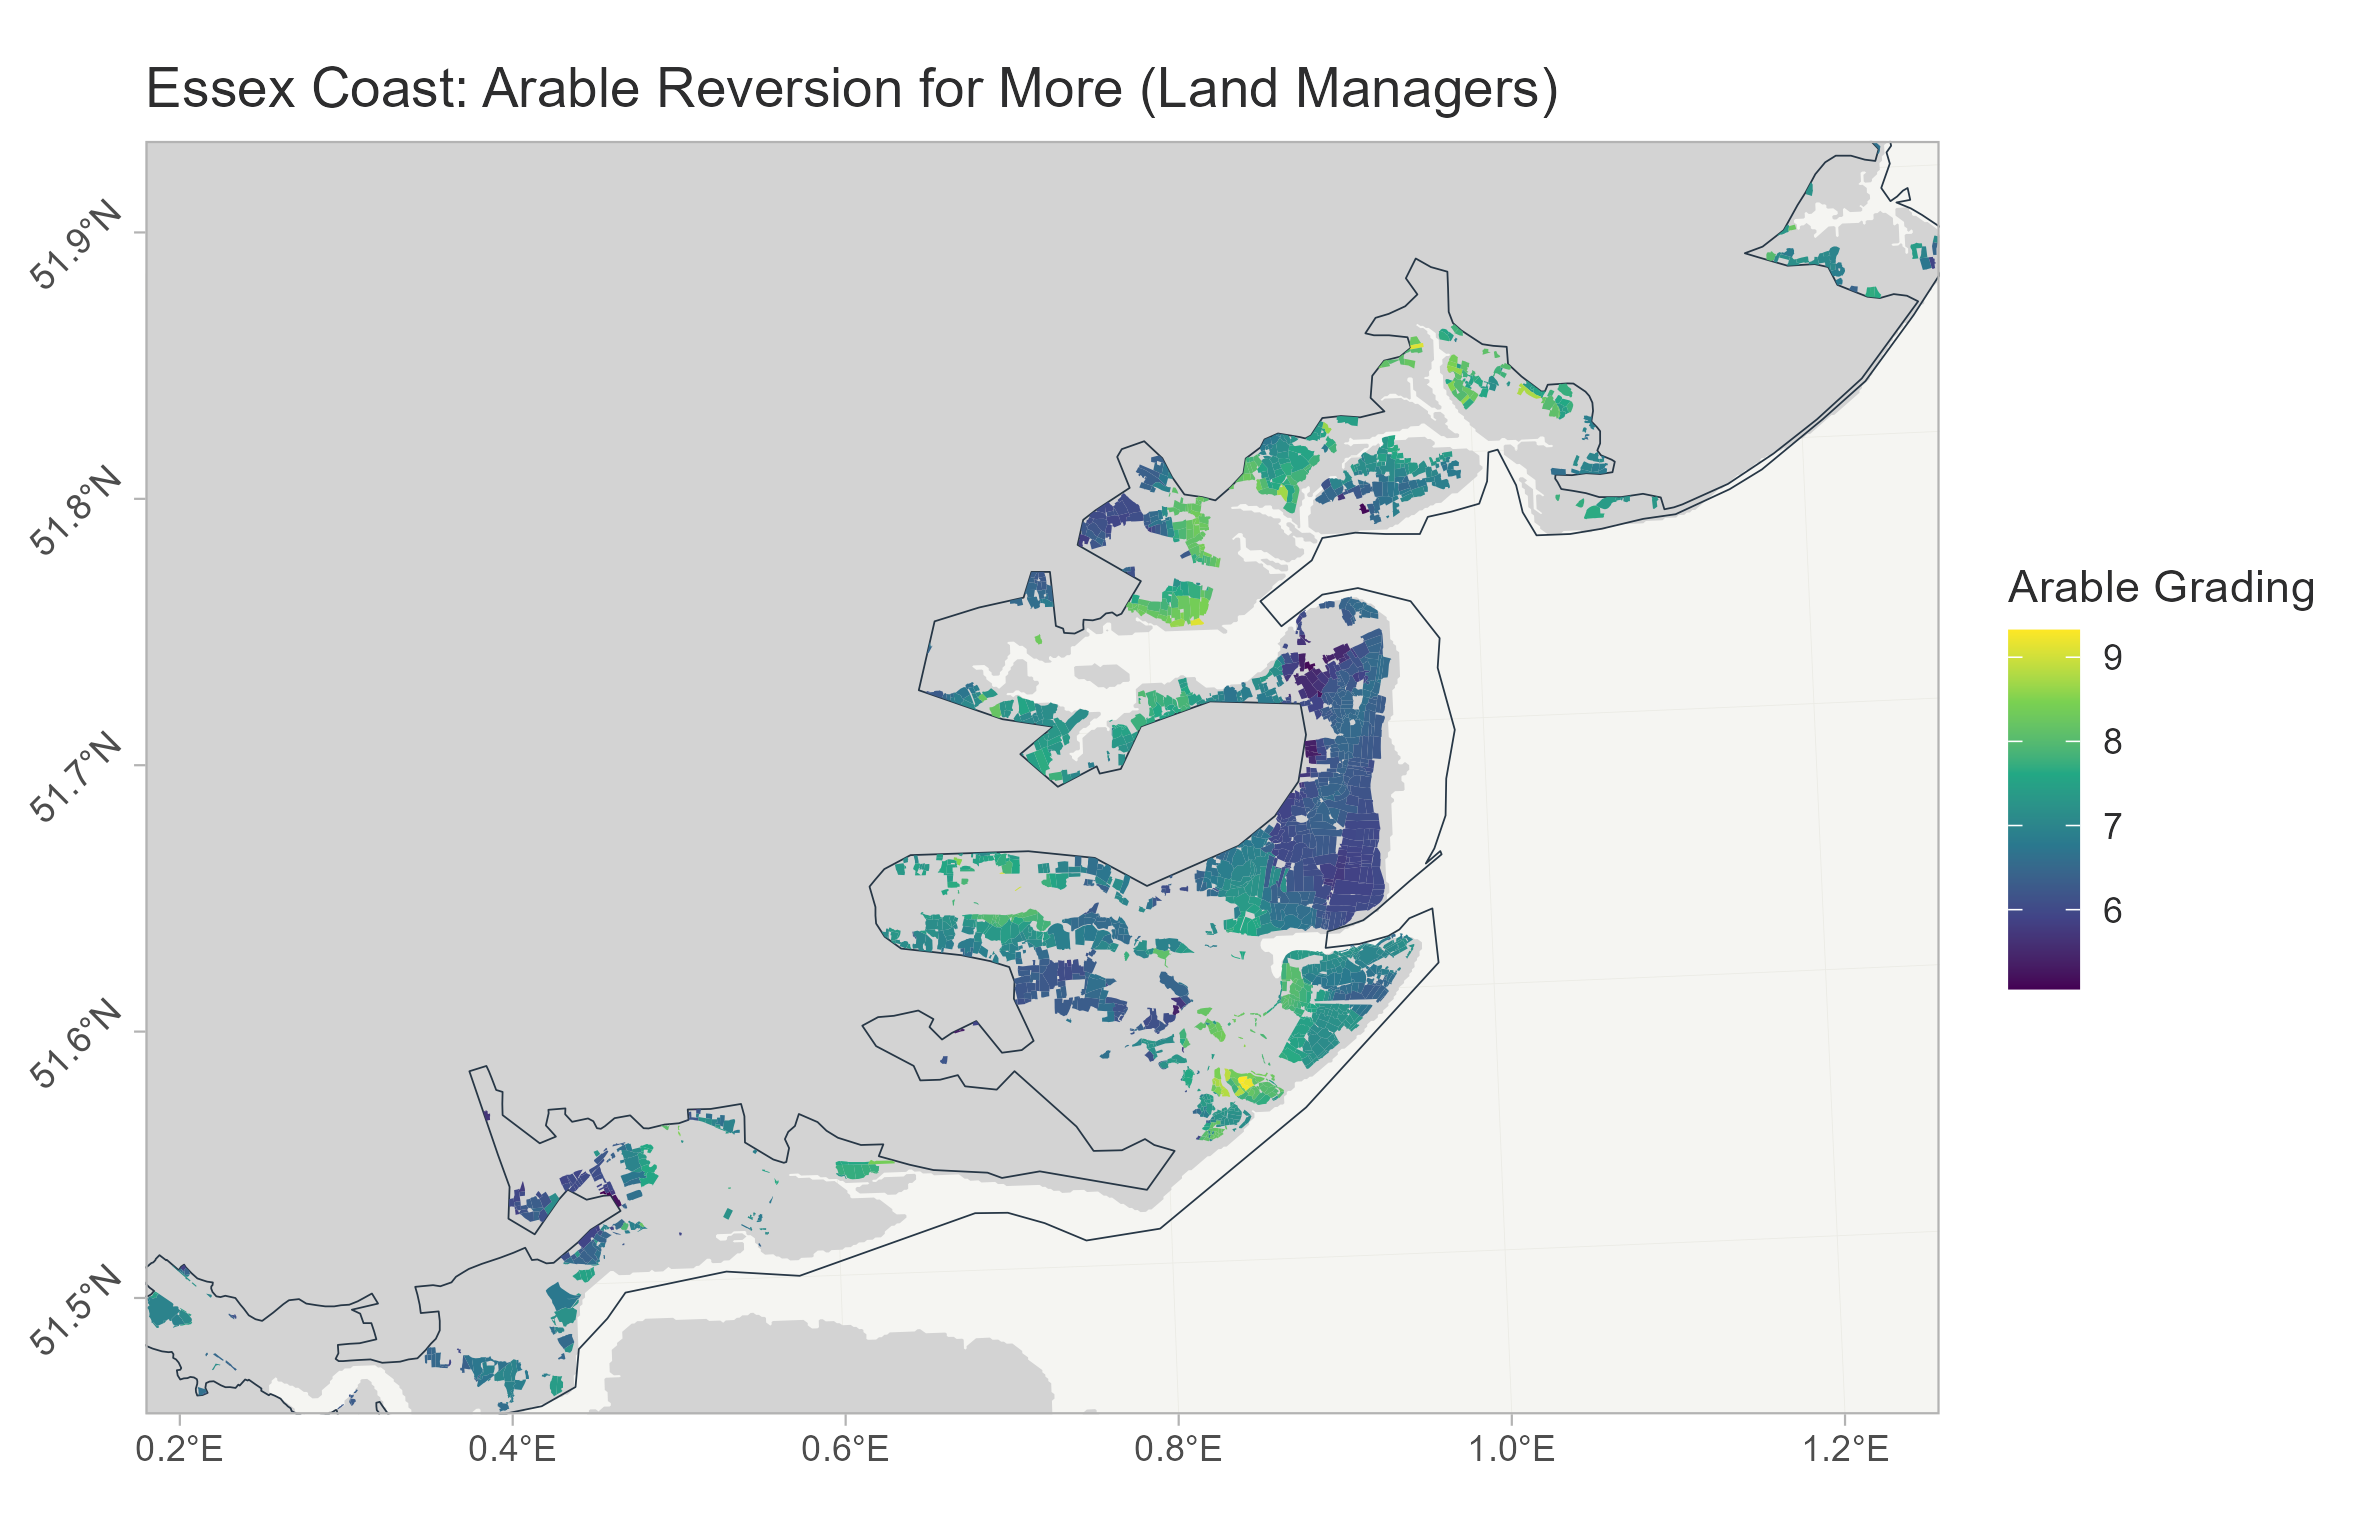
\includegraphics[width=7.29167in,height=\textheight]{Plots/Essex_G2_ArableMore.png}

}

\caption{\label{fig-EsArMoreG2}Stakeholder gradings for group 2 in Essex
for the reversion of arable land to lowland wet grassland under the more
principle of nature restoration}

\end{figure}%

\newpage{}

\subsubsection{Somerset Levels Results}\label{somerset-levels-results}

For the Somerset Levels we had three different stakeholder groups. Group
1 (G1) was a group of conservationists, group 2 was a group of various
body representatives tasked with wider objectives than the preservation
of biodiversity (e.g.~Natural England, Internal drainage board,
Environment Agency and South West FWAG) group 3 was a group of
landowners and farmers.

\paragraph{Somerset Levels: Better}\label{somerset-levels-better}

The stakeholder preferences for the better principle of nature
restoration for group 1, group 2 and group 3 can be visualized in
(Figure~\ref{fig-SomBetterG1}), (Figure~\ref{fig-SomBetterG2}) and
(Figure~\ref{fig-SomBetterG3}) receptively. The stakeholder guidelines
that were used to produce these maps can be found in
Table~\ref{tbl-SomG1} for group 1, Table~\ref{tbl-SomG2} for group 2 and
Table~\ref{tbl-SomG3} for group 3.

\begin{figure}[H]

\centering{

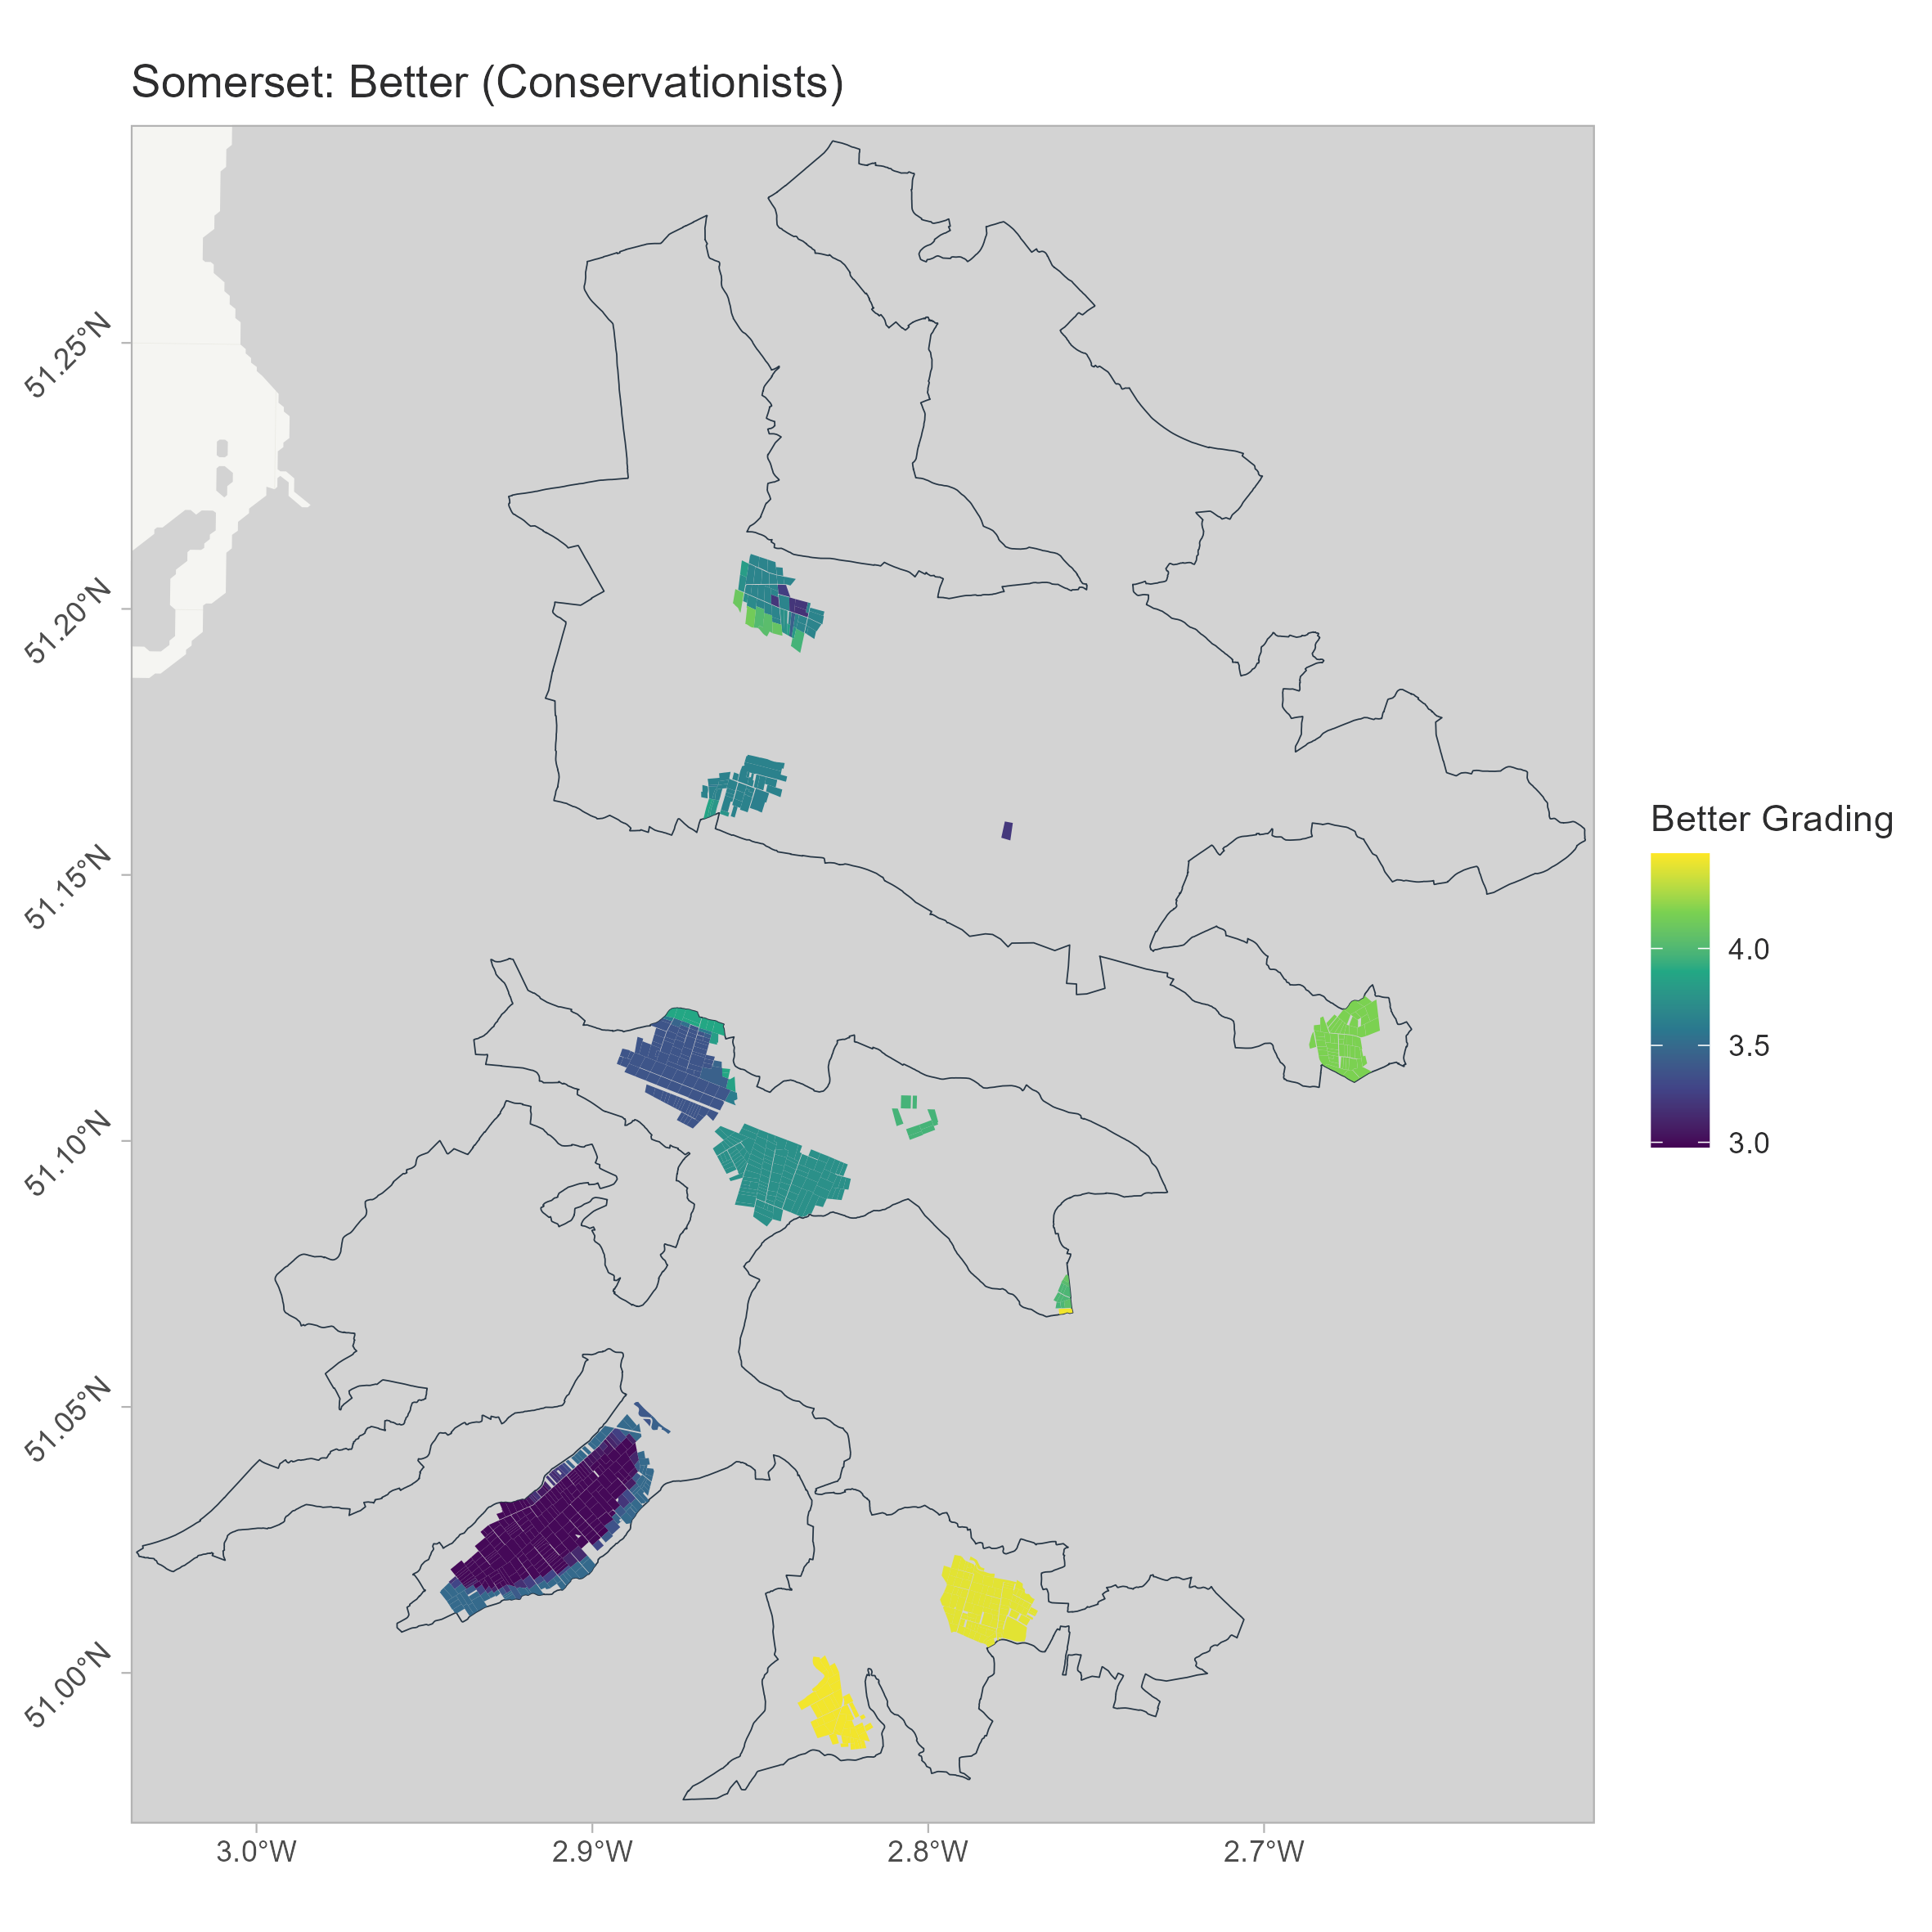
\includegraphics[width=\textwidth,height=9.375in]{Plots/Somerset_G1_Better.png}

}

\caption{\label{fig-SomBetterG1}Stakeholder gradings for group 1 in the
Somerset Levels for the better principle of nature restoration}

\end{figure}%

\begin{figure}[H]

\centering{

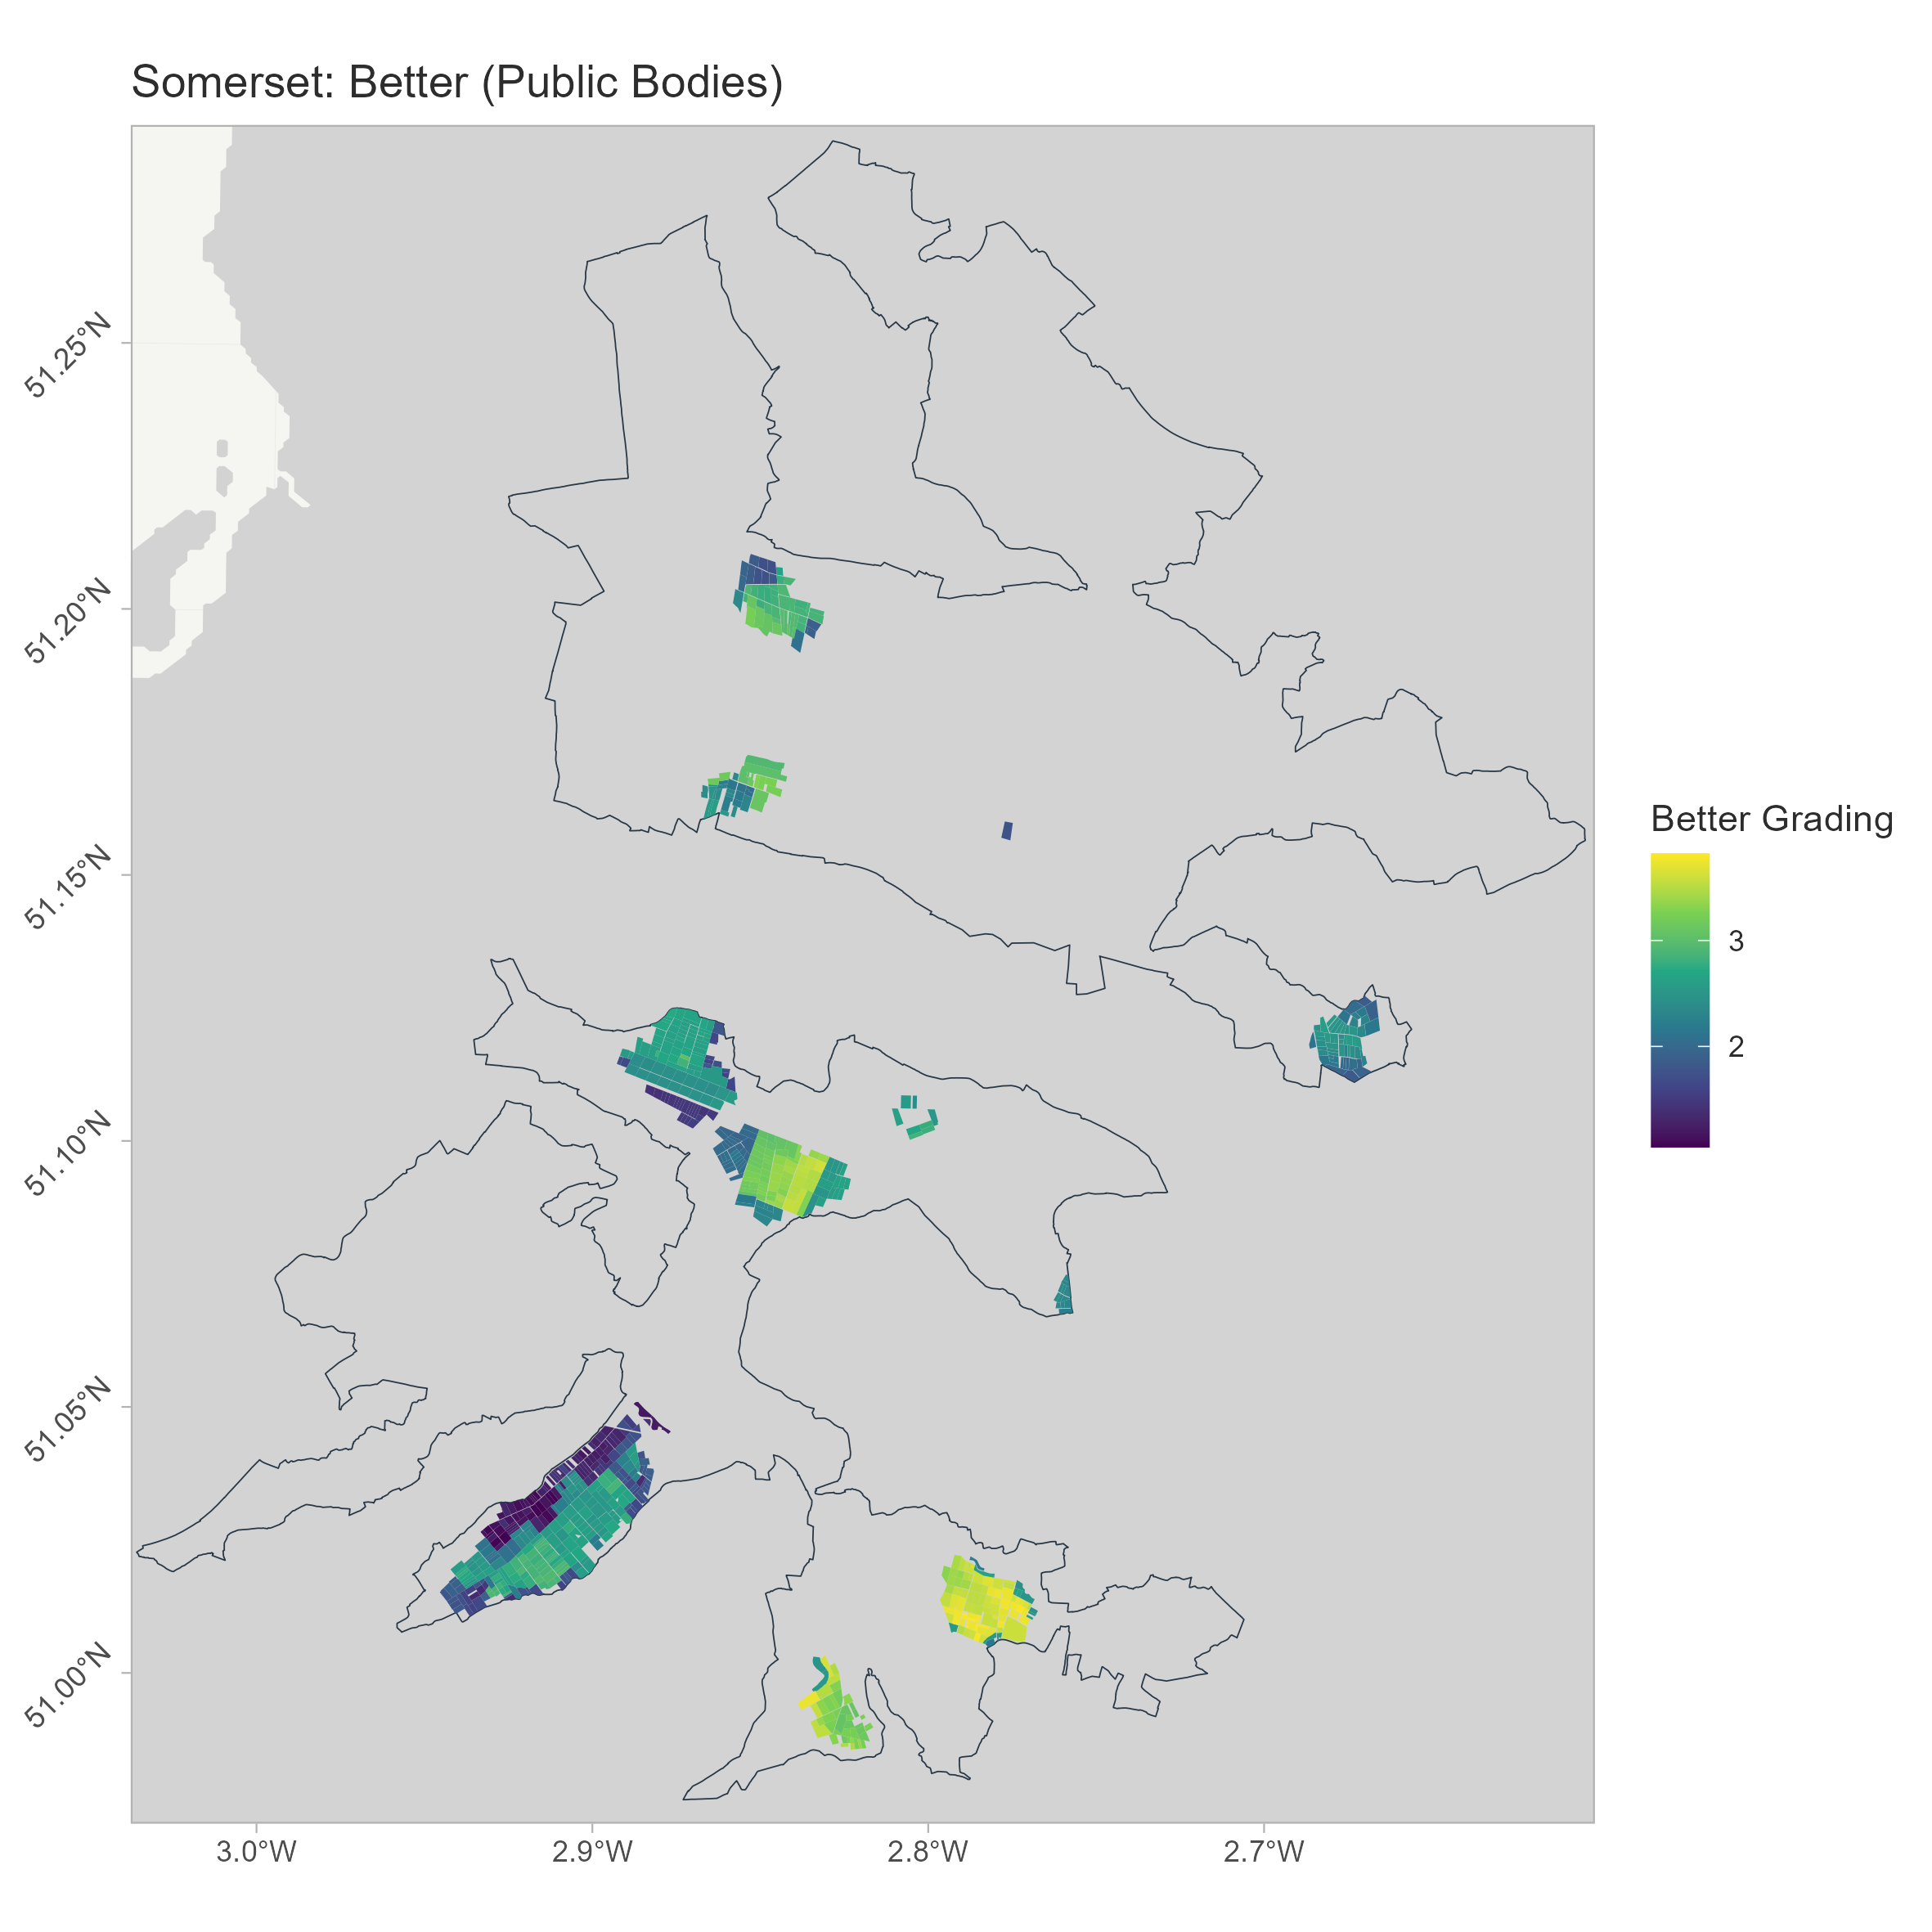
\includegraphics[width=\textwidth,height=9.375in]{Plots/Somerset_G2_Better.png}

}

\caption{\label{fig-SomBetterG2}Stakeholder gradings for group 2 in the
Somerset Levels for the better principle of nature restoration}

\end{figure}%

\begin{figure}[H]

\centering{

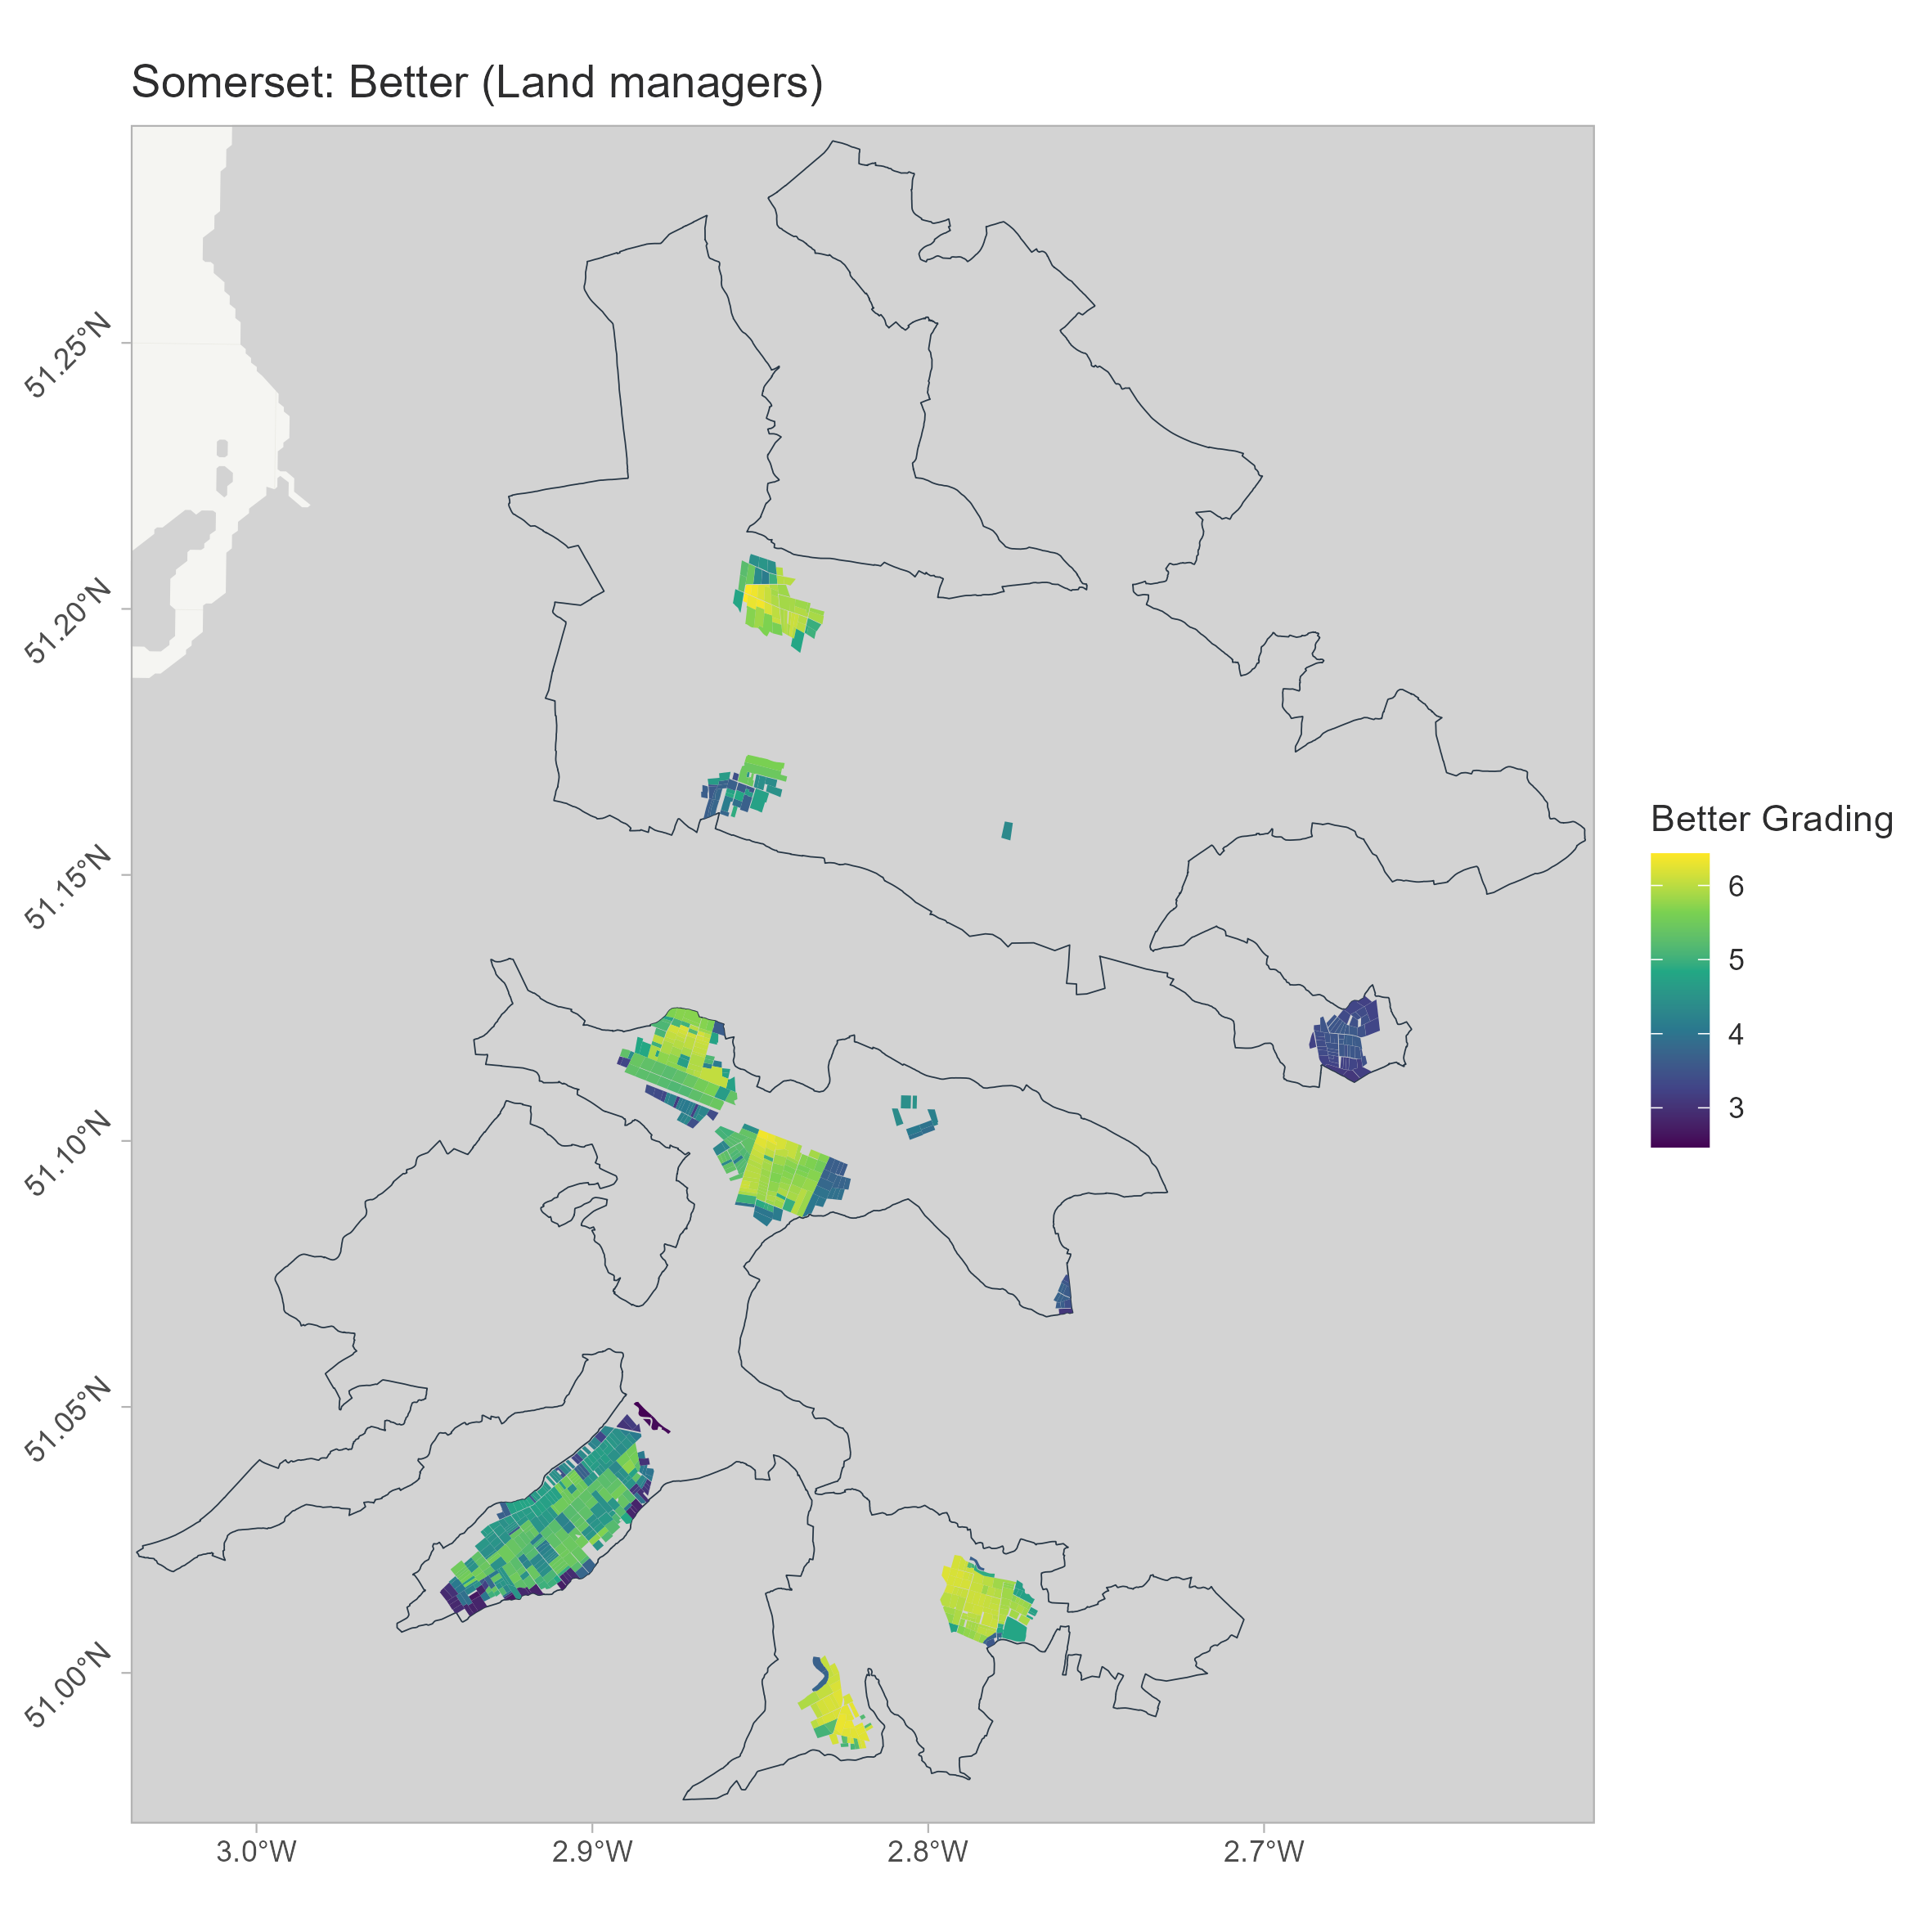
\includegraphics[width=\textwidth,height=9.375in]{Plots/Somerset_G3_Better.png}

}

\caption{\label{fig-SomBetterG3}Stakeholder gradings for group 3 in the
Somerset Levels for the better principle of nature restoration}

\end{figure}%

\newpage{}

\paragraph{Somerset Levels: Bigger}\label{somerset-levels-bigger}

The stakeholder preferences for the bigger principle of nature
restoration for group 1 (Figure~\ref{fig-SomBigG1}), group 2
(Figure~\ref{fig-SomBigG2}) and group 3 (Figure~\ref{fig-SomBigG3}).

\begin{figure}[H]

\centering{

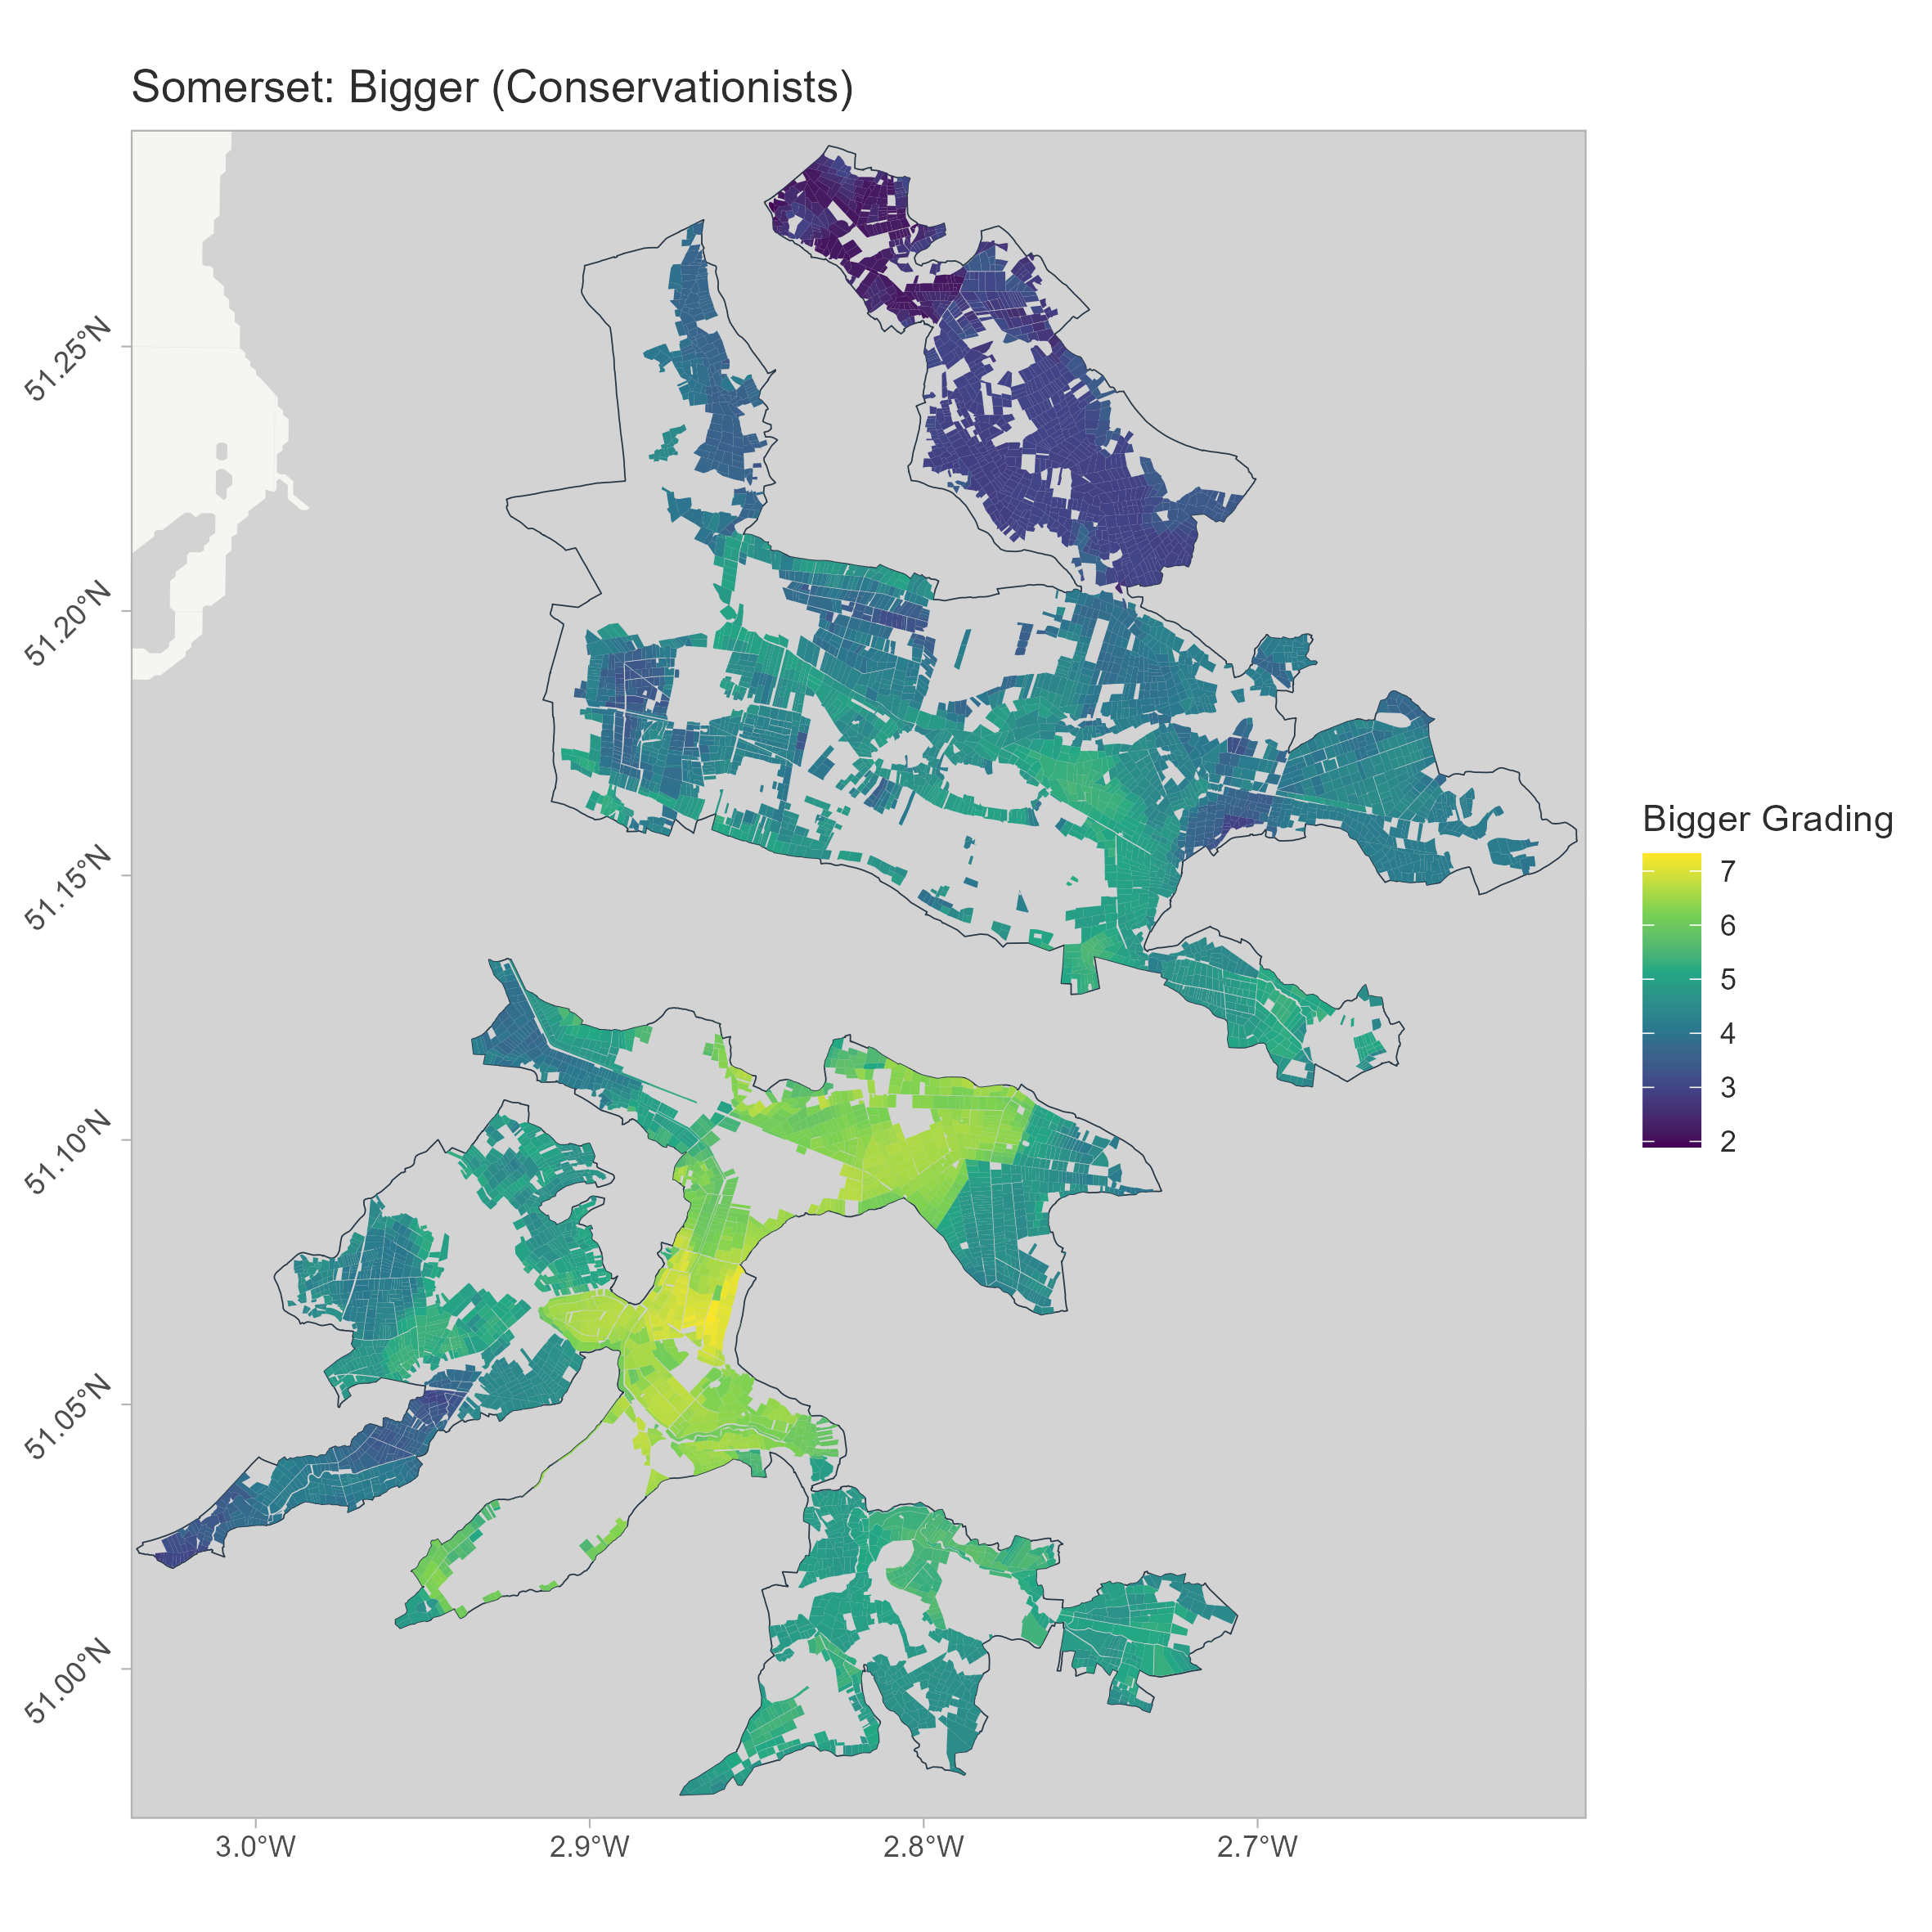
\includegraphics[width=\textwidth,height=9.375in]{Plots/Somerset_G1_Bigger.png}

}

\caption{\label{fig-SomBigG1}Stakeholder gradings for group 1 in the
Somerset Levels for the bigger principle of nature restoration}

\end{figure}%

\begin{figure}[H]

\centering{

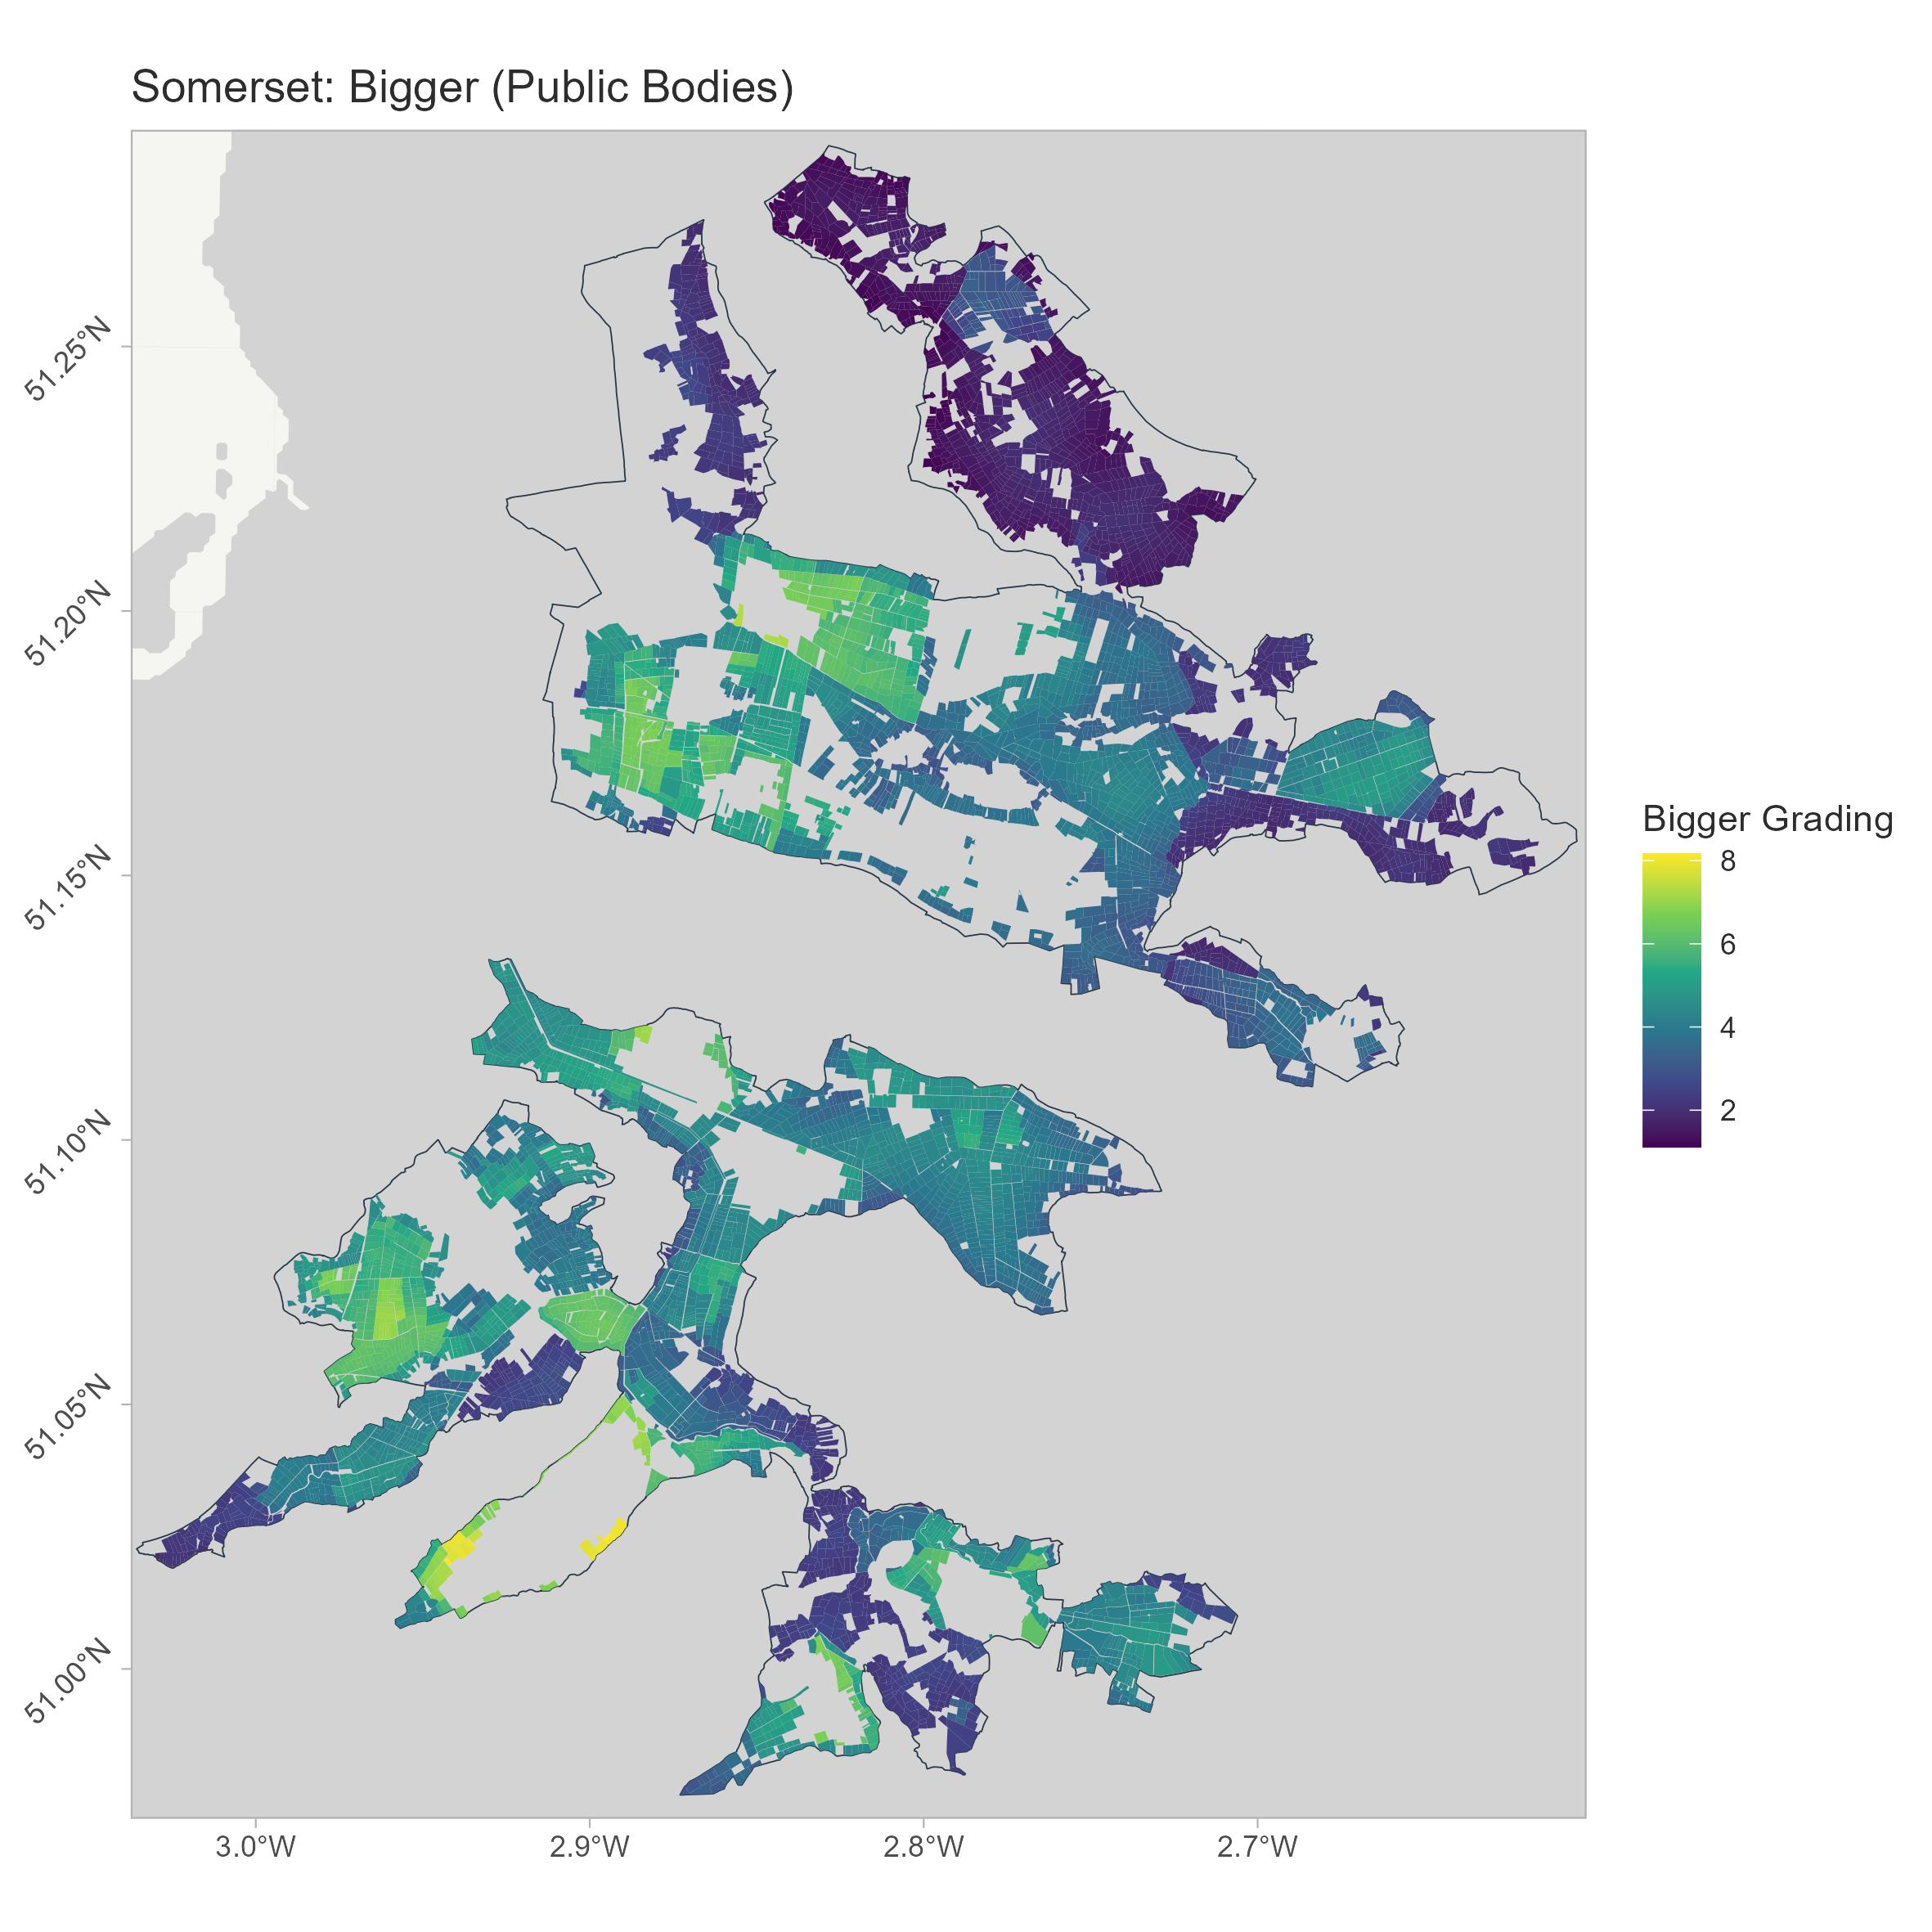
\includegraphics[width=\textwidth,height=9.375in]{Plots/Somerset_G2_Bigger.png}

}

\caption{\label{fig-SomBigG2}Stakeholder gradings for group 2 in the
Somerset Levels for the bigger principle of nature restoration}

\end{figure}%

\begin{figure}[H]

\centering{

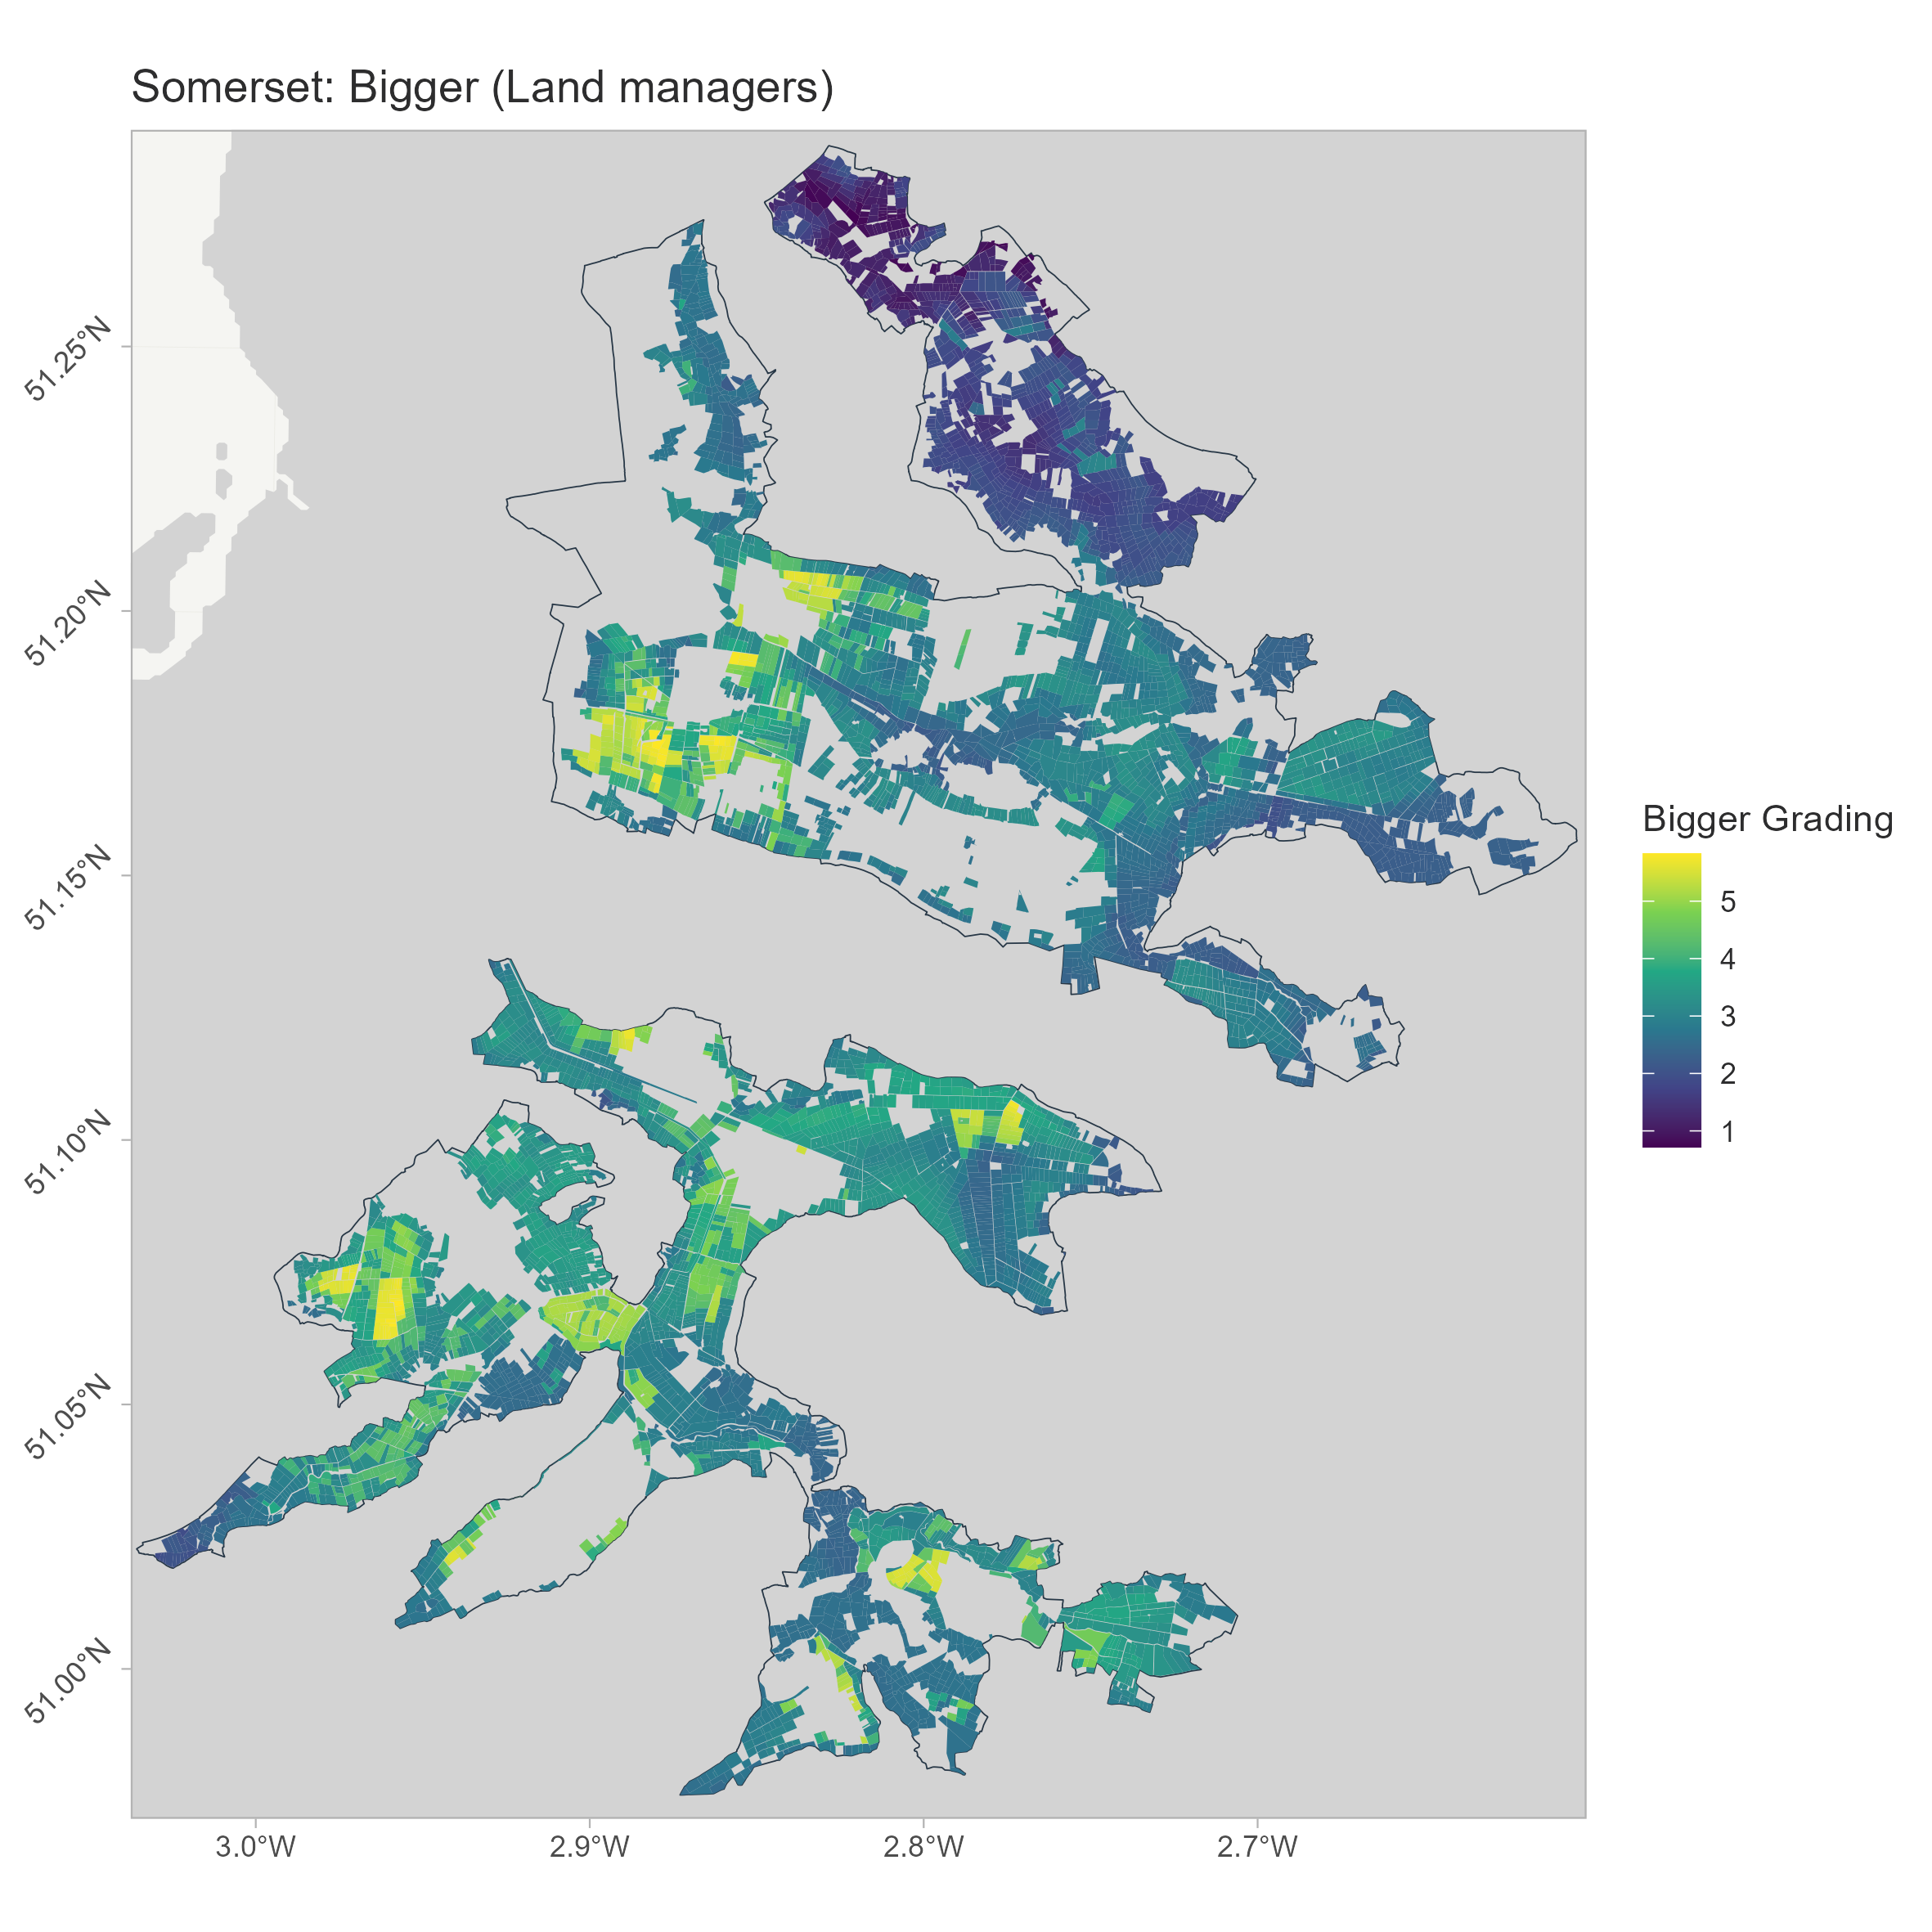
\includegraphics[width=\textwidth,height=9.375in]{Plots/Somerset_G3_Bigger.png}

}

\caption{\label{fig-SomBigG3}Stakeholder gradings for group 3 in the
Somerset Levels for the bigger principle of nature restoration}

\end{figure}%

\newpage{}

\paragraph{Somerset Levels: More}\label{somerset-levels-more}

The stakeholder preferences for the more principle of nature restoration
for group 1 (Figure~\ref{fig-SomMoreG1}), group 2
(Figure~\ref{fig-SomMoreG2}) and group 3 (Figure~\ref{fig-SomMoreG3}).

\begin{figure}[H]

\centering{

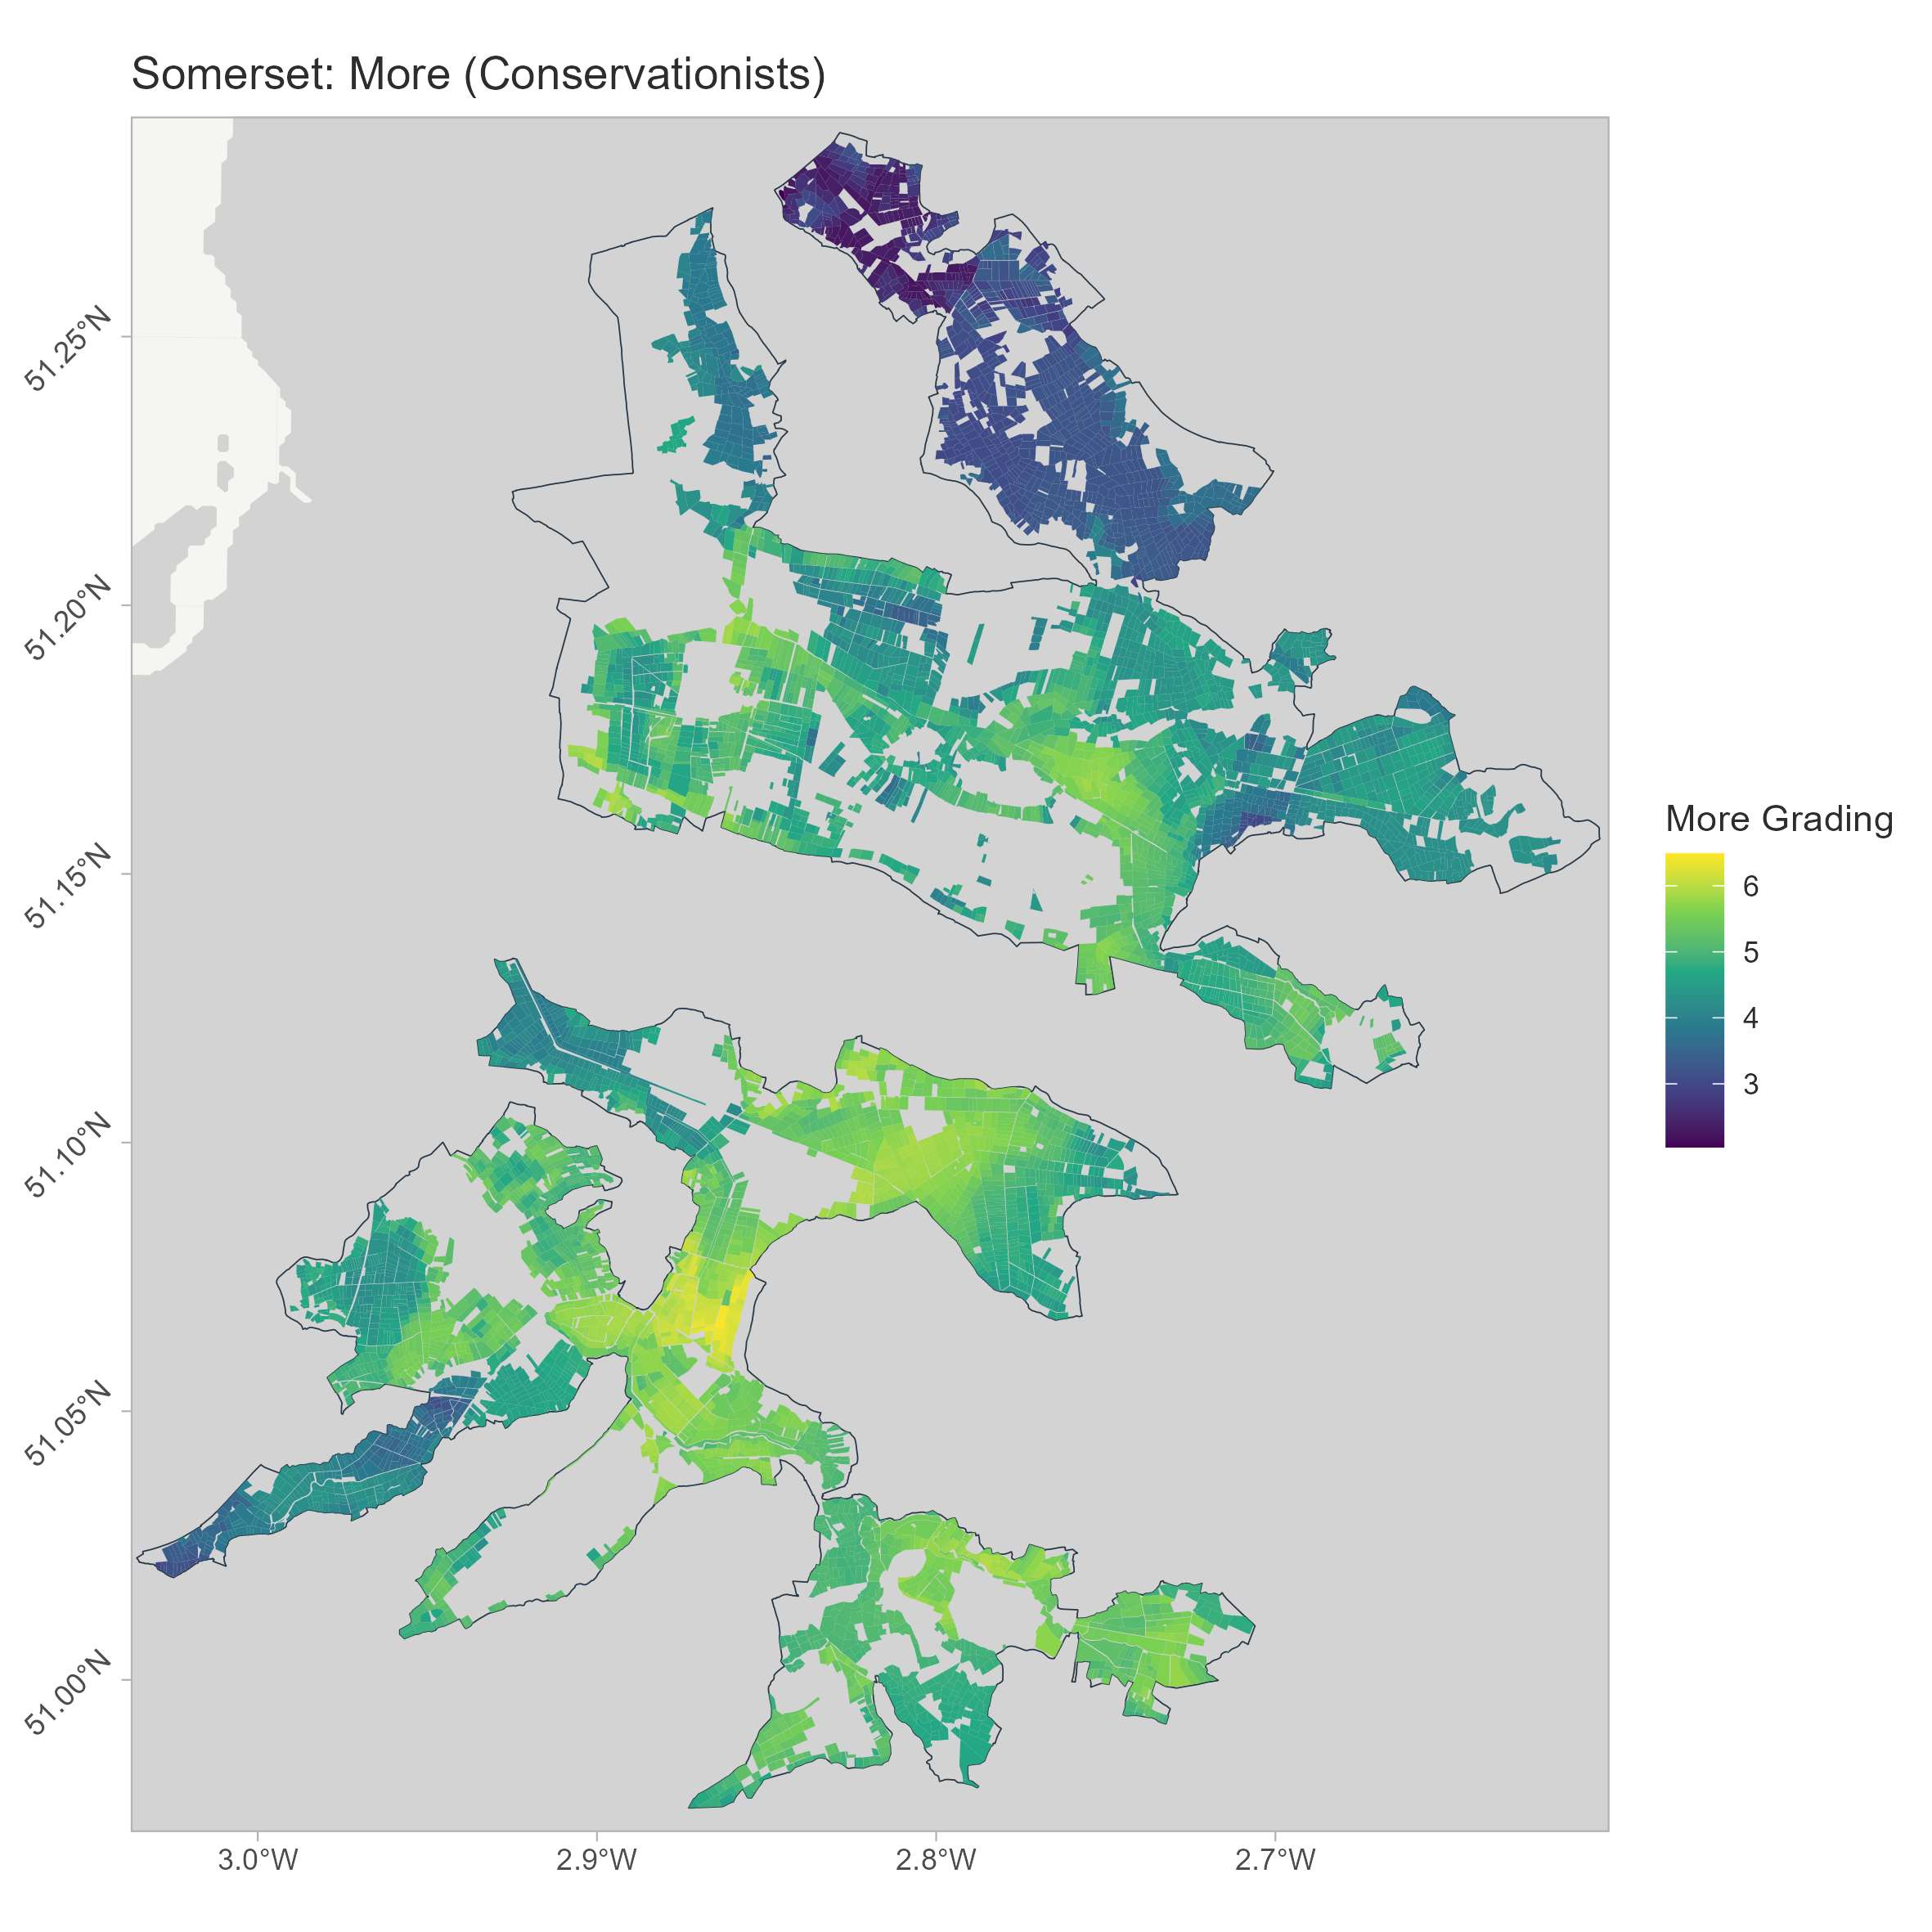
\includegraphics[width=\textwidth,height=9.375in]{Plots/Somerset_G1_More.png}

}

\caption{\label{fig-SomMoreG1}Stakeholder gradings for group 1 in the
Somerset Levels for the more principle of nature restoration}

\end{figure}%

\begin{figure}[H]

\centering{

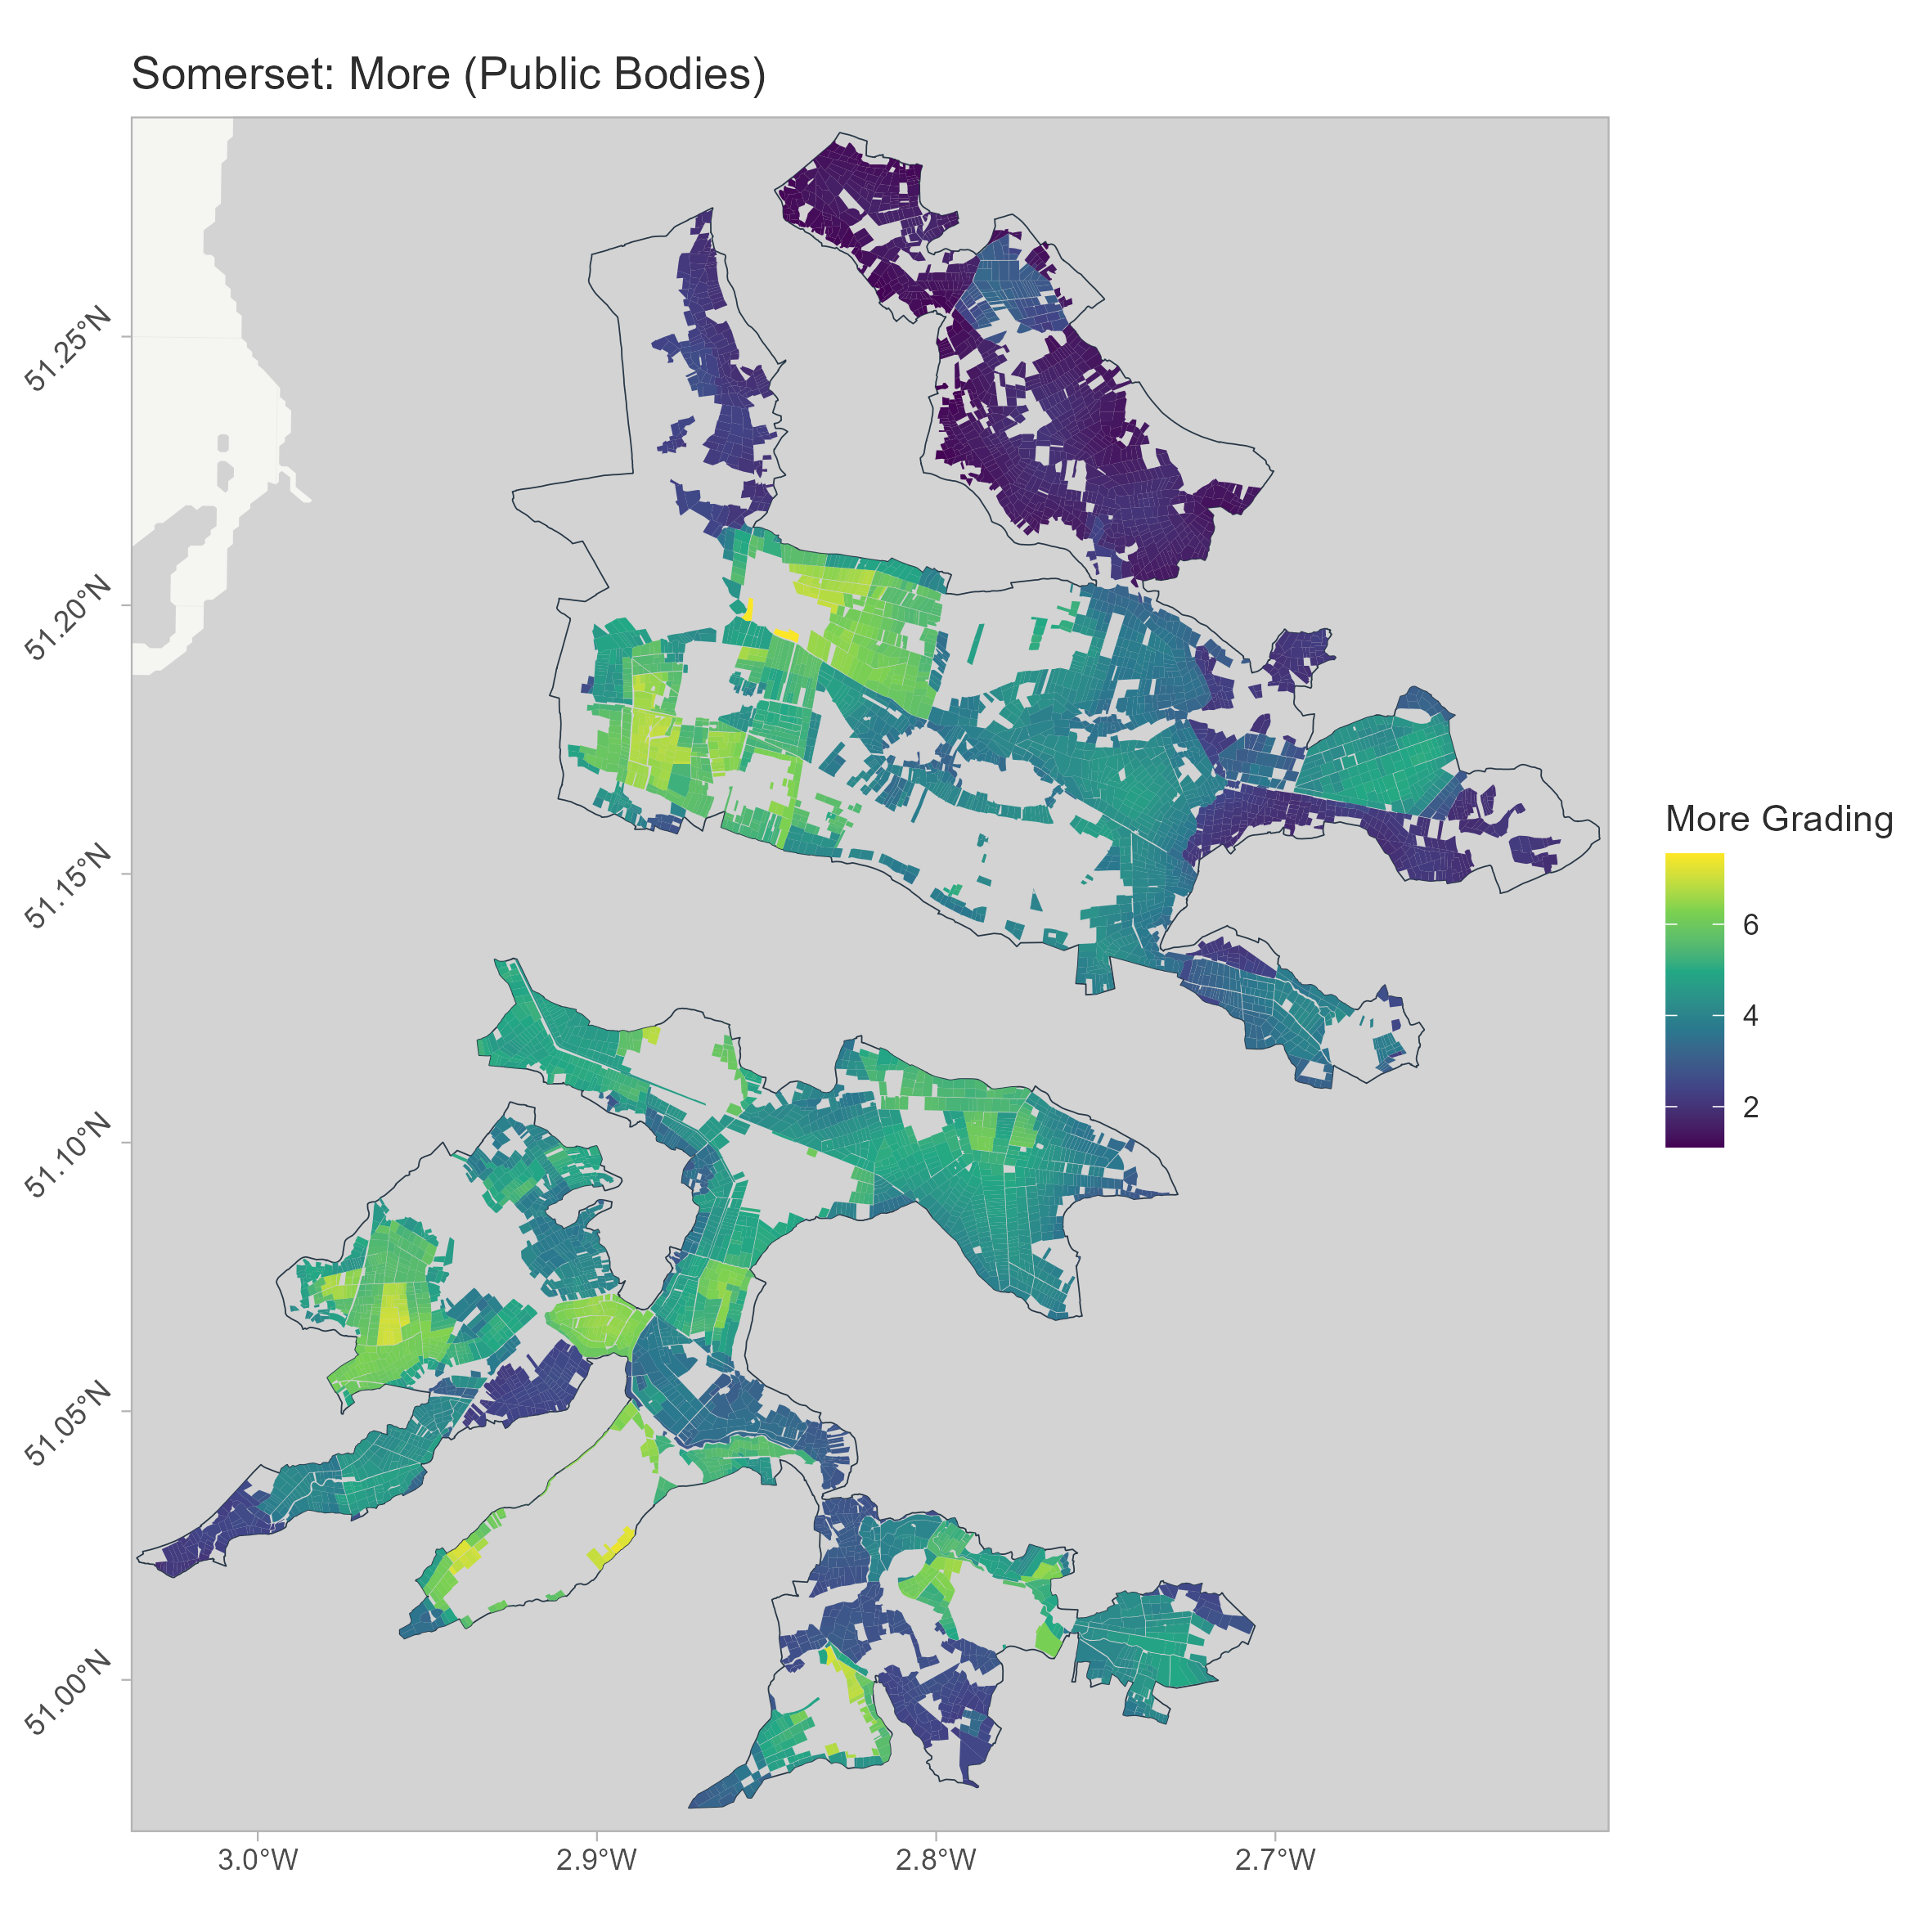
\includegraphics[width=\textwidth,height=9.375in]{Plots/Somerset_G2_More.png}

}

\caption{\label{fig-SomMoreG2}Stakeholder gradings for group 2 in the
Somerset Levels for the more principle of nature restoration}

\end{figure}%

\begin{figure}[H]

\centering{

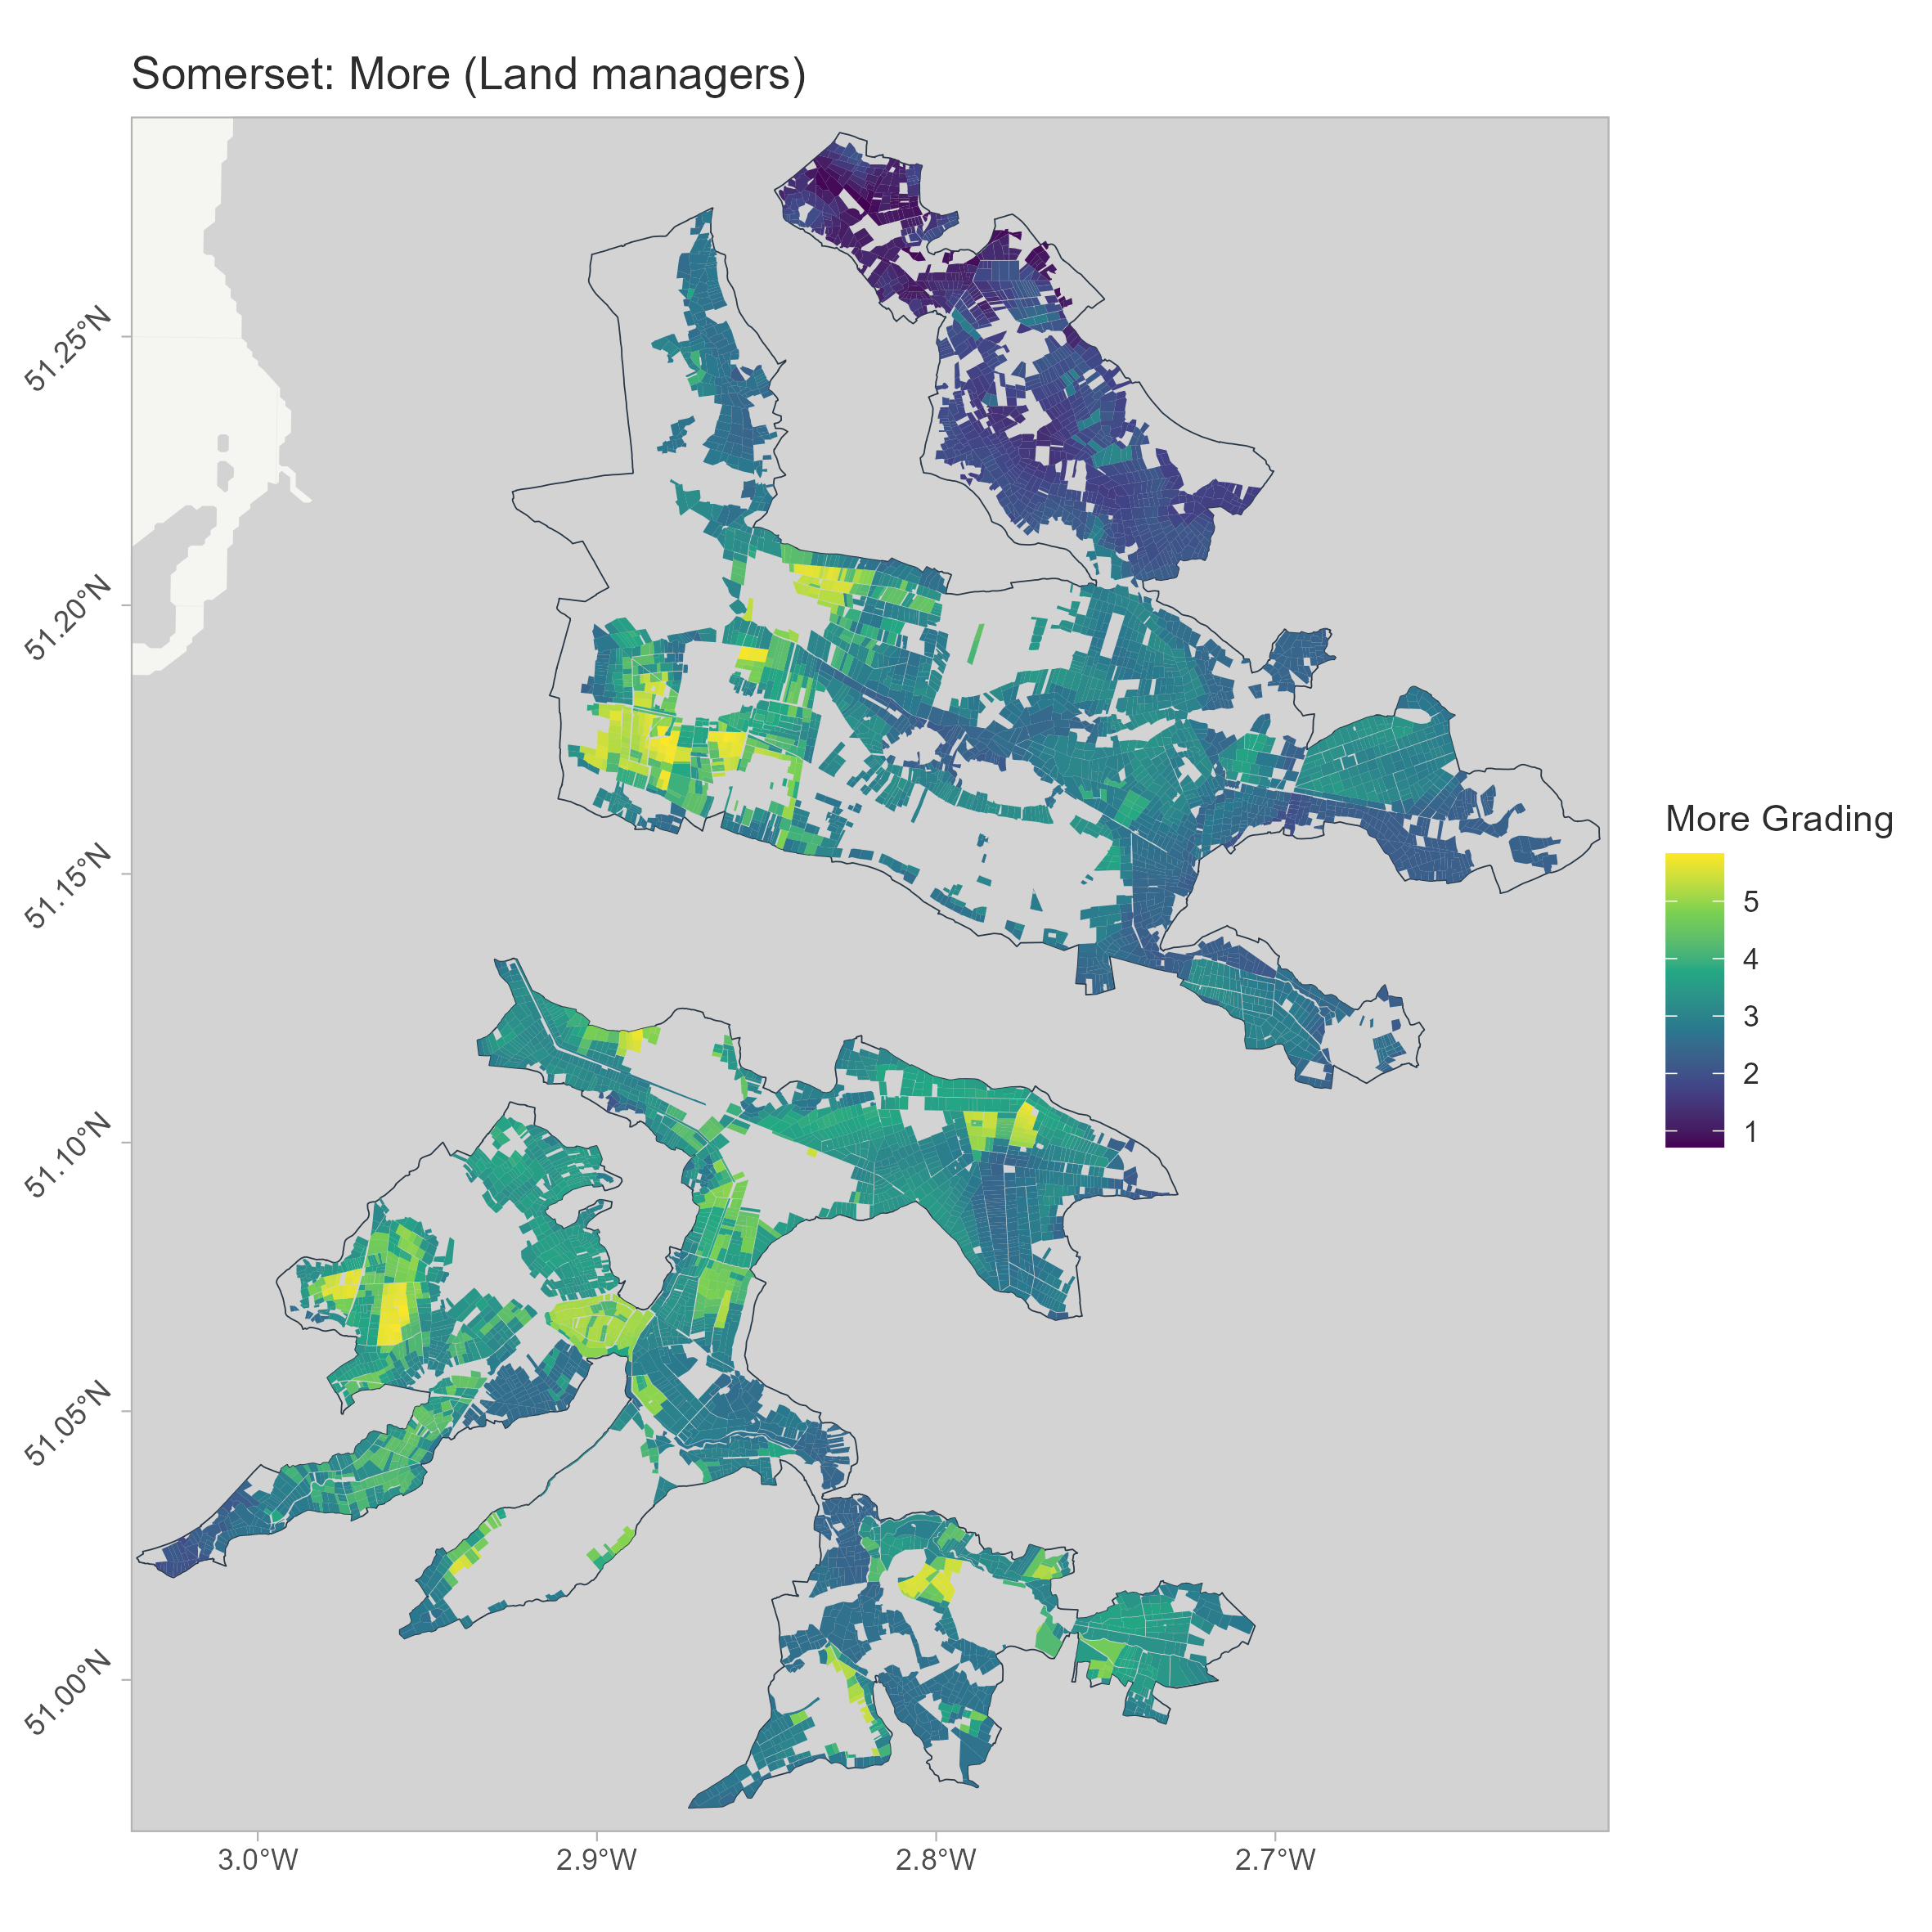
\includegraphics[width=\textwidth,height=9.375in]{Plots/Somerset_G3_More.png}

}

\caption{\label{fig-SomMoreG3}Stakeholder gradings for group 3 in the
Somerset Levels for the more principle of nature restoration}

\end{figure}%

\newpage{}

\paragraph{Somerset Levels: Arable Reversion for
Bigger}\label{somerset-levels-arable-reversion-for-bigger}

The stakeholder preferences for the reversion of arable land to lowland
wet grassland under the bigger principle of nature restoration for group
1 (Figure~\ref{fig-SomArBigG1}), group 2 (Figure~\ref{fig-SomArBigG2})
and group 3 (Figure~\ref{fig-SomArBigG3}).

\begin{figure}[H]

\centering{

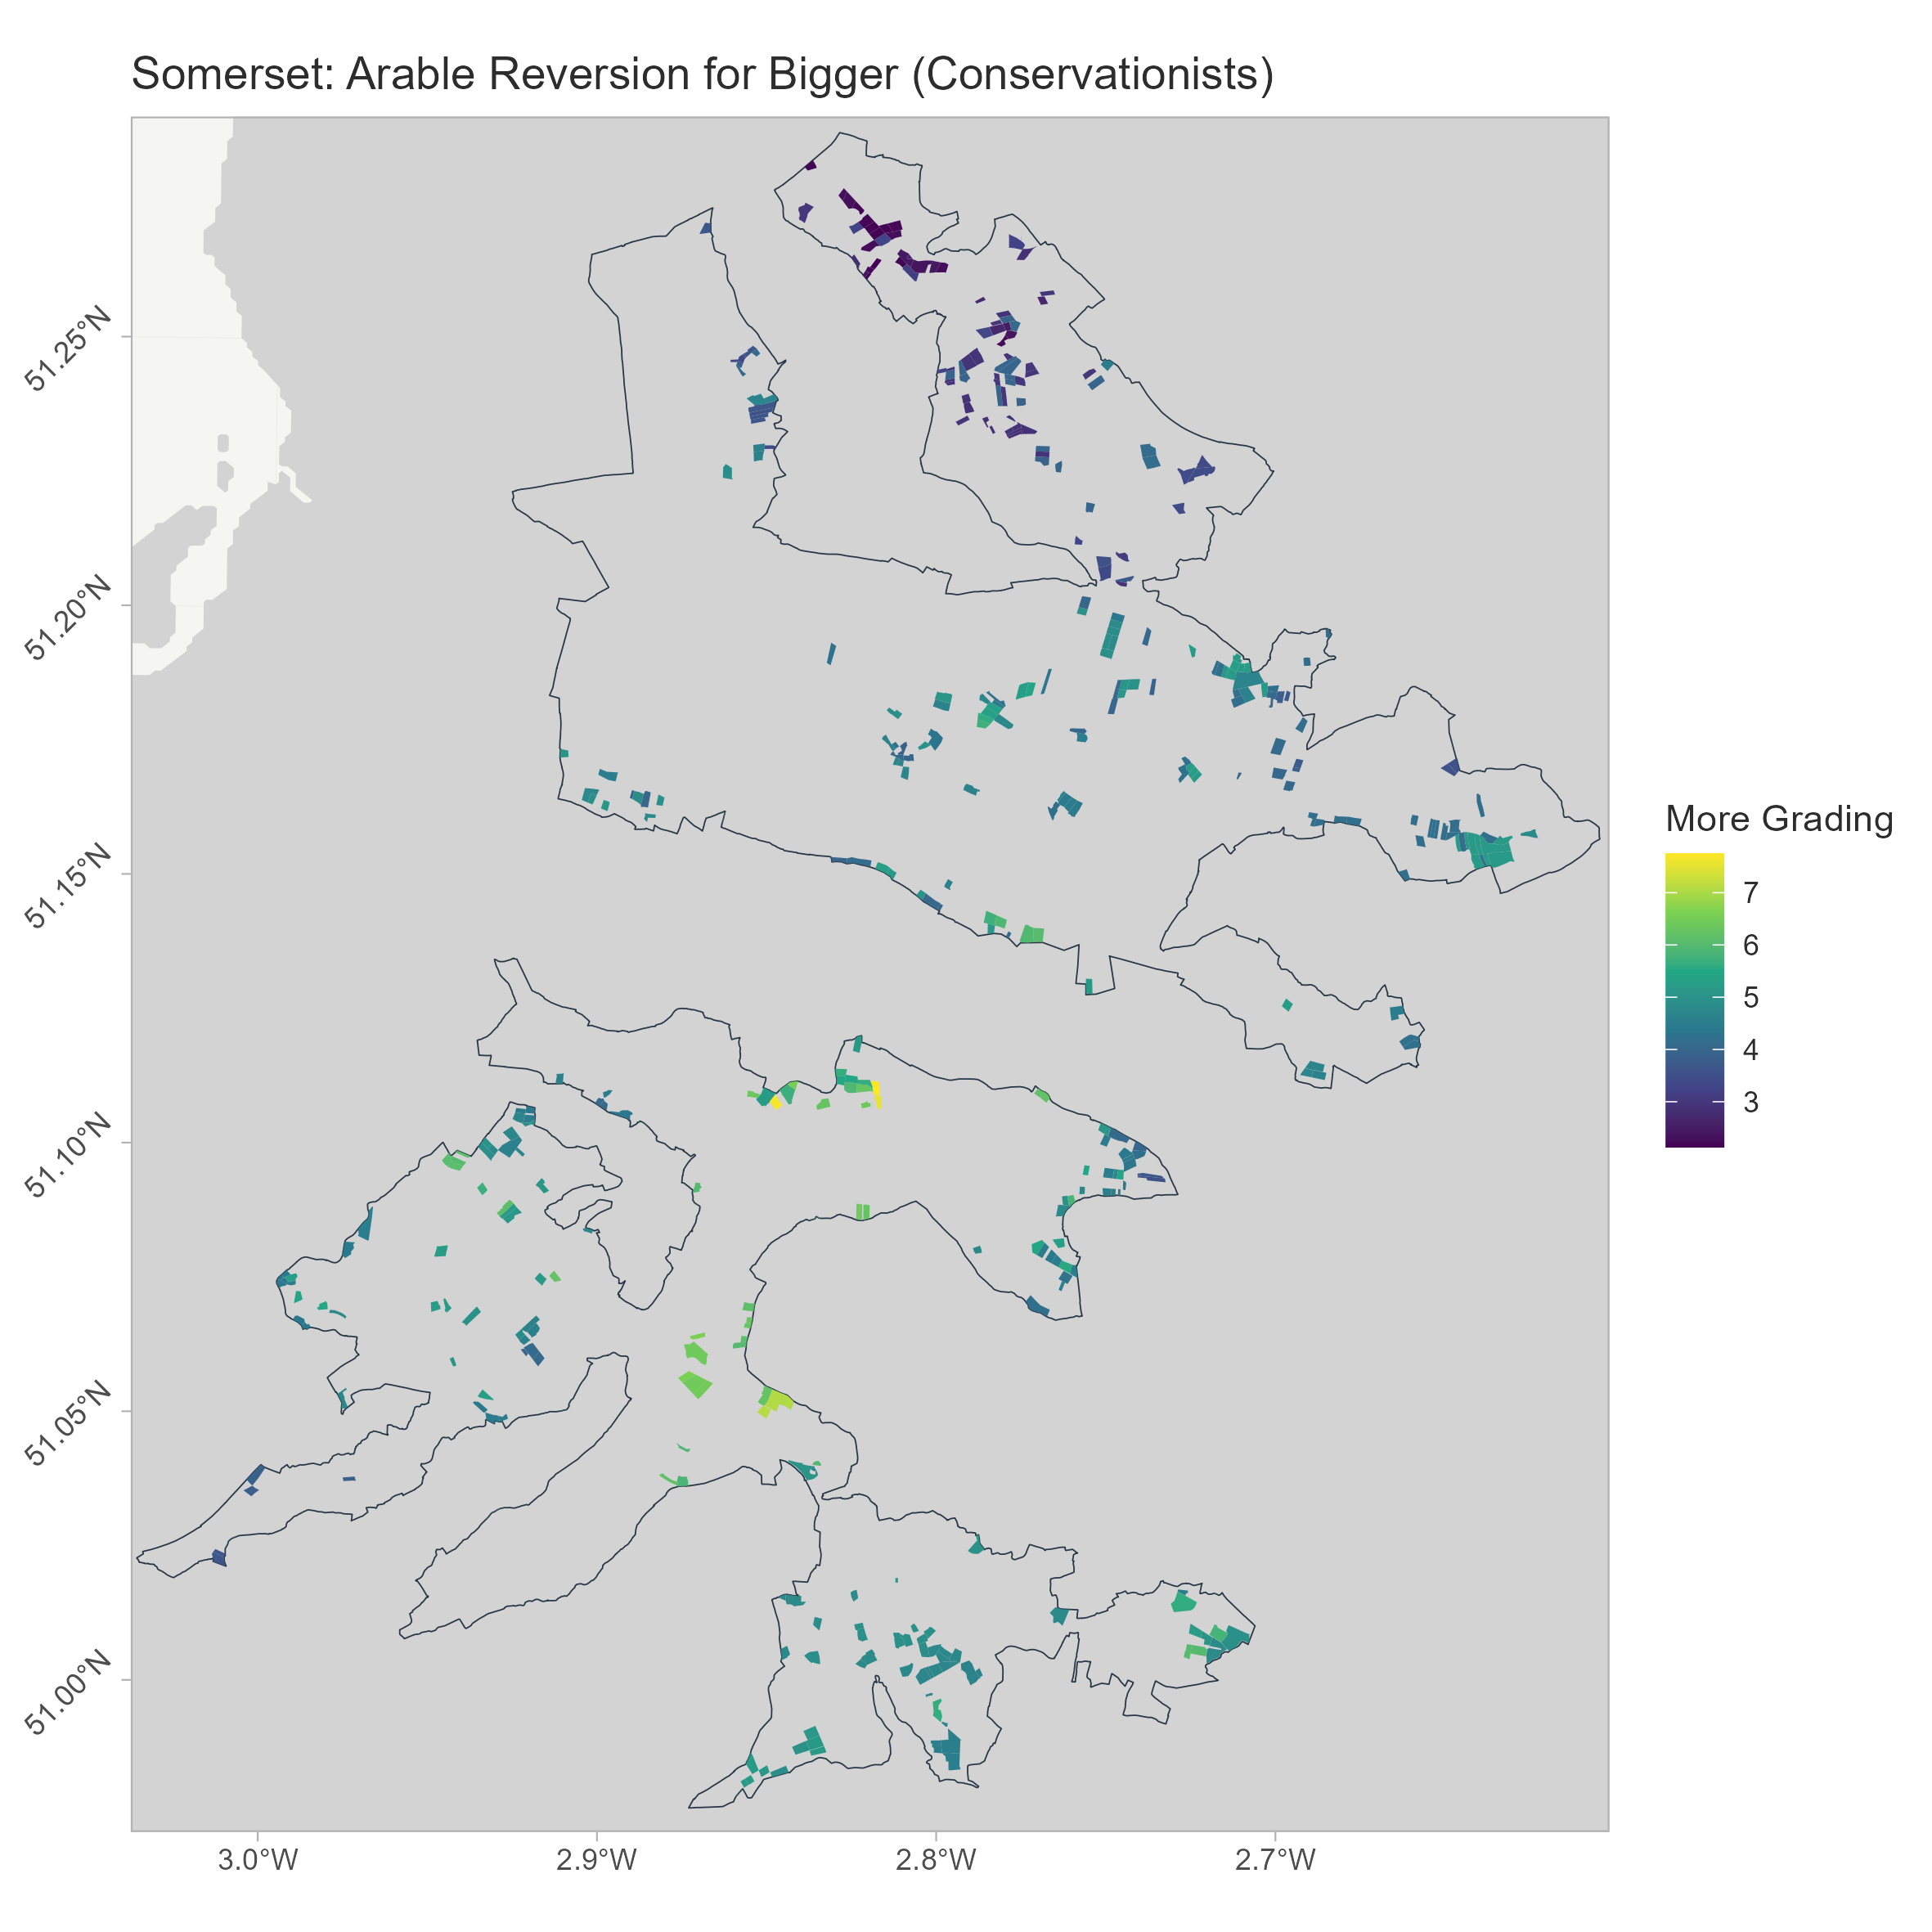
\includegraphics[width=\textwidth,height=9.375in]{Plots/Somerset_G1_ArableBig.png}

}

\caption{\label{fig-SomArBigG1}Stakeholder gradings for group 1 in the
Somerset Levels for the reversion of arable land to lowland wet
grassland under the bigger principle of nature restoration}

\end{figure}%

\begin{figure}[H]

\centering{

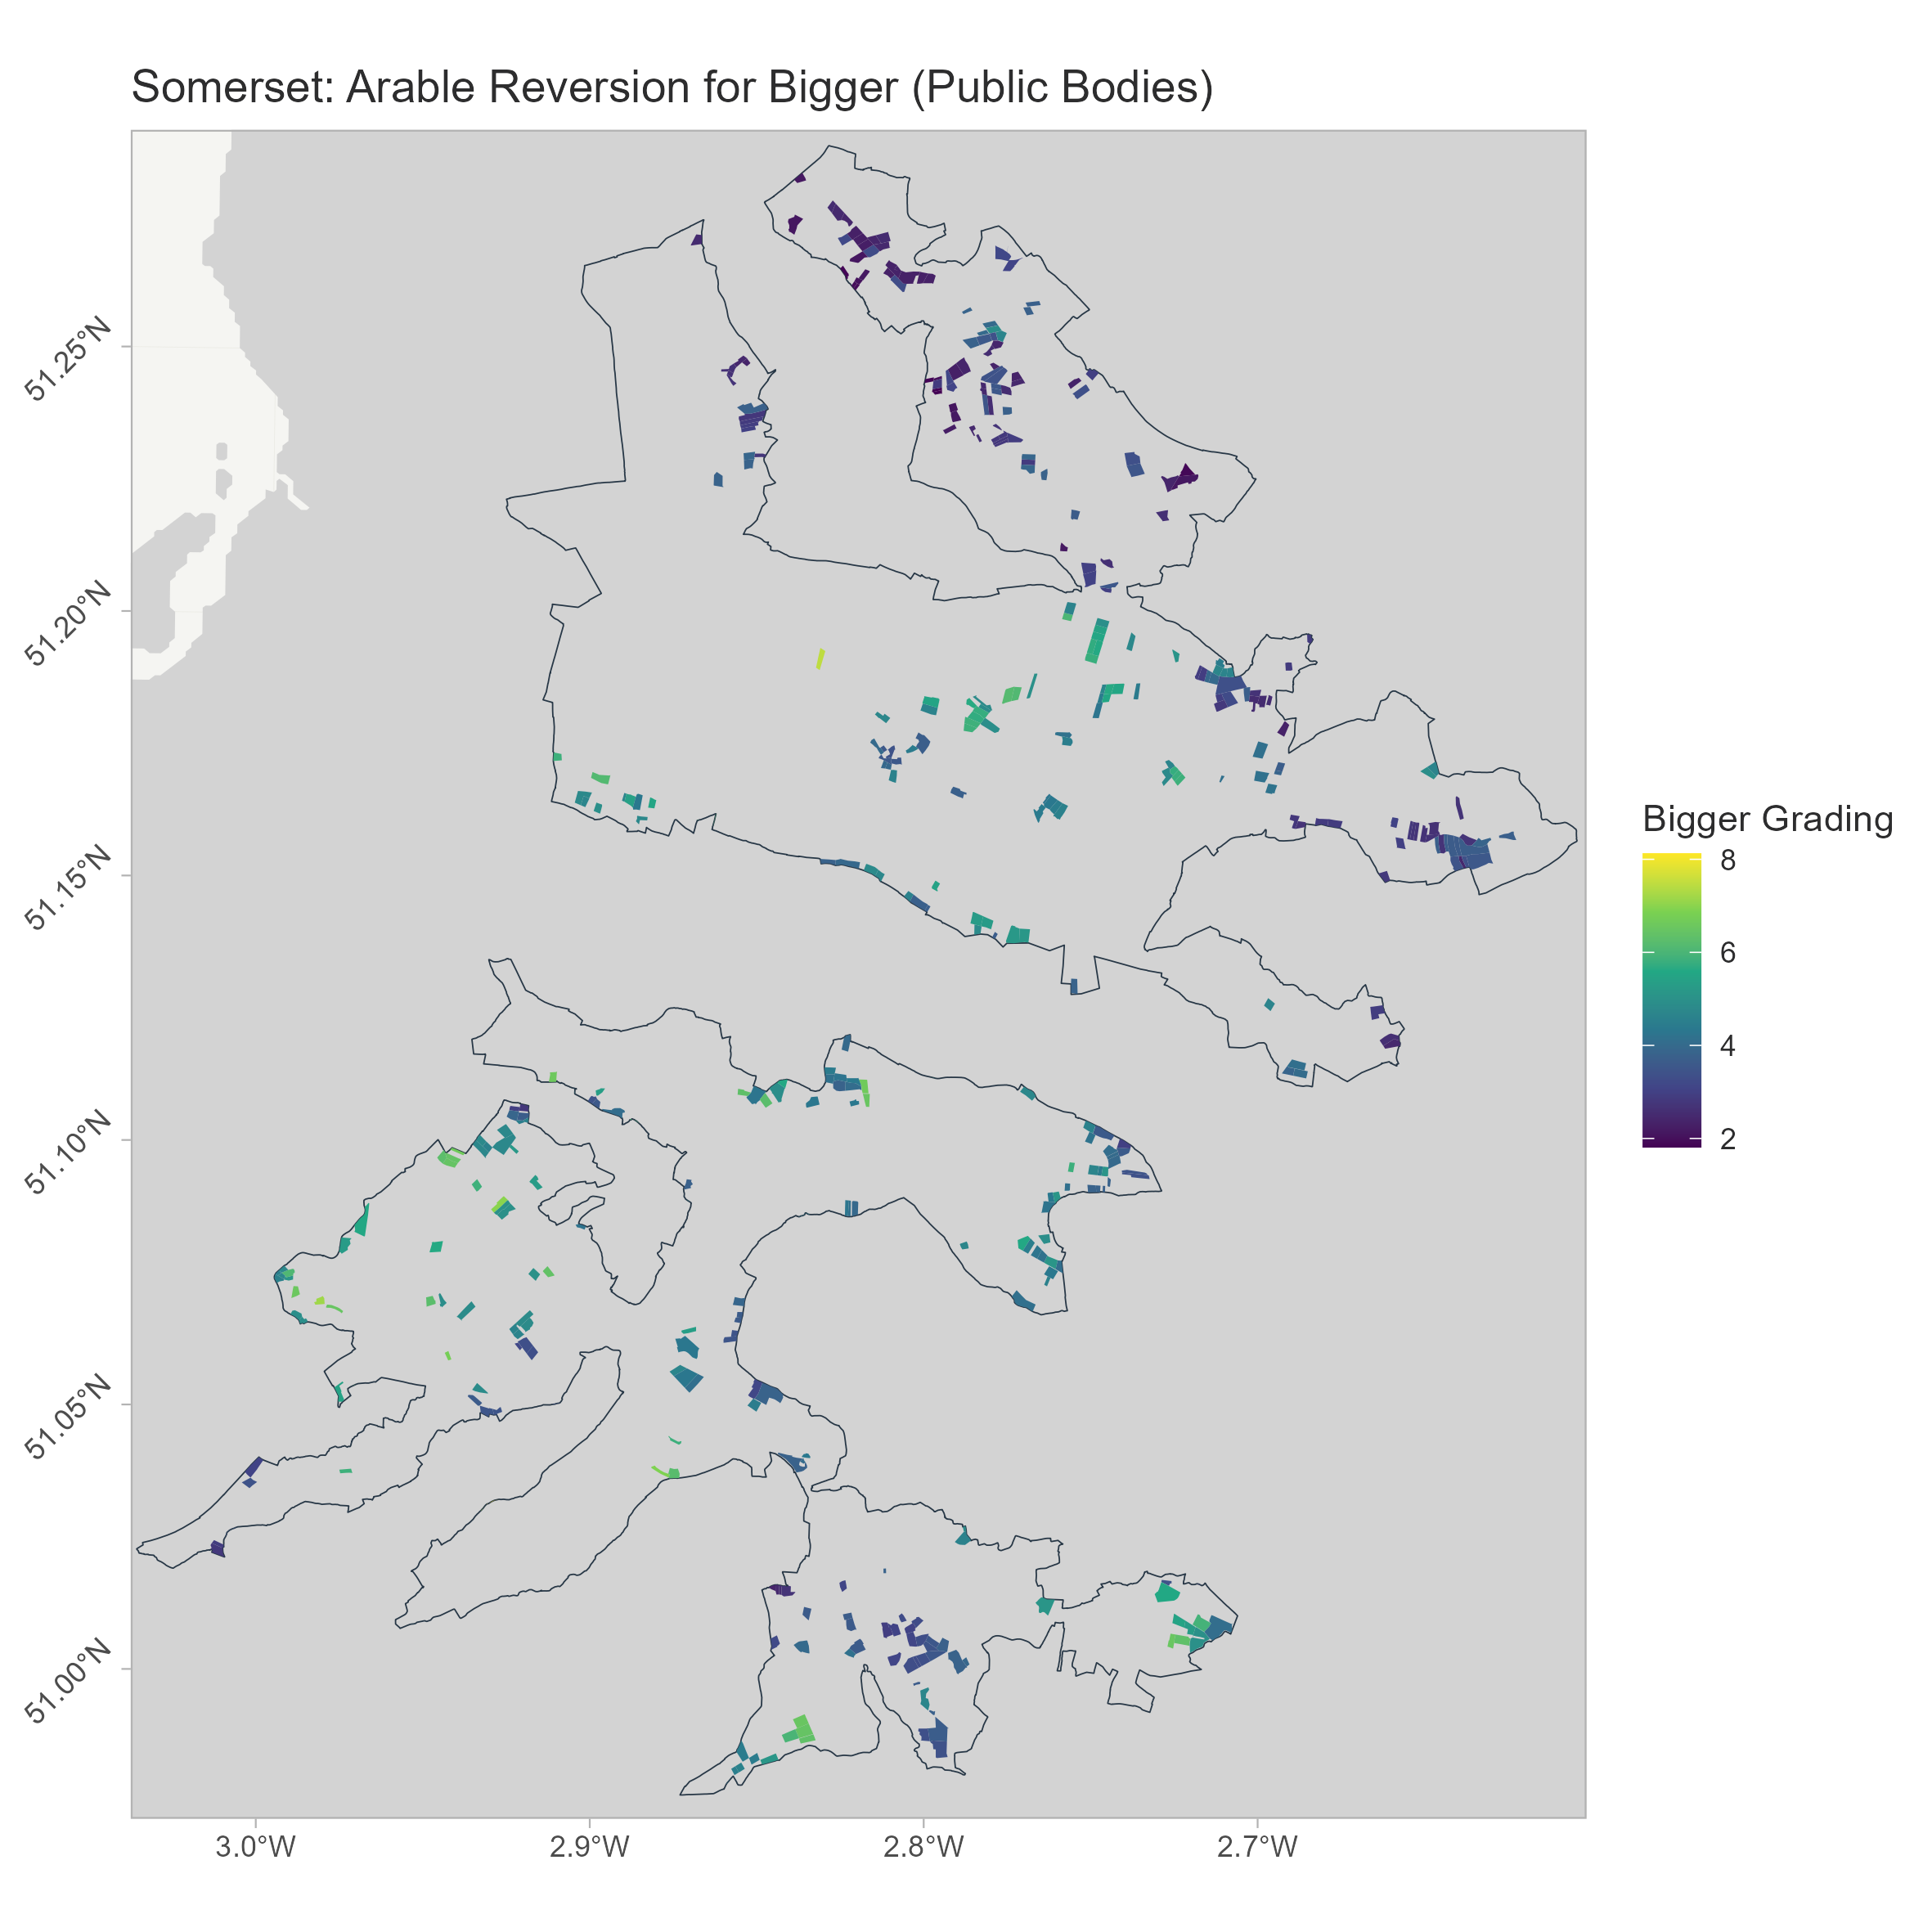
\includegraphics[width=\textwidth,height=9.375in]{Plots/Somerset_G2_ArableBig.png}

}

\caption{\label{fig-SomArBigG2}Stakeholder gradings for group 2 in the
Somerset Levels for the reversion of arable land to lowland wet
grassland under the bigger principle of nature restoration}

\end{figure}%

\begin{figure}[H]

\centering{

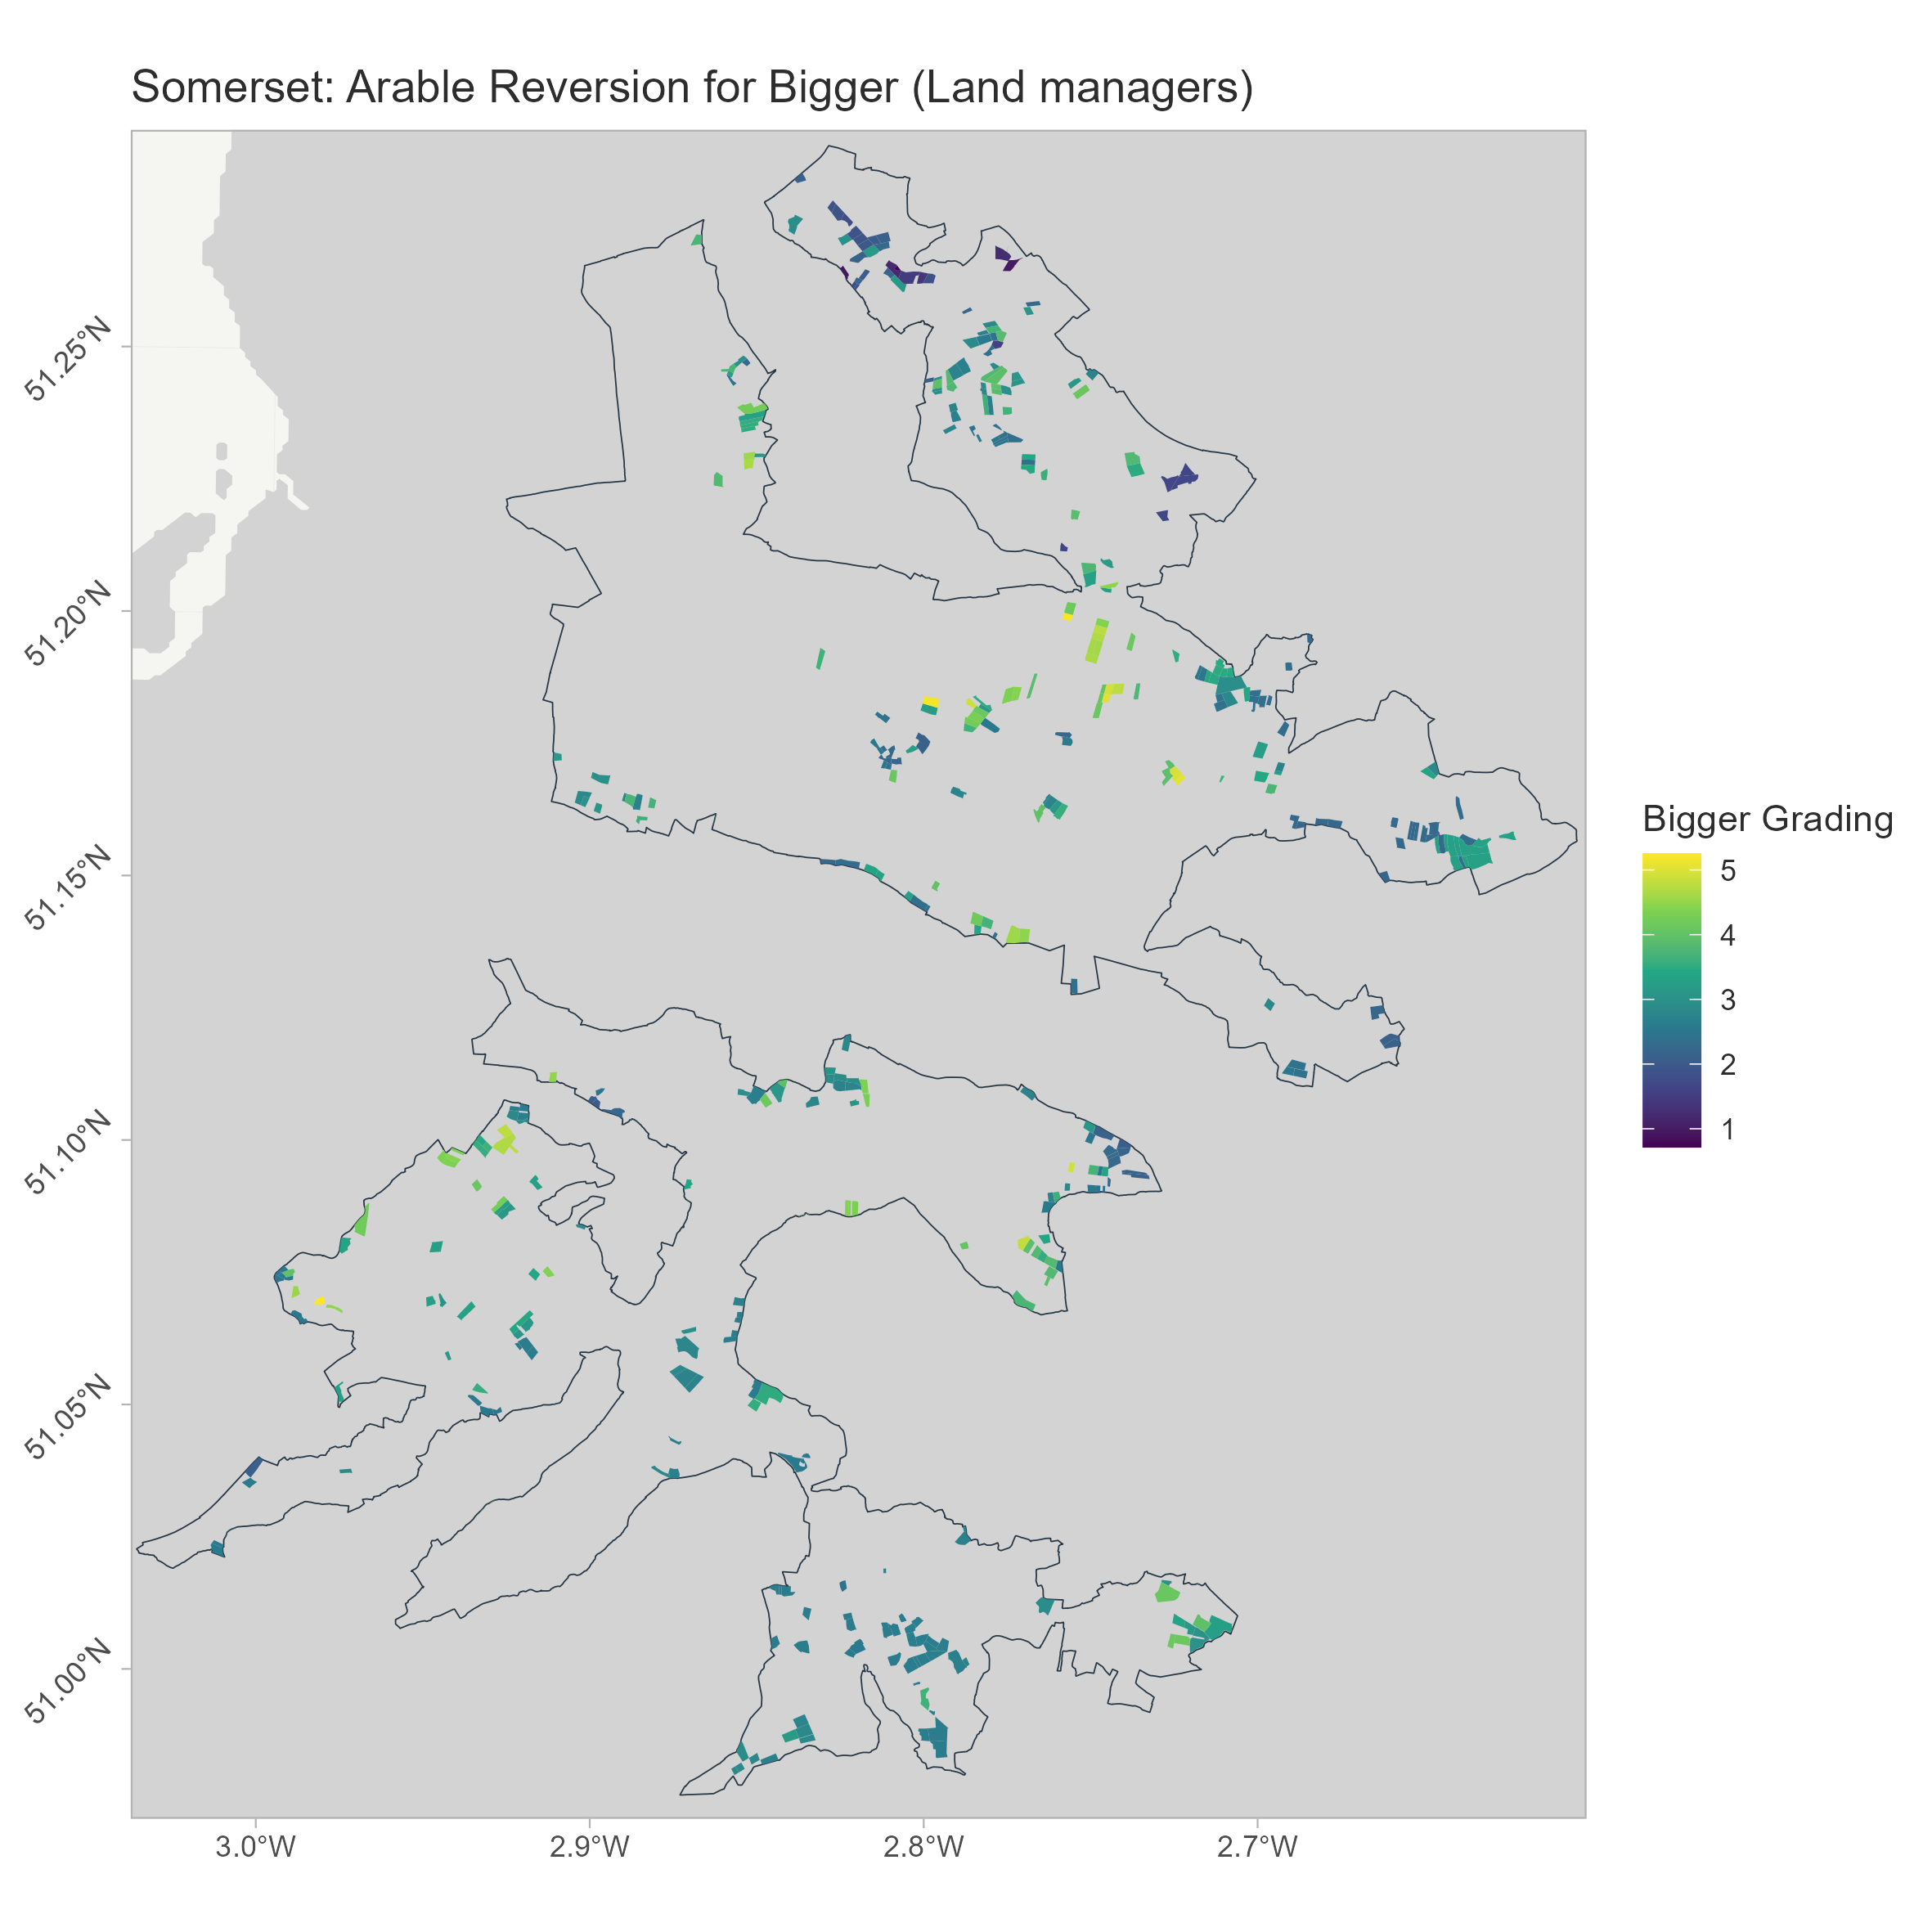
\includegraphics[width=\textwidth,height=9.375in]{Plots/Somerset_G3_ArableBig.png}

}

\caption{\label{fig-SomArBigG3}Stakeholder gradings for group 3 in the
Somerset Levels for the the reversion of arable land to lowland wet
grassland under bigger principle of nature restoration}

\end{figure}%

\newpage{}

\paragraph{Somerset Levels: Arable Reversion for
More}\label{somerset-levels-arable-reversion-for-more}

The stakeholder preferences for the reversion of arable land to lowland
wet grassland under the more principle of nature restoration for group 1
(Figure~\ref{fig-SomArMoreG1}), group 2 (Figure~\ref{fig-SomArMoreG2})
and group 3 (Figure~\ref{fig-SomArMoreG3}).

\begin{figure}[H]

\centering{

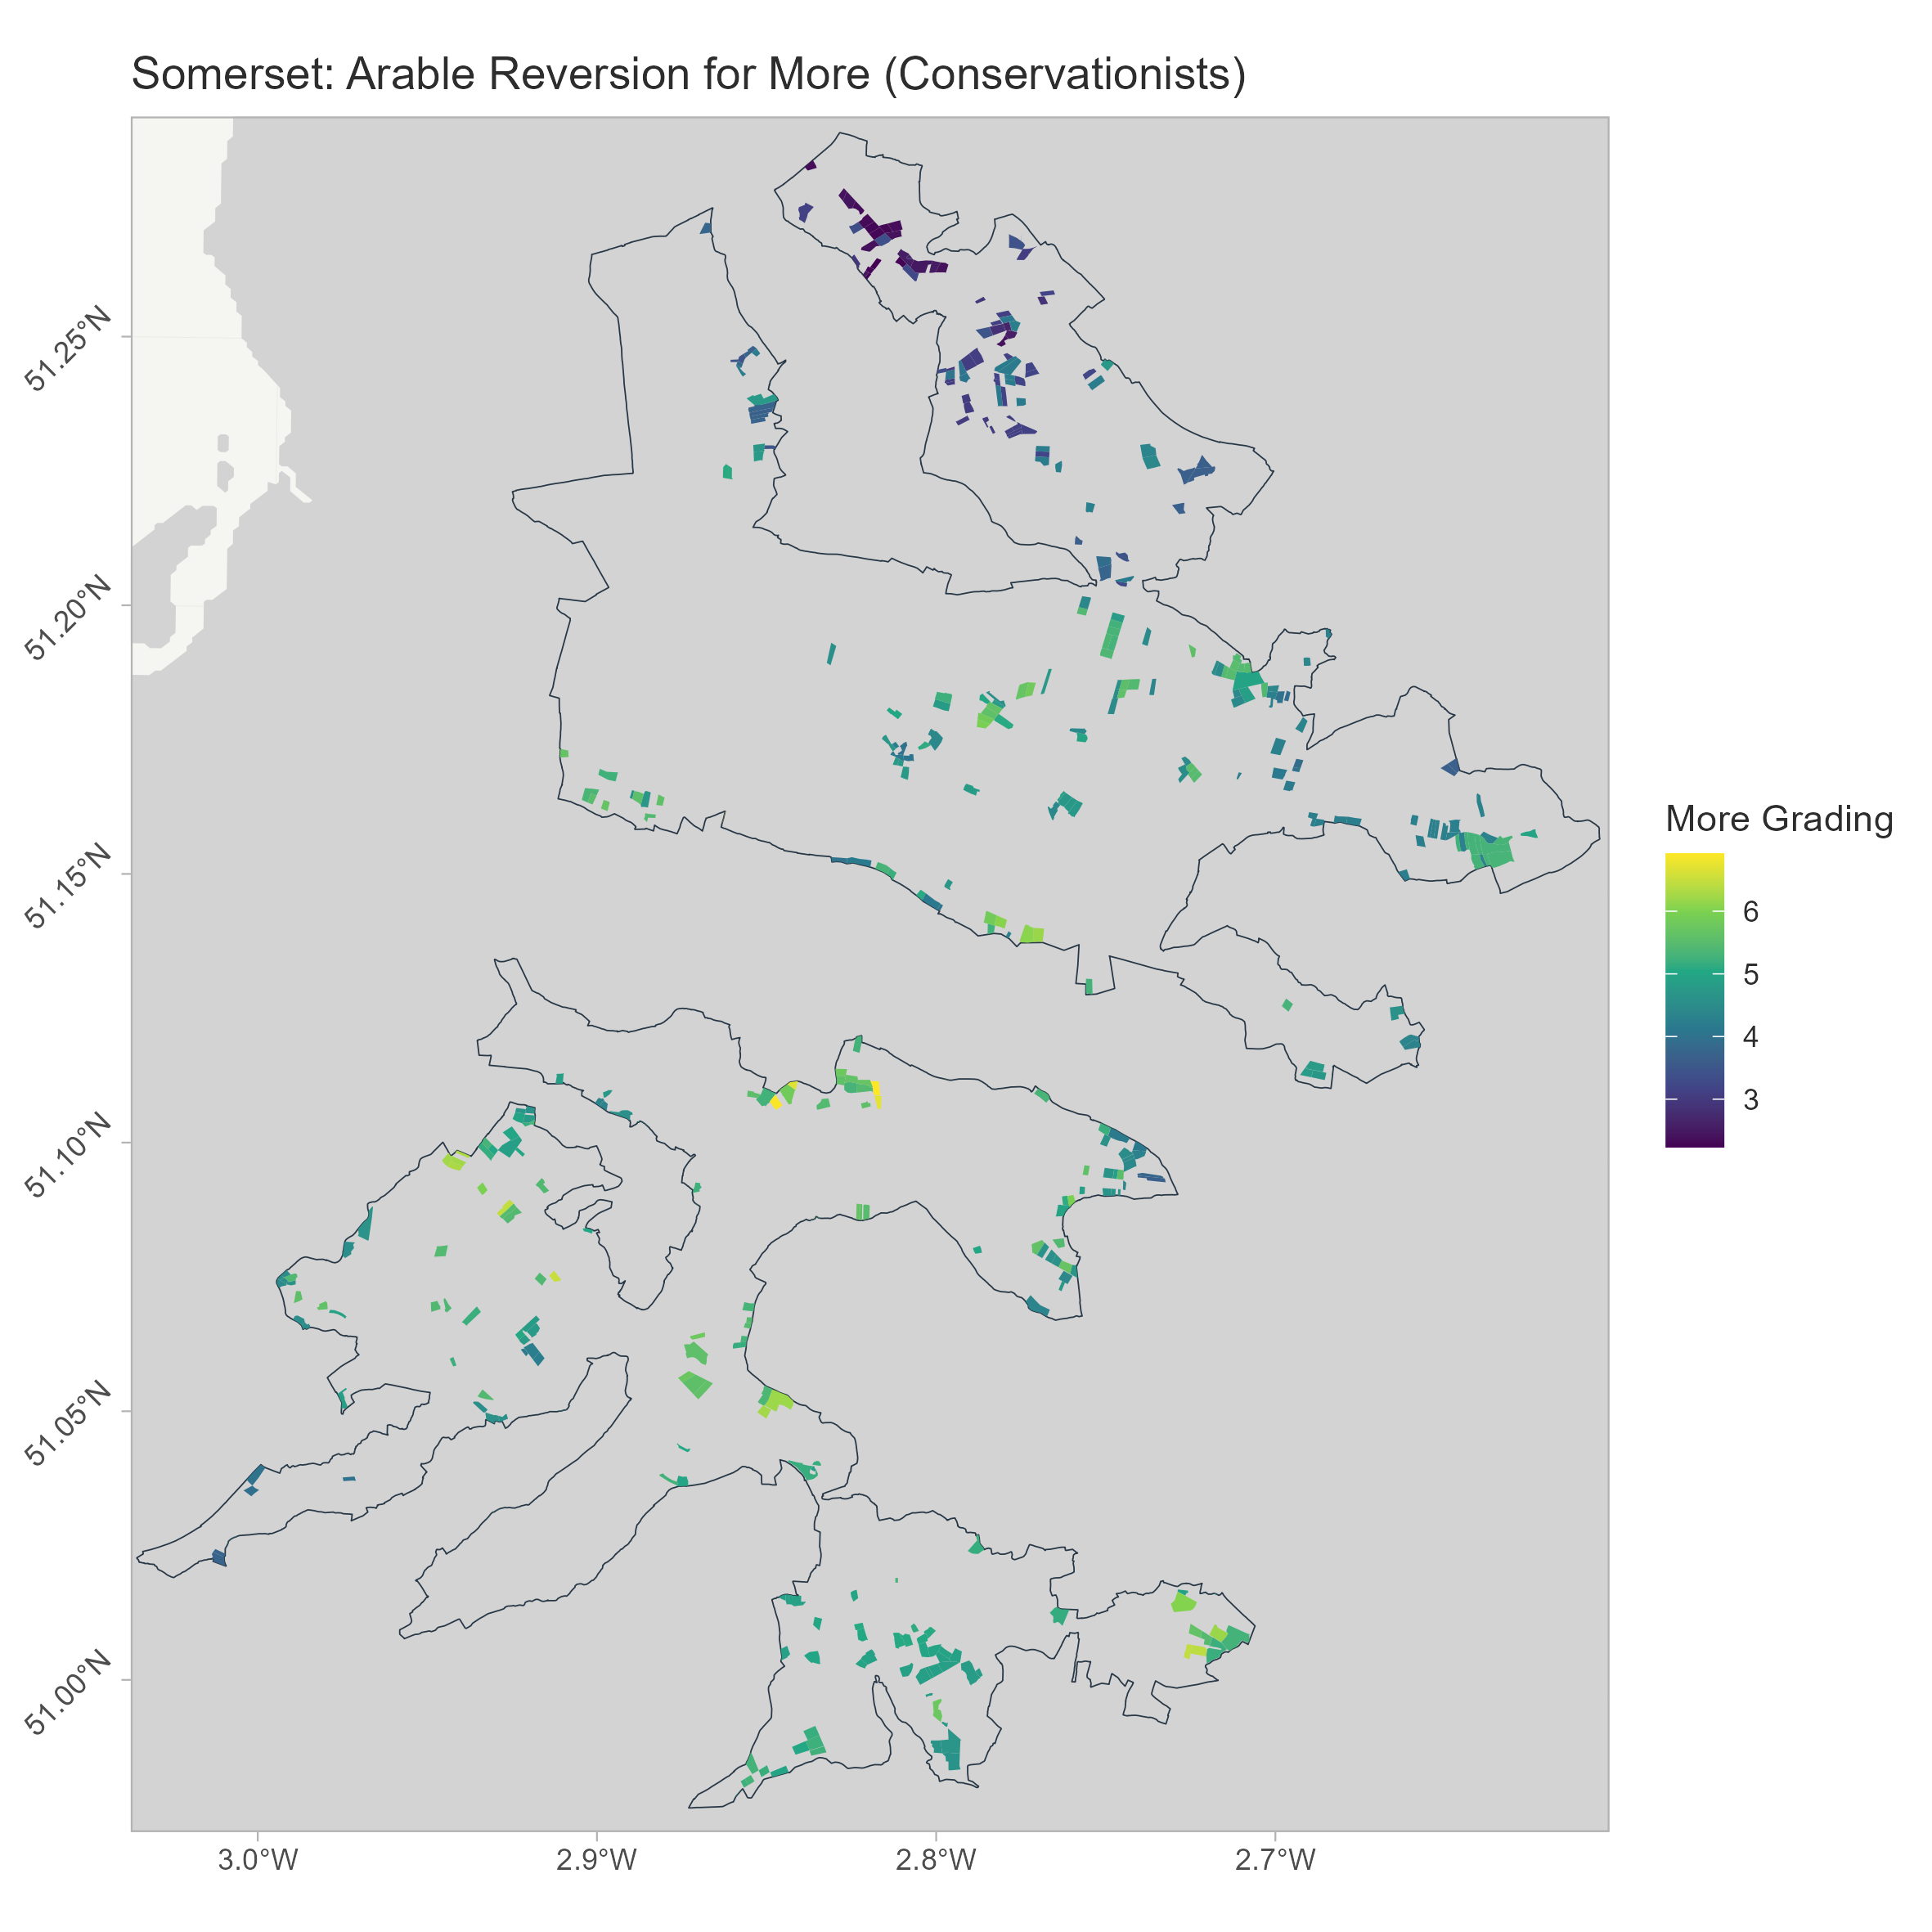
\includegraphics[width=\textwidth,height=9.375in]{Plots/Somerset_G1_ArableMore.png}

}

\caption{\label{fig-SomArMoreG1}Stakeholder gradings for group 1 in the
Somerset Levels for the reversion of arable land to lowland wet
grassland under the bigger principle of nature restoration}

\end{figure}%

\begin{figure}[H]

\centering{

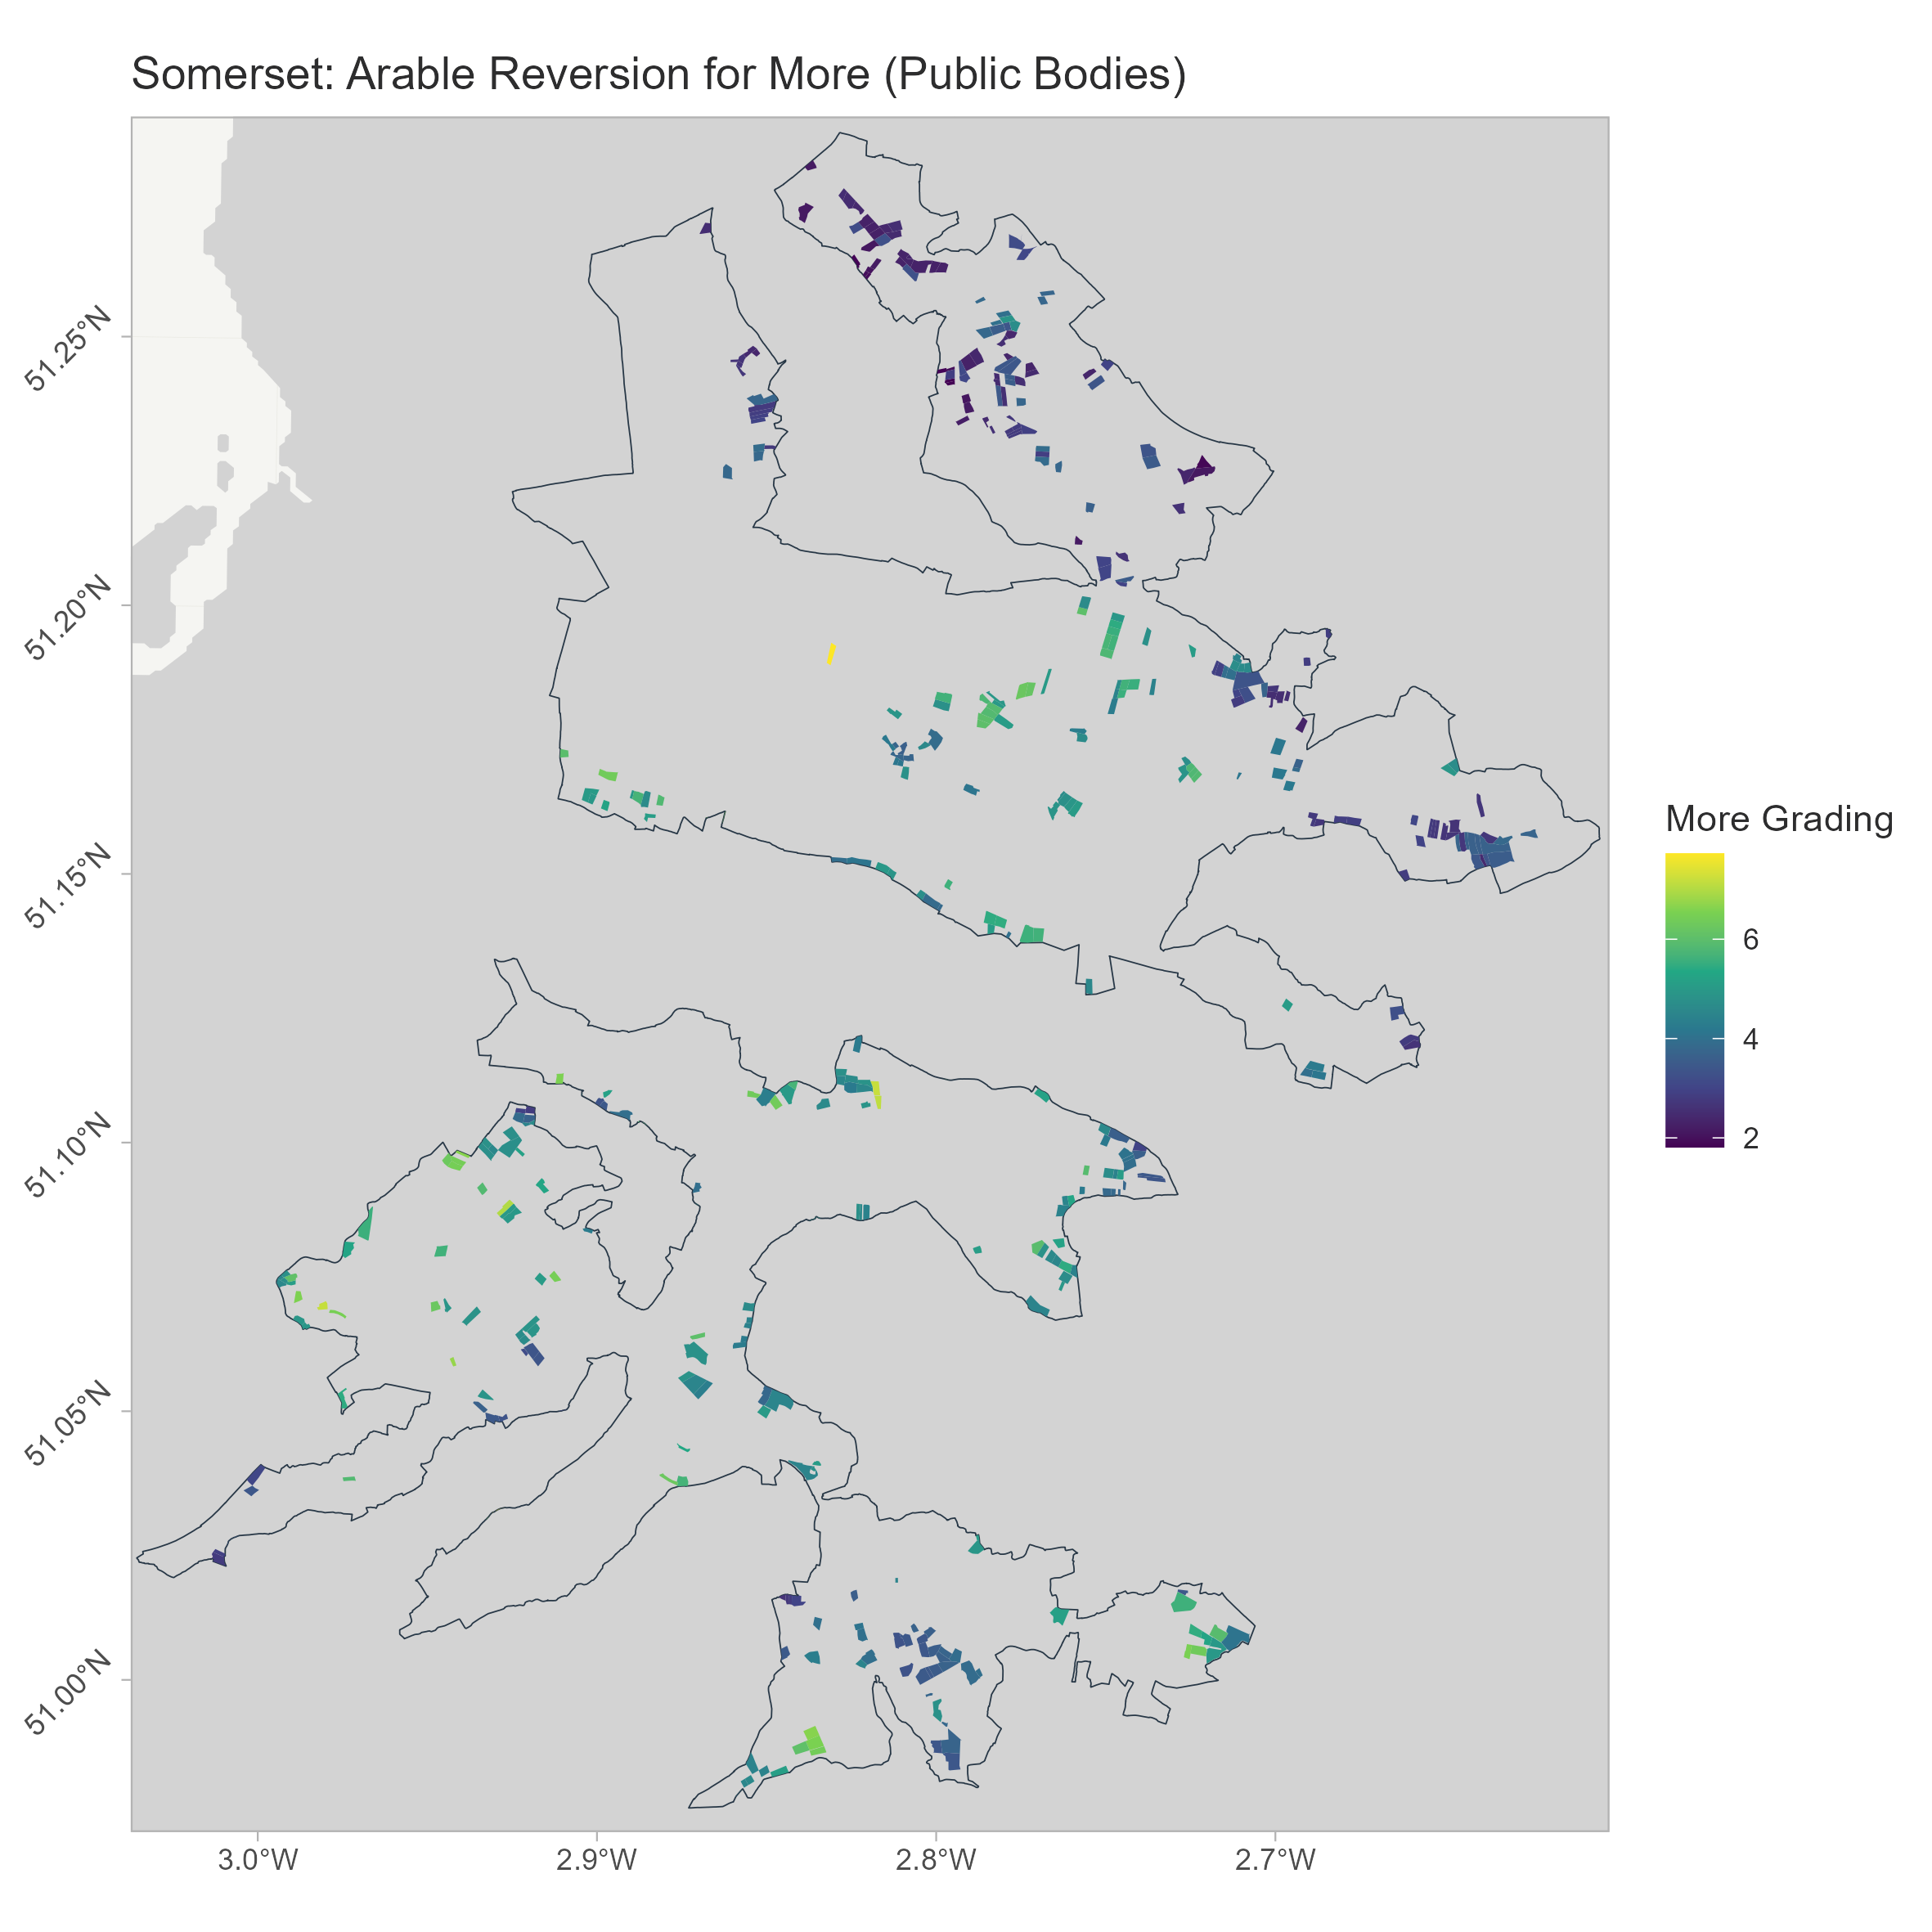
\includegraphics[width=\textwidth,height=9.375in]{Plots/Somerset_G2_ArableMore.png}

}

\caption{\label{fig-SomArMoreG2}Stakeholder gradings for group 2 in the
Somerset Levels for the reversion of arable land to lowland wet
grassland under the bigger principle of nature restoration}

\end{figure}%

\begin{figure}[H]

\centering{

\includegraphics[width=\textwidth,height=9.375in]{Plots/Somerset_G3_ArableMore.png}

}

\caption{\label{fig-SomArMoreG3}Stakeholder gradings for group 3 in the
Somerset Levels for the the reversion of arable land to lowland wet
grassland under bigger principle of nature restoration}

\end{figure}%

\newpage{}

\subsection{Acknowledgements}\label{acknowledgements}

We thank thank all the workshop attendees, and a specific thanks to
Damon Bridge, Kieran Alexander, Will Tofts, Ian Robinson, Alan Johnson
and Mark Smart for helping to organise these workshops. We also thank
Malcolm Ausden and the wider lowland wader scenario steering group team
for input into the project. We also need to thank NE for funding.

\newpage{}

\subsection*{Bibliography}\label{bibliography}
\addcontentsline{toc}{subsection}{Bibliography}

\phantomsection\label{refs}
\begin{CSLReferences}{1}{0}
\bibitem[\citeproctext]{ref-chazdon2016}
Chazdon, Robin L., Pedro H. S. Brancalion, David Lamb, Lars Laestadius,
Miguel Calmon, and Chetan Kumar. 2016. {``A Policy{-}Driven Knowledge
Agenda for Global Forest and Landscape Restoration.''}
\emph{Conservation Letters} 10 (1): 125--32.
\url{https://doi.org/10.1111/conl.12220}.

\bibitem[\citeproctext]{ref-donald2001}
Donald, P. F., R. E. Green, and M. F. Heath. 2001. {``Agricultural
Intensification and the Collapse of Europe's Farmland Bird
Populations.''} \emph{Proceedings of the Royal Society of London. Series
B: Biological Sciences} 268 (1462): 25--29.
\url{https://doi.org/10.1098/rspb.2000.1325}.

\bibitem[\citeproctext]{ref-eglington2010}
Eglington, Sarah M., Mark Bolton, Mark A. Smart, William J. Sutherland,
Andrew R. Watkinson, and Jennifer A. Gill. 2010. {``Managing Water
Levels on Wet Grasslands to Improve Foraging Conditions for Breeding
Northern Lapwing{\emph{Vanellus Vanellus}}.''} \emph{Journal of Applied
Ecology} 47 (2): 451--58.
\url{https://doi.org/10.1111/j.1365-2664.2010.01783.x}.

\bibitem[\citeproctext]{ref-envagency2023a}
Environment Agency. 2023a. \emph{LIDAR Composite Digital Terrain Model
(DTM) - 1m}.
\url{https://environment.data.gov.uk/dataset/13787b9a-26a4-4775-8523-806d13af58fc}.

\bibitem[\citeproctext]{ref-envagency2023b}
---------. 2023b. \emph{LIDAR Composite First Return Digital Surface
Model (FZ\_DSM) - 1m}.
\url{https://environment.data.gov.uk/dataset/df4e3ec3-315e-48aa-aaaf-b5ae74d7b2bb}.

\bibitem[\citeproctext]{ref-franks2018}
Franks, Samantha E., Maja Roodbergen, Wolf Teunissen, Anne Carrington
Cotton, and James W. Pearce-Higgins. 2018. {``Evaluating the
Effectiveness of Conservation Measures for European Grassland{-}Breeding
Waders.''} \emph{Ecology and Evolution} 8 (21): 10555--68.
\url{https://doi.org/10.1002/ece3.4532}.

\bibitem[\citeproctext]{ref-gamborg2019}
Gamborg, Christian, Jonas Morsing, and Karsten Raulund-Rasmussen. 2019.
{``Adjustive Ecological Restoration Through Stakeholder Involvement: A
Case of Riparian Landscape Restoration on Privately Owned Land with
Public Access.''} \emph{Restoration Ecology} 27 (5): 1073--83.
\url{https://doi.org/10.1111/rec.12955}.

\bibitem[\citeproctext]{ref-hijmans2024}
Hijmans, R. J. 2024. \emph{Terra: Spatial Data Analysis}.
\url{https://CRAN.R-project.org/package=terra}.

\bibitem[\citeproctext]{ref-lawton2010}
Lawton, J. H., P. N. M. Brotherton, V. K. Brown, C. Elphick, A. H.
Fitter, J. Forshaw, R. W. Haddow, et al. 2010. {``Making Space for
Nature: A Review of England's Wildlife Sites and Ecological Network.
Report to Defra.''}

\bibitem[\citeproctext]{ref-malpas2013}
Malpas, Lucy R., Rosalind J. Kennerley, Graham J. M. Hirons, Rob D.
Sheldon, Malcolm Ausden, Joanne C. Gilbert, and Jennifer Smart. 2013.
{``The Use of Predator-Exclusion Fencing as a Management Tool Improves
the Breeding Success of Waders on Lowland Wet Grassland.''}
\emph{Journal for Nature Conservation} 21 (1): 37--47.
\url{https://doi.org/10.1016/j.jnc.2012.09.002}.

\bibitem[\citeproctext]{ref-marston2024}
Marston, C. G., R. D. Morton, A. W. O'Neil, and C. S. Rowland. 2024.
{``Land Cover Map 2022 (25m Rasterised Land Parcels, GB).''} NERC EDS
Environmental Information Data Centre.
\url{https://doi.org/10.5285/C9449BF5-B8F6-4A1C-B3EB-0D70575CBA39}.

\bibitem[\citeproctext]{ref-marston2022}
Marston, C. G., C. S. Rowland, A. W. O'Neil, and R. D. Morton. 2022.
{``Land Cover Map 2021 (25m Rasterised Land Parcels, GB).''} NERC EDS
Environmental Information Data Centre.
\url{https://doi.org/10.5285/A1F85307-CAD7-4E32-A445-84410EFDFA70}.

\bibitem[\citeproctext]{ref-morton2024}
Morton, R. D., C. G. Marston, A. W. O'Neil, and C. S. Rowland. 2024.
{``Land Cover Map 2023 (25m Rasterised Land Parcels, GB).''} NERC EDS
Environmental Information Data Centre.
\url{https://doi.org/10.5285/AB10EA4A-1788-4D25-A6DF-F1AFF829DFFF}.

\bibitem[\citeproctext]{ref-natengland2022}
Natural England. 2022. \emph{Priority Habitats Inventory (England)}.
\url{https://www.data.gov.uk/dataset/4b6ddab7-6c0f-4407-946e-d6499f19fcde/priority-habitats-inventory-england}.

\bibitem[\citeproctext]{ref-nateng2024}
---------. 2024. \emph{Environmentally Sensitive Areas (England)}.
\href{https://www.data.gov.uk/dataset/a5b0ccc4-a144-4027-91fa-49084ff07da2/environmentally-sensitive-areas-england\%20}{https://www.data.gov.uk/dataset/a5b0ccc4-a144-4027-91fa-49084ff07da2/environmentally-sensitive-areas-england
}.

\bibitem[\citeproctext]{ref-nsri2022}
NSRI. 2022. \emph{National Soil Map of England and Wales - NATMAP
Vector, 1:250000 Soil Association Map}.
\href{https://www.landis.org.uk/data/natmap.cfm\%20}{https://www.landis.org.uk/data/natmap.cfm
}.

\bibitem[\citeproctext]{ref-pebesma2018}
Pebesma, E. 2018. {``{Simple Features for R: Standardized Support for
Spatial Vector Data}.''} \emph{{The R Journal}} 10 (1): 439--46.
\url{https://doi.org/10.32614/RJ-2018-009}.

\bibitem[\citeproctext]{ref-R2023}
R Core Team. 2023. \emph{R: A Language and Environment for Statistical
Computing}. R Foundation for Statistical Computing.
\url{https://www.R-project.org/}.

\bibitem[\citeproctext]{ref-raven2021}
Raven, Peter H., and David L. Wagner. 2021. {``Agricultural
Intensification and Climate Change Are Rapidly Decreasing Insect
Biodiversity.''} \emph{Proceedings of the National Academy of Sciences}
118 (2). \url{https://doi.org/10.1073/pnas.2002548117}.

\bibitem[\citeproctext]{ref-roodbergen2011}
Roodbergen, Maja, Bert van der Werf, and Hermann Hötker. 2011.
{``Revealing the Contributions of Reproduction and Survival to the
Europe-Wide Decline in Meadow Birds: Review and Meta-Analysis.''}
\emph{Journal of Ornithology} 153 (1): 53--74.
\url{https://doi.org/10.1007/s10336-011-0733-y}.

\bibitem[\citeproctext]{ref-roos2018}
Roos, Staffan, Jennifer Smart, David W. Gibbons, and Jeremy D. Wilson.
2018. {``A Review of Predation as a Limiting Factor for Bird Populations
in Mesopredator{-}Rich Landscapes: A Case Study of the UK.''}
\emph{Biological Reviews} 93 (4): 1915--37.
\url{https://doi.org/10.1111/brv.12426}.

\bibitem[\citeproctext]{ref-sabatier2010}
Sabatier, R., L. Doyen, and M. Tichit. 2010. {``Modelling Trade-Offs
Between Livestock Grazing and Wader Conservation in a Grassland
Agroecosystem.''} \emph{Ecological Modelling} 221 (9): 1292--1300.
\url{https://doi.org/10.1016/j.ecolmodel.2010.02.003}.

\bibitem[\citeproctext]{ref-signer2019}
Signer, J., J. Fieberg, and T. Avgar. 2019. {``Animal Movement Tools
(Amt): R Package for Managing Tracking Data and Conducting Habitat
Selection Analyses.''} \emph{Ecology and Evolution} 9 (2): 880--90.
\url{https://doi.org/10.1002/ece3.4823}.

\bibitem[\citeproctext]{ref-smart2014}
Smart, J., S. R. Wotton, I. A. Dillon, A. I. Cooke, I. Diack, A. L.
Drewitt, P. V. Grice, and R. D. Gregory. 2014. {``Synergies Between Site
Protection and Agri{-}Environment Schemes for the Conservation of Waders
on Lowland Wet Grasslands.''} \emph{Ibis} 156 (3): 576--90.
\url{https://doi.org/10.1111/ibi.12153}.

\bibitem[\citeproctext]{ref-song2018}
Song, Xiao-Peng, Matthew C. Hansen, Stephen V. Stehman, Peter V.
Potapov, Alexandra Tyukavina, Eric F. Vermote, and John R. Townshend.
2018. {``Global Land Change from 1982 to 2016.''} \emph{Nature} 560
(7720): 639--43. \url{https://doi.org/10.1038/s41586-018-0411-9}.

\bibitem[\citeproctext]{ref-verhulst2011}
Verhulst, Jort, David Kleijn, Willem Loonen, Frank Berendse, and
Christian Smit. 2011. {``Seasonal Distribution of Meadow Birds in
Relation to in-Field Heterogeneity and Management.''} \emph{Agriculture,
Ecosystems \& Environment} 142 (3-4): 161--66.
\url{https://doi.org/10.1016/j.agee.2011.04.016}.

\bibitem[\citeproctext]{ref-wilson2005}
Wilson, Andrew M., Juliet A. Vickery, Andrew Brown, Rowena H. W.
Langston, David Smallshire, Simon Wotton, and Des Vanhinsbergh. 2005.
{``Changes in the Numbers of Breeding Waders on Lowland Wet Grasslands
in England and Wales Between 1982 and 2002.''} \emph{Bird Study} 52 (1):
55--69. \url{https://doi.org/10.1080/00063650509461374}.

\end{CSLReferences}

\newpage{}

\subsection{Appendix}\label{appendix}

\beginsupplement

\begingroup\fontsize{7}{9}\selectfont

\begin{longtable}[t]{>{\raggedright\arraybackslash}p{5em}|>{\raggedright\arraybackslash}p{10em}|>{\raggedright\arraybackslash}p{15em}|>{\raggedright\arraybackslash}p{30em}}

\caption{\label{tbl-NorG1}Stakeholder rules generated during a workshop
for the Broads group 1 (conservationists). See Table~\ref{tbl-Citations}
for full citation of each reference}

\tabularnewline

\hline
\begingroup\fontsize{8}{10}\selectfont \textbf{Strategies}\endgroup & \begingroup\fontsize{8}{10}\selectfont \textbf{Guideline}\endgroup & \begingroup\fontsize{8}{10}\selectfont \textbf{Reference}\endgroup & \begingroup\fontsize{8}{10}\selectfont \textbf{Implementation}\endgroup\\
\hline
\endfirsthead
\multicolumn{4}{@{}l}{\textit{(continued)}}\\
\hline
\begingroup\fontsize{8}{10}\selectfont \textbf{Strategies}\endgroup & \begingroup\fontsize{8}{10}\selectfont \textbf{Guideline}\endgroup & \begingroup\fontsize{8}{10}\selectfont \textbf{Reference}\endgroup & \begingroup\fontsize{8}{10}\selectfont \textbf{Implementation}\endgroup\\
\hline
\endhead
\cellcolor{gray!10}{better} & \cellcolor{gray!10}{Target areas with existing farmer cluster} & \cellcolor{gray!10}{NA} & \cellcolor{gray!10}{**NOT USED** I could only get the boundary of one farming cluster (Waveney). Very few fields within the Waveney farming cluster are within the priority landscape.}\\
\hline
bigger/ more & Target areas with silty soils & (NSRI 2022) & All wet loamy or clay soils are defined as silty (mainly excluding well drained, sandy, and organic peaty soils). Silty Soils given a grading of 1 and all others a grading of 0.\\
\hline
\cellcolor{gray!10}{bigger/ more} & \cellcolor{gray!10}{Target areas surrounded by less woodland} & \cellcolor{gray!10}{(Marston et al. 2022)} & \cellcolor{gray!10}{Use UKCEH to determine woodland pixels (deciduous or conifer). Then use the focal function with a 1.025 km square focal window to smooth the woodland raster. Take inverse values of smoothed raster so areas with no trees have a grading of 1 and area with the most trees in a 1.025km box, a grading of 0.}\\
\hline
bigger/ more & Target areas that link up existing populations & New data set (see methods) & Least cost path analysis was used for this rule. The resistance surface had the following values based upon land use: opportunity lowland grassland = 5; opportunity arable = 3; and all other habitats 1). This surface is used to calculate the least costs paths between the centroid of all wader sites in the landscape. Next, I calculate the number of least costs paths that pass through a 2km resolution raster of the priority landscape and scale pixel values. Therefore, the pixels with the greatest number of paths have a value of 1. Finally, this 2km raster is converted back to a 25m raster using smoothing.\\
\hline
\cellcolor{gray!10}{bigger/ more} & \cellcolor{gray!10}{Target land that is near future water storage reservoirs} & \cellcolor{gray!10}{NA} & \cellcolor{gray!10}{**NOT USED** Hard to map out where water storage will be in the future. Could potentially go anywhere so does not make certain areas more of a priority than others. Also, could not find any data that would map out where water storage reservoirs would go.}\\
\hline
bigger/ more & Target fields with more ditches & NA & **NOT USED** Most fields in the Norfolk Broads that are suitable are already surrounded by ditches, so it does not make sense to have this in as a preference. Also, I can't find a data set that maps out all the ditches in the Broads\\
\hline
\cellcolor{gray!10}{bigger/ more} & \cellcolor{gray!10}{Target areas where landowner in winter only AES for water birds on grassland} & \cellcolor{gray!10}{(Natural England 2024c); (Rural Payments Agency 2024)} & \cellcolor{gray!10}{I identified land parcels that had either wintering waterbird specific CSS or ESS and then rasterized these. The CSS and ESS codes used were GS10/11 for CS and HK10/12/14 for ES. Winter waterbird fields were graded 1 and all other areas graded 0.}\\
\hline
bigger/ more & Target river catchments with more water in the future & (Environment Agency 2024a) & Using a map provided by the Broads Authority that was produced by EA I created a shapefile of water abstraction availability. Areas that were red on the map were given a grading of 0 (no water for abstraction), yellow given a grading of 0.5 (restrictions on water) and green given a grading of 1 as water was available.\\
\hline
\cellcolor{gray!10}{bigger/ more} & \cellcolor{gray!10}{Avoid areas with other important species} & \cellcolor{gray!10}{NA} & \cellcolor{gray!10}{**NOT USED** This has been excluded as it refers to other important species that rely on none-wet grassland habitat, e.g. fen, reedbeds. These habitats, which are quite common in the North of the Broads, have largely been excluded by the priority habitat makes which is included.}\\
\hline
arable conversion & Target arable reversion in isolated patches within grassland & New data set (see methods) & Using a lowland wet grassland raster, I created using BWWM fields and NE priority habitat inventory, I calculated the proportion of pixels that were lowland wet grassland surrounding each pixel within a 1.025km buffer. Higher gradings are given to pixels that are surrounded by more lowland wet grassland.\\
\hline
\cellcolor{gray!10}{arable conversion} & \cellcolor{gray!10}{Target arable reversion near existing wader sites} & \cellcolor{gray!10}{New data set} & \cellcolor{gray!10}{Using the breeding wader site boundaries that I created, identify any pixels that are within 1km of a breeding wader site. Pixels within or immediately on the boundary of wader sites have a grading of 1 and pixels 500m away have a grading of 0.5 and pixels greater then 1km away have a grading of 0}\\
\hline
arable conversion & Target areas that were originally grassland & (Rowland et al. 2020); (Fuller et al. 2022); (Morton et al. 2014) & Using the UKCEH landcover data sets for 2000 and 1990 I identified fields that used to be grassland in these years. If a field was grassland in both years, it was given a grading of 1, on only one year 0.5 and in neither year a grading of 0.\\
\hline
\cellcolor{gray!10}{all} & \cellcolor{gray!10}{Target sites in larger areas of continuous wet grassland} & \cellcolor{gray!10}{New data set (see methods)} & \cellcolor{gray!10}{For this guideline I used a raster of lowland wet grassland that I created using BWWM fields and NE priority habitat inventory. I calculated the proportion of pixels that were lowland wet grassland surrounding each pixel within a 1.025km buffer. Higher gradings are given to pixels that are surrounded by more lowland wet grassland.}\\
\hline
all & Target areas within small hydro units & New data set & I have calculated the size of each hydro unit. For the units that have two pumps (other units have one pump) multiply the unit size by 2. Then I rasterized the units using the adjusted areas as pixel values. Finally I took the inverse pixel values, so that the unit with the a smallest adjusted area has a value of 1 and largest adjusted area = 0\\
\hline
\cellcolor{gray!10}{all} & \cellcolor{gray!10}{Target hydro units with natural variation in topography} & \cellcolor{gray!10}{(Environment Agency 2022a)} & \cellcolor{gray!10}{For each hydrological unit I calculated the standard deviation in elevation using a 2m LiDAR data set of the area. The units with the largest standard deviation have a grading of 1 and the least variation a grading of 0.}\\
\hline
all & Target hydro units with a single pump & NA & **NOT USED** I have removed this rule and accommodated it above in the rule "target areas within small hydro units"\\
\hline
\cellcolor{gray!10}{all} & \cellcolor{gray!10}{Target hydro units with fewer landowners} & \cellcolor{gray!10}{(Rural Payments Agency 2024)} & \cellcolor{gray!10}{Using the RPA anonymised customer data set I calculate the number of unique customers within each hydrological unit. Then the density of landowners within hydro unit was calculated. Finally, I inversely scaled the density values so that the unit with the lowest density of landowners is given a value of 1.}\\
\hline
all & Target lowest lying fields & (Environment Agency 2022a) & Using a 2m elevation map of the landscape I extracted the elevation values within each hydrological unit. Using these I computed an empirical cumulative distribution function and assigned quantile values to all elevation values in the unit and then took the inverse of these values. Therefore, within each hydro unit the highest areas have a grading of 0 and the lowest of 1.\\
\hline
\cellcolor{gray!10}{all} & \cellcolor{gray!10}{Avoid scheduled monuments} & \cellcolor{gray!10}{(Historic England 2024)} & \cellcolor{gray!10}{All pixels that overlap a scheduled monument polygon (+ 20m buffer) by more than 50\% are masked out. This buffer is based on recommendations from Natural Heritage.}\\
\hline
all & Maks out urban areas & (Marston et al. 2022) & All pixels in the UKCEH habitat data that are assigned as urban/suburban, or a coastal habitat are turned into masks. As the UKCEH 25m raster is the base for all masks this is simply selecting certain pixels.\\
\hline
\cellcolor{gray!10}{all} & \cellcolor{gray!10}{Avoid priority habitats} & \cellcolor{gray!10}{(Natural England 2024a)} & \cellcolor{gray!10}{All pixels that overlap a non-lowland wet grassland priority habitat polygon by more than 50\% are assigned as a masked pixel. This includes priority habitat woodland, raised bog, dry grasslands, heathland, reedbed and fen.}\\
\hline

\end{longtable}

\endgroup{}

\newpage{}

\begingroup\fontsize{7}{9}\selectfont

\begin{longtable}[t]{>{\raggedright\arraybackslash}p{5em}|>{\raggedright\arraybackslash}p{10em}|>{\raggedright\arraybackslash}p{15em}|>{\raggedright\arraybackslash}p{30em}}

\caption{\label{tbl-NorG2}Stakeholder rules generated during a workshop
for the Broads group 2 (public bodies). See Table~\ref{tbl-Citations}
for full citation of each reference}

\tabularnewline

\hline
\begingroup\fontsize{8}{10}\selectfont \textbf{Strategies}\endgroup & \begingroup\fontsize{8}{10}\selectfont \textbf{Guideline}\endgroup & \begingroup\fontsize{8}{10}\selectfont \textbf{Reference}\endgroup & \begingroup\fontsize{8}{10}\selectfont \textbf{Implementation}\endgroup\\
\hline
\endfirsthead
\multicolumn{4}{@{}l}{\textit{(continued)}}\\
\hline
\begingroup\fontsize{8}{10}\selectfont \textbf{Strategies}\endgroup & \begingroup\fontsize{8}{10}\selectfont \textbf{Guideline}\endgroup & \begingroup\fontsize{8}{10}\selectfont \textbf{Reference}\endgroup & \begingroup\fontsize{8}{10}\selectfont \textbf{Implementation}\endgroup\\
\hline
\endhead
\cellcolor{gray!10}{better} & \cellcolor{gray!10}{Target smallest existing populations} & \cellcolor{gray!10}{New data set} & \cellcolor{gray!10}{Within identified wader clusters all breeding pairs of lapwing and redshank are summed. The population sizes are then scaled so that clusters with lowest total population receives a grading of 1 and the highest population a grading of 0.}\\
\hline
bigger & Target areas closer to the largest wader sites & New data set & Only considers areas within 2km of breeding wader sites. For any pixels within 2km of a site calculate the distance to the nearest site multiplied by the population size of the nearest cluster. If a pixel is within 2km of two wader sites, then take the max value from the previous calculation. Pixels within or immediately on the border of the wader site with the largest population get a grading of 1 and pixels about 2km from the smallest population get a grading of 0.\\
\hline
\cellcolor{gray!10}{bigger/ more} & \cellcolor{gray!10}{Target hydrological units where one landowner has control over water levels} & \cellcolor{gray!10}{(Rural Payments Agency 2024)} & \cellcolor{gray!10}{Using the RPA anonymised customer data set I calculate the number of unique customers within each hydrological unit. Then the density of landowners within hydro unit was calculated. Finally, I inversely scaled the density values so that the unit with the lowest density of landowners is given a value of 1.}\\
\hline
bigger/ more & Target silty soils & (NSRI 2022) & All wet loamy or clay soils are defined as silty (mainly excluding well drained, sandy, and organic peaty soils). Silty Soils given a grading of 1 and all others a grading of 0.\\
\hline
\cellcolor{gray!10}{bigger/ more} & \cellcolor{gray!10}{Target areas further away from new and current urban areas} & \cellcolor{gray!10}{(Marston et al. 2022)} & \cellcolor{gray!10}{Just focussed on current urban areas and use the UKCEH landcover data set to determine urban pixels. Then use the focal function with a 1.025 km square focal window to smooth the urban raster. Finally, take the inverse of values in the smoothed raster so areas with no urban are graded 1 and areas with the most urban coverage in a 1.025km box are graded 0.}\\
\hline
bigger/ more & Target areas further away from woodland & (Marston et al. 2022) & Use UKCEH to determine woodland pixels (deciduous or conifer). Then use the focal function with a 1.025 km square focal window to smooth the woodland raster. Take inverse values of smoothed raster so areas with no trees have a grading of 1 and area with the most trees in a 1.025km box, a grading of 0.\\
\hline
\cellcolor{gray!10}{bigger/ more} & \cellcolor{gray!10}{Target areas where other priority species located that prefer wet ditches} & \cellcolor{gray!10}{NA} & \cellcolor{gray!10}{**NOT USED** Couldn't find any data sets that break down the distribution of priority species by whether the prefer wet ditches or not. The only think I could think of was to look through SSSI citation and find that sites that are notified for their wet ditch assemblage.}\\
\hline
arable conversion & Target low grade arable land & (Natural England 2019) & The land with the highest grading (grade 4 and none-agricultural) are given a grading of 1, land with the highest grading (grade 1) as well as urban areas are given a value of 0. Intermediate land gradings are given intermediate raster gradings.\\
\hline
\cellcolor{gray!10}{all} & \cellcolor{gray!10}{Target SSSI areas not currently notified for waders} & \cellcolor{gray!10}{(Natural England 2024b)} & \cellcolor{gray!10}{Note: I changed this from better to all strategies as I think the sentiment was about improving sites in general rather than improving sites with waders already. For any SSSI in the Broads that had some opportunity habitat I looked through the SSSI citation. If there was no mention of wading birds or a specific wading bird species, then I deemed the SSSI to have not been cited for wading birds. These SSSI had a grading of 1 and all other areas a grading of 0.}\\
\hline
all & Target lowest lying fields & (Environment Agency 2022a) & Using a 2m elevation map of the landscape I extracted the elevation values within each hydrological unit. Using these I computed an empirical cumulative distribution function and assigned quantile values to all elevation values in the unit and then took the inverse of these values. Therefore, within each hydro unit the highest areas have a grading of 0 and the lowest of 1.\\
\hline
\cellcolor{gray!10}{all} & \cellcolor{gray!10}{Target areas where more water will be available in the future} & \cellcolor{gray!10}{(Environment Agency 2024a)} & \cellcolor{gray!10}{Using a map provided by the Broads Authority that was produced by EA I created a shapefile of water abstraction availability. Areas that were red on the map were given a grading of 0 (no water for abstraction), yellow given a grading of 0.5 (restrictions on water) and green given a grading of 1 as water was available.}\\
\hline
all & Avoid scheduled monuments & (Historic England 2024) & All pixels that overlap a scheduled monument polygon (+ 20m buffer) by more than 50\% are masked out. This buffer is based on recommendations from Natural Heritage.\\
\hline
\cellcolor{gray!10}{all} & \cellcolor{gray!10}{Maks out urban areas} & \cellcolor{gray!10}{(Marston et al. 2022)} & \cellcolor{gray!10}{All pixels in the UKCEH habitat data that are assigned as urban/suburban, or a coastal habitat are turned into masks. As the UKCEH 25m raster is the base for all masks this is simply selecting certain pixels.}\\
\hline
all & Avoid priority habitats & (Natural England 2024a) & All pixels that overlap a non-lowland wet grassland priority habitat polygon by more than 50\% are assigned as a masked pixel. This includes priority habitat woodland, raised bog, dry grasslands, heathland, reedbed and fen.\\
\hline

\end{longtable}

\endgroup{}

\newpage{}

\begingroup\fontsize{7}{9}\selectfont

\begin{longtable}[t]{>{\raggedright\arraybackslash}p{5em}|>{\raggedright\arraybackslash}p{10em}|>{\raggedright\arraybackslash}p{15em}|>{\raggedright\arraybackslash}p{30em}}

\caption{\label{tbl-KeG1}Stakeholder rules generated during a workshop
for North Kent group 1 (conservationists). See Table~\ref{tbl-Citations}
for full citation of each reference}

\tabularnewline

\hline
\begingroup\fontsize{8}{10}\selectfont \textbf{Strategies}\endgroup & \begingroup\fontsize{8}{10}\selectfont \textbf{Guideline}\endgroup & \begingroup\fontsize{8}{10}\selectfont \textbf{Reference}\endgroup & \begingroup\fontsize{8}{10}\selectfont \textbf{Implementation}\endgroup\\
\hline
\endfirsthead
\multicolumn{4}{@{}l}{\textit{(continued)}}\\
\hline
\begingroup\fontsize{8}{10}\selectfont \textbf{Strategies}\endgroup & \begingroup\fontsize{8}{10}\selectfont \textbf{Guideline}\endgroup & \begingroup\fontsize{8}{10}\selectfont \textbf{Reference}\endgroup & \begingroup\fontsize{8}{10}\selectfont \textbf{Implementation}\endgroup\\
\hline
\endhead
\cellcolor{gray!10}{better} & \cellcolor{gray!10}{Target smallest existing populations} & \cellcolor{gray!10}{New data set} & \cellcolor{gray!10}{Within identified wader clusters all breeding pairs of lapwing and redshank are summed. The population sizes are then scaled so that clusters with lowest total population receives a score of 1 and the highest population a score of 0.}\\
\hline
better & Target areas with continuity in management & NA & **NOT USED** Was not sure what this really meant, could not work out how we would even map this during the workshop. Have left it in here to show that it was an idea but that it could not be included.\\
\hline
\cellcolor{gray!10}{better} & \cellcolor{gray!10}{Avoid RSPB reserves and Elmley NNR} & \cellcolor{gray!10}{New data set} & \cellcolor{gray!10}{Select RSPB reserves with more than 50 pairs and Elmley NNR. All pixels outside of these areas get a grading of 1 and inside these reserves a grading of 0.}\\
\hline
bigger & Target areas that link existing wader sites & New data set; New data set (see methods) & Least cost path analysis was used for this rule. The resistance surface had the following values based upon land use: opportunity lowland grassland = 5; opportunity arable = 3; and all other habitats 1). This surface is used to calculate the least costs paths between the centroid of all wader sites in the landscape. Next, I calculate the number of least costs paths that pass through a 2km resolution raster of the priority landscape and scale pixel values. Therefore, the pixels with the greatest number of paths have a value of 1. Finally, this 2km raster is converted back to a 25m raster using smoothing.\\
\hline
\cellcolor{gray!10}{more} & \cellcolor{gray!10}{Target areas that link most isolated sites from other sites} & \cellcolor{gray!10}{New data set (see methods)} & \cellcolor{gray!10}{Least cost path analysis was used for this rule. The resistance surface had the following values based upon land use: opportunity lowland grassland = 5; opportunity arable = 3; and all other habitats 1). I then calculate the least cost paths between the centroid of all wader sites in the landscapes. For each wader site I sum the total least cost path length (so sites that are more isolated have a higher value) and use these totals to weight each least cost paths. Then I calculate the total value of all weighted least costs paths that pass through each pixel of a 2km resolution raster. This 2km raster is then scaled so the pixels with the highest values are graded 1. Finally, I turn this 2km raster back to a 25m raster to smooth it.}\\
\hline
better/ bigger & Target sites that are near the biggest wader sites & New data set & First filter out any wader sites that have a total wader population of greater than 50 pairs. These become our “large wader sites”. Then calculate the distance between all pixels and the nearest large wader sites. Finally, I take the inverse of all the distances so that the pixels in or immediately on the border of a large wader sites have a grading of 1.\\
\hline
\cellcolor{gray!10}{bigger/ more} & \cellcolor{gray!10}{Target fields with lower public footfall} & \cellcolor{gray!10}{(Day \& Smith 2018)} & \cellcolor{gray!10}{Waiting for OrVAL to come back online had been down this last week}\\
\hline
bigger/ more & Target fields further from urban areas & (Marston et al. 2022) & I used the UKCEH landcover data to determine where urban areas are in the landscape. Then I used the focal function with a 1.025 km square focal window to smooth a 25 x 25m raster of urban landcover. Finally, I take inverse of the values in this smoothed raster so areas with no urban are graded 1 and areas with the most urban in a 1.025km box = 0.\\
\hline
\cellcolor{gray!10}{bigger/ more} & \cellcolor{gray!10}{Target field further from biofuel production sites} & \cellcolor{gray!10}{NA} & \cellcolor{gray!10}{**NOT USED** Could not find any data sets that mapped out biofuel production sites.}\\
\hline
bigger/ more & Target fields with lowest agricultural land gradings & (Natural England 2019) & The land with the highest grading (grade 4 and none-agricultural) are given a grading of 1, land with the highest grading (grade 1) as well as urban areas are given a value of 0. Intermediate land gradings are given intermediate raster gradings.\\
\hline
\cellcolor{gray!10}{bigger/ more} & \cellcolor{gray!10}{Target areas that are not targeted for saltmarsh creation} & \cellcolor{gray!10}{(RSPB 2018)} & \cellcolor{gray!10}{This guideline used the sustainable shores project data set. This project mapped out areas for habitat creation around the UK coastline, including saltmarsh. This is split into sites that are opportunity areas and then further classifies these opportunity sites as whether they are a priority or not. Priority sites have a grading of 0, opportunity sites a grading of 0.5 and all other areas get a grading of 0.}\\
\hline
bigger/ more & Target old grassland fields over improved/reseeded fields & (Rowland et al. 2020); (Fuller et al. 2022); (Morton et al. 2014) & Using the UKCEH landcover data sets for 2000 and 1990 I identified fields that used to be grassland in these years. If a field was grassland in both years, it was given a grading of 1, on only one year 0.5 and in neither year a grading of 0.\\
\hline
\cellcolor{gray!10}{all} & \cellcolor{gray!10}{Target areas with more water in the future} & \cellcolor{gray!10}{(Environment Agency 2024a); (Environment Agency 2013a); (Environment Agency 2013b)} & \cellcolor{gray!10}{For each EA catchment zone there is a rough percentage of time that water is available for abstraction. These catchments are polygons that are then rasterized. The largest percentage of time that water is available for abstraction is graded 1 and the lowest percentage time is graded 0.}\\
\hline
all & Avoid highest areas of Hoo peninsula & NA & **NOT USED** Looking at the elevation map of the Hoo Peninsula all the higher areas in the middle are not included in the priority landscape so all these areas have already been removed.\\
\hline
\cellcolor{gray!10}{all} & \cellcolor{gray!10}{Avoid areas near large heronries} & \cellcolor{gray!10}{New data set} & \cellcolor{gray!10}{Identify all pixels within a 2km buffer of Grey Heron colony centroids. Then calculate the distance of all pixels within this 2km buffer from the centroid. Then scale all the values in the buffer so those 2km away from the colony have a grading of 1 and those in the centre a grading of 0. All other pixels outside the buffer have value of 1.}\\
\hline
all & Avoid areas with sandy and gravel soils & NA & **NOT USED** Sandy/gravel soils tend to be freely draining so this rule has already been applied for all regions as we only allow wet and impeded drainage soils for lowland wet grassland creation from grassland or arable.\\
\hline
\cellcolor{gray!10}{all} & \cellcolor{gray!10}{Avoid scheduled monuments} & \cellcolor{gray!10}{(Historic England 2024)} & \cellcolor{gray!10}{All pixels that overlap a scheduled monument polygon (+ 20m buffer) by more than 50\% are masked out. This buffer is based on recommendations from Natural Heritage.}\\
\hline
all & Mask urban areas & (Marston et al. 2022) & All pixels in the UKCEH habitat data that are assigned as urban/suburban, or a coastal habitat are turned into masks. As the UKCEH 25m raster is the base for all masks this is simply selecting certain pixels.\\
\hline
\cellcolor{gray!10}{all} & \cellcolor{gray!10}{Avoid priority habitats} & \cellcolor{gray!10}{(Natural England 2024a)} & \cellcolor{gray!10}{All pixels that overlap a non-lowland wet grassland priority habitat polygon by more than 50\% are assigned as a masked pixel. This includes priority habitat woodland, raised bog, dry grasslands, heathland, reedbed and fen.}\\
\hline

\end{longtable}

\endgroup{}

\newpage{}

\begingroup\fontsize{7}{9}\selectfont

\begin{longtable}[t]{>{\raggedright\arraybackslash}p{5em}|>{\raggedright\arraybackslash}p{10em}|>{\raggedright\arraybackslash}p{15em}|>{\raggedright\arraybackslash}p{30em}}

\caption{\label{tbl-KeG2}Stakeholder rules generated during a workshop
for North Kent group 2 (landowners and famers). See
Table~\ref{tbl-Citations} for full citation of each reference}

\tabularnewline

\hline
\begingroup\fontsize{8}{10}\selectfont \textbf{Strategies}\endgroup & \begingroup\fontsize{8}{10}\selectfont \textbf{Guideline}\endgroup & \begingroup\fontsize{8}{10}\selectfont \textbf{Reference}\endgroup & \begingroup\fontsize{8}{10}\selectfont \textbf{Implementation}\endgroup\\
\hline
\endfirsthead
\multicolumn{4}{@{}l}{\textit{(continued)}}\\
\hline
\begingroup\fontsize{8}{10}\selectfont \textbf{Strategies}\endgroup & \begingroup\fontsize{8}{10}\selectfont \textbf{Guideline}\endgroup & \begingroup\fontsize{8}{10}\selectfont \textbf{Reference}\endgroup & \begingroup\fontsize{8}{10}\selectfont \textbf{Implementation}\endgroup\\
\hline
\endhead
\cellcolor{gray!10}{better} & \cellcolor{gray!10}{Target smallest existing populations} & \cellcolor{gray!10}{New data set} & \cellcolor{gray!10}{Within identified wader clusters all breeding pairs of lapwing and redshank are summed. The population sizes are then scaled so that clusters with lowest total population receives a score of 1 and the highest population a score of 0.}\\
\hline
bigger & Target sites that are near the biggest wader sites & New data set & First filter out any wader sites that have a total wader population of greater than 50 pairs. These become our “large wader sites”. Then calculate the distance between all pixels and the nearest large wader sites. Finally, I take the inverse of all the distances so that the pixels in or immediately on the border of a large wader sites have a grading of 1.\\
\hline
\cellcolor{gray!10}{more} & \cellcolor{gray!10}{Target areas in between existing wader sites} & \cellcolor{gray!10}{New data set} & \cellcolor{gray!10}{Calculate the distance between all pixels and the nearest wader site of any size. Then take the inverse of all the distances so that the pixels in or immediately on the border of a large wader sites have a grading of 0 and those the furthest from wader sites are given a grading of 0.}\\
\hline
bigger/ more & Target fields with lower public footfall & (Day \& Smith 2018) & Waiting for OrVAL to come back online had been down this last week\\
\hline
\cellcolor{gray!10}{bigger/ more} & \cellcolor{gray!10}{Target areas close to where reservoirs can be built} & \cellcolor{gray!10}{NA} & \cellcolor{gray!10}{**NOT USED** Hard to map out where water storage will be in the future. Could potentially go anywhere so does not make certain areas more of a priority than others. Also, could not find any data that would map out where water storage reservoirs would go.}\\
\hline
bigger/ more & Target areas that already had wader CS schemes history & (Natural England 2024c); (Rural Payments Agency 2024) & I identified land parcels that had either wader specific CSS or ESS agreements and then rasterized these (this included wintering and breeding wader agreements. The codes used for CSS were: GS9, GS10, GS11 and GS12 and ESS were: HK9, HK11, HK13, HK10, HK12, and HK14. AES field graded 1 and all other areas graded 0.\\
\hline
\cellcolor{gray!10}{bigger/ more} & \cellcolor{gray!10}{Target fields further from urban areas} & \cellcolor{gray!10}{(Natural England 2024a)} & \cellcolor{gray!10}{I used the UKCEH landcover data to determine where urban areas are in the landscape. Then I used the focal function with a 1.025 km square focal window to smooth a 25 x 25m raster of urban landcover. Finally, I take inverse of the values in this smoothed raster so areas with no urban are graded 1 and areas with the most urban in a 1.025km box = 0.}\\
\hline
all & Target low lying fields & (Environment Agency 2022a) & Using a 2m elevation map of the landscape I extracted the elevation values within each hydrological unit. Using these I computed an empirical cumulative distribution function and assigned quantile values to all elevation values in the unit and then took the inverse of these values. Therefore, within each hydro unit the highest areas have a value of 0 and the lowest of 1. Not all pixels within the landscape were within a mapped out hydrological unit. For these pixels I created an empirical cumulative distribution function based of elevation values in all hydro units and then calculated the quantile for all elevation values outside of hydro units but within the priority landscape (ensuring to take the inverse of these quantile values again).\\
\hline
\cellcolor{gray!10}{all} & \cellcolor{gray!10}{Avoid scheduled monuments} & \cellcolor{gray!10}{(Historic England 2024)} & \cellcolor{gray!10}{All pixels that overlap a scheduled monument polygon (+ 20m buffer) by more than 50\% are masked out. This buffer is based on recommendations from Natural Heritage.}\\
\hline
all & Maks out urban areas & (Marston et al. 2022) & All pixels in the UKCEH habitat data that are assigned as urban/suburban, or a coastal habitat are turned into masks. As the UKCEH 25m raster is the base for all masks this is simply selecting certain pixels.\\
\hline
\cellcolor{gray!10}{all} & \cellcolor{gray!10}{Avoid priority habitats} & \cellcolor{gray!10}{(Natural England 2024a)} & \cellcolor{gray!10}{All pixels that overlap a non-lowland wet grassland priority habitat polygon by more than 50\% are assigned as a masked pixel. This includes priority habitat woodland, raised bog, dry grasslands, heathland, reedbed and fen.}\\
\hline

\end{longtable}

\endgroup{}

\newpage{}

\begingroup\fontsize{7}{9}\selectfont

\begin{longtable}[t]{>{\raggedright\arraybackslash}p{5em}|>{\raggedright\arraybackslash}p{10em}|>{\raggedright\arraybackslash}p{15em}|>{\raggedright\arraybackslash}p{30em}}

\caption{\label{tbl-EsG1}Stakeholder rules generated during a workshop
for Essex group 1 (conservationists). See Table~\ref{tbl-Citations} for
full citation of each reference}

\tabularnewline

\hline
\begingroup\fontsize{8}{10}\selectfont \textbf{Strategies}\endgroup & \begingroup\fontsize{8}{10}\selectfont \textbf{Guideline}\endgroup & \begingroup\fontsize{8}{10}\selectfont \textbf{Reference}\endgroup & \begingroup\fontsize{8}{10}\selectfont \textbf{Implementation}\endgroup\\
\hline
\endfirsthead
\multicolumn{4}{@{}l}{\textit{(continued)}}\\
\hline
\begingroup\fontsize{8}{10}\selectfont \textbf{Strategies}\endgroup & \begingroup\fontsize{8}{10}\selectfont \textbf{Guideline}\endgroup & \begingroup\fontsize{8}{10}\selectfont \textbf{Reference}\endgroup & \begingroup\fontsize{8}{10}\selectfont \textbf{Implementation}\endgroup\\
\hline
\endhead
\cellcolor{gray!10}{better} & \cellcolor{gray!10}{Target smallest existing populations} & \cellcolor{gray!10}{New data set} & \cellcolor{gray!10}{Within identified wader clusters all breeding pairs of lapwing and redshank are summed. The population sizes are then scaled so that clusters with lowest total population receives a grading of 1 and the highest population a grading of 0.}\\
\hline
bigger & Target areas nearer the largest existing populations & New data set & Only considers areas within 2km of breeding wader sites. For any pixels within 2km of a site calculate the distance to the nearest site multiplied by the population size of the nearest cluster. If a pixel is within 2km of two wader sites, then take the max value from the previous calculation. Pixels within or immediately on the border of the wader site with the largest population get a grading of 1 and pixels about 2km from the smallest population get a grading of 0.\\
\hline
\cellcolor{gray!10}{more} & \cellcolor{gray!10}{Target site creation further from existing populations} & \cellcolor{gray!10}{New data set} & \cellcolor{gray!10}{Calculate the distance between all pixels and the nearest wader site of any size. Then take the inverse of all the distances so that the pixels in or immediately on the border of a large wader sites have a grading of 0 and those the furthest from wader sites are given a grading of 0.}\\
\hline
more & Target large site creation on the Dengie peninsula & New data set & I have digitised an area that looks like it covers a large proportion of the priority landscape in the Dengie peninsula. Any pixels that fall in this area are given a grading of 1 and all others a grading of 0.\\
\hline
\cellcolor{gray!10}{bigger/ more} & \cellcolor{gray!10}{Target areas away from the costal footpath} & \cellcolor{gray!10}{(Natural England 2024d); (Holm \& Laursen 2009)} & \cellcolor{gray!10}{Using a shapefile of a coastal path shapefile determine which pixels are within 500m of the path. Pixels in this buffer are given a value of 0 and all other pixels a value of 1. This buffer size was chosen due to a paper on Black-tailed Godwits that showed effective habitat loss up to 500m from a moderately used path (Holm \& Laursen 2009).}\\
\hline
bigger/ more & Target areas with lower urban density & (Marston et al. 2022) & Just focussed on current urban areas and use the UKCEH landcover data set to determine urban pixels. Then use the focal function with a 1.025 km square focal window to smooth the urban raster. Finally, take the inverse of values in the smoothed raster so areas with no urban are graded 1 and areas with the most urban coverage in a 1.025km box are graded 0.\\
\hline
\cellcolor{gray!10}{bigger/ more} & \cellcolor{gray!10}{Target areas that are not already SSSI} & \cellcolor{gray!10}{(Natural England 2024b)} & \cellcolor{gray!10}{Areas that are not a SSSI in the priority landscape are given a graded of 1 and areas of SSSI are given a grading of 0.}\\
\hline
bigger/ more & Target areas with farming clusters going to regenerative farming & NA & **NOT USED** Unable to find location of farming clusters so identifying a list of those using regen farming is even harder, going to leave guideline out\\
\hline
\cellcolor{gray!10}{bigger/ more} & \cellcolor{gray!10}{Target areas that are not targeted for saltmarsh creation} & \cellcolor{gray!10}{(RSPB 2018)} & \cellcolor{gray!10}{This guideline used the sustainable shores project data set. This project mapped out areas for habitat creation around the UK coastline, including saltmarsh. This is split into sites that are opportunity areas and then further classifies these opportunity sites as whether they are a priority or not. Priority sites have a grading of 0, opportunity sites a grading of 0.5 and all other areas get a grading of 0.}\\
\hline
bigger/ more & Target areas further away from open tips/landfills & (Environment Agency 2024b) & I extracted sites from the landfill data set that had the following classification of `Waste Landfilling; >10 T/D With Capacity >25,000T Excluding Inert Waste - 5.2 A(1) a)` where the status was active and they looked active on satellite view. I calculate the distance to the nearest landfill site for all pixels in the priority landscape. Then I scaled these distances so that pixels the furthest from a landfill site have a grading of 1 and those in a landfill site a grading of 0.\\
\hline
\cellcolor{gray!10}{arable conversion} & \cellcolor{gray!10}{Target areas near the sea wall that occasionally inundated} & \cellcolor{gray!10}{NA} & \cellcolor{gray!10}{**NOT USED** We deemed this to be the same guideline as another ("target areas at lower risk from tidal inundation").}\\
\hline
arable conversion & Target low grade arable land & (Natural England 2019) & The land with the highest grading (grade 4 and none-agricultural) are given a grading of 1, land with the highest grading (grade 1) as well as urban areas are given a value of 0. Intermediate land gradings are given intermediate raster gradings.\\
\hline
\cellcolor{gray!10}{arable conversion} & \cellcolor{gray!10}{Target arable land with poor soil health} & \cellcolor{gray!10}{(Panagos et al. 2015); (Borrelli et al. 2017)} & \cellcolor{gray!10}{For this guideline EU data sets on soil erosion risk by water and wind were used. I first scaled both datasets so pixels with the highest value for soil erosion by wind and water have a value of 1. I then added together these two rasters. Next, carried out linear spatial interpolation to fill in NAs within the priority landscape. Finally, I scaled the values between 0 and 1 so pixels with a grading of 1 have high soil erosion risk as we went to revert these areas back to grassland.}\\
\hline
arable conversion & Target reversion near where Lapwing are breeding in Lapwing plots & (Natural England 2024c); (Lislevand et al. 2009) & Identify any fields that have a Lapwing plot AES agreement (code AB5). Calculate the distance to these fields from all pixels in the priority landscape. For any pixels greater than 4km away change distance to 4km, this is done to stop the scaling of distances making the rule irrelevant as some areas of the landscape are very far from Lapwing plots. This is based off a study where most local dispersals of juvenile Lapwing are within 4km (Lislevand et al. 2009). Finally take inverse of pixels values so those next to Lapwing plots are graded 1 and those greater then 4km from Lapwing plots are graded 0.\\
\hline
\cellcolor{gray!10}{all} & \cellcolor{gray!10}{Target areas at lower risk from tidal inundation} & \cellcolor{gray!10}{(Environment Agency 2024b)} & \cellcolor{gray!10}{For each pixel in the UKCEH 25m x 25m landcover raster work out which EA shoreline policy is closest. For this hold the line was considered beneficial (graded 1) and no intended action or managed realignment considered bad (graded 0). These policies were taken directly from the shoreline management plans. In addition, any land that was over 3m above sea level was also scored 0 as the risk of tidal inundation is lower at this height.}\\
\hline
all & Target areas with more water in the future & (Environment Agency 2024a); (Environment Agency 2013c) & For each EA catchment zone there is a rough percentage of time that water is available for abstraction. These catchments are polygons that are then rasterized. The largest percentage of time that water is available for abstraction is graded 1 and the lowest percentage time is graded 0.\\
\hline
\cellcolor{gray!10}{all} & \cellcolor{gray!10}{Avoid scheduled monuments} & \cellcolor{gray!10}{(Historic England 2024)} & \cellcolor{gray!10}{All pixels that overlap a scheduled monument polygon (+ 20m buffer) by more than 50\% are masked out. This buffer is based on recommendations from Natural Heritage.}\\
\hline
all & Maks out urban areas & (Marston et al. 2022) & All pixels in the UKCEH habitat data that are assigned as urban/suburban, or a coastal habitat are turned into masks. As the UKCEH 25m raster is the base for all masks this is simply selecting certain pixels.\\
\hline
\cellcolor{gray!10}{all} & \cellcolor{gray!10}{Avoid priority habitats} & \cellcolor{gray!10}{(Natural England 2024a)} & \cellcolor{gray!10}{All pixels that overlap a non-lowland wet grassland priority habitat polygon by more than 50\% are assigned as a masked pixel. This includes priority habitat woodland, raised bog, dry grasslands, heathland, reedbed and \vphantom{1} fen.}\\
\hline
all & Avoid priority habitats & (Natural England 2024a) & All pixels that overlap a non-lowland wet grassland priority habitat polygon by more than 50\% are assigned as a masked pixel. This includes priority habitat woodland, raised bog, dry grasslands, heathland, reedbed and fen.\\
\hline

\end{longtable}

\endgroup{}

\newpage{}

\begingroup\fontsize{7}{9}\selectfont

\begin{longtable}[t]{>{\raggedright\arraybackslash}p{5em}|>{\raggedright\arraybackslash}p{10em}|>{\raggedright\arraybackslash}p{15em}|>{\raggedright\arraybackslash}p{30em}}

\caption{\label{tbl-EsG2}Stakeholder rules generated during a workshop
for Essex group 2 (landowners and famers). See Table~\ref{tbl-Citations}
for full citation of each reference}

\tabularnewline

\hline
\begingroup\fontsize{8}{10}\selectfont \textbf{Strategies}\endgroup & \begingroup\fontsize{8}{10}\selectfont \textbf{Guideline}\endgroup & \begingroup\fontsize{8}{10}\selectfont \textbf{Reference}\endgroup & \begingroup\fontsize{8}{10}\selectfont \textbf{Implementation}\endgroup\\
\hline
\endfirsthead
\multicolumn{4}{@{}l}{\textit{(continued)}}\\
\hline
\begingroup\fontsize{8}{10}\selectfont \textbf{Strategies}\endgroup & \begingroup\fontsize{8}{10}\selectfont \textbf{Guideline}\endgroup & \begingroup\fontsize{8}{10}\selectfont \textbf{Reference}\endgroup & \begingroup\fontsize{8}{10}\selectfont \textbf{Implementation}\endgroup\\
\hline
\endhead
\cellcolor{gray!10}{better} & \cellcolor{gray!10}{Target smallest existing populations} & \cellcolor{gray!10}{New data set} & \cellcolor{gray!10}{Within identified wader clusters all breeding pairs of lapwing and redshank are summed. The population sizes are then scaled so that clusters with lowest total population receives a grading of 1 and the highest population a grading of 0.}\\
\hline
more & Target areas that link up existing populations & New data set; New data set (see methods) & Least cost path analysis was used for this rule. The resistance surface had the following values based upon land use: opportunity lowland grassland = 5; opportunity arable = 3; and all other habitats 1). This surface is used to calculate the least costs paths between the centroid of all wader sites in the landscape. Next, I calculate the number of least costs paths that pass through a 2km resolution raster of the priority landscape and scale pixel values. Therefore, the pixels with the greatest number of paths have a value of 1. Finally, this 2km raster is converted back to a 25m raster using smoothing.\\
\hline
\cellcolor{gray!10}{more} & \cellcolor{gray!10}{Target area D} & \cellcolor{gray!10}{New data set} & \cellcolor{gray!10}{Any pixels that are within the digitised boundary of area D are graded 1. All other areas are given a grading of 0. This area covers Clements Green Marsh to the east of South Woodham Ferrers.}\\
\hline
bigger/ more & Target areas A \& B & New data set & Any pixels that are within the digitised boundary of area B and A are graded 1. All other areas are given a grading of 0. This included the southern half of Foulness Island; the area to the south of Goldhanger and Tollesbury; around Old Hall Marshes; and the area between Brightlingsea and Fingringhoe.\\
\hline
\cellcolor{gray!10}{bigger/ more} & \cellcolor{gray!10}{Target fields with lower public footfall} & \cellcolor{gray!10}{NA} & \cellcolor{gray!10}{NA}\\
\hline
bigger/ more & Target areas further away from urban areas & (Marston et al. 2022) & Just focussed on current urban areas and use the UKCEH landcover data set to determine urban pixels. Then use the focal function with a 1.025 km square focal window to smooth the urban raster. Finally, take the inverse of values in the smoothed raster so areas with no urban are graded 1 and areas with the most urban coverage in a 1.025km box are graded 0.\\
\hline
\cellcolor{gray!10}{bigger/ more} & \cellcolor{gray!10}{Target areas that are already in an CS scheme} & \cellcolor{gray!10}{(Natural England 2024c); (Rural Payments Agency 2024)} & \cellcolor{gray!10}{I identified land parcels that had either wader specific CSS or ESS agreements and then rasterized these (this included wintering and breeding wader agreements. The codes used for CSS were: GS9, GS10, GS11 and GS12 and ESS were: HK9, HK11, HK13, HK10, HK12, and HK14. AES field graded 1 and all other areas graded 0.}\\
\hline
bigger/ more & Target silty soils & (NSRI 2022) & All wet loamy or clay soils are defined as silty (mainly excluding well drained, sandy, and organic peaty soils). Silty Soils given a grading of 1 and all others a grading of 0.\\
\hline
\cellcolor{gray!10}{bigger/ more} & \cellcolor{gray!10}{Avoid harder gravel soils} & \cellcolor{gray!10}{NA} & \cellcolor{gray!10}{**NOT USED** Gravel soils tend to be freely draining so this rule has already been applied for all regions as we only allow wet and none draning soils as potential opportunity areas for grassland or arable.}\\
\hline
arable conversion & Target low grade arable land & (Natural England 2019) & The land with the highest grading (grade 4 and none-agricultural) are given a grading of 1, land with the highest grading (grade 1) as well as urban areas are given a value of 0. Intermediate land gradings are given intermediate raster gradings.\\
\hline
\cellcolor{gray!10}{arable conversion} & \cellcolor{gray!10}{Target areas closer to the sea wall} & \cellcolor{gray!10}{(Environment Agency 2024b)} & \cellcolor{gray!10}{Using the shoreline management plan shapefile (and a small section of coastline the I digitised in South Essex that runs along the north shore of the Thames), I calculated the distance from the coastline to all pixels in the priority landscape. For any pixels more than 5km from the coast I reduced the value back down to 5km. Finally, I took the inverse scaled pixels values. Therefore, areas next to the coast will have a grading of 1 and areas further than 5km from the sea wall will have a grading of 0.}\\
\hline
arable conversion & Avoid area C & New data set & Any pixels that are within the digitised boundary of area C are graded as 0. All other areas are given a grading of 1. This area covers most of the Dengie peninsula that is within the priority landscape.\\
\hline
\cellcolor{gray!10}{all} & \cellcolor{gray!10}{Target areas behind seawall that will be maintained} & \cellcolor{gray!10}{(Environment Agency 2024b)} & \cellcolor{gray!10}{For each pixel in the UKCEH 25m x 25m landcover raster work out which EA shoreline policy is closest. For this hold the line was considered beneficial (graded 1) and no intended action or managed realignment considered bad (graded 0). These policies were taken directly from the shoreline management plans. In addition, any land that was over 3m above sea level was also scored 0 as the risk of tidal inundation is lower at this height.}\\
\hline
all & Target low lying fields & (Environment Agency 2022a) & Use the 4m lidar data of the Essex landscape and crop to priority landscape pixels only. Any pixels over 30m are given a grading of 0 and any pixels at the lowest elevation are given a grading of 1. All values in between are scaled so land at 15m will have a grading of 0.5. There were no hydrological boundary outlines available for this landscape so a different approach was used.\\
\hline
\cellcolor{gray!10}{all} & \cellcolor{gray!10}{Target sites with access to streams or boreholes} & \cellcolor{gray!10}{(Ordanance Survey 2024)} & \cellcolor{gray!10}{Unable to find a list of currently used boreholes so just focussed on streams for this guideline. Firstly, using a high-res shapefile of the UK coastline to crop out the OS rivers dataset that are technically sea or will be brackish at least.  Then I determined the distance to the nearest stream for each pixel. Then inverse of pixel value is taken so those closest to the rivers have higher gradings.}\\
\hline
all & Avoid scheduled monuments & (Historic England 2024) & All pixels that overlap a scheduled monument polygon (+ 20m buffer) by more than 50\% are masked out. This buffer is based on recommendations from Natural Heritage.\\
\hline
\cellcolor{gray!10}{all} & \cellcolor{gray!10}{Maks out urban areas} & \cellcolor{gray!10}{(Marston et al. 2022)} & \cellcolor{gray!10}{All pixels in the UKCEH habitat data that are assigned as urban/suburban, or a coastal habitat are turned into masks. As the UKCEH 25m raster is the base for all masks this is simply selecting certain pixels.}\\
\hline

\end{longtable}

\endgroup{}

\newpage{}

\begingroup\fontsize{7}{9}\selectfont

\begin{longtable}[t]{>{\raggedright\arraybackslash}p{5em}|>{\raggedright\arraybackslash}p{10em}|>{\raggedright\arraybackslash}p{15em}|>{\raggedright\arraybackslash}p{30em}}

\caption{\label{tbl-SomG1}Stakeholder rules generated during a workshop
for Somerset Levels group 1 (conservationists). See
Table~\ref{tbl-Citations} for full citation of each reference}

\tabularnewline

\hline
\begingroup\fontsize{8}{10}\selectfont \textbf{Strategies}\endgroup & \begingroup\fontsize{8}{10}\selectfont \textbf{Guideline}\endgroup & \begingroup\fontsize{8}{10}\selectfont \textbf{Reference}\endgroup & \begingroup\fontsize{8}{10}\selectfont \textbf{Implementation}\endgroup\\
\hline
\endfirsthead
\multicolumn{4}{@{}l}{\textit{(continued)}}\\
\hline
\begingroup\fontsize{8}{10}\selectfont \textbf{Strategies}\endgroup & \begingroup\fontsize{8}{10}\selectfont \textbf{Guideline}\endgroup & \begingroup\fontsize{8}{10}\selectfont \textbf{Reference}\endgroup & \begingroup\fontsize{8}{10}\selectfont \textbf{Implementation}\endgroup\\
\hline
\endhead
\cellcolor{gray!10}{better} & \cellcolor{gray!10}{Target smallest existing populations} & \cellcolor{gray!10}{New data set} & \cellcolor{gray!10}{Within identified wader clusters all breeding pairs of lapwing, redshank and snipe are summed. The population sizes are then scaled so that clusters with lowest total population receives a score of 1 and the highest population a score of 0.}\\
\hline
bigger & Target areas within the Greater Sedgemoor landscape recovery block & New data set & Pixels that are within or overlap with the landscape recovery block are given a ranking of 1 and those outside a value of 0\\
\hline
\cellcolor{gray!10}{bigger} & \cellcolor{gray!10}{Target hydrological units more gradually sloping boundaries} & \cellcolor{gray!10}{(Environment Agency 2022a)} & \cellcolor{gray!10}{**NOT USED** I calculated this metric for each hydro unit by dividing the 3D surface area by the 2D surface area. There is very little variation between units in this metric. Most of the variation comes from the small undulations from rivers and diches within units which is not why this rule was created. This rule was not used as most units are the same in terms of boundary elevation.}\\
\hline
more & Target sites that historically had breeding waders & (Round 1978) & Use breeding wader abundance counts from Round (1978) that were aggregated for each Moor. The Moor-level values are then interpolated onto a raster using ordinary kriging. Areas with higher historic abundance are given higher gradings.\\
\hline
\cellcolor{gray!10}{bigger/ more} & \cellcolor{gray!10}{Target areas that link existing wader sites} & \cellcolor{gray!10}{New data set} & \cellcolor{gray!10}{Least cost path analysis was used for this rule. The resistance surface had the following values based upon land use: opportunity lowland grassland = 5; opportunity arable = 3; and all other habitats 1). This surface is used to calculate the least costs paths between the centroid of all wader sites in the landscape. Next, I calculate the number of least costs paths that pass through a 2km resolution raster of the priority landscape and scale pixel values. Therefore, the pixels with the greatest number of paths have a value of 1. Finally, this 2km raster is converted back to a 25m raster using smoothing.}\\
\hline
bigger/ more & Target fields with lower public footfall & (Day \& Smith 2018) & Disturbance index is calculated by multiplying the inverse scaled distance to a path (constrained within 500m of a path so >500m = 0 and 0m=1) by the total visitors to the path. If multiple paths have overlapping 500m extents, then the values for the closest path are taken. Pixels greater then 500m from a path have a grading of 1 and pixels along the path with the largest number of visitors have a grading of 0.\\
\hline
\cellcolor{gray!10}{bigger/ more} & \cellcolor{gray!10}{Target mid height land within hydrological units} & \cellcolor{gray!10}{(Environment Agency 2022a)} & \cellcolor{gray!10}{For each hydrological unit all elevation values were extracted and the and the quantile value for each pixel calculated. The pixels with an elevation at the 50th quantile receive a grading of 1 and the highest and lowest quantile pixels in each hydrological unit are graded 0. All pixels not in a hydro unit are given a value of 0.}\\
\hline
arable conversion & Target arable conversion on land where maize is grown & (UKCEH 2021) & All pixels that more than 50\% overlap a maize polygon from the UKCEH landcover plus crops map are assigned a grading of 1 as they will be targeted first for reversion.\\
\hline
\cellcolor{gray!10}{all} & \cellcolor{gray!10}{Target hydrological units with more water in the future} & \cellcolor{gray!10}{(Environment Agency 2022b)} & \cellcolor{gray!10}{For each EA catchment zone there is a rough percentage of time that water is available for abstraction. These catchments are polygons that are then rasterized. The largest percentage of time that water is available for abstraction is graded 1 and the lowest percentage time is graded 0.}\\
\hline
all & Target silty areas for Lapwing management & (NSRI 2022) & All wet loamy or clay soils are defined as silty (mainly excluding well drained, sandy, and organic peaty soils). Silty Soils given a grading of 1 and all others a grading of 0. Finally, these gradings are halved as this guideline only relates to Lapwing.\\
\hline
\cellcolor{gray!10}{all} & \cellcolor{gray!10}{Target areas not part of floodplain restoration area on Curry moor} & \cellcolor{gray!10}{(Somerset Drainage Board Consortium 2011)} & \cellcolor{gray!10}{If a pixel is more than 50\% within the digitised Curry moor hydrological unit then it is given a value of 0 and all other values are given a value of 1.}\\
\hline
all & Target areas away from priority habitat expansion areas & (Natural England 2020a); (Natural England 2020b); (Natural England 2020c) & I used the Natural England habitat network maps for Reedbed, Lowland raised bog and lowland fen. Any pixels more than 50\% overlapping a “Fragmentation Action Zone” or “Habitat Restoration-Creation” area were given a value of 0 and any areas overlapping a Network Enhancement Zone 1 given a value of 0.5. All other areas were given a score of 1.\\
\hline
\cellcolor{gray!10}{all} & \cellcolor{gray!10}{Avoid priority habitats} & \cellcolor{gray!10}{(Natural England 2024a)} & \cellcolor{gray!10}{All pixels that overlap a non-lowland wet grassland priority habitat polygon by more than 50\% are assigned as a masked pixel. This includes priority habitat woodland, raised bog, dry grasslands, heathland, reedbed and fen.}\\
\hline
all & Avoid peat extraction areas & New data set & All pixels that overlap digitised peat extraction sites from aerial images by more than 50\% are masked.\\
\hline
\cellcolor{gray!10}{all} & \cellcolor{gray!10}{Avoid lowest land that will become Fen} & \cellcolor{gray!10}{NA} & \cellcolor{gray!10}{**NOT USED**- not used as overlaps with preference above: "Target mid height land within hydro units"}\\
\hline
all & Avoid scheduled monuments & (Historic England 2024) & All pixels that overlap a scheduled monument polygon (+ 20m buffer) by more than 50\% are masked out. This buffer is based on recommendations from Natural Heritage.\\
\hline
\cellcolor{gray!10}{all} & \cellcolor{gray!10}{Mask urban areas} & \cellcolor{gray!10}{(Marston et al. 2022)} & \cellcolor{gray!10}{All pixels in the UKCEH habitat data that are assigned as urban/suburban, or a coastal habitat are turned into masks. As the UKCEH 25m raster is the base for all masks this is simply selecting certain pixels.}\\
\hline

\end{longtable}

\endgroup{}

\newpage{}

\begingroup\fontsize{7}{9}\selectfont

\begin{longtable}[t]{>{\raggedright\arraybackslash}p{5em}|>{\raggedright\arraybackslash}p{10em}|>{\raggedright\arraybackslash}p{15em}|>{\raggedright\arraybackslash}p{30em}}

\caption{\label{tbl-SomG2}Stakeholder rules generated during a workshop
for Somerset Levels group 2 (public bodies). See
Table~\ref{tbl-Citations} for full citation of each reference}

\tabularnewline

\hline
\begingroup\fontsize{8}{10}\selectfont \textbf{Strategies}\endgroup & \begingroup\fontsize{8}{10}\selectfont \textbf{Guideline}\endgroup & \begingroup\fontsize{8}{10}\selectfont \textbf{Reference}\endgroup & \begingroup\fontsize{8}{10}\selectfont \textbf{Implementation}\endgroup\\
\hline
\endfirsthead
\multicolumn{4}{@{}l}{\textit{(continued)}}\\
\hline
\begingroup\fontsize{8}{10}\selectfont \textbf{Strategies}\endgroup & \begingroup\fontsize{8}{10}\selectfont \textbf{Guideline}\endgroup & \begingroup\fontsize{8}{10}\selectfont \textbf{Reference}\endgroup & \begingroup\fontsize{8}{10}\selectfont \textbf{Implementation}\endgroup\\
\hline
\endhead
\cellcolor{gray!10}{better} & \cellcolor{gray!10}{Target smallest existing populations} & \cellcolor{gray!10}{New data set} & \cellcolor{gray!10}{Within identified wader clusters all breeding pairs of lapwing, redshank and snipe are summed. The population sizes are then scaled so that clusters with lowest total population receives a score of 1 and the highest population a score of 0.}\\
\hline
bigger & Target sites with more breeding waders for expansion & New data set & Only consider areas within 2km of breeding wader sites. For any pixels within 2km of a site, calculate the distance to the nearest site multiplied by the population size of the nearest site. If a pixel is within 2km of two clusters then take the max value from the previous calculation. Pixels within or immediately on the border of the cluster with the largest population get a value of 1 and pixels 1km from the mean sized population get a value of 0.5.\\
\hline
\cellcolor{gray!10}{more} & \cellcolor{gray!10}{Target areas that link existing wader sites} & \cellcolor{gray!10}{New data set} & \cellcolor{gray!10}{Least cost path analysis was used for this rule. The resistance surface had the following values based upon land use: opportunity lowland grassland = 5; opportunity arable = 3; and all other habitats 1). This surface is used to calculate the least costs paths between the centroid of all wader sites in the landscape. Next, I calculate the number of least costs paths that pass through a 2km resolution raster of the priority landscape and scale pixel values. Therefore, the pixels with the greatest number of paths have a value of 1. Finally, this 2km raster is converted back to a 25m raster using smoothing.}\\
\hline
more & Target creation of larger patches under more strategy & NA & **NOT USED**- This is an aspect that we have tested using our scenario modelling approach, i.e. the influence of creating larger cluster of suitable habitat.\\
\hline
\cellcolor{gray!10}{bigger/ more} & \cellcolor{gray!10}{Target areas with existing moorland associations} & \cellcolor{gray!10}{New data set} & \cellcolor{gray!10}{Using the farming clusters provided by FWAG southwest (current and proposed future clusters). All pixels within a farming cluster are assigned a value of 1 and all areas outside assigned a value of 0.}\\
\hline
bigger/ more & Target areas further away from urban areas & (Marston et al. 2022) & Using the UKCEH landcover 25m raster identify all pixels classified as urban or suburban. Calculate the distance of all none-urban pixels to the nearest urban pixels. Scale distance to urban pixels to between 1 and 0. Largest distance to urban = 1, urban pixels = 0.\\
\hline
\cellcolor{gray!10}{bigger/ more} & \cellcolor{gray!10}{Target areas further from flood storage reservoirs} & \cellcolor{gray!10}{(Somerset Drainage Board Consortium 2011)} & \cellcolor{gray!10}{If a pixel is more than 50\% within the digitised Curry moor hydrological unit then it is given a value of 0 and all other values are given a value of 1. This was the only designated flood storage area we could identify within the priority landscape.}\\
\hline
bigger/ more & Target sites that historically had breeding waders & (Round 1978) & Use breeding wader abundance counts from Round (1978) that were aggregated for each Moor. The Moor-level values are then interpolated onto a raster using ordinary kriging. Areas with higher historic abundance are given higher gradings.\\
\hline
\cellcolor{gray!10}{bigger/ more} & \cellcolor{gray!10}{Target hydrological units that have few landowners} & \cellcolor{gray!10}{(Rural Payments Agency 2024)} & \cellcolor{gray!10}{Using the RPA anonymised customer data set I calculate the number of unique customers within each hydrological unit. Then the density of landowners within hydro unit was calculated. Finally, I inversely scaled the density values so that the unit with the lowest density of landowners is given a value of 1.}\\
\hline
bigger/ more & Target SSSI area & (Natural England 2024b) & Any pixels that are within a SSSI are classified as 1. All other areas are given a value of 0.\\
\hline
\cellcolor{gray!10}{bigger/ more} & \cellcolor{gray!10}{Target areas that are not paludiculture expansion areas} & \cellcolor{gray!10}{NA} & \cellcolor{gray!10}{**NOT USED**- only small paludiculture trial in the Somerset Levels and we are not sure where future paludiculture will be done.}\\
\hline
better/ bigger/ more & Target raised water level areas & New data set & All pixels within a raised water level area (provided by the internal drainage board) are given a grading of 1 and all areas outside are given a grading of 0. Not used for arable conversion as a very similar arable conversion only guideline exists and this would essentially be a duplicate of that rule.\\
\hline
\cellcolor{gray!10}{arable conversion} & \cellcolor{gray!10}{Target arable reversion near to raised water level areas} & \cellcolor{gray!10}{New data set} & \cellcolor{gray!10}{Calculate the distance to a raised water level for all pixels within 1km of raised water level. All pixels within or immediately on the boundary with a raised level area have a grading of 1 and all pixels > 1km from a raised water level area = 0.}\\
\hline
arable conversion & Target arable reversion in isolated patches within grassland & New data set (see methods) & This guideline used a raster of lowland wet grassland that was created using BWWM fields and NE priority habitat inventory. Using this raster, I calculated the proportion of lowland wet grassland surrounding each pixel within a 1.025km buffer. Higher values are given to pixels that are surrounded by more lowland wet grassland. Final gradings halved as very similar to targeting arable adjacent to grassland.\\
\hline
\cellcolor{gray!10}{arable conversion} & \cellcolor{gray!10}{Target arable conversion on land where maize is grown} & \cellcolor{gray!10}{(UKCEH 2021)} & \cellcolor{gray!10}{All pixels that more than 50\% overlap a maize polygon from the UKCEH landcover plus crops map are assigned a grading of 1 as they will be targeted first for reversion.}\\
\hline
arable conversion & Target arable conversion on areas adjacent to wet grassland & New data set (see methods) & Calculate the distance to a raised water level for all pixels within 1km of lowland wet grassland. All pixels within or immediately next to lowland wet grassland received a grading of 1 and all pixels > 1km from a lowland wet grassland pixel a grading of 0. Final gradings halved as very similar to targeting arable isolated in larger patches of grassland.\\
\hline
\cellcolor{gray!10}{all} & \cellcolor{gray!10}{Target hydrological units with more water in the future} & \cellcolor{gray!10}{(Environment Agency 2022b)} & \cellcolor{gray!10}{For each EA catchment zone there is a rough percentage of time that water is available for abstraction. These catchments are polygons that are then rasterized. The largest percentage of time that water is available for abstraction is graded 1 and the lowest percentage time is graded 0.}\\
\hline
all & Target mid height land within hydrological units & (Environment Agency 2022a) & For each hydrological unit all elevation values were extracted and the and the quantile value for each pixel calculated. The pixels with an elevation at the 50th quantile receive a grading of 1 and the highest and lowest quantile pixels in each hydrological unit are graded 0. All pixels not in a hydro unit are given a value of 0.\\
\hline
\cellcolor{gray!10}{all} & \cellcolor{gray!10}{Avoid scheduled monuments} & \cellcolor{gray!10}{(Historic England 2024)} & \cellcolor{gray!10}{All pixels that overlap a scheduled monument polygon (+ 20m buffer) by more than 50\% are masked out. This buffer is based on recommendations from Natural Heritage.}\\
\hline
all & Mask urban areas & (Marston et al. 2022) & All pixels in the UKCEH habitat data that are assigned as urban/suburban, or a coastal habitat are turned into masks. As the UKCEH 25m raster is the base for all masks this is simply selecting certain pixels.\\
\hline
\cellcolor{gray!10}{all} & \cellcolor{gray!10}{Avoid priority habitats} & \cellcolor{gray!10}{(Natural England 2024a)} & \cellcolor{gray!10}{All pixels that overlap a non-lowland wet grassland priority habitat polygon by more than 50\% are assigned as a masked pixel. This includes priority habitat woodland, raised bog, dry grasslands, heathland, reedbed and fen.}\\
\hline

\end{longtable}

\endgroup{}

\newpage{}

\begingroup\fontsize{7}{9}\selectfont

\begin{longtable}[t]{>{\raggedright\arraybackslash}p{5em}|>{\raggedright\arraybackslash}p{10em}|>{\raggedright\arraybackslash}p{15em}|>{\raggedright\arraybackslash}p{30em}}

\caption{\label{tbl-SomG3}Stakeholder rules generated during a workshop
for Somerset Levels group 3 (landowners and famers). See
Table~\ref{tbl-Citations} for full citation of each reference}

\tabularnewline

\hline
\begingroup\fontsize{8}{10}\selectfont \textbf{Strategies}\endgroup & \begingroup\fontsize{8}{10}\selectfont \textbf{Guideline}\endgroup & \begingroup\fontsize{8}{10}\selectfont \textbf{Reference}\endgroup & \begingroup\fontsize{8}{10}\selectfont \textbf{Implementation}\endgroup\\
\hline
\endfirsthead
\multicolumn{4}{@{}l}{\textit{(continued)}}\\
\hline
\begingroup\fontsize{8}{10}\selectfont \textbf{Strategies}\endgroup & \begingroup\fontsize{8}{10}\selectfont \textbf{Guideline}\endgroup & \begingroup\fontsize{8}{10}\selectfont \textbf{Reference}\endgroup & \begingroup\fontsize{8}{10}\selectfont \textbf{Implementation}\endgroup\\
\hline
\endhead
\cellcolor{gray!10}{more} & \cellcolor{gray!10}{Target small scattered clusters across landscape under more strategy} & \cellcolor{gray!10}{NA} & \cellcolor{gray!10}{**NOT USED**- We are testing the effects of small vs large clusters in the scenario modelling and can't really include it as spatial grading here.}\\
\hline
bigger/ more & Target sites that historically had breeding waders & (Round 1978) & Use breeding wader abundance counts from Round (1978) that were aggregated for each Moor. The Moor-level values are then interpolated onto a raster using ordinary kriging. Areas with higher historic abundance are given higher gradings.\\
\hline
\cellcolor{gray!10}{arable conversion} & \cellcolor{gray!10}{Target arable conversion on land where maize is grown} & \cellcolor{gray!10}{(UKCEH 2021)} & \cellcolor{gray!10}{All pixels that more than 50\% overlap a maize polygon from the UKCEH landcover plus crops map are assigned a grading of 1 as they will be targeted first for reversion.}\\
\hline
arable conversion & Target arable reversion on any peat soils first & (NSRI 2022) & Used the NATMAP vector to extract peaty soils in Somerset. I filter out the same soil types that I have classified as Peaty in all scripts. Any pixel covered by peaty soil = 1 and none-peaty soils = 0\\
\hline
\cellcolor{gray!10}{all} & \cellcolor{gray!10}{Target areas that already had wader CS schemes} & \cellcolor{gray!10}{(Natural England 2024c); (Rural Payments Agency 2024)} & \cellcolor{gray!10}{I identified land parcels that had either wader specific CSS or ESS and then rasterized these. The codes used as "wader specific" are consistent with wider project. AES field value = 1; all other areas = 0}\\
\hline
all & Target hydrological units with more water in the future & (Environment Agency 2022b) & For each EA catchment zone there is a rough percentage of time that water is available for abstraction. These catchments are polygons that are then rasterized. The largest percentage of time that water is available for abstraction is graded 1 and the lowest percentage time is graded 0.\\
\hline
\cellcolor{gray!10}{all} & \cellcolor{gray!10}{Target raised water level areas for Snipe management} & \cellcolor{gray!10}{New data set} & \cellcolor{gray!10}{All pixels within a raised water level area (provided by the internal drainage board) are given a grading of 1 and all areas outside are given a grading of 0.}\\
\hline
all & Target Lapwing management in lowest lying areas & (Environment Agency 2022a) & For each hydrological unit all elevation values were extracted and the value at the quantile of each elevation value calculated for each unit. The pixels with an elevation at the lowest quantile receive a grading of 1 and the highest quantile in each hydrological unit are graded 0. All pixels not in a hydro unit are given a value of 0.\\
\hline
\cellcolor{gray!10}{all} & \cellcolor{gray!10}{Target fields with lower public footfall} & \cellcolor{gray!10}{(Day \& Smith 2018)} & \cellcolor{gray!10}{Disturbance index is calculated by multiplying the inverse scaled distance to a path (constrained within 500m of a path so >500m = 0 and 0m=1) by the total visitors to the path. If multiple paths have overlapping 500m extents, then the values for the closest path are taken. Pixels greater then 500m from a path have a grading of 1 and pixels along the path with the largest number of visitors have a grading of 0.}\\
\hline
all & Target silty sites for lapwing/redshank management & (NSRI 2022) & All wet loamy or clay soils are defined as silty (mainly excluding well drained, sandy, and organic peaty soils). Silty Soils given a grading of 1 and all others a grading of 0. Finally, these gradings are halved as this guideline only relates to Lapwing.\\
\hline
\cellcolor{gray!10}{all} & \cellcolor{gray!10}{Target edge or periphery of peat areas} & \cellcolor{gray!10}{(NSRI 2022)} & \cellcolor{gray!10}{For any pixels that were classified as peaty soils I calculate the distance to the nearest non-peaty soil pixel. Any pixels that are right on the border between peaty and none-peaty soils were then given a grading of 1 and the peaty pixels furthest from non-peaty soils given a grading of 0.}\\
\hline
all & Avoid scheduled monuments & (Historic England 2024) & All pixels that overlap a scheduled monument polygon (+ 20m buffer) by more than 50\% are masked out. This buffer is based on recommendations from Natural Heritage.\\
\hline
\cellcolor{gray!10}{all} & \cellcolor{gray!10}{Mask urban areas} & \cellcolor{gray!10}{(Marston et al. 2022)} & \cellcolor{gray!10}{All pixels in the UKCEH habitat data that are assigned as urban/suburban, or a coastal habitat are turned into masks. As the UKCEH 25m raster is the base for all masks this is simply selecting certain pixels.}\\
\hline
all & Avoid priority habitats & (Natural England 2024a) & All pixels that overlap a non-lowland wet grassland priority habitat polygon by more than 50\% are assigned as a masked pixel. This includes priority habitat woodland, raised bog, dry grasslands, heathland, reedbed and fen.\\
\hline

\end{longtable}

\endgroup{}

\newpage{}

\begingroup\fontsize{7}{9}\selectfont

\begin{longtable}[t]{>{\raggedright\arraybackslash}p{10em}|>{\raggedright\arraybackslash}p{50em}}

\caption{\label{tbl-Citations}A full list of citations that were used to
turn the stakeholder guildelines into realy world spatially graded
layers}

\tabularnewline

\hline
\begingroup\fontsize{8}{10}\selectfont \textbf{Reference}\endgroup & \begingroup\fontsize{8}{10}\selectfont \textbf{Dataset References}\endgroup\\
\hline
\endfirsthead
\multicolumn{2}{@{}l}{\textit{(continued)}}\\
\hline
\begingroup\fontsize{8}{10}\selectfont \textbf{Reference}\endgroup & \begingroup\fontsize{8}{10}\selectfont \textbf{Dataset References}\endgroup\\
\hline
\endhead
\cellcolor{gray!10}{(Borrelli et al. 2017)} & \cellcolor{gray!10}{Borrelli, P., Lugato, E., Montanarella, L., \& Panagos, P. (2017). A New Assessment of Soil Loss Due to Wind Erosion in European Agricultural Soils Using a Quantitative Spatially Distributed Modelling Approach. Land Degradation \& Development, 28: 335–344, DOI: 10.1002/ldr.2588, DOI: 10.1002/ldr.2588}\\
\hline
(Day \& Smith 2018) & Day, B., \& Smith, G. S. (2018). The Outdoor Recreation Valuation (ORVal) tool: Technical report, January 2018. Report to the Department of Food and Rural Afairs.\\
\hline
\cellcolor{gray!10}{(Environment Agency 2013a)} & \cellcolor{gray!10}{Environmental Agency. (2013). North Kent \& Swale Abstraction Licensing Strategy February 2013. Date Accessed: 01-07-2024. URL: https://www.gov.uk/government/publications/north-kent-and-swale-catchment-abstraction-licensing-strategy}\\
\hline
(Environment Agency 2013b) & Environmental Agency. (2013). Medway Abstraction licensing strategy February 2013. Date Accessed: 01-07-2024. URL: https://www.gov.uk/government/publications/medway-catchment-abstraction-licensing-strategy\\
\hline
\cellcolor{gray!10}{(Environment Agency 2013c)} & \cellcolor{gray!10}{Environmental Agency. (2013). Essex abstraction licensing strategy. Date Accessed: 01-07-2024. URL: https://www.gov.uk/government/publications/cams-essex-abstraction-licensing-strategy}\\
\hline
(Environment Agency 2022a) & Environment Agancy. (2022). LIDAR Composite Digital Terrain Model (DTM) 2m. Date Accessed: 01-06-2024. URL: https://environment.data.gov.uk/dataset/09ea3b37-df3a-4e8b-ac69-fb0842227b04\\
\hline
\cellcolor{gray!10}{(Environment Agency 2022b)} & \cellcolor{gray!10}{Environment Agancy. (2022). South and West Somerset abstraction licensing strategy. Date Accessed: 29-08-2024. URL: https://www.gov.uk/government/publications/south-and-west-somerset-abstraction-licensing-strategy/south-and-west-somerset-abstraction-licensing-strategy}\\
\hline
(Environment Agency 2024a) & Environmental Agency. (2024). Water Resource Availability and Abstraction Reliability Cycle 2. Date Accessed: 01-07-2024. URL: https://environment.data.gov.uk/dataset/62514eb5-e9d5-4d96-8b73-a40c5b702d43\\
\hline
\cellcolor{gray!10}{(Environment Agency 2024b)} & \cellcolor{gray!10}{Environment Agency. (2024). Permitted Waste Sites - Authorised Landfill Site Boundaries. Date Accessed: 01-07-2024. URL: https://www.data.gov.uk/dataset/ad695596-d71d-4cbb-8e32-99108371c0ee/permitted-waste-sites-authorised-landfill-site-boundaries}\\
\hline
(Fuller et al. 2022) & Fuller, R.M.; Smith, G.M.; Sanderson J.M.; Hill, R.A.; Thomson, A.G; Cox, R.; Brown, N.J.; Clarke, R.T; Rothery, P.; Gerard, F.F. (2002). Land Cover Map 2000 (25m raster, GB). NERC Environmental Information Data Centre. https://doi.org/10.5285/f802edfc-86b7-4ab9-b8fa-87e9135237c9\\
\hline
\cellcolor{gray!10}{(Historic England 2024)} & \cellcolor{gray!10}{Historic England. (2024). Scheduled Monuments. Date Accessed: 28-08-2024. URL: https://opendata-historicengland.hub.arcgis.com/datasets/historicengland::national-heritage-list-for-england-nhle/explore?layer=6}\\
\hline
(Holm \& Laursen 2009) & Holm, T.E. and Laursen, K. (2009). Experimental disturbance by walkers affects behaviour and territory density of nesting Black-tailed GodwitLimosa limosa. Ibis, 151(1), pp.77–87. doi:https://doi.org/10.1111/j.1474-919x.2008.00889.x.\\
\hline
\cellcolor{gray!10}{(Lislevand et al. 2009)} & \cellcolor{gray!10}{Lislevand, T., Byrkjedal, I. and Grønstøl, G. B. (2009) “Dispersal and age at first breeding in Norwegian Northern Lapwings (Vanellus vanellus)”, Ornis Fennica, 86(1), pp. 11–17. Available at: https://ornisfennica.journal.fi/article/view/133716}\\
\hline
(Marston et al. 2022) & Marston, C.; Rowland, C.S.; O’Neil, A.W.; Morton, R.D. (2022). Land Cover Map 2021 (25m rasterised land parcels, GB). NERC EDS Environmental Information Data Centre. https://doi.org/10.5285/a1f85307-cad7-4e32-a445-84410efdfa70\\
\hline
\cellcolor{gray!10}{(Morton et al. 2014)} & \cellcolor{gray!10}{Morton, R.D.; Rowland, C.S.; Wood, C.M.; Meek, L.; Marston, C.G.; Smith, G.M. (2014). Land Cover Map 2007 (25m raster, GB) v1.2. NERC Environmental Information Data Centre. https://doi.org/10.5285/a1f88807-4826-44bc-994d-a902da5119c2}\\
\hline
(Natural England 2019) & Natural England. (2019). Provisional agricultural land classification (ALC) natural England, United Kingdom. Date Accessed: 27-08-2024. URL: https://naturalen gland-defra.opendata.arcgis.com/datasets/5d2477d8d04b41d4bbc9a8742f858f4d \_0.\\
\hline
\cellcolor{gray!10}{(Natural England 2020a)} & \cellcolor{gray!10}{Natural England. (2020). Habitat Networks (England) - Lowland Fen. Date Accessed: 28-08-2024. URL: https://environment.data.gov.uk/dataset/1c85a398-653a-4a21-9923-f5d09adfea3a}\\
\hline
(Natural England 2020b) & Natural England. (2020). Habitat Networks (England) - Reedbed. Date Accessed: 28-08-2024. URL: https://environment.data.gov.uk/dataset/4b93c91b-3c7f-4ad2-9fe7-ad93e920b1ad;\\
\hline
\cellcolor{gray!10}{(Natural England 2020c)} & \cellcolor{gray!10}{Natural England. (2020). Habitat Networks (England) - Lowland Raised Bog. Date Accessed: 28/08-2024. URL: https://environment.data.gov.uk/dataset/c8244a2d-6e53-499a-8419-b41aae88a90e}\\
\hline
(Natural England 2024a) & Natural England. (2024). Priority Habitats Inventory (England). Date Accessed: 28-08-2024. URL:https://naturalengland-defra.opendata.arcgis.com/datasets/Defra::priority-habitats-inventory-england/about\\
\hline
\cellcolor{gray!10}{(Natural England 2024b)} & \cellcolor{gray!10}{Natural England. (2024). Sites of Special Scientific Interest (England). Date Accessed: 28-08-2024. URL: https://naturalengland-defra.opendata.arcgis.com/datasets/f10cbb4425154bfda349ccf493487a80\_0/about}\\
\hline
(Natural England 2024c) & Natural England. (2024). Countryside Stewardship Scheme Options (England). Date Accessed: 01-05-2024. URL: https://naturalengland-defra.opendata.arcgis.com/datasets/Defra::countryside-stewardship-scheme-options-england/about\\
\hline
\cellcolor{gray!10}{(Natural England 2024d)} & \cellcolor{gray!10}{Natural England. (2024). King Charles III England Coast Path Route. Date Accessed: 25-07-2024. URL: https://naturalengland-defra.opendata.arcgis.com/datasets/a1488f928832407fbd267feb6802bed6\_0/about}\\
\hline
(NSRI 2022) & NSRI (2022) National soil map of England and Wales - NATMAP Vector, 1:250000 Soil Association Map.  Date Accessed: 01-02-2024. URL: https://www.landis.org.uk/data/natmap.cfm.\\
\hline
\cellcolor{gray!10}{(Ordanance Survey 2024)} & \cellcolor{gray!10}{Ordanance Survey. (2024). OS Open Rivers. Date Accessed: 01-06-2024. URL: https://www.data.gov.uk/dataset/dc29160b-b163-4c6e-8817-f313229bcc23/os-open-rivers}\\
\hline
(Panagos et al. 2015) & Panagos, P., Borrelli, P., Poesen, J., Ballabio, C., Lugato, E., Meusburger, K., Montanarella, L., Alewell, .C. (2015). The new assessment of soil loss by water erosion in Europe. Environmental Science \& Policy. 54: 438-447. DOI: 10.1016/j.envsci.2015.08.012\\
\hline
\cellcolor{gray!10}{(Round 1978)} & \cellcolor{gray!10}{Round, P. D. (1978) An ornithological survey of the Somerset Levels 1976-77. A joint Wessex Water Authority and Royal Society for the Protection of Birds project.}\\
\hline
(Rowland et al. 2020) & Rowland, C.S.; Marston, C.G.; Morton, R.D.; O’Neil, A.W. (2020). Land Cover Map 1990 (25m raster, GB) v2. NERC Environmental Information Data Centre. https://doi.org/10.5285/1be1912a-916e-42c0-98cc-16460fac00e8\\
\hline
\cellcolor{gray!10}{(RSPB 2018)} & \cellcolor{gray!10}{RSPB. (2018). Sustainable Shores habitat creation opportunities WFS. Date Accessed: 01-07-2024. URL: https://opendata-rspb.opendata.arcgis.com/maps/24944d24920a445cb82b724c69715b59/about}\\
\hline
(Rural Payments Agency 2024) & Rural Payments Agency. (2024). RPA Parcel Points (England). Date Accessed: 29-08-2024. URL: https://environment.data.gov.uk/dataset/93a2433d-054a-484c-aec4-4e2ce9d7f2a9; Anonymised customer ID available on request to RPA (open.data@rpa.gov.uk).\\
\hline
\cellcolor{gray!10}{(Somerset Drainage Board Consortium 2011)} & \cellcolor{gray!10}{Somerset Drainage Board Consortium. (2011). Curry Moor Water Level Management Plan. Date Accessed: 29-08-2024. URL: https://somersetdrainageboards.gov.uk/environment/wlmps/}\\
\hline
(UKCEH 2021) & Based upon UKCEH Land Cover® Plus: Crops © 2021. UKCEH. © RSAC. © Crown Copyright 2007, Licence number 100017572\\
\hline

\end{longtable}

\endgroup{}

\newpage{}




\end{document}
